\chapter{CLaRyS prototypes}\label{chap::3}

The characterization method and the results presented in section~\ref{chap3::subsec::absBGOchar} of this chapter have been submitted for publication on JINST.

\vfill

\minitoc

\newpage

\glsresetall


Following the highlighted limits of ion beam therapy (see chapter~\ref{chap::1}), a collaboration of five French research institutions was established in 2008 (??) with the aim of exploring different experimental solutions for the ion range online monitoring. The research group originally involved the \enquote{\gls{ipnl}}, the \enquote{\gls{cppm}}, the \enquote{\gls{lpsc}} in Grenoble, the \enquote{\gls{lpc}} and the \enquote{\gls{creatis}} in Lyon. The collaboration focuses on the investigation of methods and detection solution for the online monitoring of ion beam range during ion beam therapy treatment, and is so called \gls{clarys}.\\
The main goal of the created collaboration is the parallel development of three gamma detection systems to be employed for ion range online monitoring purpose in the ion beam therapy field: a \gls{pet} detector called \gls{dpga}, a multi-collimated gamma camera and a Compton camera.\\ The design and development of the \gls{pet} system is managed by the \gls{lpc} group, which left the collaboration in 2017, and this detection system is not treated in this thesis work.\\ 
In this chapter the two gamma cameras (multi-collimated and Compton) prototypes are described in details, and the present status of the instrumental development is presented. In the following, an entire chapter (chapter~\ref{chap::6}) is dedicated to the tests of the detectors performed on ion beams. 

\section{CLaRyS gamma camera components}\label{chap3::sec::CLaRyScameras}

The two gamma cameras under development by the CLaRyS collaboration are devoted to the detection of prompt-gamma rays emitted during ion beam treatments (see section~\ref{chap1::sec::PromptGammas}). The design of the two cameras has been optimized by different Monte Carlo simulation studies for what concerns both the detector components and the geometrical setup.\\
As already mentioned, a Compton camera is usually composed of two detector sections, a scatterer and an absorber: the CLaRyS prototype respects the standard design. In the scatterer, described in section~\ref{chap3::subsec::scatterer}, the prompt-gamma incoming ray is deflected by Compton interaction and the interaction position and energy deposited are stored. The scattered photon reaches then the absorber section, where its energy is ideally totally deposited and stored, again with the interaction position. This configuration is used to provide what is usually defined as \enquote{electronic collimation}, but a mechanical collimation is still an option for photon detection and localization. The scatterer section can be replaced by a mechanical collimator, described in section~\ref{chap3::subsec::collimator}, which selects the parallel incoming photons then absorbed by the same absorber detector (a geometrical setup adaptation is possible to optimize the detection performance and will be discussed in the following). The mechanically collimated system is called multi-collimated camera, due to the collimator multi-slit structure.\\ 
As underlined in section~\ref{chap1::sec::background}, the prompt-gamma measurements are affected by several sources of background: in particular, the signals detected by the two cameras can come from secondary particles other then prompt-gammas, like photons from positron annihilation, neutrons and protons (for beam of ions heavier then protons). One of the possible solution for background rejection is the use of \gls{tof} information (see section~\ref{chap1::sec::TOF}), requiring a further detection section dedicated to the beam tagging. A beam tagging hodoscope is being developed in parallel and can be coupled to both the gamma cameras for \gls{tof} measurements; its description is presented in section~\ref{chap3::subsec::hodoscope}.\\
A schematic view of the two prototypes is given in \figurename~\ref{chap3::fig::camerasScheme}.\\

\begin{figure}
\begin{subfigure}[b]{.5\textwidth}
\centering
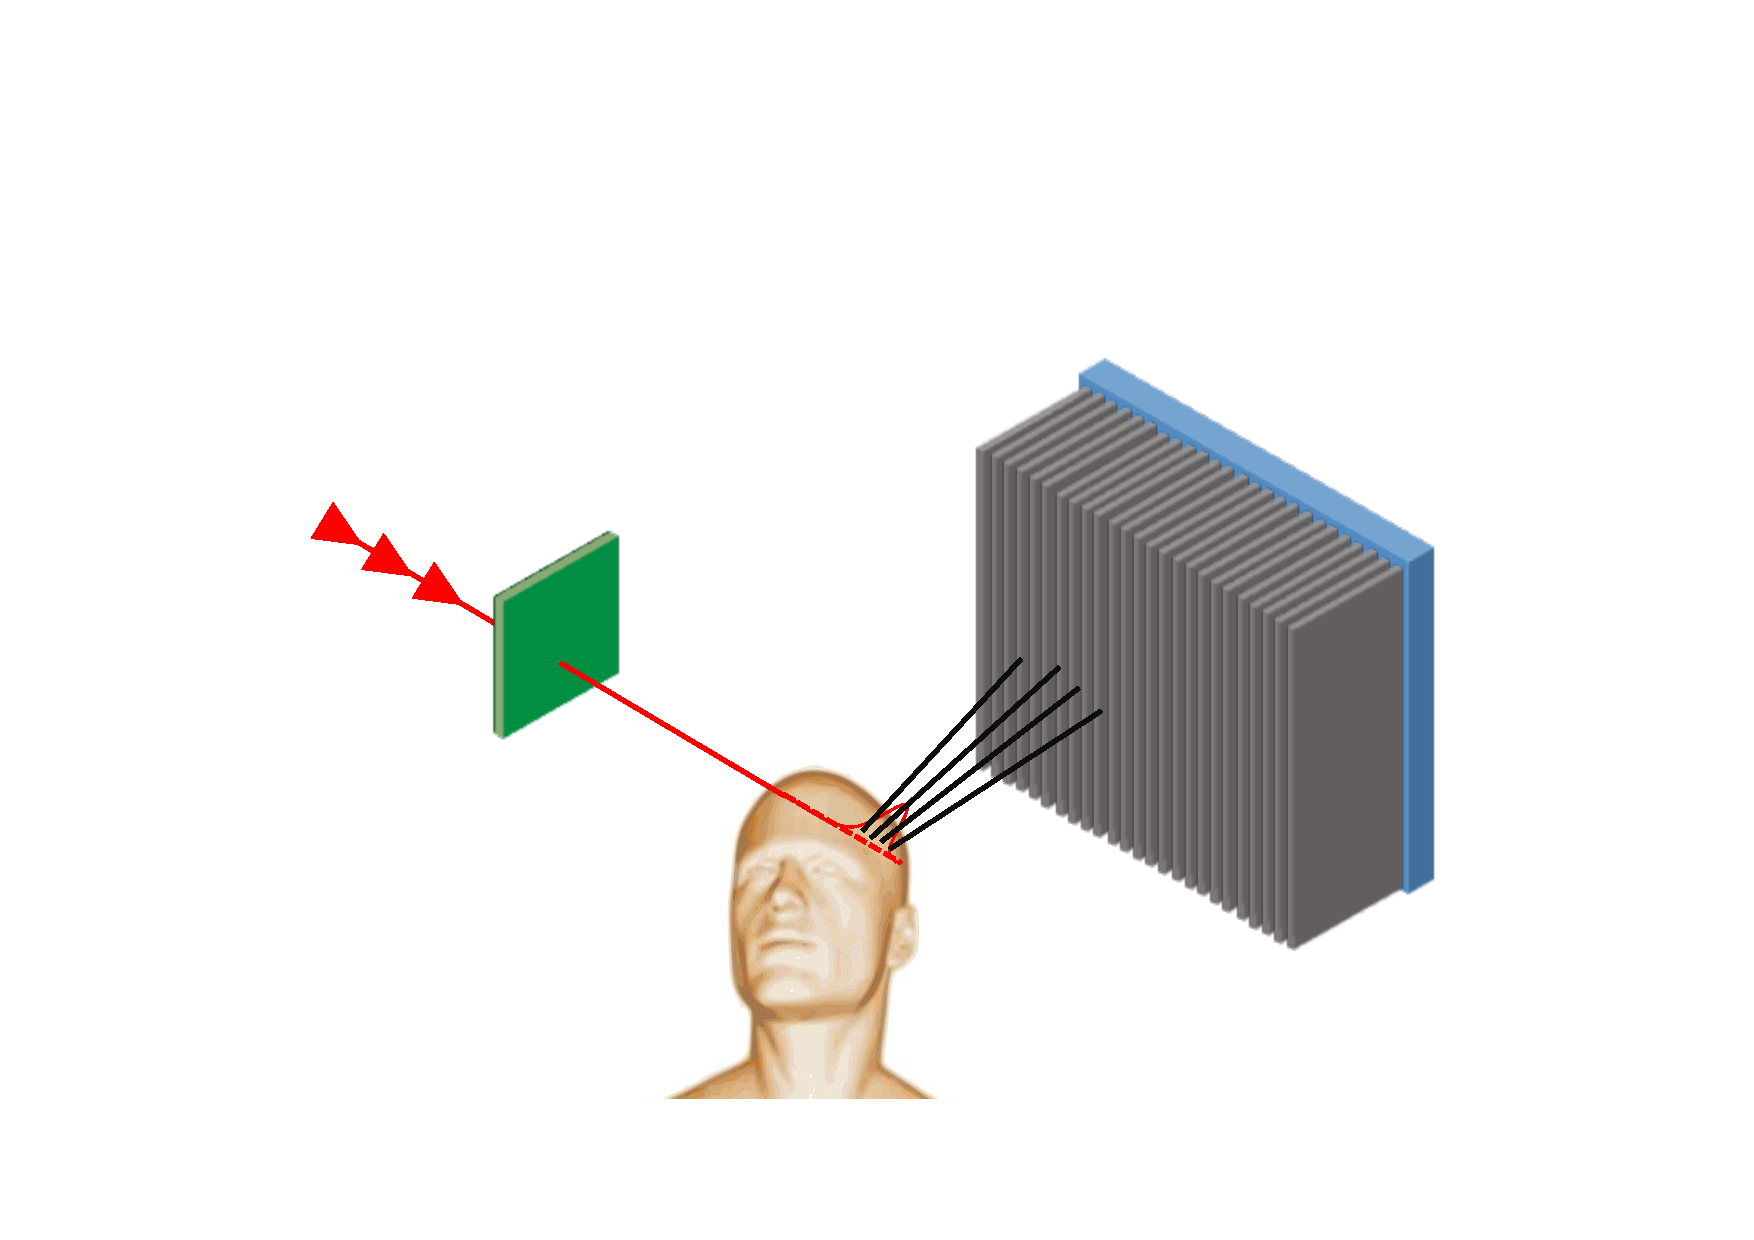
\includegraphics[width=1.2\textwidth]{03_GraphicFiles/chapter3_CLaRySproto/schemes/schema_Collimated_withHodo.pdf}
\caption{Scheme of the multi-collimated camera with the beam tagging hodoscope.}
\label{chap3::subfig::multiCollScheme}
\end{subfigure}
\begin{subfigure}[b]{.5\textwidth}
\centering
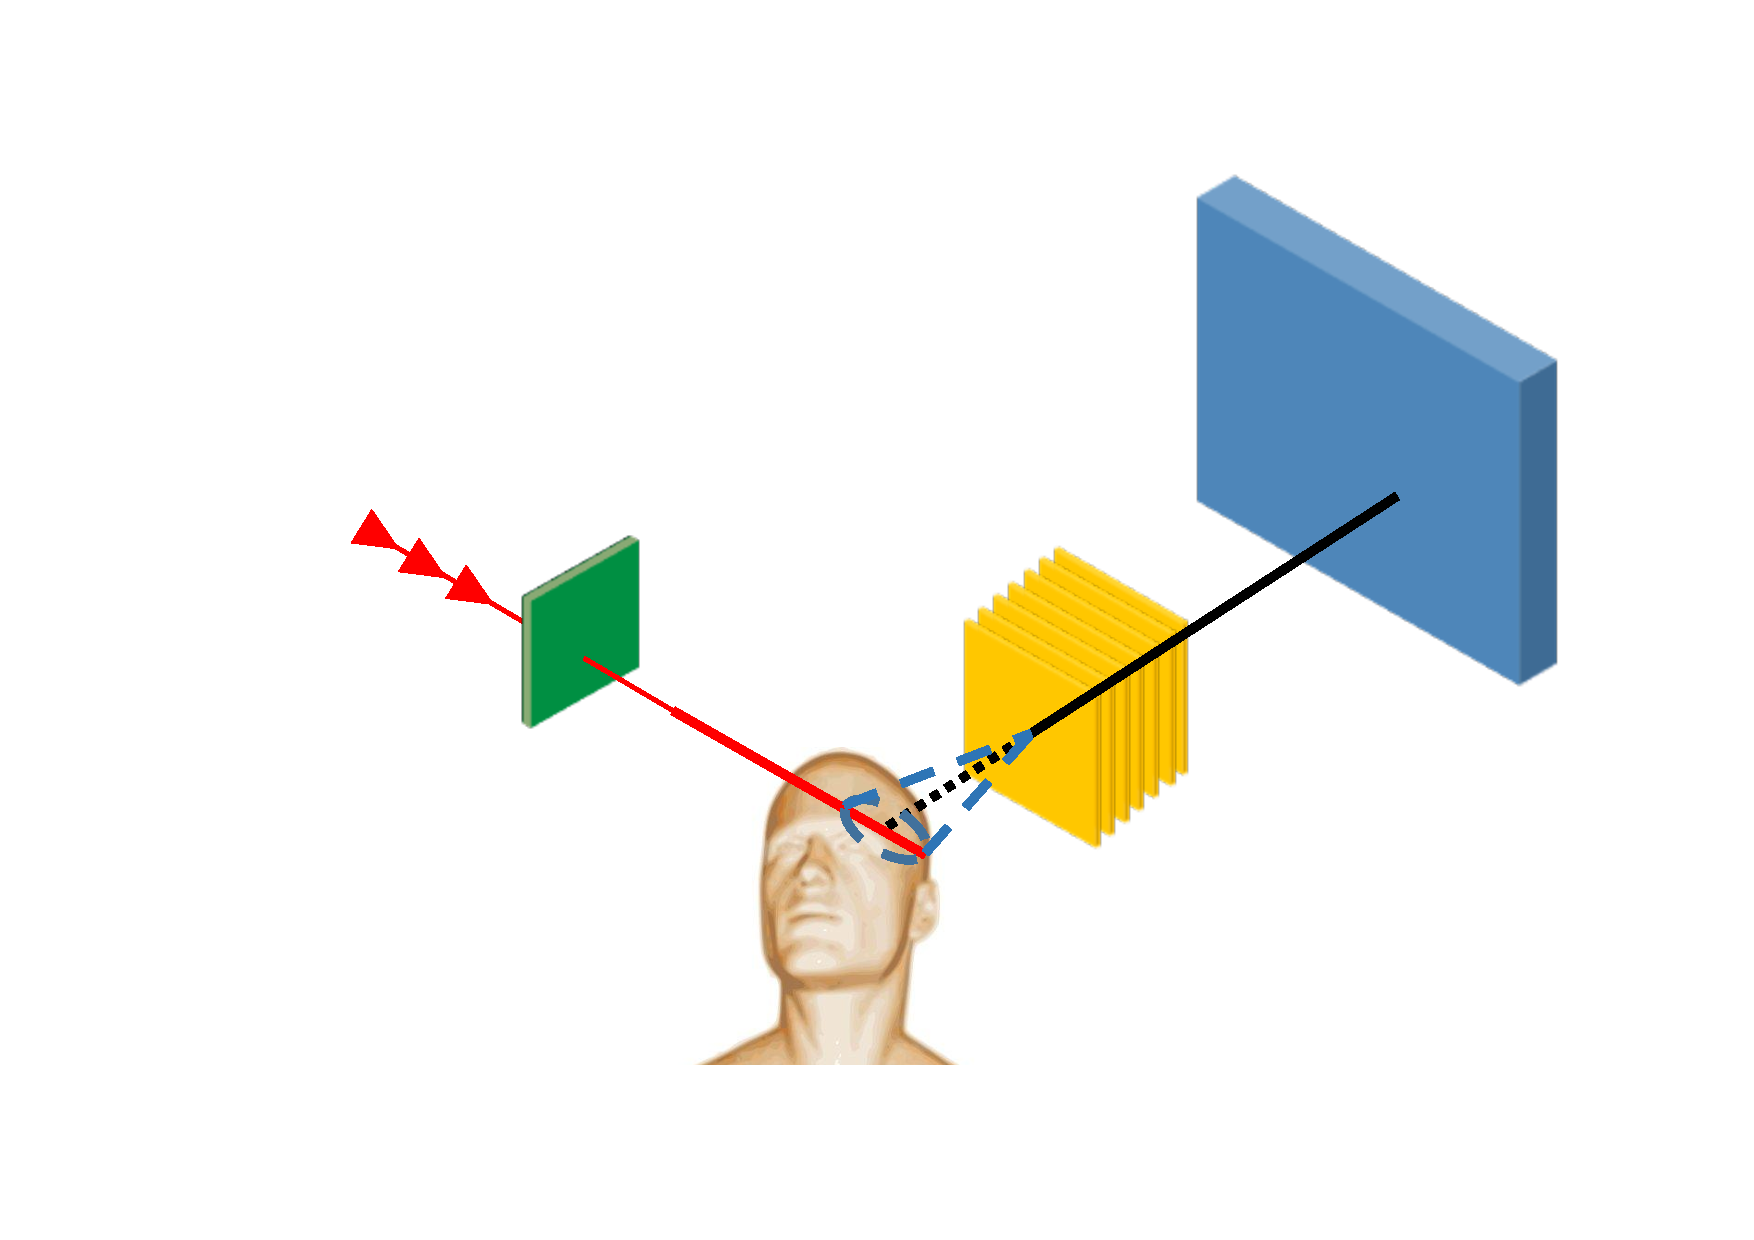
\includegraphics[width=1.2\textwidth]{03_GraphicFiles/chapter3_CLaRySproto/schemes/schema_Compton_withHodo.pdf}	
\caption{Scheme of the Compton camera with the beam tagging hodoscope.}
\label{chap3::subfig::ComptonScheme}
\end{subfigure}
\caption{Schematic view of the two CLaRyS gamma camera prototypes: the multi-collimated camera (a) and the Compton camera (b), both coupled to the beam tagging hodoscope. The ion beam is represented by the red line, and some beam bunches has been highlighted. The detection principle is also sketched for the two detectors: the tungsten collimator select the parallel incoming photons for the multi-slit collimated camera (a), while the Compton cone is reconstructed with the two interactions in scatterer and absorber in the Compton camera (b).}
\label{chap3::fig::camerasScheme}
\end{figure}
 

%%%%%%%%%%%%%%%%%%%%%%%%%%%%%%%%%%   SCATTERER  %%%%%%%%%%%%%%%%%%%%%%%%%%%%%%%%%%%%%%%%%%%%

\subsection{Scatterer}\label{chap3::subsec::scatterer} 
The scatterer stack is one of the components of the Compton camera prototype. Dedicated to the photon Compton scattering, its design has been studied to fulfill the camera requirements.\\ 
The Compton events reconstruction strongly relies on the measurement of the energy deposited by the photon in its Compton interaction, mandatory to properly calculate the Compton scattering angle, which is then the aperture of the resulting Compton cone. The camera accuracy is then strictly dependent on the scatterer energy resolution. At the same time, the camera efficiency is dominated by the balance between Compton interaction and photoelectric absorption probability in the scatterer detector.\\
Given the need of at least two interactions for a proper event reconstruction (a Compton scattering in the scatterer section and an ideally complete absorption in the absorber section, described in~\ref{chap3::subsec::absorber}), the material choice and the geometrical configuration play a fundamental role in the camera operation. The setup must be tuned in order to define the better trade-off between Compton and photoelectric interaction probability and to optimize, as mentioned, the detector energy resolution.\\
Given the fact that the Compton interaction probability linearly increases with the material atomic number (Z), while the photoelectric absorption depends on Z$^{n}$ with n varying between 4 and 5 according to the photon primary energy~\parencite{Knoll2000}, it is clear that a low Z material is preferred. Considering now the detector energy resolution, it must be noticed that the main parameter affecting the deposited energy detection is the so called \enquote{Doppler spread}. The Compton angle reconstruction formula in equation~\ref{chap1::eq::Compton} neglects the initial recoil electron state, which is considered free or unbound. The Compton energy transfer continuum results affected by the binding energy of the electron, with a relatively increasing effects for decreasing incident photon energy. This effect adds uncertainty on the reconstructed deposited energy, and so in the Compton angle calculation. Given its direct dependence on the recoil electron binding energy, the \enquote{Doppler spread} is reduced for low Z materials. Following the described theoretical considerations, silicon detectors are the most coherent choice. This choice has been verified in simulation, where a silicon scatterer has been compared to competitor materials; the result are included in the Monte Carlo study presented in chapter~\ref{chap::5}.\\
Dedicated Monte Carlo simulation studies have been performed in order to define the most suitable geometrical configuration for the Compton camera, including the scatterer stack~\parencite{Richard2012}. As a trade-off between detection efficiency and total cost, 10 layers were included in the original scatterer design. Concerning the layer size, about 10$\times$10~cm$^{2}$ of active area in the transverse plane have been identified as the most convenient choice, also considering the absorber size (see section~\ref{chap3::subsec::absorber}) and the distances between the detection sections required by the \gls{tof} measurements and imposed by the detector rate acceptance in clinical conditions (see appendix~\ref{chap::appA}). Moving to the layer thickness, its choice is governed by the definition of the camera operation. The \gls{clarys} Compton camera does not aim to track the Compton recoil electron, which must be then absorbed inside the same scatterer layer where the Compton interaction took place. This requirement is necessary to well reconstruct the Compton interaction angle, which needs the whole transferred energy as parameter; in addition to this, a recoil electron escaping the involved detection layer can interact in a different layer causing false coincidences which affect the camera efficiency and imaging accuracy. In order to minimize the recoil electron escape probability, relatively thick detectors are needed.\\
The technological choice of the collaboration was oriented to silicon \glspl{dssd}, provided by the Norwegian company SINTEF. A schematic view of the detector principle is given in \figurename~\ref{chap3::fig::dssdTHEO}. The silicon crystal is doped with negative (n) and positive (p) charge carriers on the two opposite sides, creating diodes which are then reverse biased. A polarization voltage is applied to the two opposite sides of the crystal, and a depletion region with no free charges is created. A ionizing particle interacting in the depletion region generates electron-hole pairs in number proportional to the deposited energy. The generated charges drift towards anode (electrons) and cathode (holes) and are converted into electrical signals. The read-out is ensured by the implanted strips, which transfer the charges outside the detection region.\\     

\begin{figure}
\begin{subfigure}[t]{.5\textwidth}
\centering
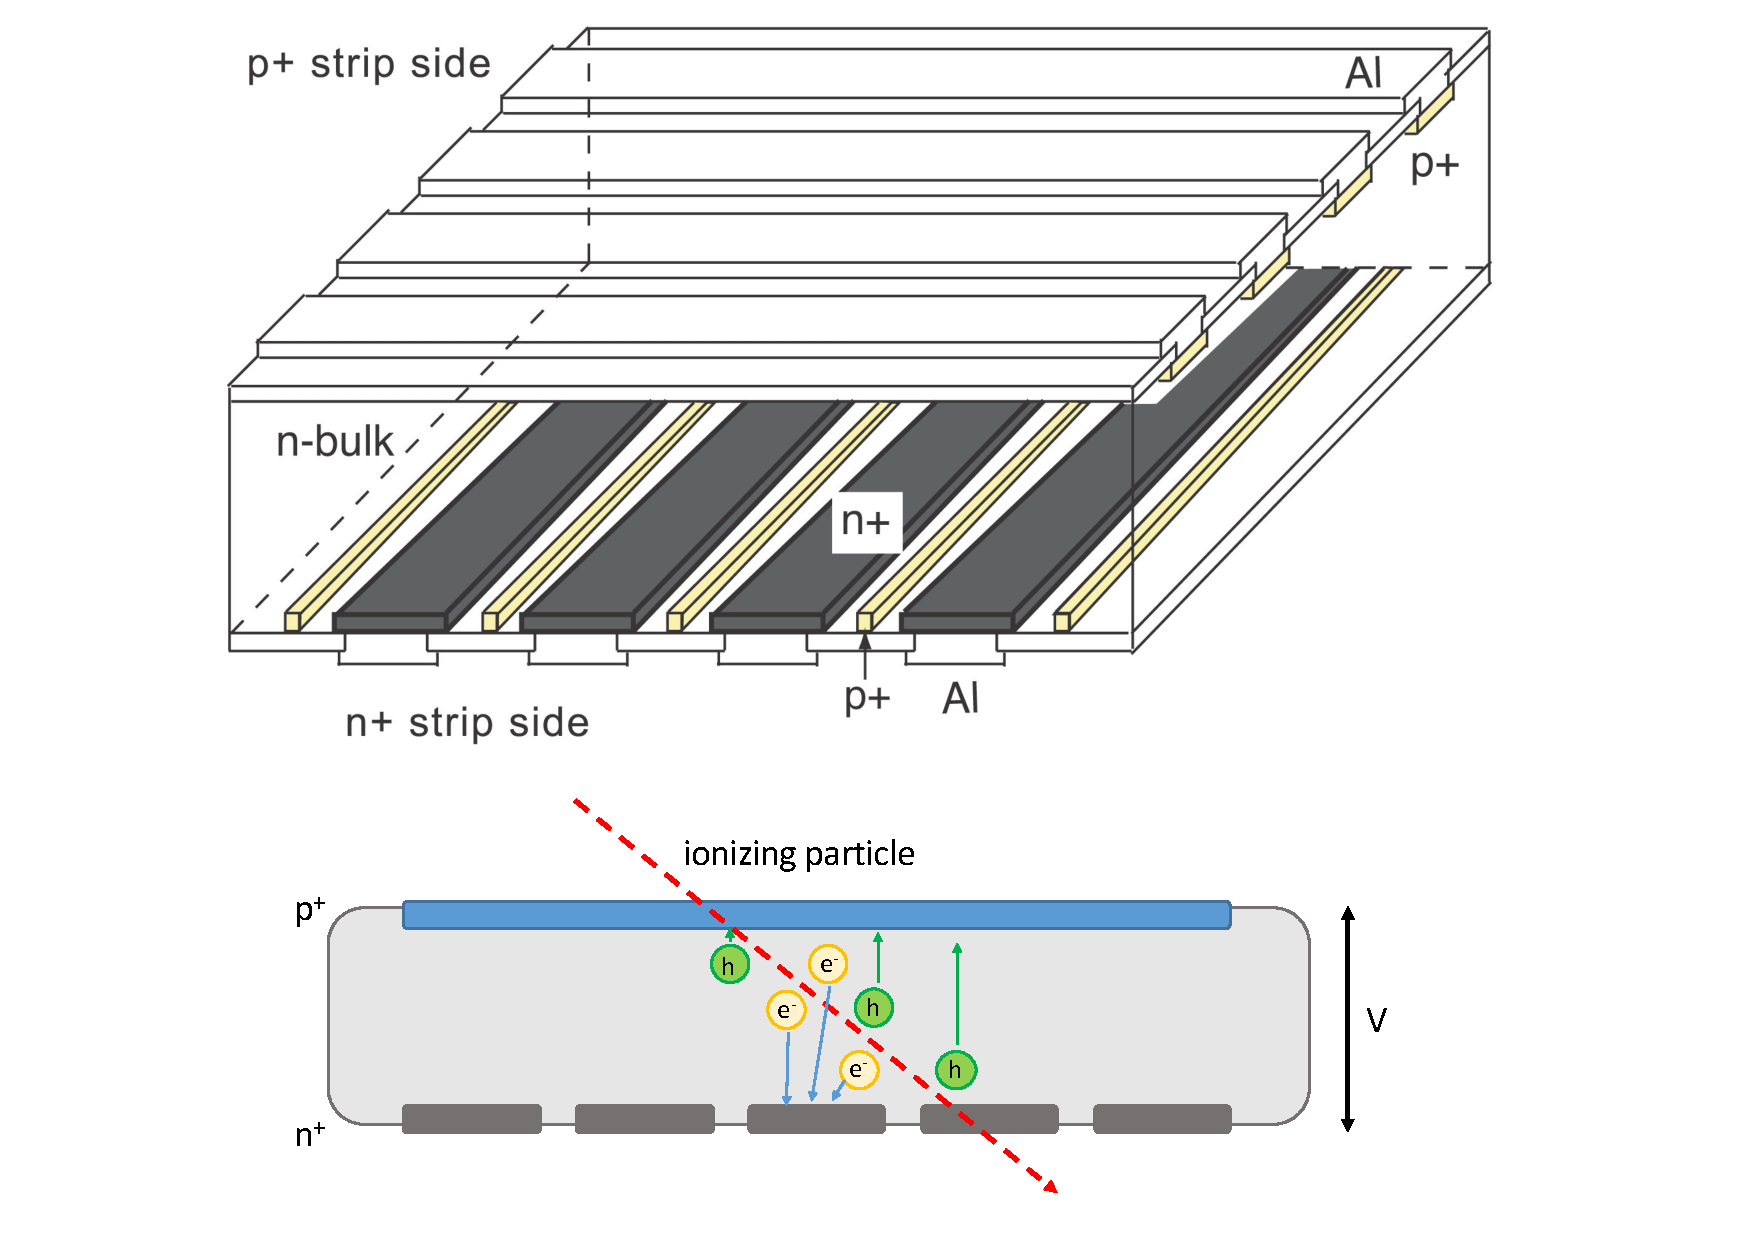
\includegraphics[width=1\textwidth]{03_GraphicFiles/chapter3_CLaRySproto/Scatterer/DSSD_theory_1.pdf}
\caption{Schematic view of a standard \gls{dssd} (from~\cite{Takeda2008}) and sketch of the signal generation.}
\label{chap3::fig::dssdTHEO}
\end{subfigure}
\begin{subfigure}[t]{.5\textwidth}
\centering
\includegraphics[width=1\textwidth, height=16em]{03_GraphicFiles/chapter3_CLaRySproto/Scatterer/ScattererThermalBox.JPG}
\caption{Scatterer silicon layer with its \gls{fe} card in the thermal regulated box (described in section~\ref{chap3::subsubsec::ScattThermBox}).}
\label{chap3::fig::ScattPicture}
\end{subfigure}
\caption{Overview of the scatterer layers, with its working principle (a) and a picture of the detector connected to the \gls{fe} card in the thermal regulated box (b).}
\label{chap3::fig::scatterer}
\end{figure} 

Each layer has an active volume of 96$\times$96$\times$2~mm$^{3}$, segmented with 64 strips per detection plane. The strip pitch is 1.41~mm, for a strip width of 1.31~mm. The applied polarization voltage is nominally -750~V, and it is uniformly shared on the whole surface to obtain a homogeneous depletion region. A guard ring, composed of 23 strips surrounding the read-out ones on the p side, ensures the desired voltage gradient. The more peripheral strip of the guard ring is connected to the high voltage, while the n side has a single strip for the guard ring, connected to the ground. The p and n read-out strips are then connected to the \gls{fe} electronics via bonding cables.\\
The \gls{fe} electronics card has been developed by the \gls{ipnl} electronics group and is described in details in section~\ref{chap3::subsubsec::ScattFEcard}. The silicon detector is directly plugged on the card, and the mechanical support for the scatterer stack has been studied according to the card size, as shown in \figurename~\ref{chap3::fig::ScattPicture}.\\   
Among the 10 received \glspl{dssd}, only 7 fulfilled the requirements imposed by the Compton camera application, mainly in terms of noise level (leakage current); 3 layer have been rejected, so that the final prototype scatterer is composed of 7 silicon planes.\\
The 7 selected layers have been characterized with a temporary acquisition system in terms of leakage current at different temperatures. The results of these measurements can be found in~\cite{Ley2015}. The measurements allowed to verify the producer specifications in terms of polarization voltage to be applied for a complete detector depletion, as well as to identify the noisy strips and create a complete characterization database. In addition to this, they highlighted the need to cool the detectors down with respect to the room temperature (25\textdegree{}C) in order to reduce the leakage current to acceptable levels, and so reducing the total noise level, affecting the detector performance. In order to accomplish the cooling task and respect, at the same time, the clinical restrictions, a thermal regulated box based on cold air pump has been designed and produced. It operates as the scatterer stack mechanical support, and it is described in section~\ref{chap3::subsubsec::ScattThermBox}.\\
      
 

\subsubsection{Scatterer Front-End card}\label{chap3::subsubsec::ScattFEcard}
As mentioned in the previous paragraph, the main requirement for the scatterer detector modules is a very good energy resolution. The desired working performance can be quantified as follows:
\begin{itemize}
\item 1~keV \gls{fwhm} energy resolution;
\item 1.41~mm spatial resolution (corresponding to the strip pitch);
\item 15~ns \gls{fwhm} time resolution.
\end{itemize} 

The scatterer \gls{fe} card has been developed by the \gls{ipnl} electronics group in order to achieve this performance. It is composed of two well separated sections, analog and digital, which must be kept separated in the card layout in order to minimize the contribution of the digital noise on the treatment of the analog signals. Moreover, in order to reduce the electronic noise, the analog section must be placed as close as possible to the detector, to minimize the signal path length.\\
At first, a dedicated \gls{asic} has been designed and developed to treat the signals directly coming from the \gls{dssd}~\parencite{Dahoumane2014}. Each \gls{asic} 
processes 8 detectors channels, so that 8 \gls{asic} per plane are required for the read-out of a complete silicon layer. This section represents the core of the analog stage. The \gls{asic} has been designed and tested to achieve the desired performance in terms of \gls{enc}, which must be lower than 118 electrons \gls{rms} in order to obtain the 1~keV \gls{fwhm} energy resolution, signal dynamics and accepted detection rate. The analog raw signal first passes through a \gls{csa}, which returns an analog amplified signal. This pulse can be further amplified with a \gls{shs} based on a \gls{cr-rc} filter, which filters and shapes the signal in about 1~\charmus, or via a fast amplifier (with 15~ns shaping time). The first mode is used for a refined charge (deposited energy) measurement and can be employed for detector tests and characterization, while the second is the standard working one which allows for fast energy and time measurements. The amplified signal finally passes through a discriminator, which gives a digital output. Analog (from \gls{csa} or \gls{shs}) and digital signals are then sent to the digital stage of the card for the measurement of time, position and energy. To be noticed \\
The digital stage is mainly composed of one \gls{adc} module per \gls{asic} and two \glspl{fpga}. The analog signal from the \gls{asic} is processed by the \gls{adc}, which is a 12-bit module with 8 channels, with a sampling rate of 100~\gls{mpsp}. Each \gls{adc} returns 16 \gls{lvds} pairs (2 per channel), which are sent to the \glspl{fpga} together with two clock signals (two \gls{lvds} pairs) and the 8 digital outputs of the \gls{asic}. So, 44 input channels of the \gls{fpga} are used for the acquisition of 8 read-out channels (one \gls{asic}). Two \glspl{fpga} Altera Cyclone III~\parencite{Altera2012} are installed on the card to handle the signals coming from the whole detector (128 channels, 64 per detection plane): both of them are equipped with a \gls{tdc} for the time measurement.\\
A third \gls{fpga} (Altera StratixII GX~\parencite{Altera2009}) is finally installed on the card to handle the processed data collection and the communication with the acquisition system, described in section~\ref{chap3::subsec::cameraElectronicsDAQ}, via a 3~Gbit/s link.\\
The \gls{asic} has been developed in three versions, and the cards have been optimized during the development process and produced in its final version (shown in \figurename~\ref{chap3::fig::scattDAQcard}) in the spring 2017. The 7 cards are now available and the development of the \gls{fpga} firmware is ongoing.\\
More details about the card layout, components and operating principle, as well as a description of the tests performed during the development can be found in~\cite{Chen2017} and~\cite{Dahoumane2012}.    

\subsubsection{Scatterer thermal regulated box}\label{chap3::subsubsec::ScattThermBox}

The results of the leakage current tests performed on the silicon detectors showed the need of cooling the detector down to achieve the required performance in terms of noise, which affects the spatial, time and energy resolutions. The leakage current has been studied in temperature cycles in the range -40 - +40~\textdegree{}C, and an overall consistent behavior has been observed both on N and P strips of the detector. The leakage current slightly increases in the range -40 - 0~\textdegree{}C, with values in the range 0 - 8~nA for the analyzed strips, and then drastically increases beyond 0~\textdegree{}C, with peaks of more then 80~nA at +40~\textdegree{}C. The complete description of the performed measurements and the detailed results can be found in~\cite{Ley2015}.\\
A cooling system is needed for the silicon detectors operations: it must be able to keep the temperature constant and below, at least, 0~\textdegree{}C, preferably around -20~\textdegree{}C where the leakage current is more stable in case of small temperature variations. The clinical environment limitations must be considered to design such a cooling system (portability, gas, noise level), as well as the material budget and the mechanical integration with the other camera components.\\
The implemented solution consists in the thermal regulated box shown in \figurename~\ref{chap3::fig::ScattPicture}, together with one of the silicon layers. The size of the box is 490$\times$490$\times$300~mm$^3$, and the structure is composed of 2~mm of aluminum and three insulation layers of 10~mm of silica aerogel Spaceloft\textsuperscript{\textregistered}~\parencite{Spaceloft2011}, for an equivalent thickness of 2~mm of silicon (0.7\% of interaction probability for 1~MeV photons). The cooling is performed via an electric air pump, which is able to keep the temperature inside the box at -20~\textdegree{}C with a 400~W haet evacuation power. The heat power produced by the 7 silicon \gls{fe} cards in operation must be verified, but the estimate confirms the effectiveness of the thermal box nominal performance. Once card and detector will be fully operational, a test will be performed to check the temperature stability inside the box.\\
The 	\gls{fe} cards and the silicon layers are fixed inside the box via a mechanical support designed and produced by the \gls{ipnl} mechanics group. The support, which ensures a millimeter position accuracy, is fixed on metal rails which allow to easily handle each detector layer. A scheme of the thermal box and the internal support is shown in \figurename~\ref{chap3::fig::thermalBox}.
    
\begin{figure}
\begin{subfigure}[t]{.5\textwidth}
\centering
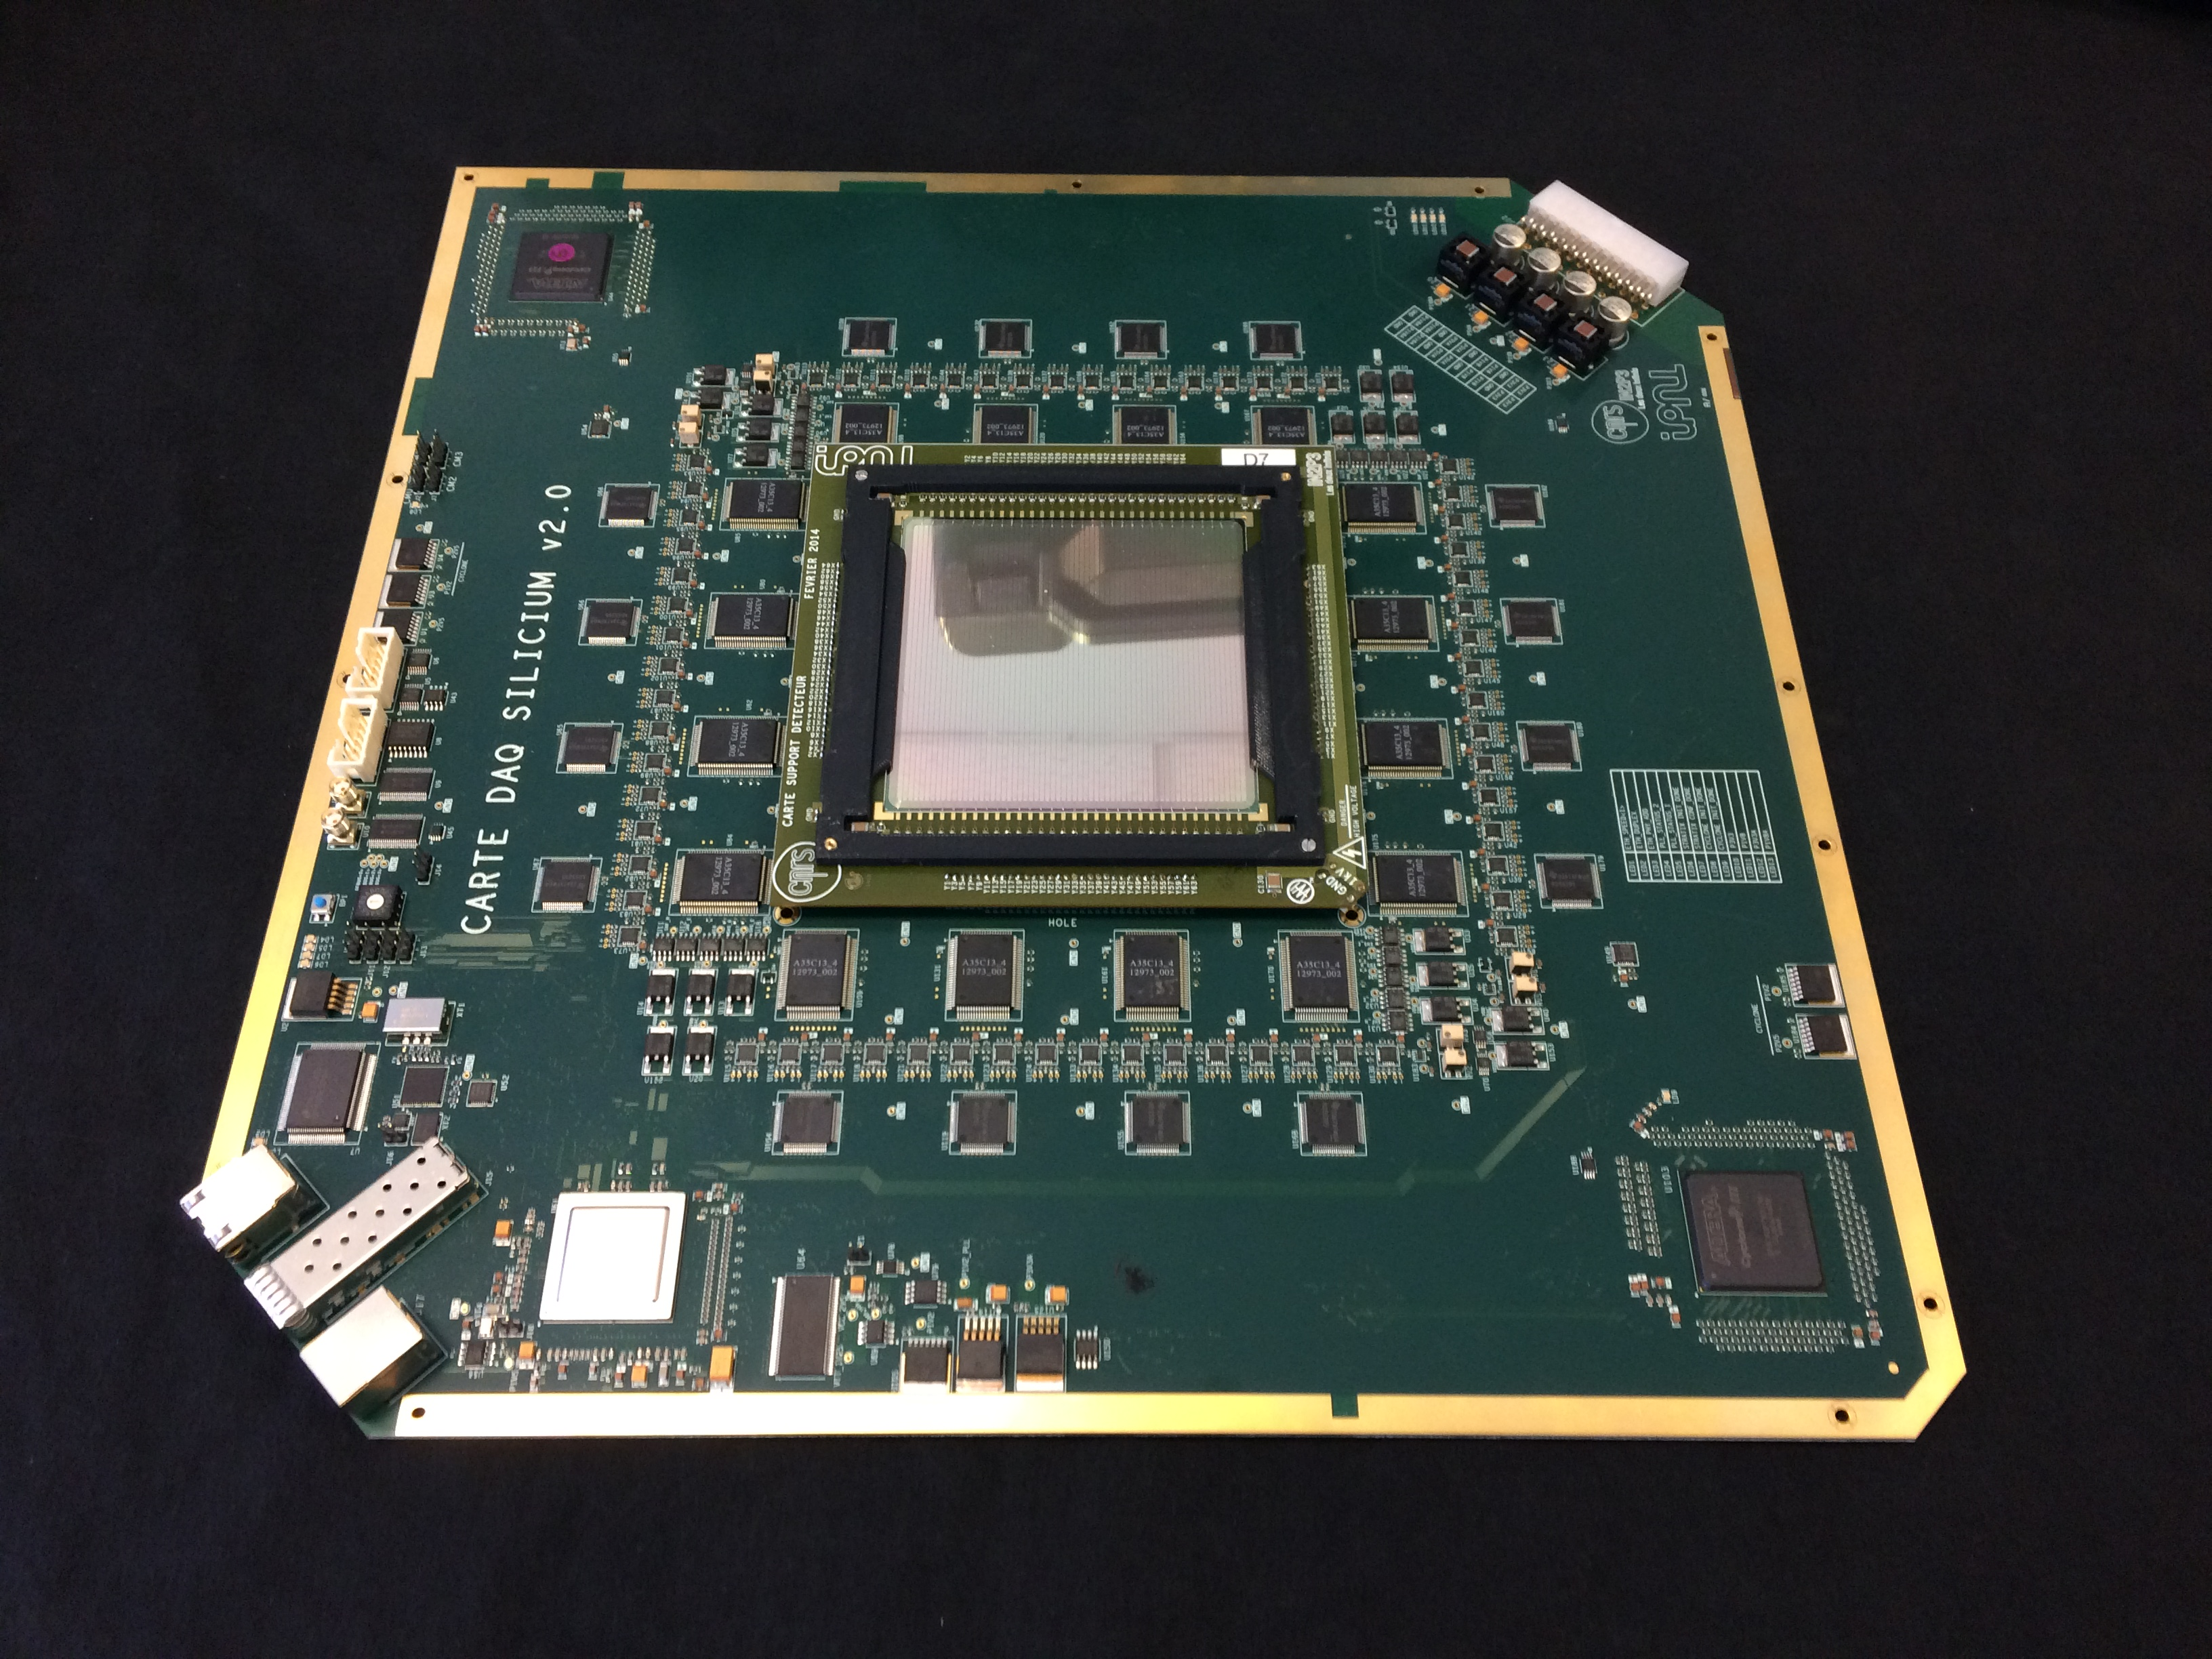
\includegraphics[width=1\textwidth, height = 5.7cm]{03_GraphicFiles/chapter3_CLaRySproto/Scatterer/DAQ_card.JPG}
\caption{Final version of the scatterer \gls{fe} card with the silicon detector layer.}
\label{chap3::fig::scattDAQcard}
\end{subfigure}
\begin{subfigure}[t]{.5\textwidth}
\centering
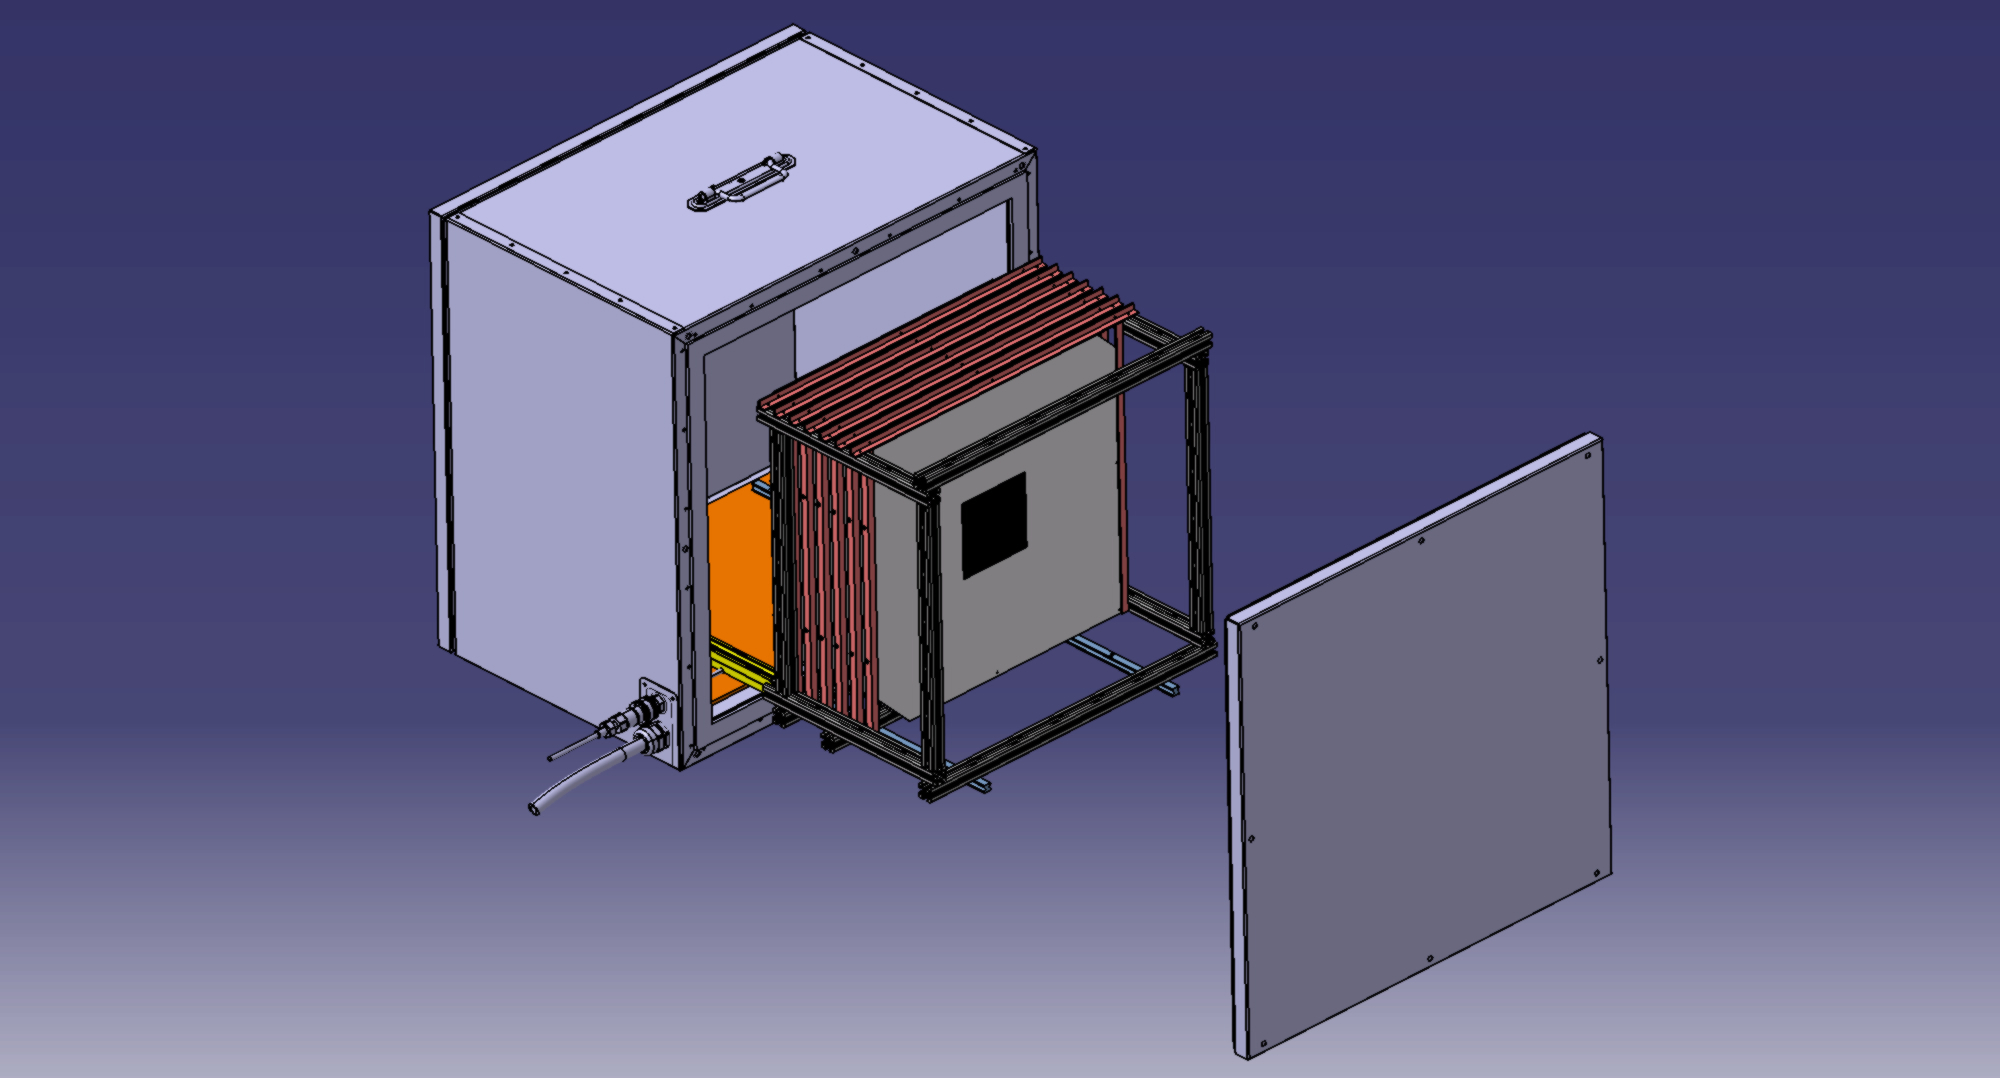
\includegraphics[width=1\textwidth, trim={5cm 0 5cm 0}, clip = true, height = 5.7cm]{03_GraphicFiles/chapter3_CLaRySproto/Scatterer/Rack_cartes_Si_2.jpg}
\caption{Scheme of the scatterer stack thermal box and internal mechanical support.}
\label{chap3::fig::thermalBox}
\end{subfigure}
\caption{Scatterer silicon layers equipment: final version of the \gls{fe} card (a) and scheme of the detector integration in the thermal regulated box (b).}
\label{chap3::fig::scattererCardMech}
\end{figure} 

%%%%%%%%%%%%%%%%%%%%%%%%%%%%%%%%%%   COLLIMATOR  %%%%%%%%%%%%%%%%%%%%%%%%%%%%%%%%%%%%%%%%%%%%

\subsection{Collimator}\label{chap3::subsec::collimator}
 
The multi-collimated camera is equipped with a multi-slit collimator, with tungsten slabs. Its design has been extensively studied in Monte Carlo simulations~\parencite{Pinto2014}, and it can be easily adapted to different geometrical configurations of the absorber detector and to various monitoring requirements. In particular, the distance between neighboring slabs can be modified, as well as the number of total slabs, in order to find the best trade-off between detection efficiency and spatial resolution; this depends on the distance patient-collimator, on the required extension of the field of view and on the desired monitoring time. Two identical collimators of 30$\times$14$\times$17~cm$^{3}$ have been produced, in order to be able to set several absorber configurations in the transverse direction (extended version along the beam axis or in the perpendicular direction). In \figurename~\ref{chap3::fig::collimatorPicture} a picture of the tungsten collimator is presented, while in \figurename~\ref{chap3::fig::collimatorScheme} we show a schematic view of a possible multi-collimated camera configuration.\\

\begin{figure}
\begin{subfigure}[t]{.5\textwidth}
\centering
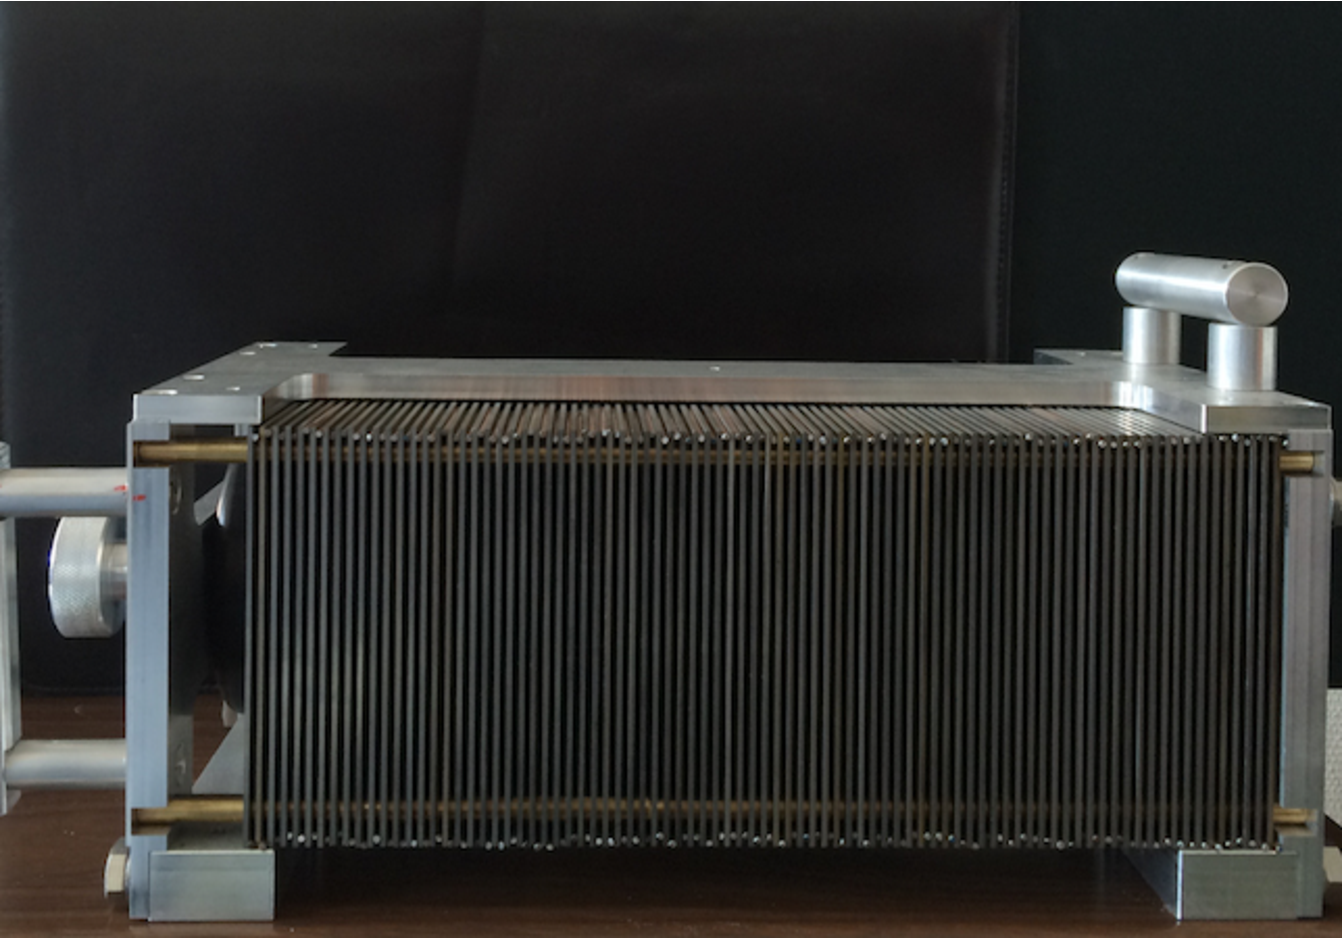
\includegraphics[width=\linewidth, trim={0 0 0 0.5cm},clip = true, height = 5cm]{03_GraphicFiles/chapter3_CLaRySproto/Collimator/Collimator.pdf}
\caption{Multi-slit tungsten collimator.}
\label{chap3::fig::collimatorPicture}
\end{subfigure}
\begin{subfigure}[t]{.5\textwidth}
\centering
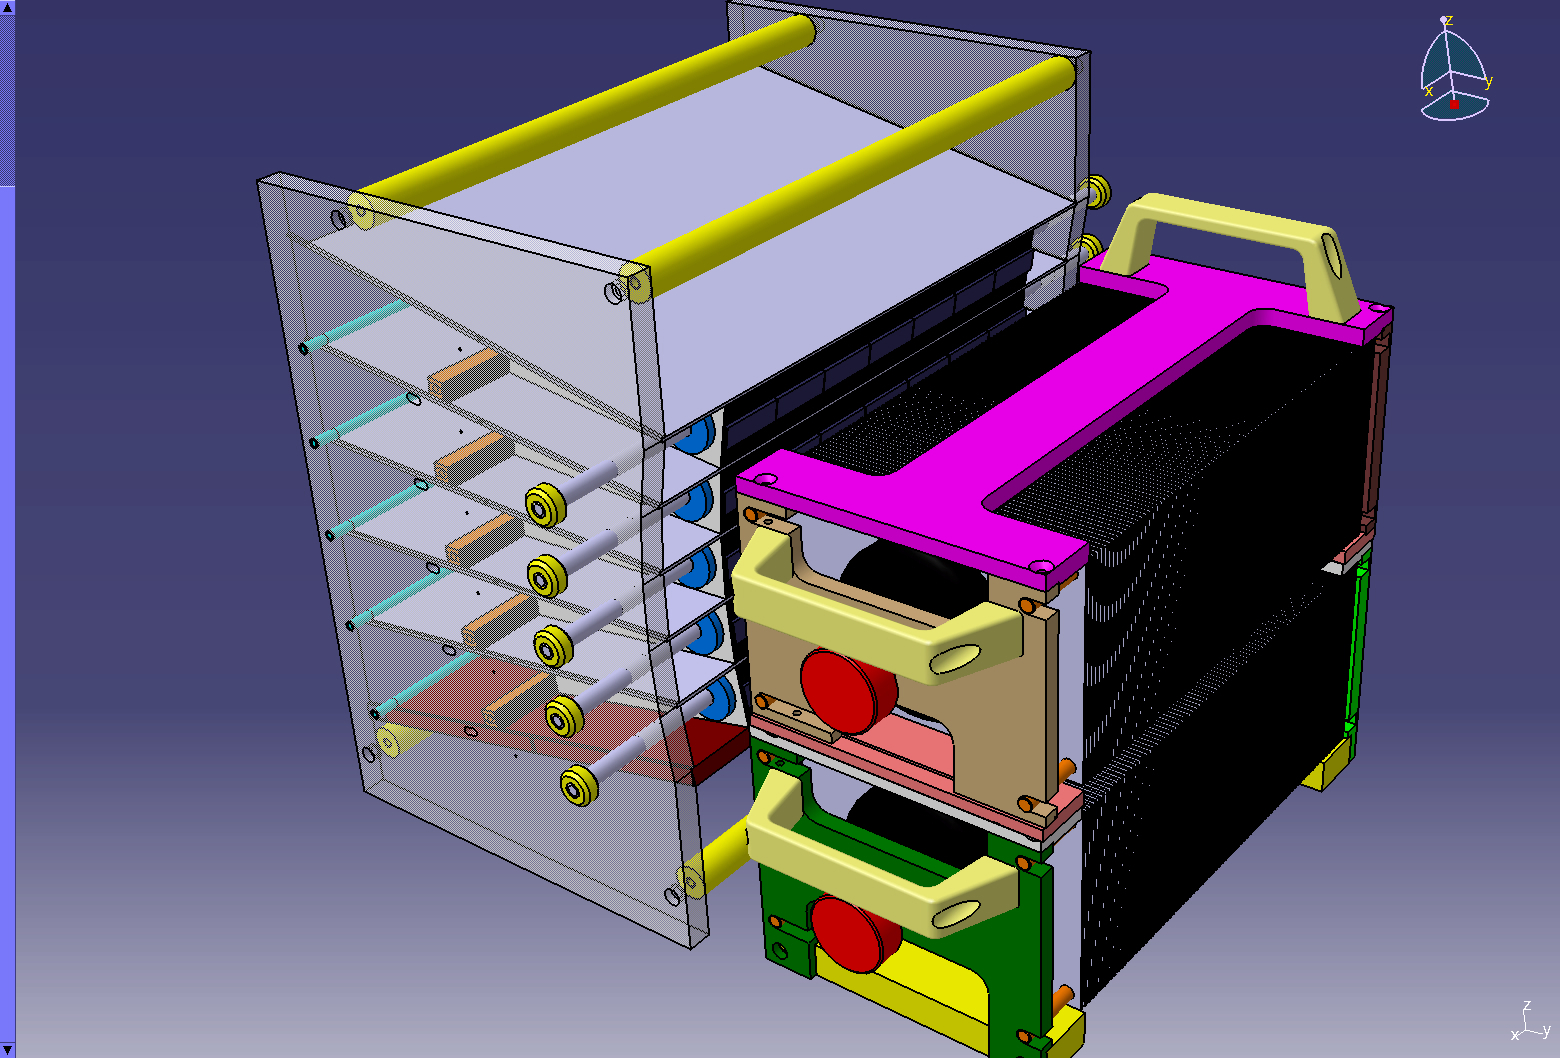
\includegraphics[width=\linewidth, trim={3cm 0 0 0},clip = true, height = 5cm]{03_GraphicFiles/chapter3_CLaRySproto/schemes/AbsoberCollimator.jpg}
\caption{Scheme of the multi-slit collimated camera configuration.}
\label{chap3::fig::collimatorScheme}
\end{subfigure}
\caption{Tungsten collimator and its setup in the multi-slit collimated camera. The two tungsten multi-slit collimators are placed in front of a 6$\times$5 \gls{bgo} block absorber setup in its mechanical support (see section~\ref{chap3::subsec::absorber}).}
\label{chap3::fig::collimatorFig}
\end{figure} 


%%%%%%%%%%%%%%%%%%%%%%%%%%%%%%%%%%   ABSORBER  %%%%%%%%%%%%%%%%%%%%%%%%%%%%%%%%%%%%%%%%%%%%

\subsection{Absorber}\label{chap3::subsec::absorber}

The Compton and multi-collimated camera absorber was initially conceived as a very large surface plane composed of 96 \gls{bgo} blocks recovered from a dismantled \gls{pet} system HR+ by SIEMENS, documented in~\parencite{Adam1997, Brix1997}.\\ 
%%%From BGO paper %%%%%%%%
\gls{bgo} is one of the most used scintillators for gamma detection applications, thanks to a good energy resolution and a optimal gamma detection efficiency. Moreover, the absence of internal radioactivity which characterizes other scintillator materials employed in the same field (i.e.~\gls{lyso}, \gls{lso}), makes it suitable for low noise detectors, required by a Compton camera to reduce the amount of random coincidences, one of the main sources of background for the application in ion beam therapy monitoring~\parencite{Ortega2015}. As highlighted in~\parencite{HuesoGonzalez2015}, \gls{lyso} and \gls{lso} show overall better performances with respect to \gls{bgo} for what concerns energy, time and spatial resolution, due to an about 4 times higher light yield, but the gap is reduced for the detection of gamma rays in the prompt-gamma energy range (especially beyond 1~MeV). The limited cost of \gls{bgo} with respect to \gls{lso} and the comparable performances in the prompt-gamma energy range make it an optimal solution for prompt-gamma camera prototypes.\\
Each \gls{bgo} block has a surface of 3.5$\times$3.8~cm$^2$, with a thickness of 3.0~cm. The mono-block \gls{bgo} crystal is streaked in a 8$\times$8 pseudo-pixel matrix; a reflecting material is inserted between the pseudo-pixels to improve the light collection and optimize the spatial information accuracy via pixel separation. The read-out is achieved via four \gls{pm} tubes per block, composing a quartet, coupled to the block back surface. Thanks to the internal streaked structure of the block, the scintillation light is shared on the four \glspl{pm} depending on the pseudo-pixel where the interaction takes place (in case of multiple interactions more than 1 pseudo-pixel can be involved). The streaks have a different thickness according to their position in the block: they fully cover the block thickness on the block borders and they progressively shorten towards the block center, with a mono-block structure in the central block section on the entrance face. The reconstruction of the position of interaction is done via Anger logic, i.e.~with a center of gravity calculation.\\
The whole set of recovered blocks was supposed to undergo a \enquote{reconditioning} process, including the \gls{pm} removal, the crystal back surface polishing with diamond-based abrasive tool, the single \glspl{pm} gain characterization and grouping in quartets with similar gains, the final re-coupling of the \glspl{pm} and block shielding.\\ A set of \enquote{reconditioned} blocks have been tested with the method described in section~\ref{chap3::sec::charMeasurements} and their performance have been compared to a set of original blocks. An overall degradation of the detection performance has been verified on all the tested \enquote{reconditioned} blocks, which showed lower amplitude output signals probably link to a reduction of the collected scintillation light. Various correction methods have been tested, with unsatisfactory results. According to the outcome of these tests, summarized in~\cite{Sandjong2017}, the collaboration finally opted to adapt the camera design for the use of original, \enquote{non-reconditioned} \gls{bgo} blocks.\\    
Thirty original blocks are now available to compose the absorber detector. In addition to the already presented features, it must be noticed that the lateral surfaces of the original blocks, as well as the half of the \gls{pm} length, are covered by a reflecting material which ensures the complete collection of the scintillation light. This is probably a component which was not well reproduced during the reconditioning process. The whole structure is then protected by a 1~mm thick aluminum foil, which also isolates from external light contamination.\\
\figurename~\ref{chap3::fig::block_noPM} shows one \gls{bgo} block before the coupling to the \gls{pm} quartet: the streaked structure is clearly visible, as well as the white reflecting material separating the pseudo-pixels and the one surrounding the block lateral sides. As mentioned, the same material also covers part of the photo-multiplier tubes, as shown in picture~\ref{chap3::fig::originalBlock_noAl}, where the four \glspl{pm} are glued to the block back surface. The described aluminum cover is visible in \figurename~\ref{chap3::fig::originalBlock_withAl}, while in \figurename~\ref{chap3::fig::BGOblockScheme} a scheme of a block together with the related \gls{pm} quartet is given. The spatial reconstruction logic is also reported in the same figure. To be noticed that the streaked structure of the pseudo-pixels depends on their position in the block: the reflecting streak covers about three fourth of the block thickness for the for the lateral pseudo-pixels, while it is limited to half of the block thickness for the central ones.\\ 

\begin{figure}
\begin{subfigure}[t]{.5\textwidth}
\centering
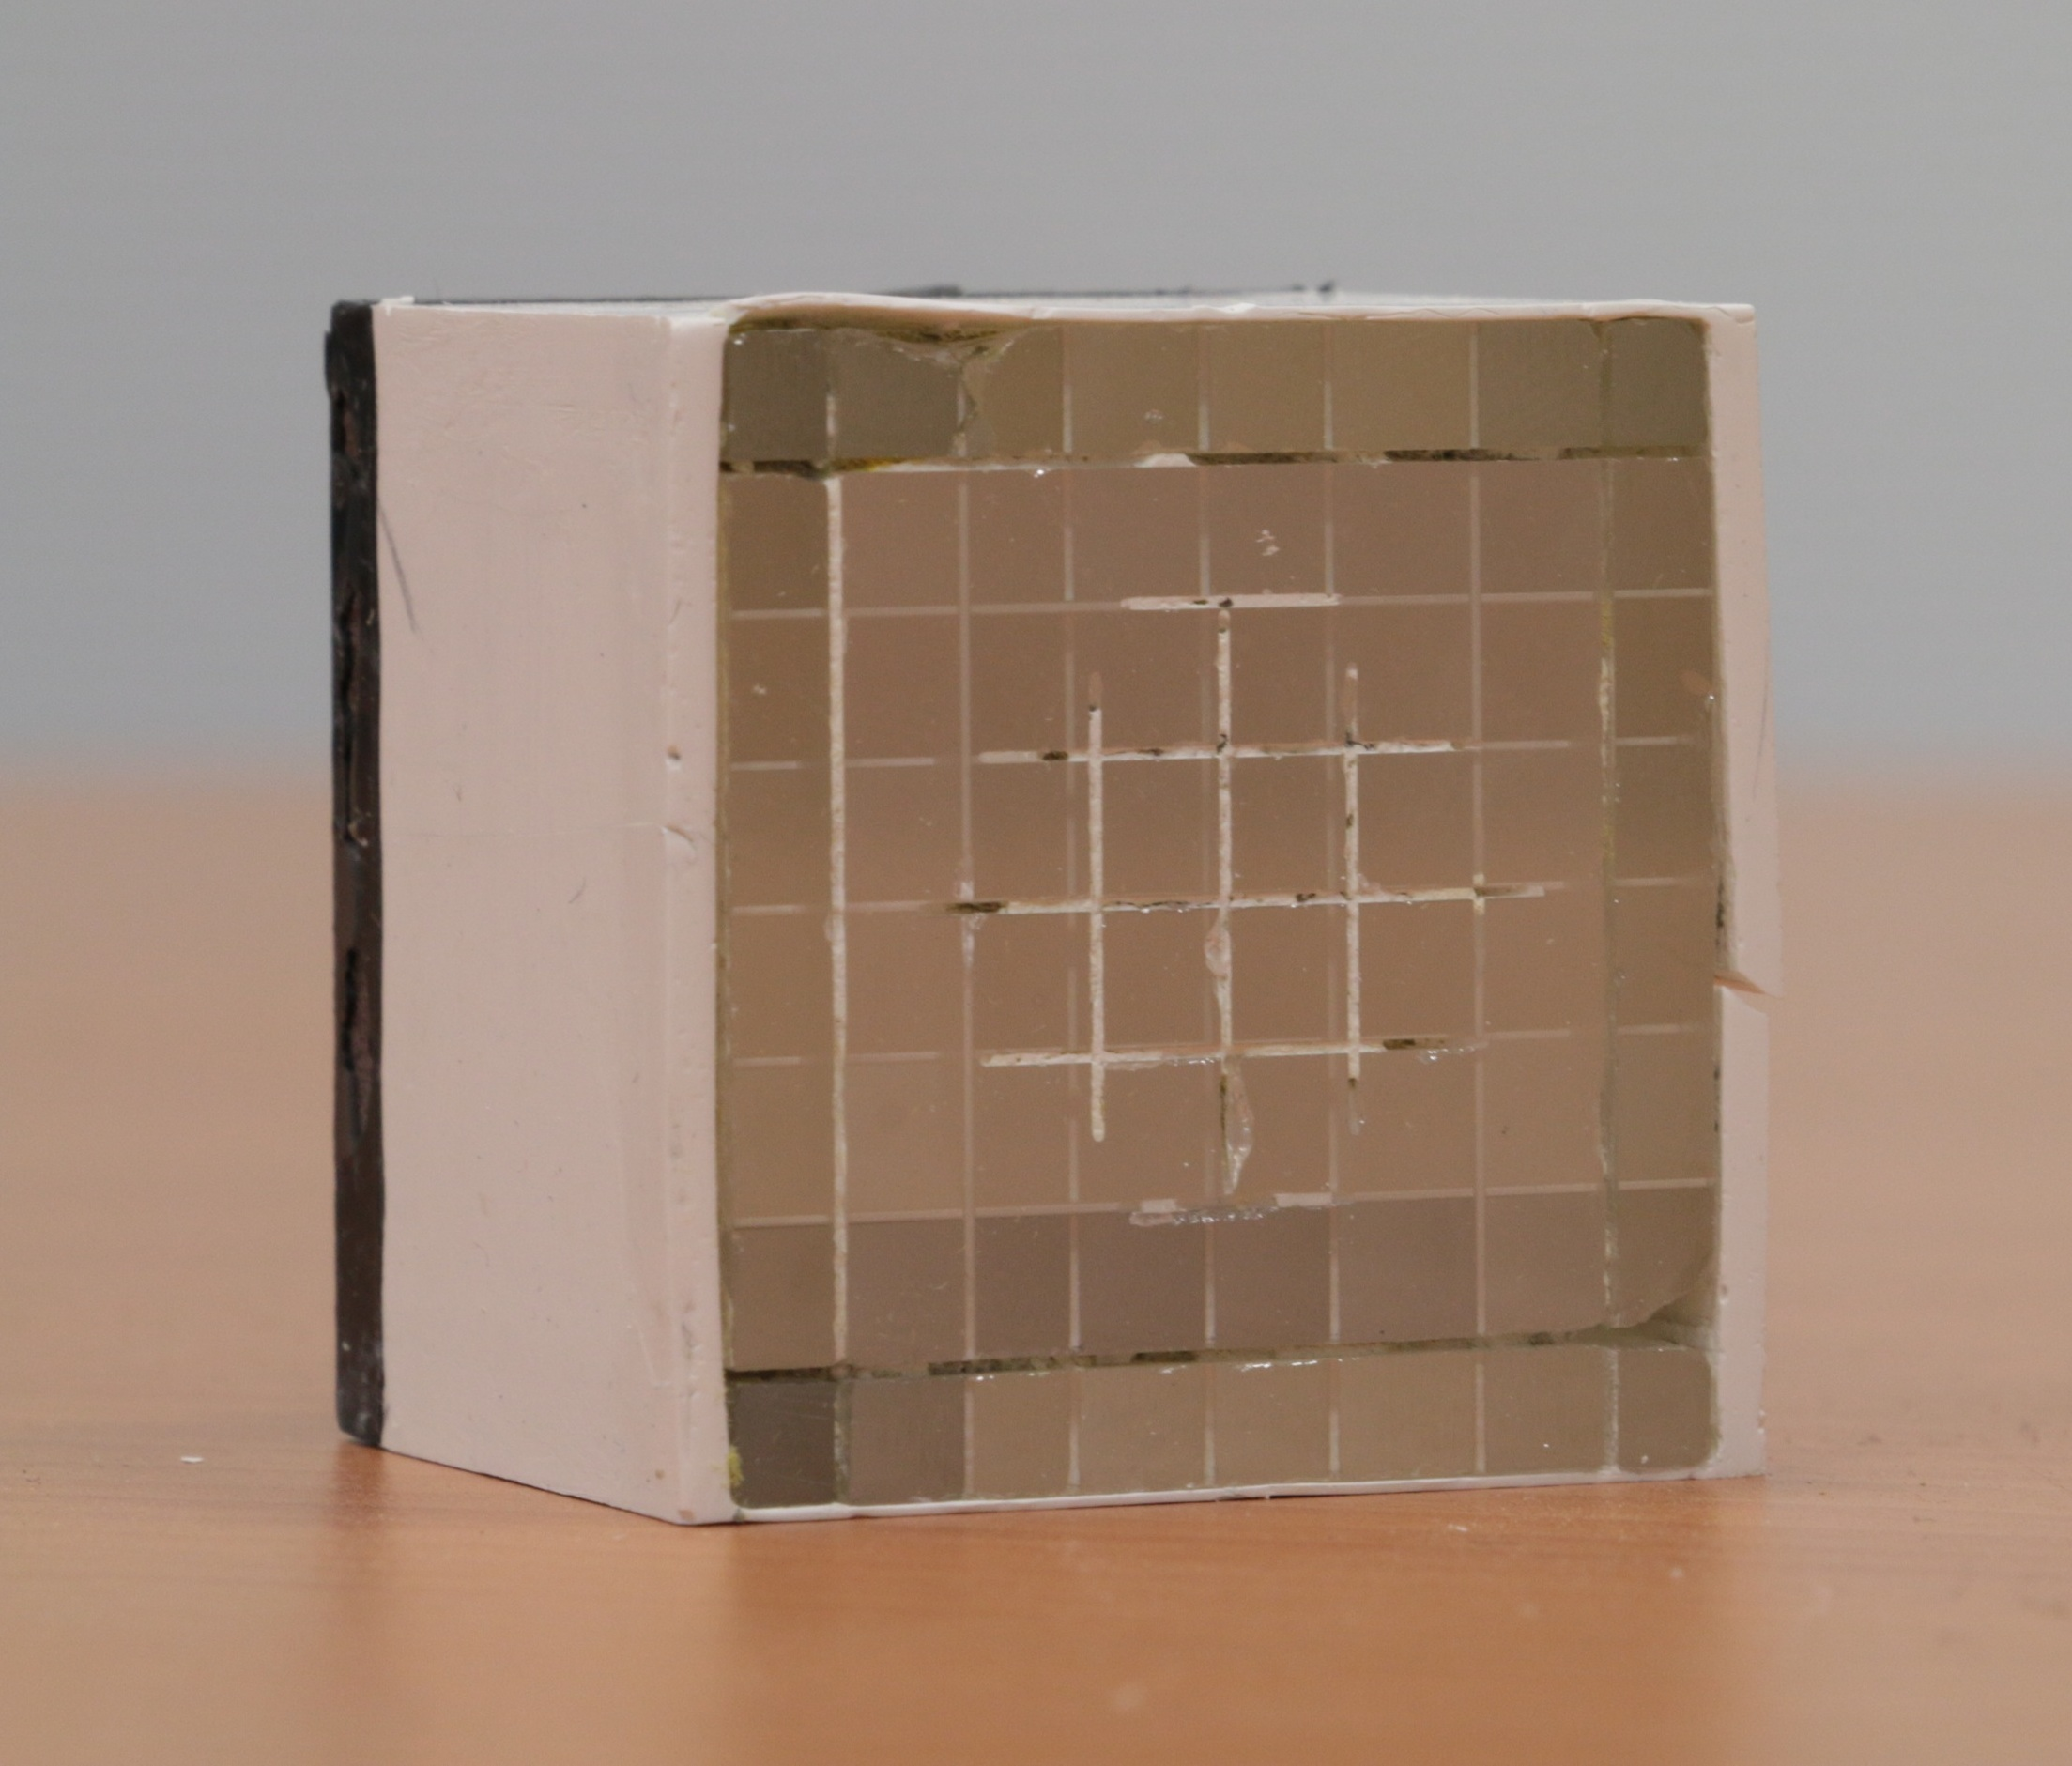
\includegraphics[width=1\textwidth, height=16em]{03_GraphicFiles/chapter3_CLaRySproto/Absorber/images/block_noPM}
\caption{\gls{bgo} block with its pseudo-pixel internal structure.}
\label{chap3::fig::block_noPM}
\end{subfigure}
\begin{subfigure}[t]{.5\textwidth}
\centering
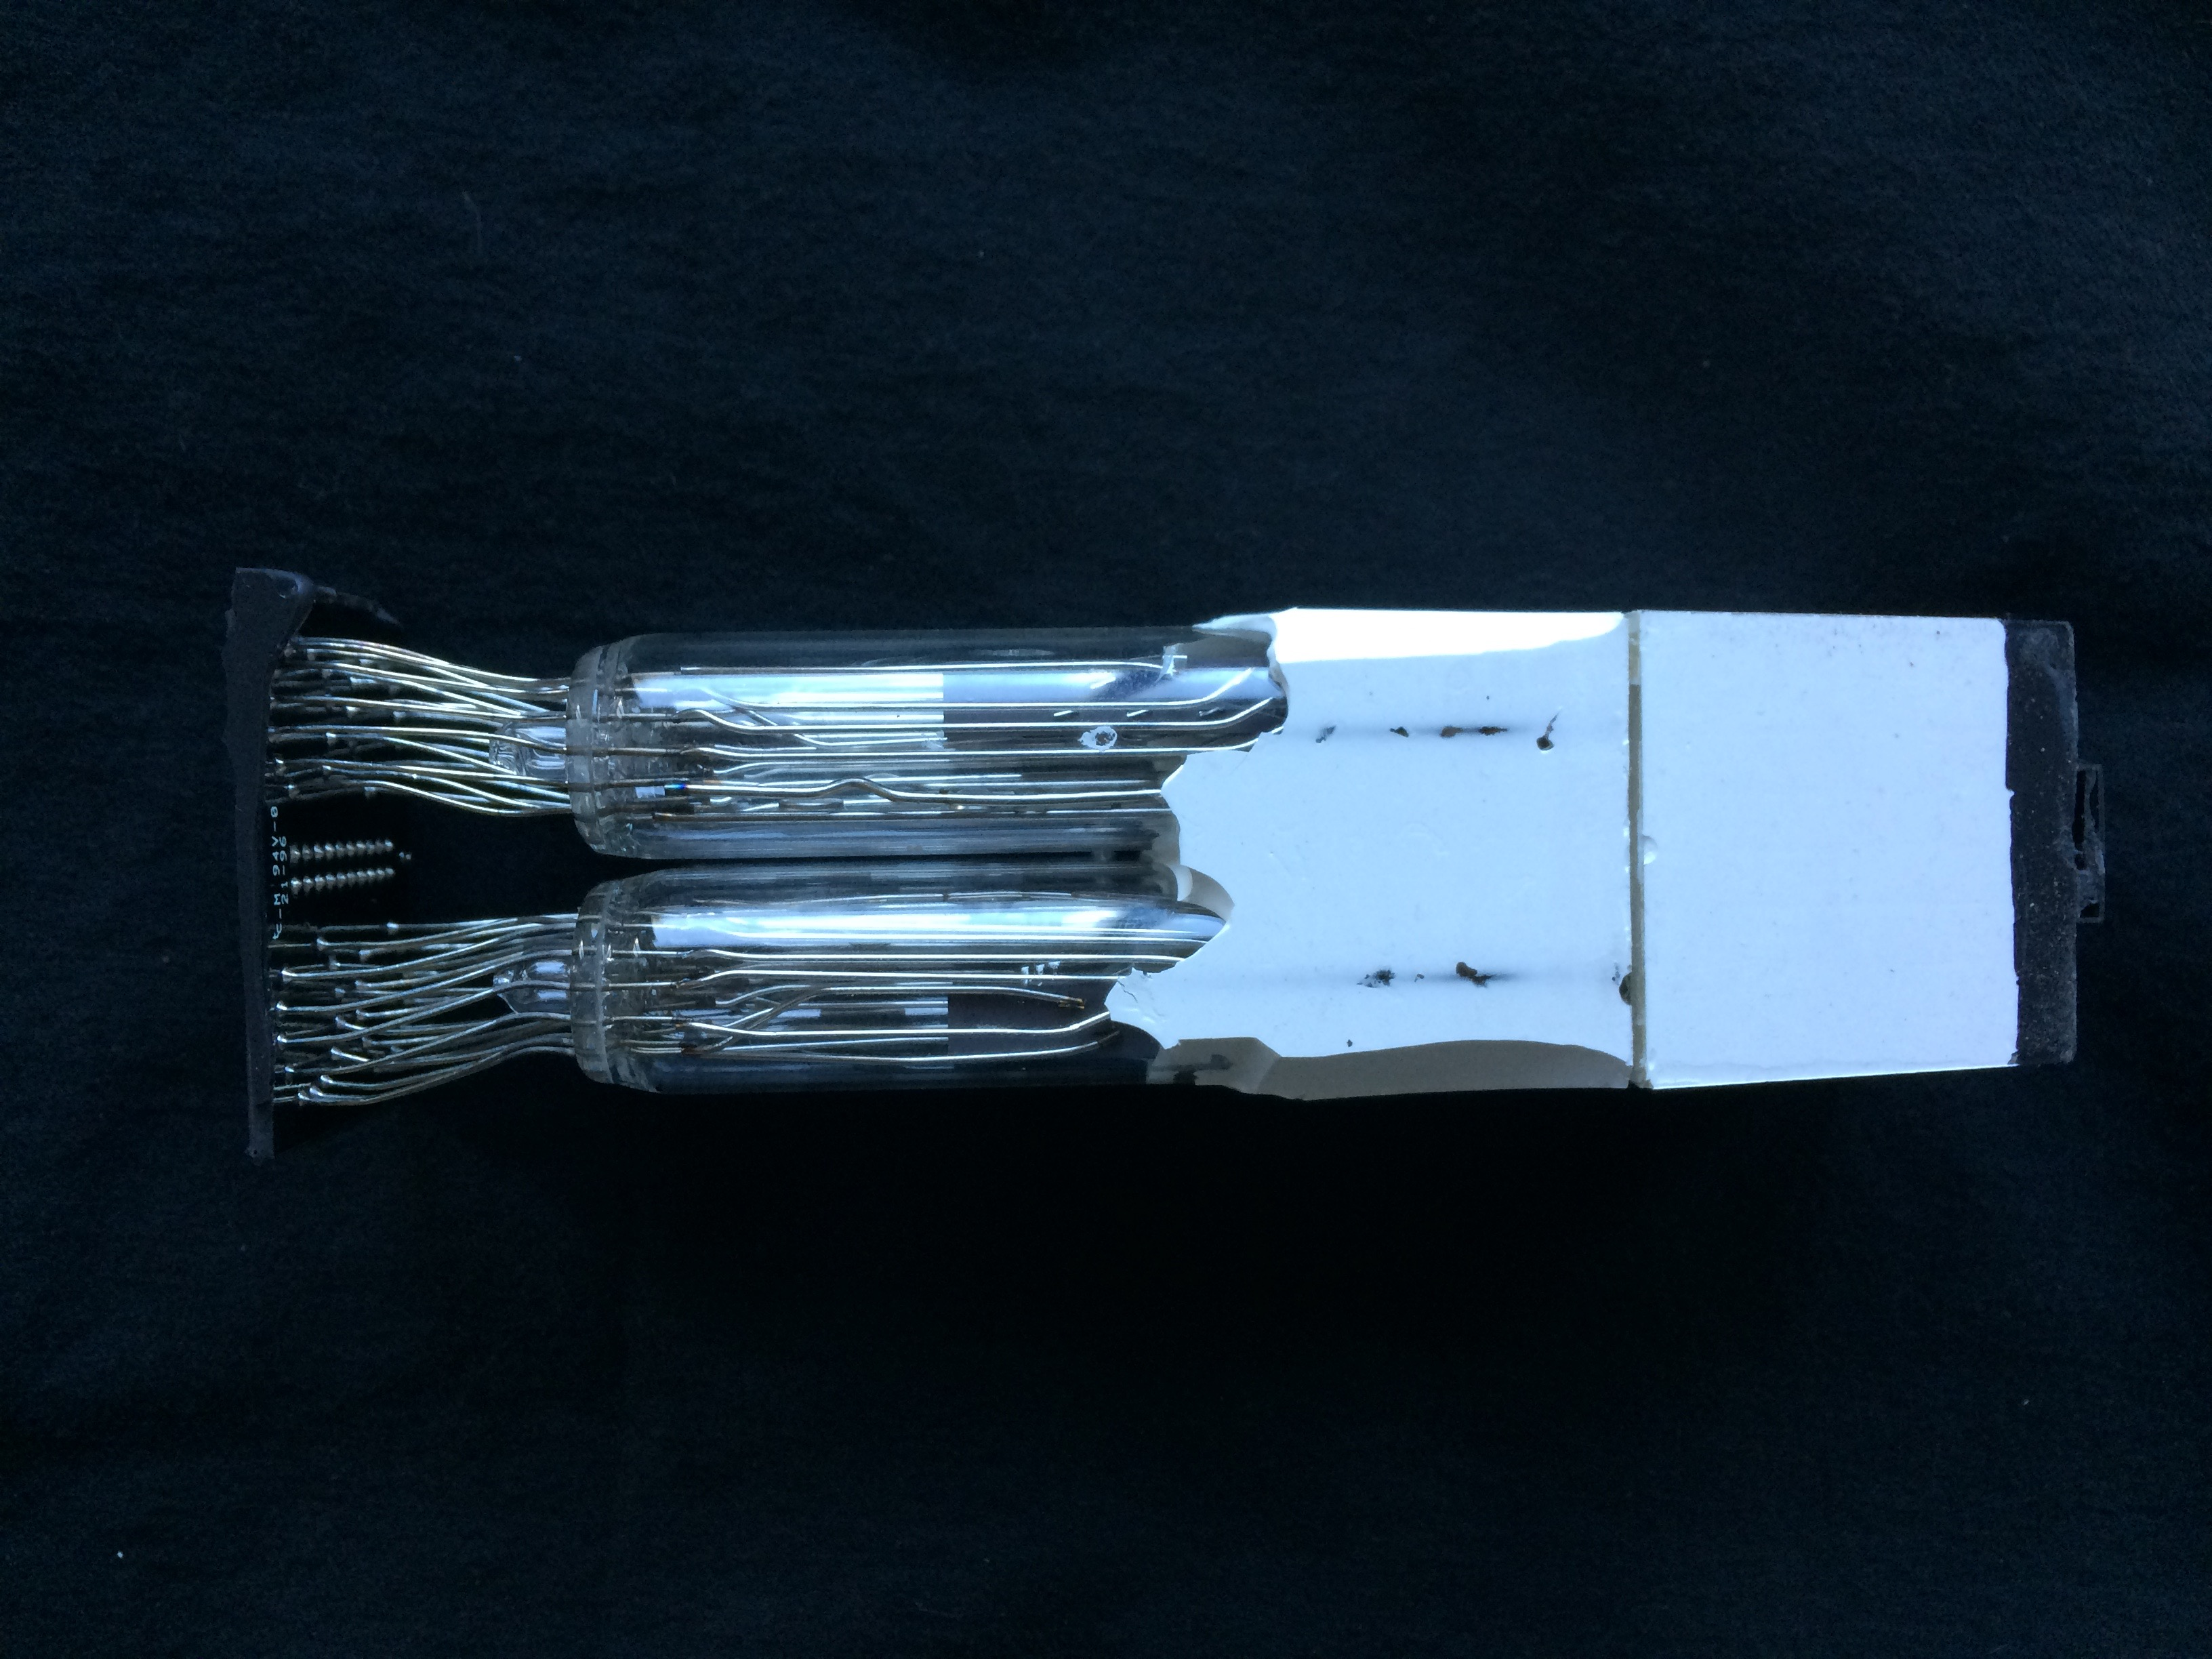
\includegraphics[width=1\textwidth, height=16em]{03_GraphicFiles/chapter3_CLaRySproto/Absorber/images/originalBlock_noAluminum}
\caption{\gls{bgo} crystal coupled to \gls{PM} quartet and covered with white reflecting material.}
\label{chap3::fig::originalBlock_noAl}
\end{subfigure}\newline
\begin{subfigure}[t]{.5\textwidth}
\centering
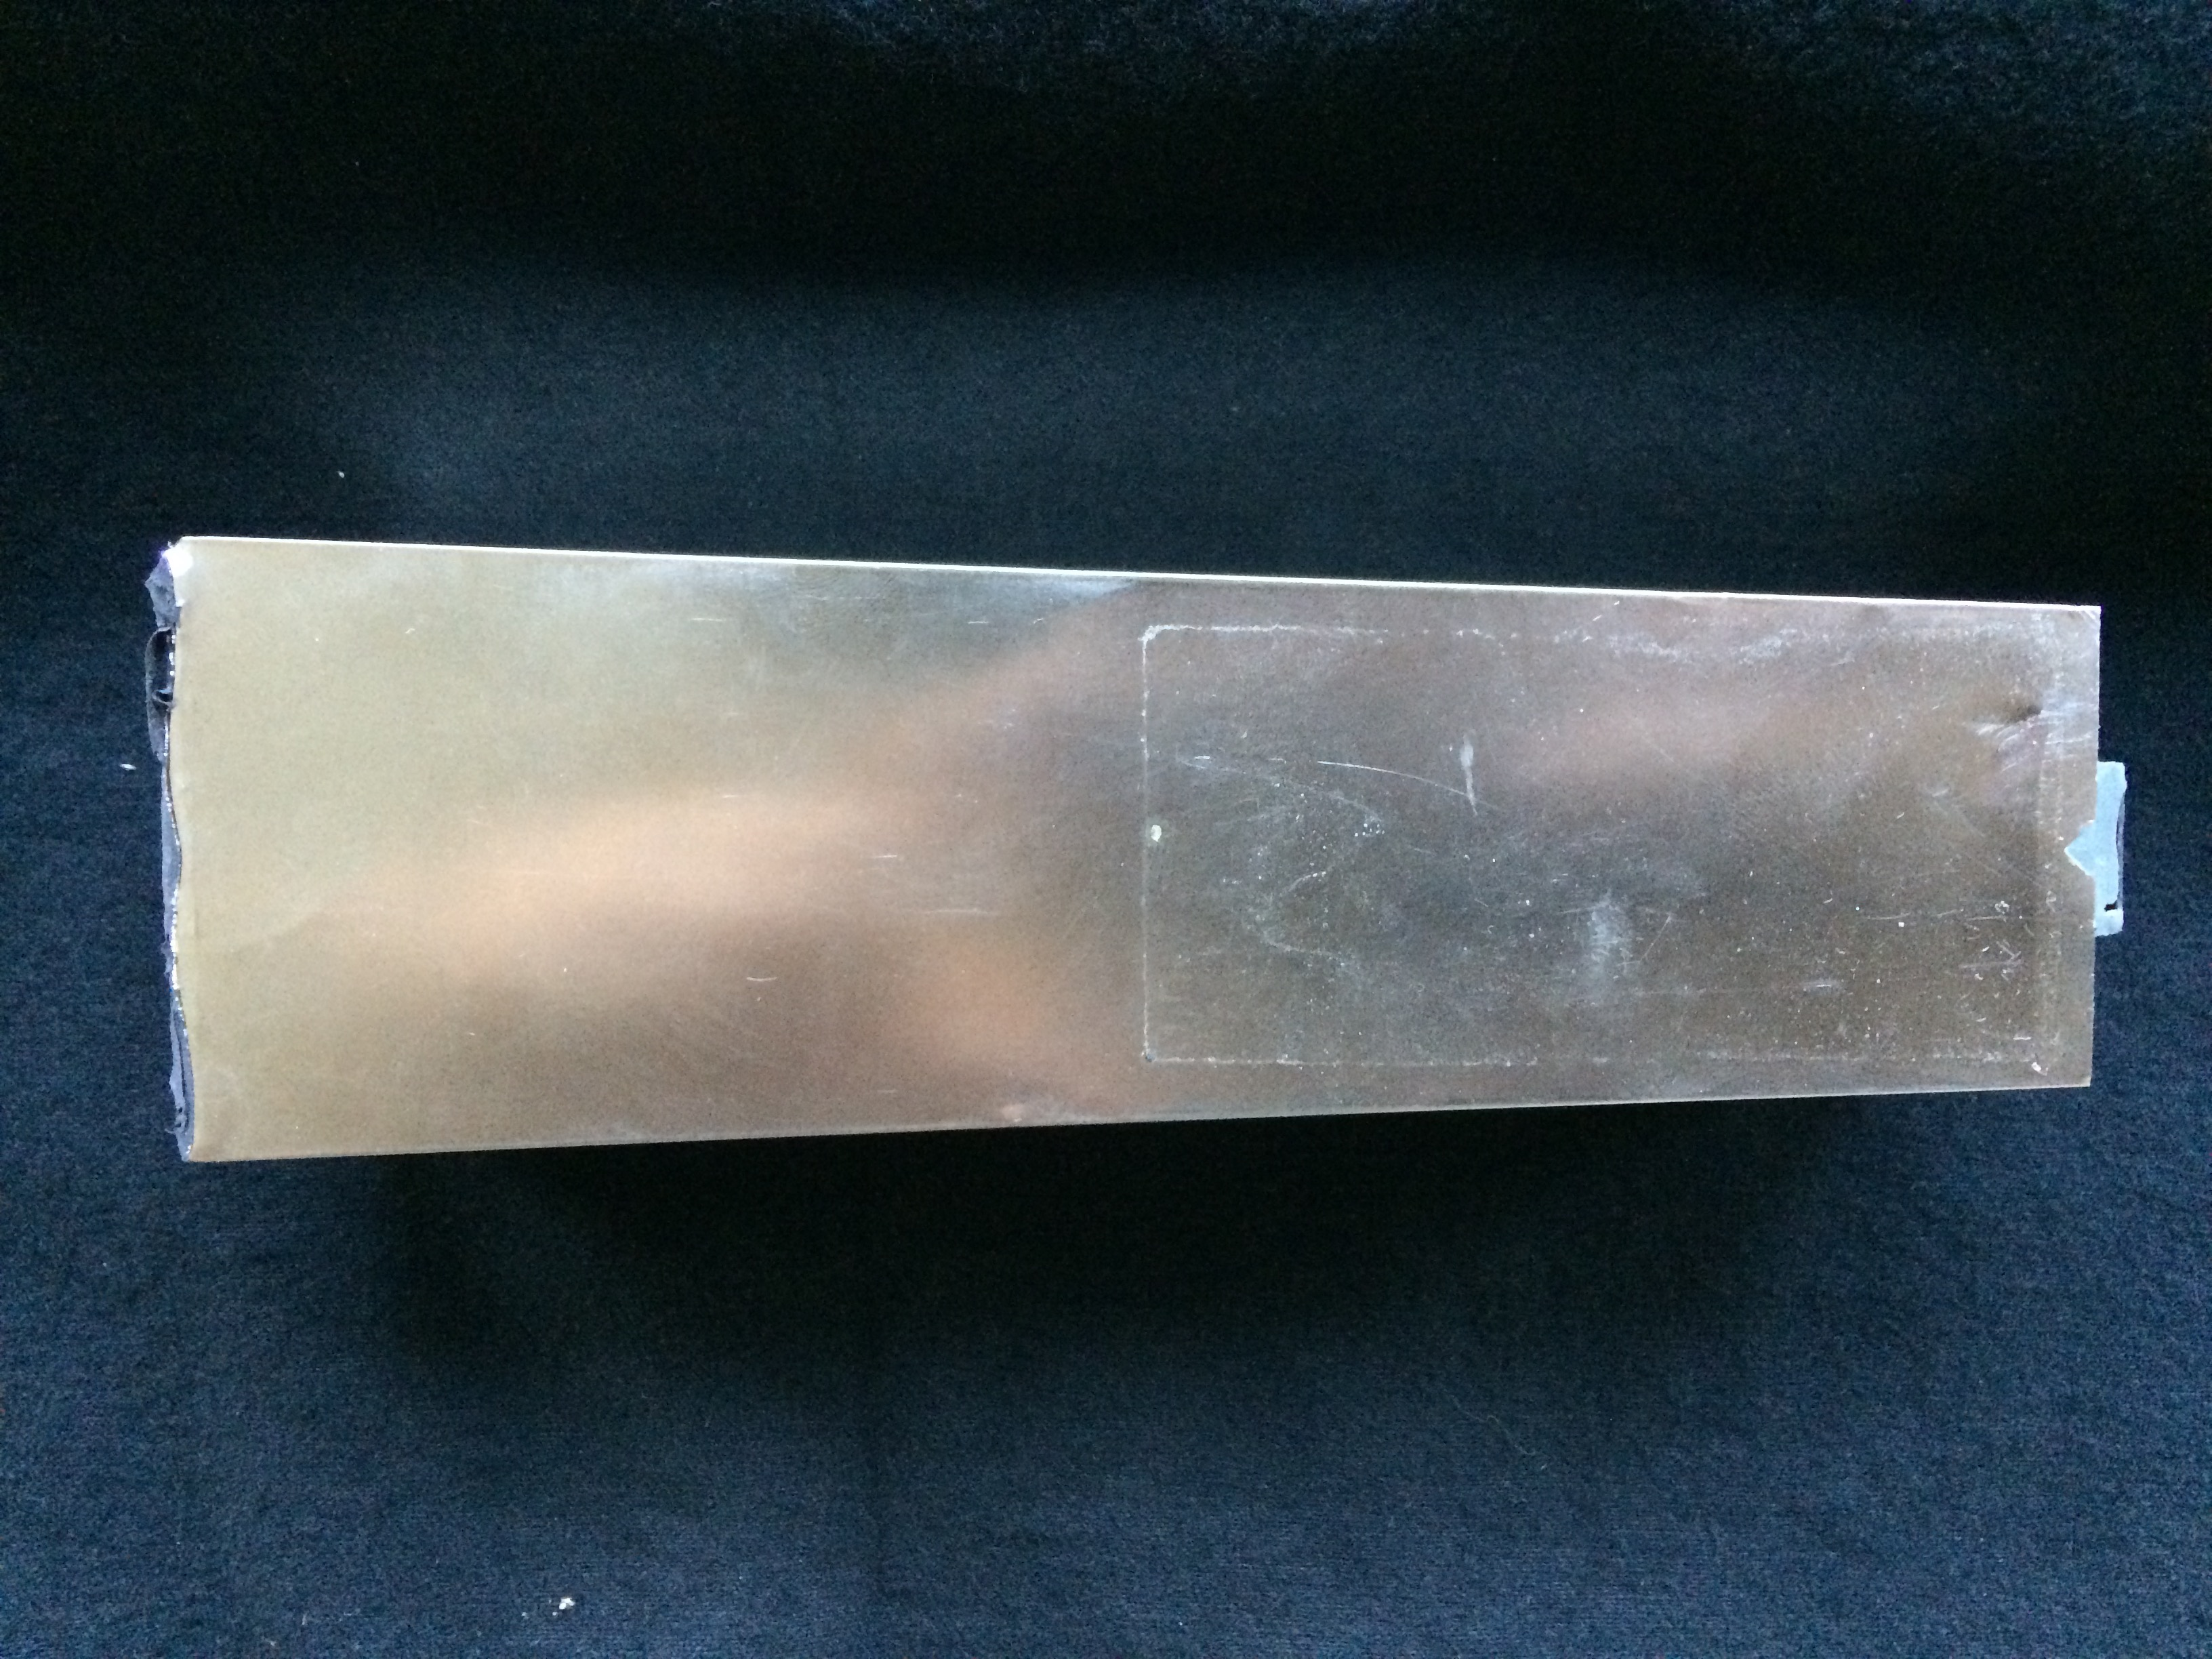
\includegraphics[width=1\textwidth, height=16em]{03_GraphicFiles/chapter3_CLaRySproto/Absorber/images/originalBlock_withAluminum}
\caption{\gls{bgo} complete module with aluminum cover.}
\label{chap3::fig::originalBlock_withAl}
\end{subfigure}
\begin{subfigure}[t]{.5\textwidth}
\centering
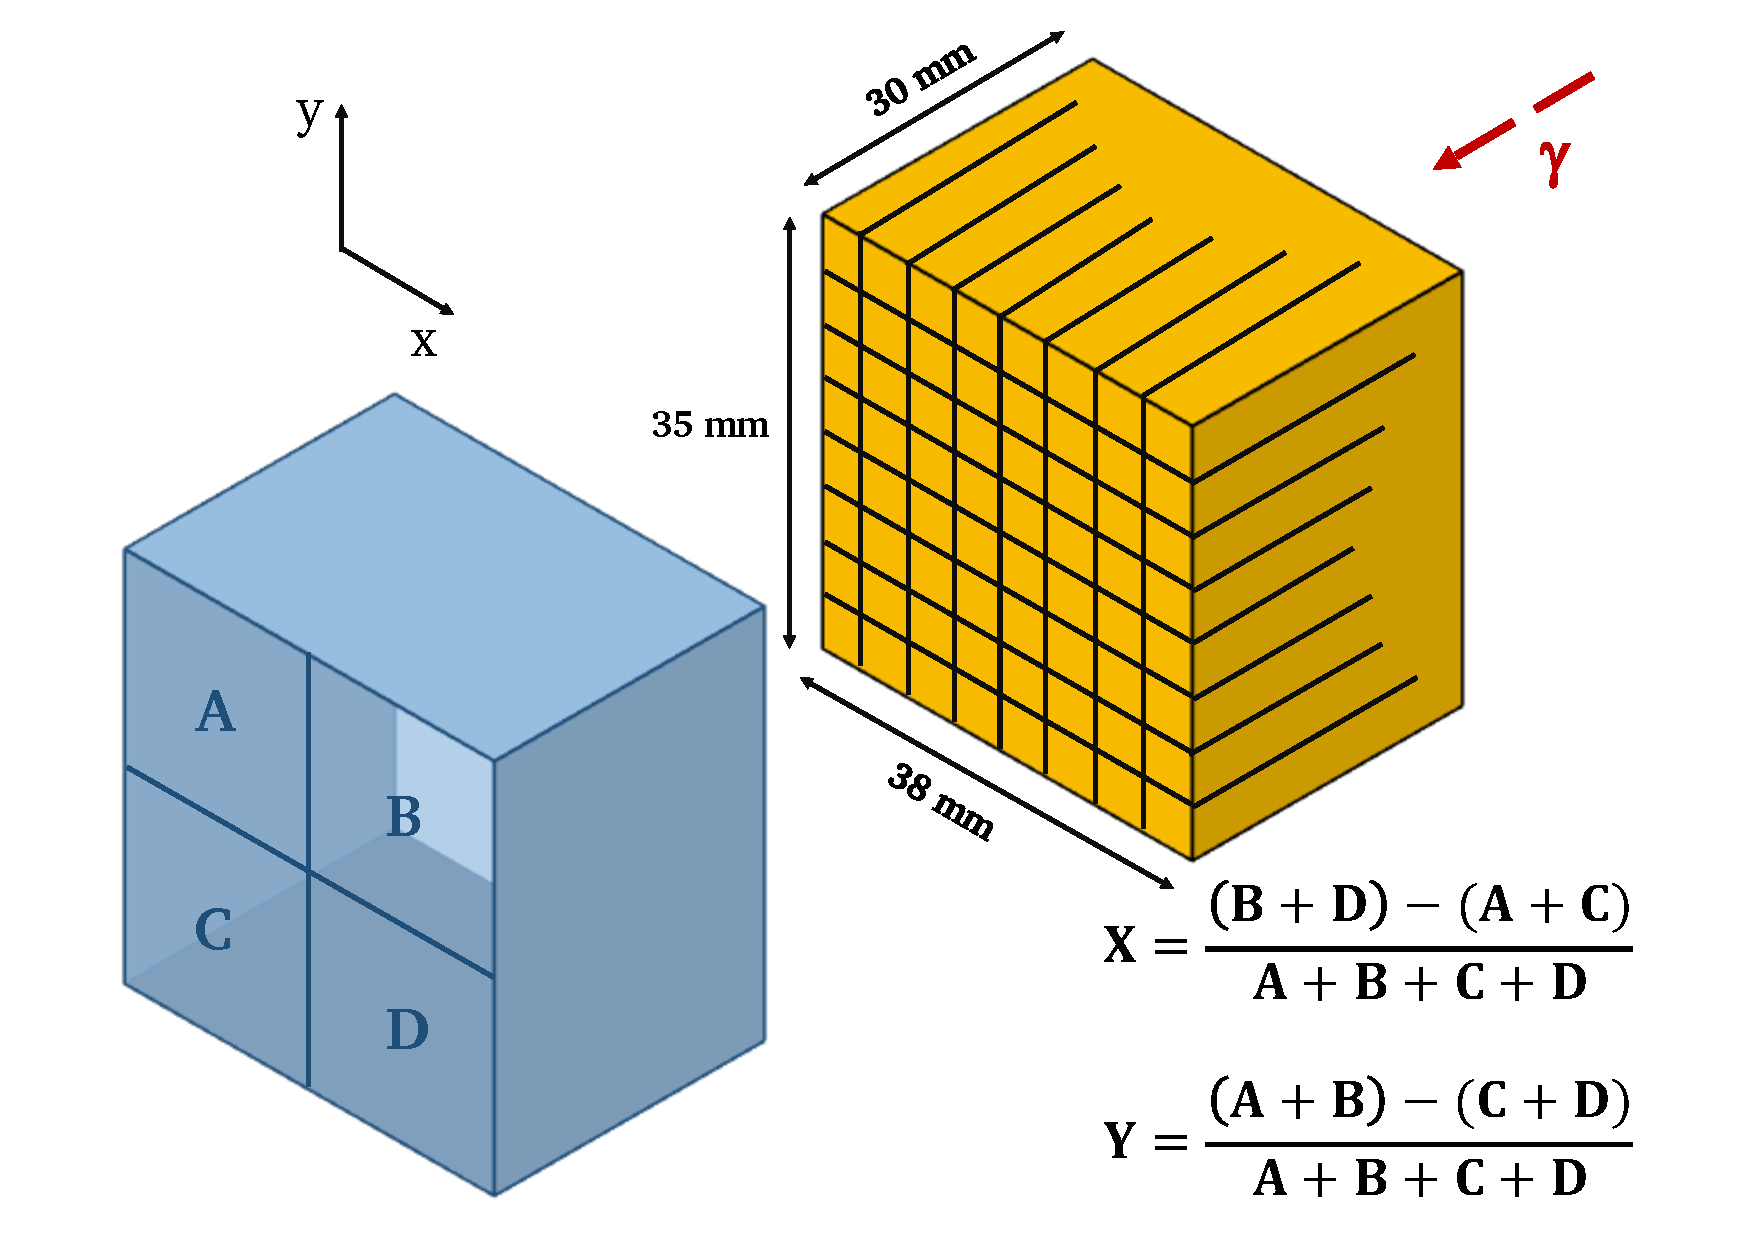
\includegraphics[width=1\textwidth, height=16em]{03_GraphicFiles/chapter3_CLaRySproto/Absorber/block_scheme.pdf}
\caption{Scheme of a \gls{bgo} block and its spatial reconstruction logic.}
\label{chap3::fig::BGOblockScheme} 
\end{subfigure}
\caption{Components of an absorber module and its working principle.}
\label{chap5::fig::BGO_block}
\end{figure}


\subsubsection{Absorber Front-End and read-out cards}\label{chap3::subsubsec::AbsorberFEcard}

A custom front-end card has been designed and produced by the \gls{lpc} research group \gls{avirm} and is used for the read-out of each \gls{bgo} block. The card is equipped with four voltage modulators which divide the provided high voltage on the 4 photo multiplier tubes. The voltage sent to each \gls{pm} can be mechanically tuned via screw-potentiometers on these modules. A $\varpm$~5~V low voltage is applied to the cards as supply for the differential amplifier modules, one per \gls{pm}. Differential output channels are used to send the \gls{pm} signals to the read-out card, called \gls{asm} board, via flat cables. A picture of the \gls{fe} card is given in \figurename~\ref{chap3::fig::FEcard}. To be noticed that four analog output channels has been added on some cards in order to allow laboratory tests with a signal treatment based on standard electronics modules, as described in section~\ref{chap3::sec::charMeasurements}. These outputs retrieve the signal before the differential amplification stage.\\ 

\begin{figure}
\begin{subfigure}[htbp]{0.5\textwidth}
\centering
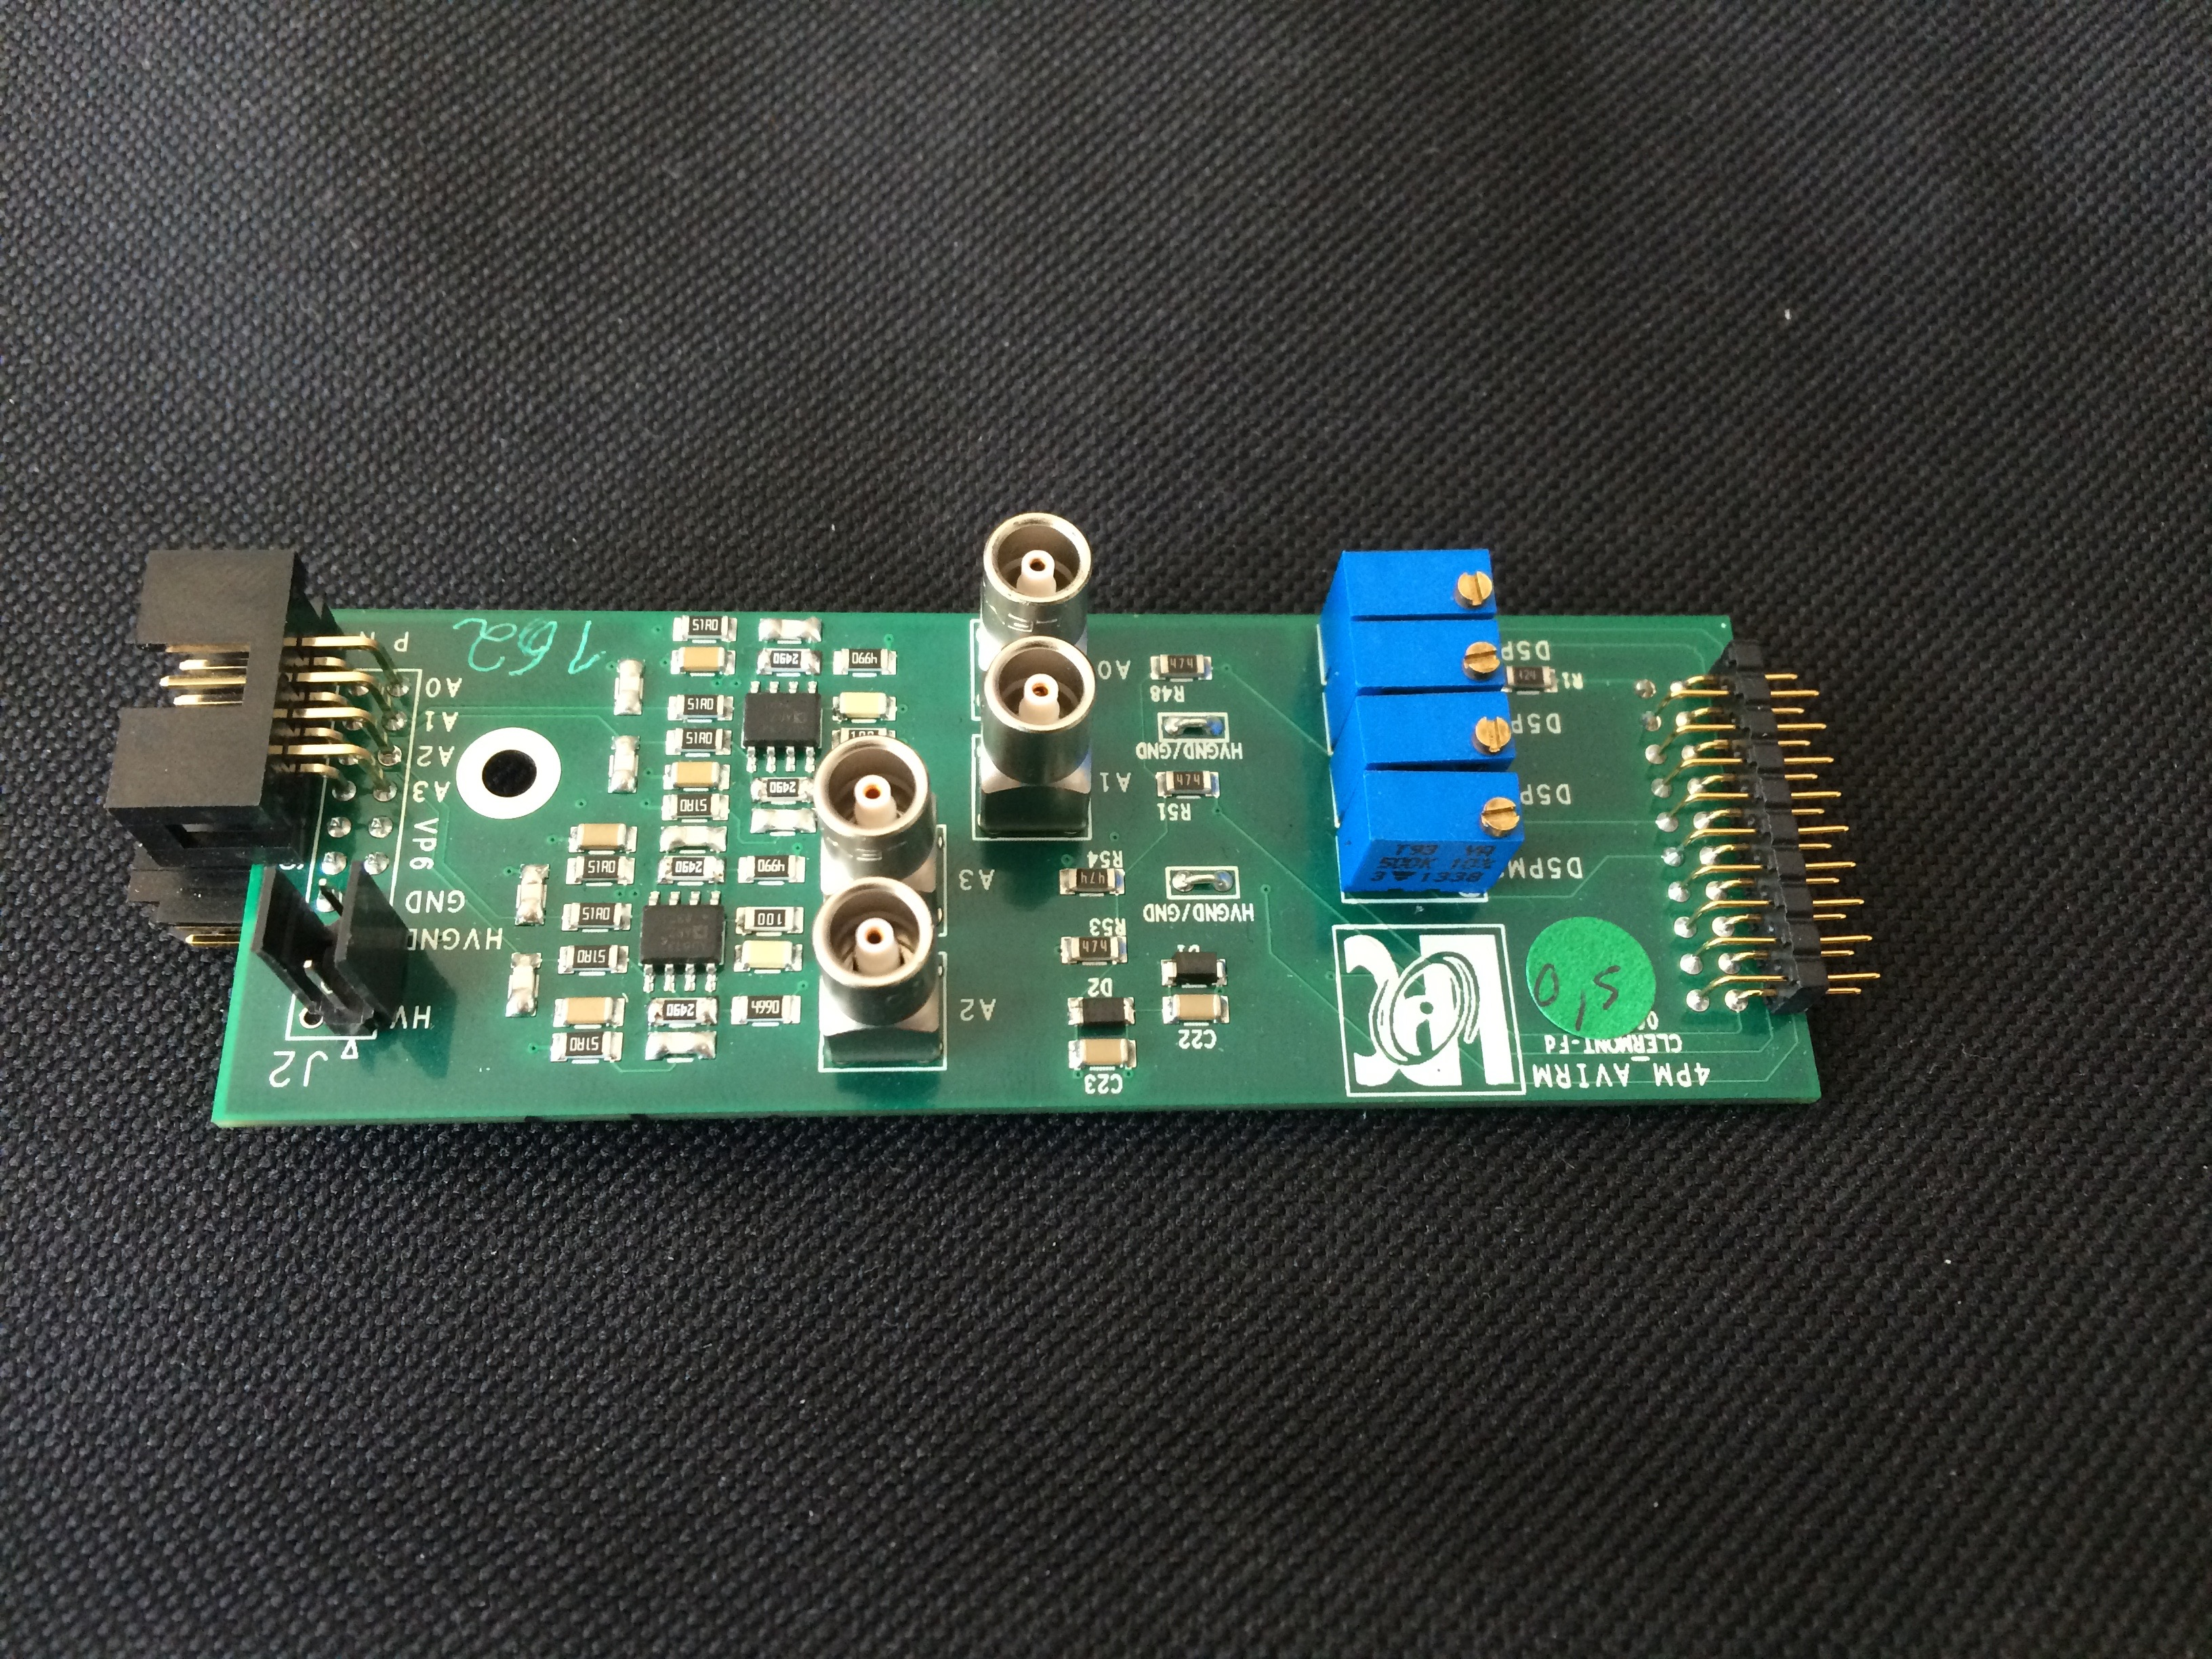
\includegraphics[width=\linewidth, angle = -90]{03_GraphicFiles/chapter3_CLaRySproto/Absorber/images/FEcard}
\caption{\gls{fe} card of the absorber \gls{bgo} detectors. 4 analog outputs have been added for test purpose.}
\label{chap3::fig::FEcard} 
\end{subfigure}
\begin{subfigure}[htbp]{0.5\textwidth}
\centering
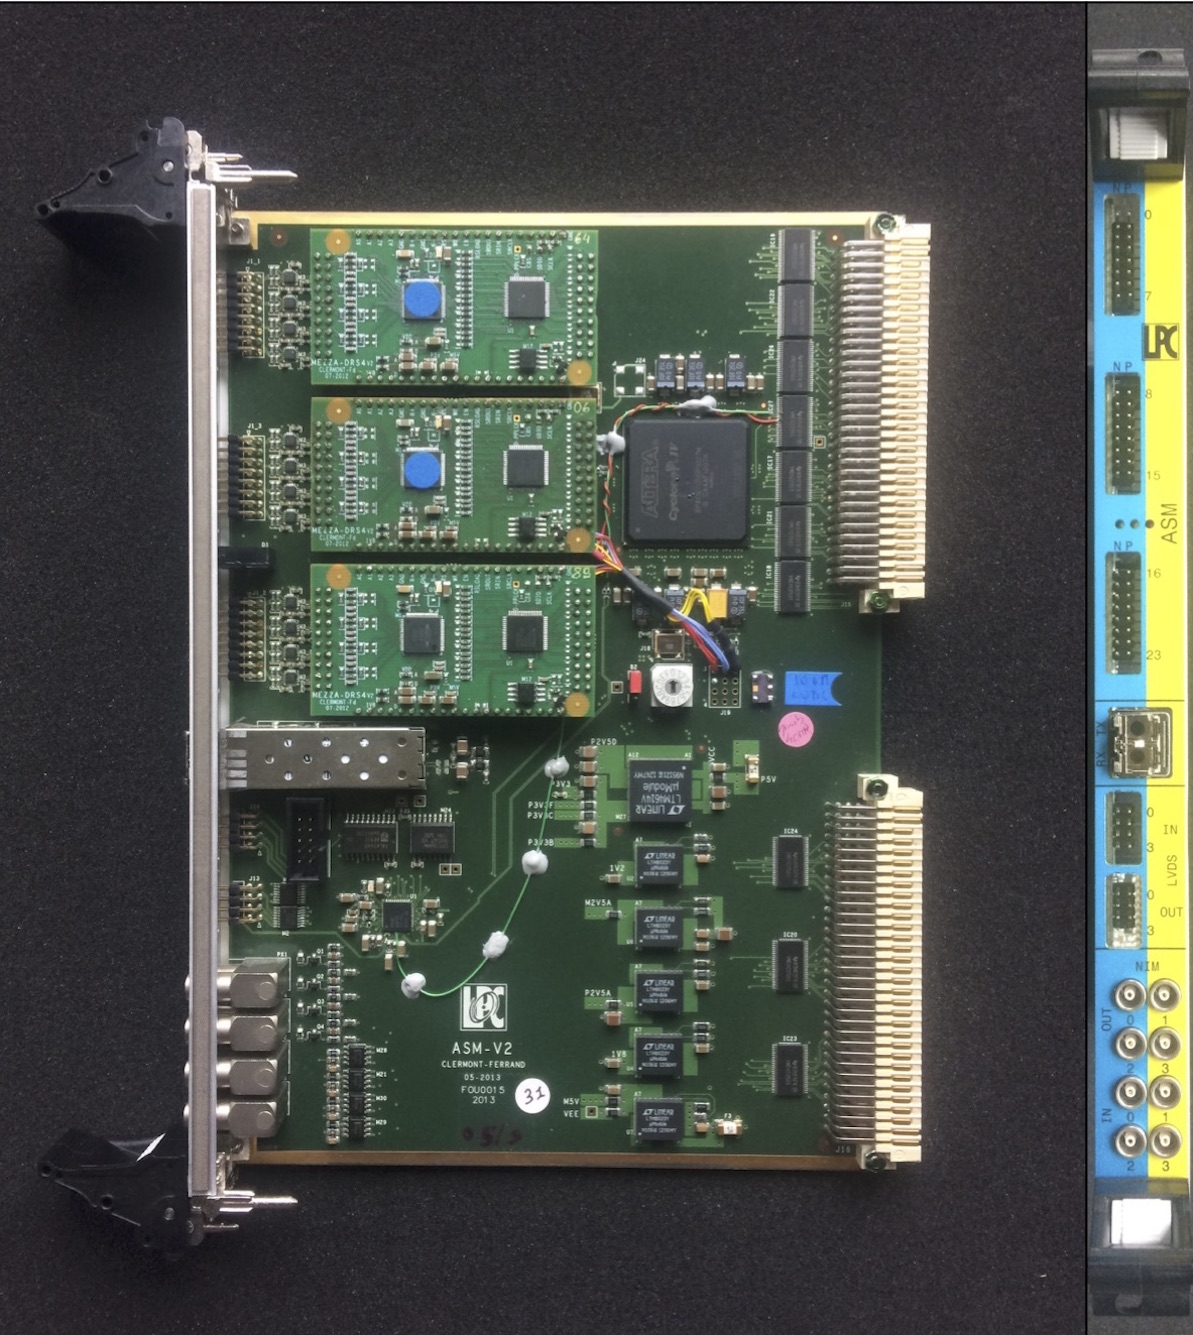
\includegraphics[width=0.89\linewidth,]{03_GraphicFiles/chapter3_CLaRySproto/Absorber/ASMcard.jpg}
\caption{\gls{asm} board of the absorber \gls{bgo} detectors. Each board performs the read-out of 6 blocks.}
\label{chap3::fig::ASMcard} 
\end{subfigure}
\caption{Absorber read-out electronics: \gls{fe} card (a) and \gls{asm} board (b).}
\label{chap5::fig::AbsorberCards}
\end{figure}

The \gls{pm} signals amplified by the \gls{fe} card are received by the \gls{asm} boards. Developed by the \gls{lpc} \gls{avirm} group, it is based on the \gls{vme} standard and designed for the application in the \gls{dpga} \gls{pet} system, equipped with \gls{lyso} mono-crystals, grouped in quartets and read-out by the same \gls{fe} card described above. The adaptation to the gamma camera application, so that for the \gls{bgo} modules signal treatment, involves only the firmware part, while the design of the board is unchanged. Each board has 24 differential inputs and it is so able to read the signals from 6 \gls{bgo} blocks; a total of 5 boards are then needed for the complete read-out of the gamma camera absorber (30 blocks). The incoming signals are treated by three intermediate cards  equipped with a \gls{drs}4 chip~\parencite{Ritt2009}, designed and developed at the \gls{psi}, with 8 sampling channels at a maximum frequency of 5~\gls{gsps} (200~ps) for 1024 samples, and an \gls{adc} 12~bit-20~MHz module. The sampling frequency of the \gls{drs}4 can be modified to fit with the specific application: in particular, the \gls{bgo} blocks produces wider signals with respect to the \gls{lyso} crystals of the \gls{dpga}. A \gls{fpga} Altera Cyclone IV GX~\parencite{Altera2016} receives and handles the digital outputs of the three intermediate cards and is in charge of sending the date to the acquisition system via a 3~Gbit/s optical link. The \gls{fpga} also governs the generation of the pre-trigger signal which is sent to an auxiliary board called \gls{thor} in order to start the acquisition of the gamma cameras, as detailed in section~\ref{chap3::subsec::cameraElectronicsDAQ}.\\

\underline{Absorber acquisition with development card} \\

During the development of the final camera acquisition system based on the \gls{utca} equipment, which required a dedicated firmware development ad testing process, a temporary acquisition system has been set for the absorber \gls{bgo} blocks, mainly dedicated to the test and characterization of the \gls{asm} boards. It is based on a development commercial electronics card, provided by Terasic (Altera University Program), equipped with an \gls{fpga} Altera Cyclone V~\parencite{Terasic2015}. The card \gls{fpga} can be programmed for the needed tasks, and it is directly connected to an acquisition PC via Ethernet cable. Three \gls{hsmc} connectors allows for the connection to an expansion board SFP-HSMC~\parencite{Terasic2009}, again by Terasic (Altera University Program), provided with a second \gls{fpga} and with optical fiber input/output connectors for the interface to the \gls{asm} boards. A single optical input is configured for this acquisition setup, with the firmware developed by the \gls{avirm} group in \gls{lpc} and adapted at the \gls{ipnl}; one single \gls{asm} card can be connected to the board, so that a maximum of 6 \gls{bgo} block can be read-out at the same time. A picture of the development card connected to the mezzanine is given in \figurename~\ref{chap3::fig::absDevelcard}. \figurename~\ref{chap3::fig::softDevelCard} shows an example of the user interface and data visualization of the C++ based acquisition software developed and provided byt the \gls{avirm} group.   

\begin{figure}
\begin{subfigure}[htbp]{0.5\textwidth}
\centering
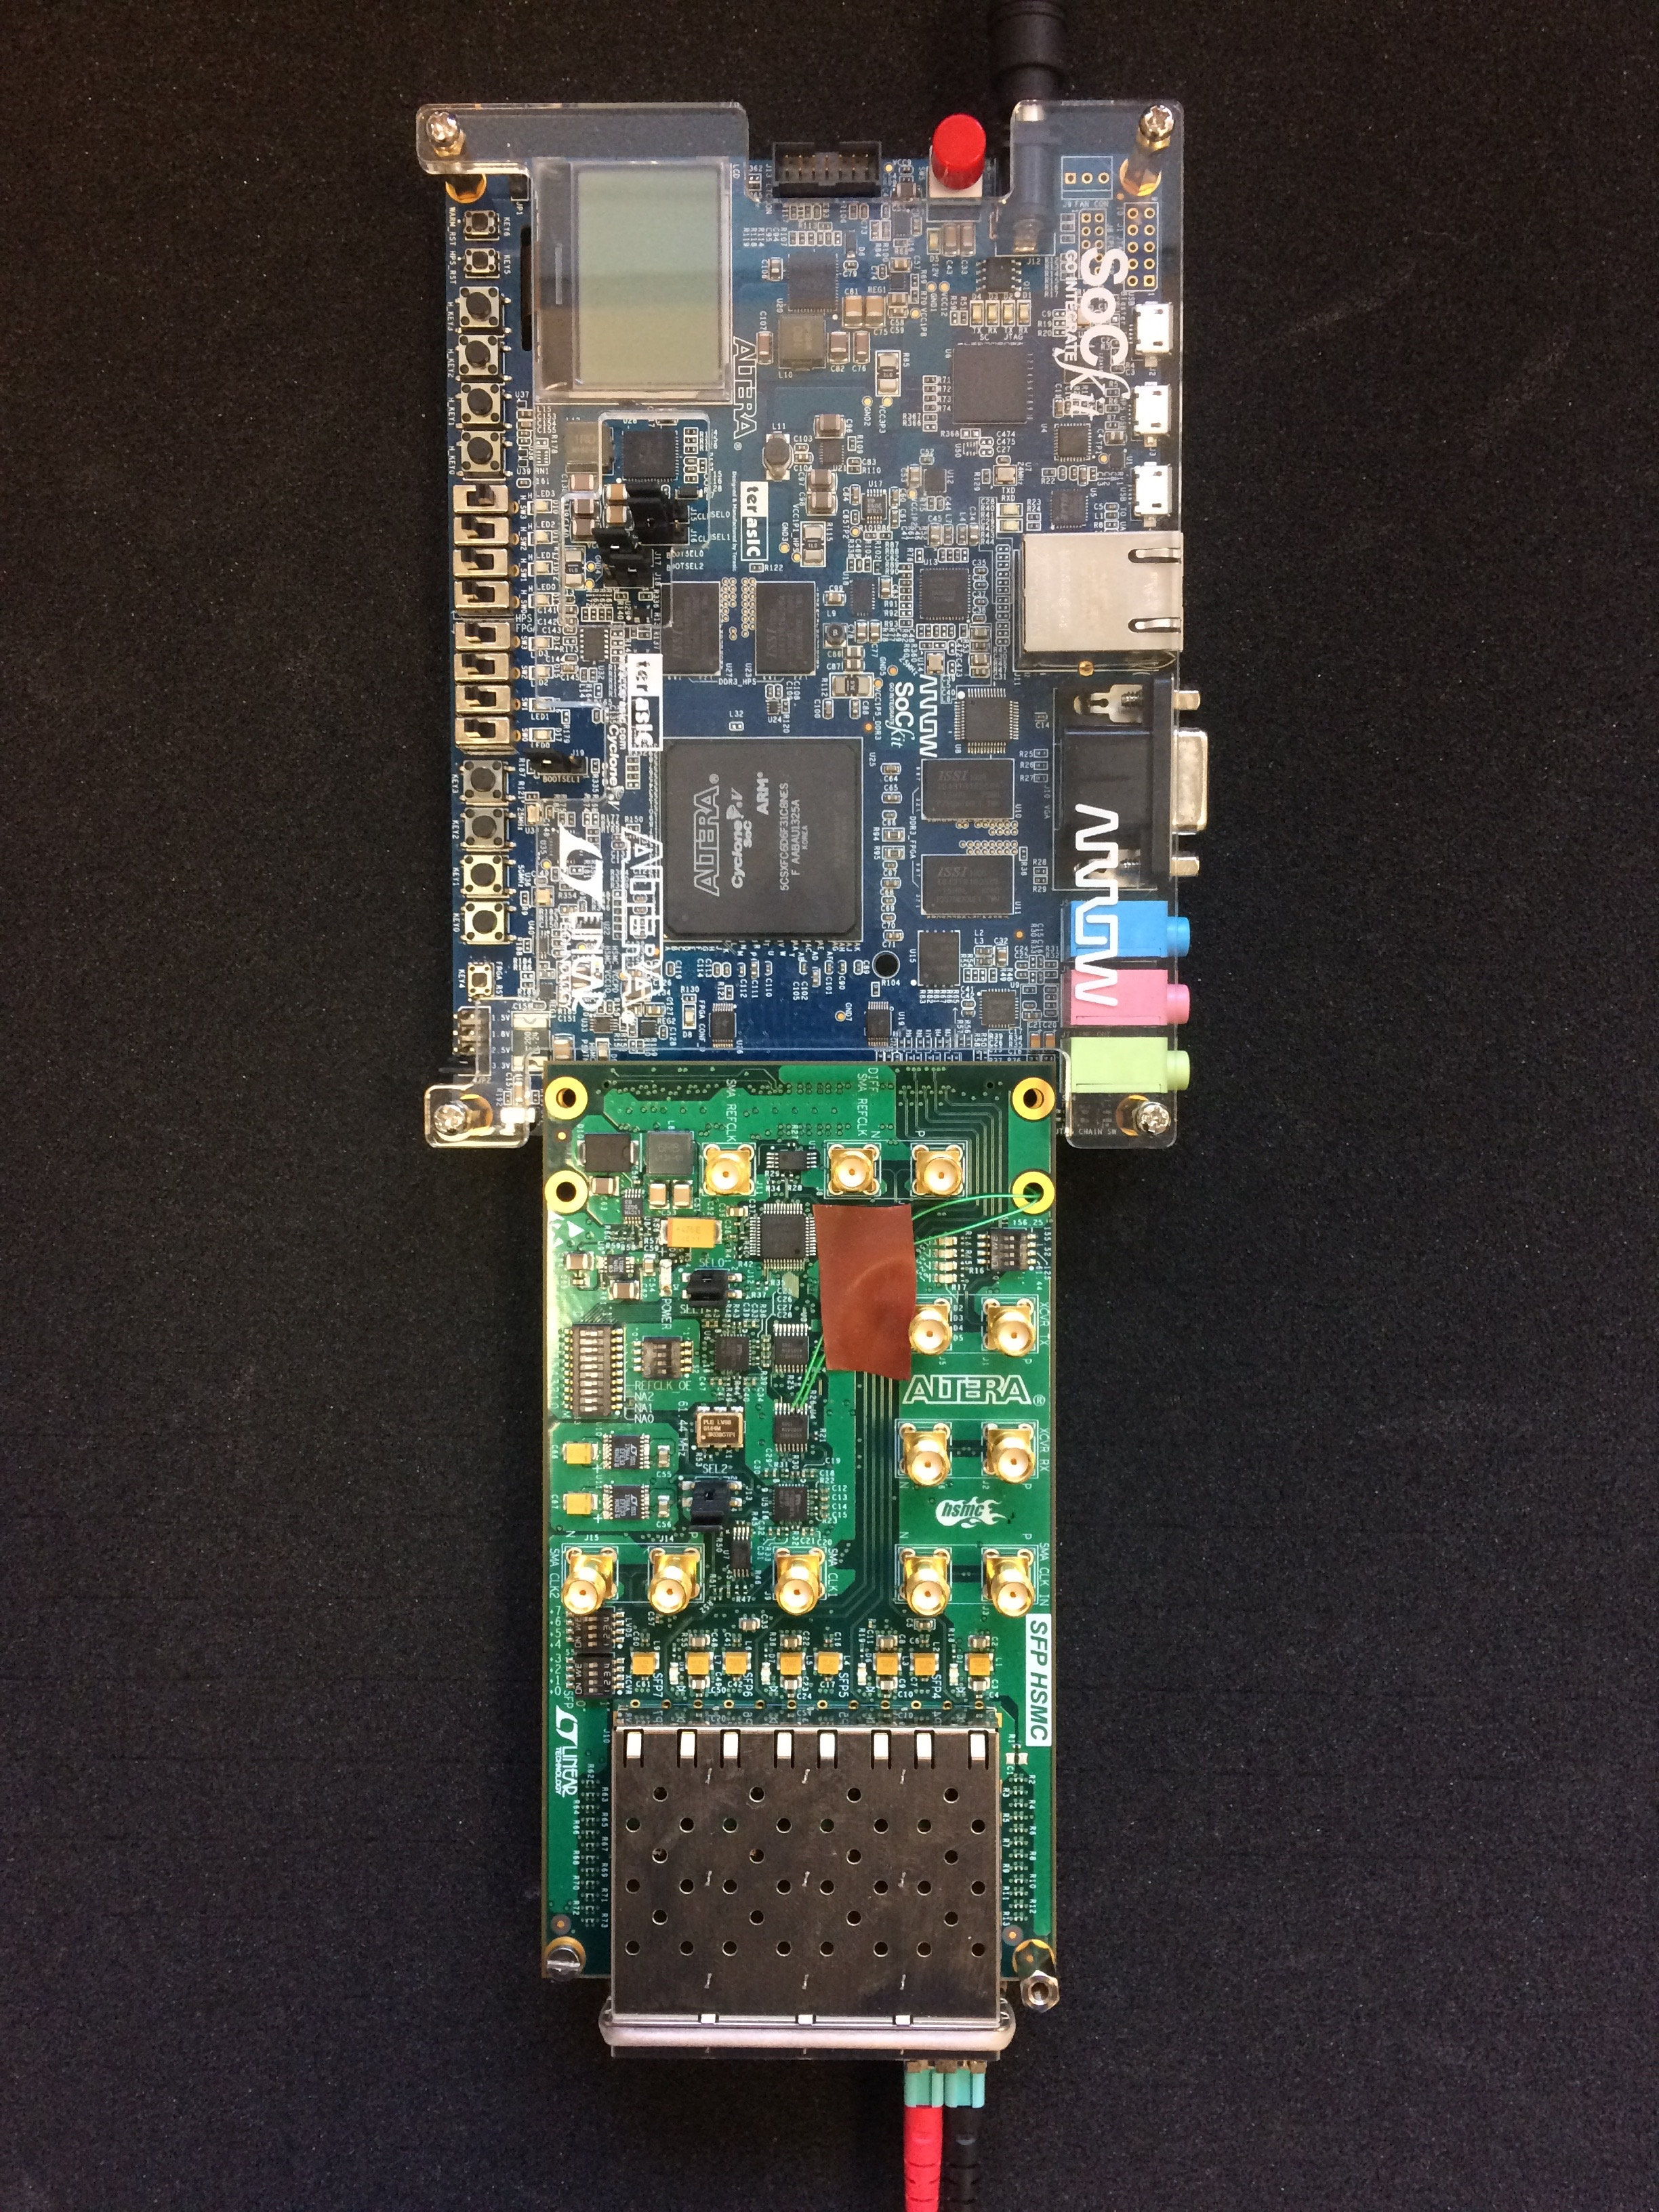
\includegraphics[width=0.75\linewidth, angle = 90]{03_GraphicFiles/chapter3_CLaRySproto/Absorber/develCard_zoom.jpg}
\caption{Altera development card for the absorber \gls{bgo} detectors.}
\label{chap3::fig::absDevelcard} 
\end{subfigure}
\begin{subfigure}[htbp]{0.5\textwidth}
\centering
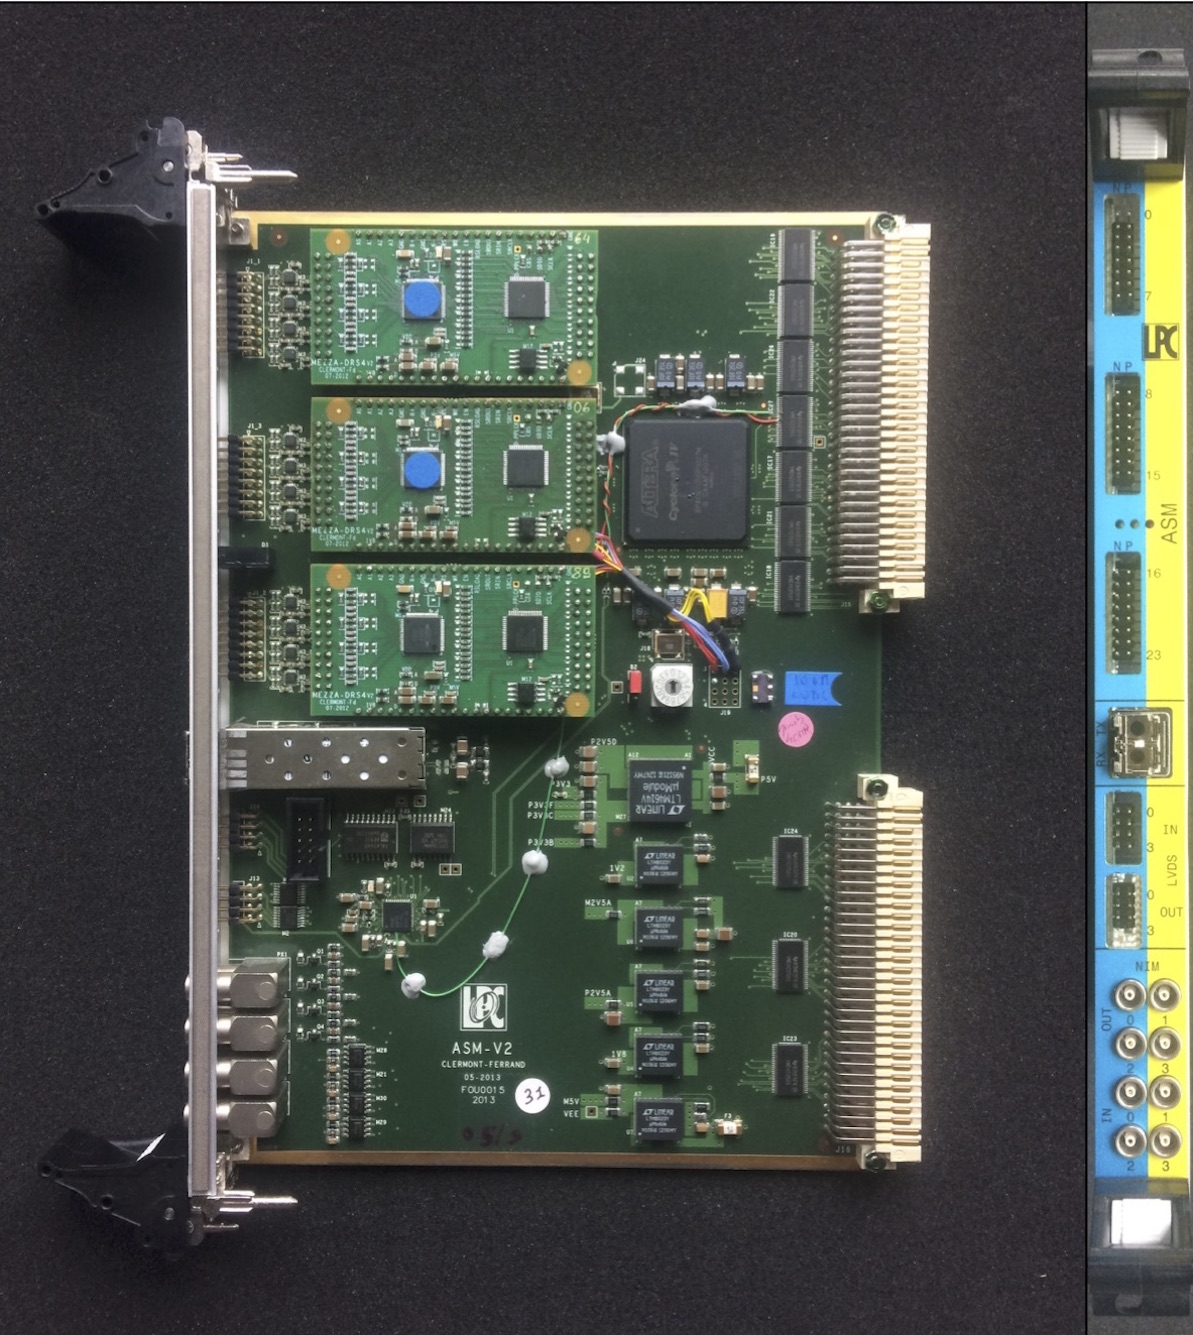
\includegraphics[width=\linewidth]{03_GraphicFiles/chapter3_CLaRySproto/Absorber/ASMcard.jpg}
\caption{Example of acquisition software interface for the absorber \gls{asm} card acquisition base on the Altera development card.}
\label{chap3::fig::softDevelCard} 
\end{subfigure}
\caption{Details of the temporary absorber acquisition based on the Altera development card.}
\label{chap5::fig::AbsorberDevelCards}
\end{figure}

\subsubsection{Absorber mechanical support}\label{chap3::subsubsec::AbsorberMechanics}

A first mechanical structure for the absorber detector was initially conceived by the \gls{lpc} group in order to hold up to 100 modules, foreseen by the original camera design. The reduction of the number of available blocks caused by the \enquote{reconditioning} process failure make necessary an adaptation of such a support. The new design has been carried out by the mechanics group of the \gls{ipnl} in order to be compact and flexible in terms of detection modules setup. \figurename~\ref{chap3::fig::absorber_scheme} displays both a picture and a scheme of the absorber configuration with its mechanical support. The two lateral sides are built with \gls{pmma} boards connected by metal bars, and the \gls{bgo} blocks can be arranged in up to 5 rows of variable size, ranging from 3 to 7 blocks. Each block row is supported by a thin metal foil, designed to reduce at minimum the blocks separation and to respect the original ring geometry deriving from the SIEMENS \gls{pet} system. The blocks composing a row are then laterally pressed via two screws on the two sides of the structure, which can also be used to adapt the rows relative position horizontally. On the back side, a metal bar is added to avoid undesired movements, and the \gls{fe} cards are fixed with plastic pillars. The realized support results to be versatile, compact and adapted to the prototype tests for both the Compton camera (where a squared setup is preferred) and the multi-collimated one (where the collimator geometry must be fit by the absorber geometrical configuration).       

\begin{figure}
\begin{subfigure}[b]{.5\textwidth}
\centering
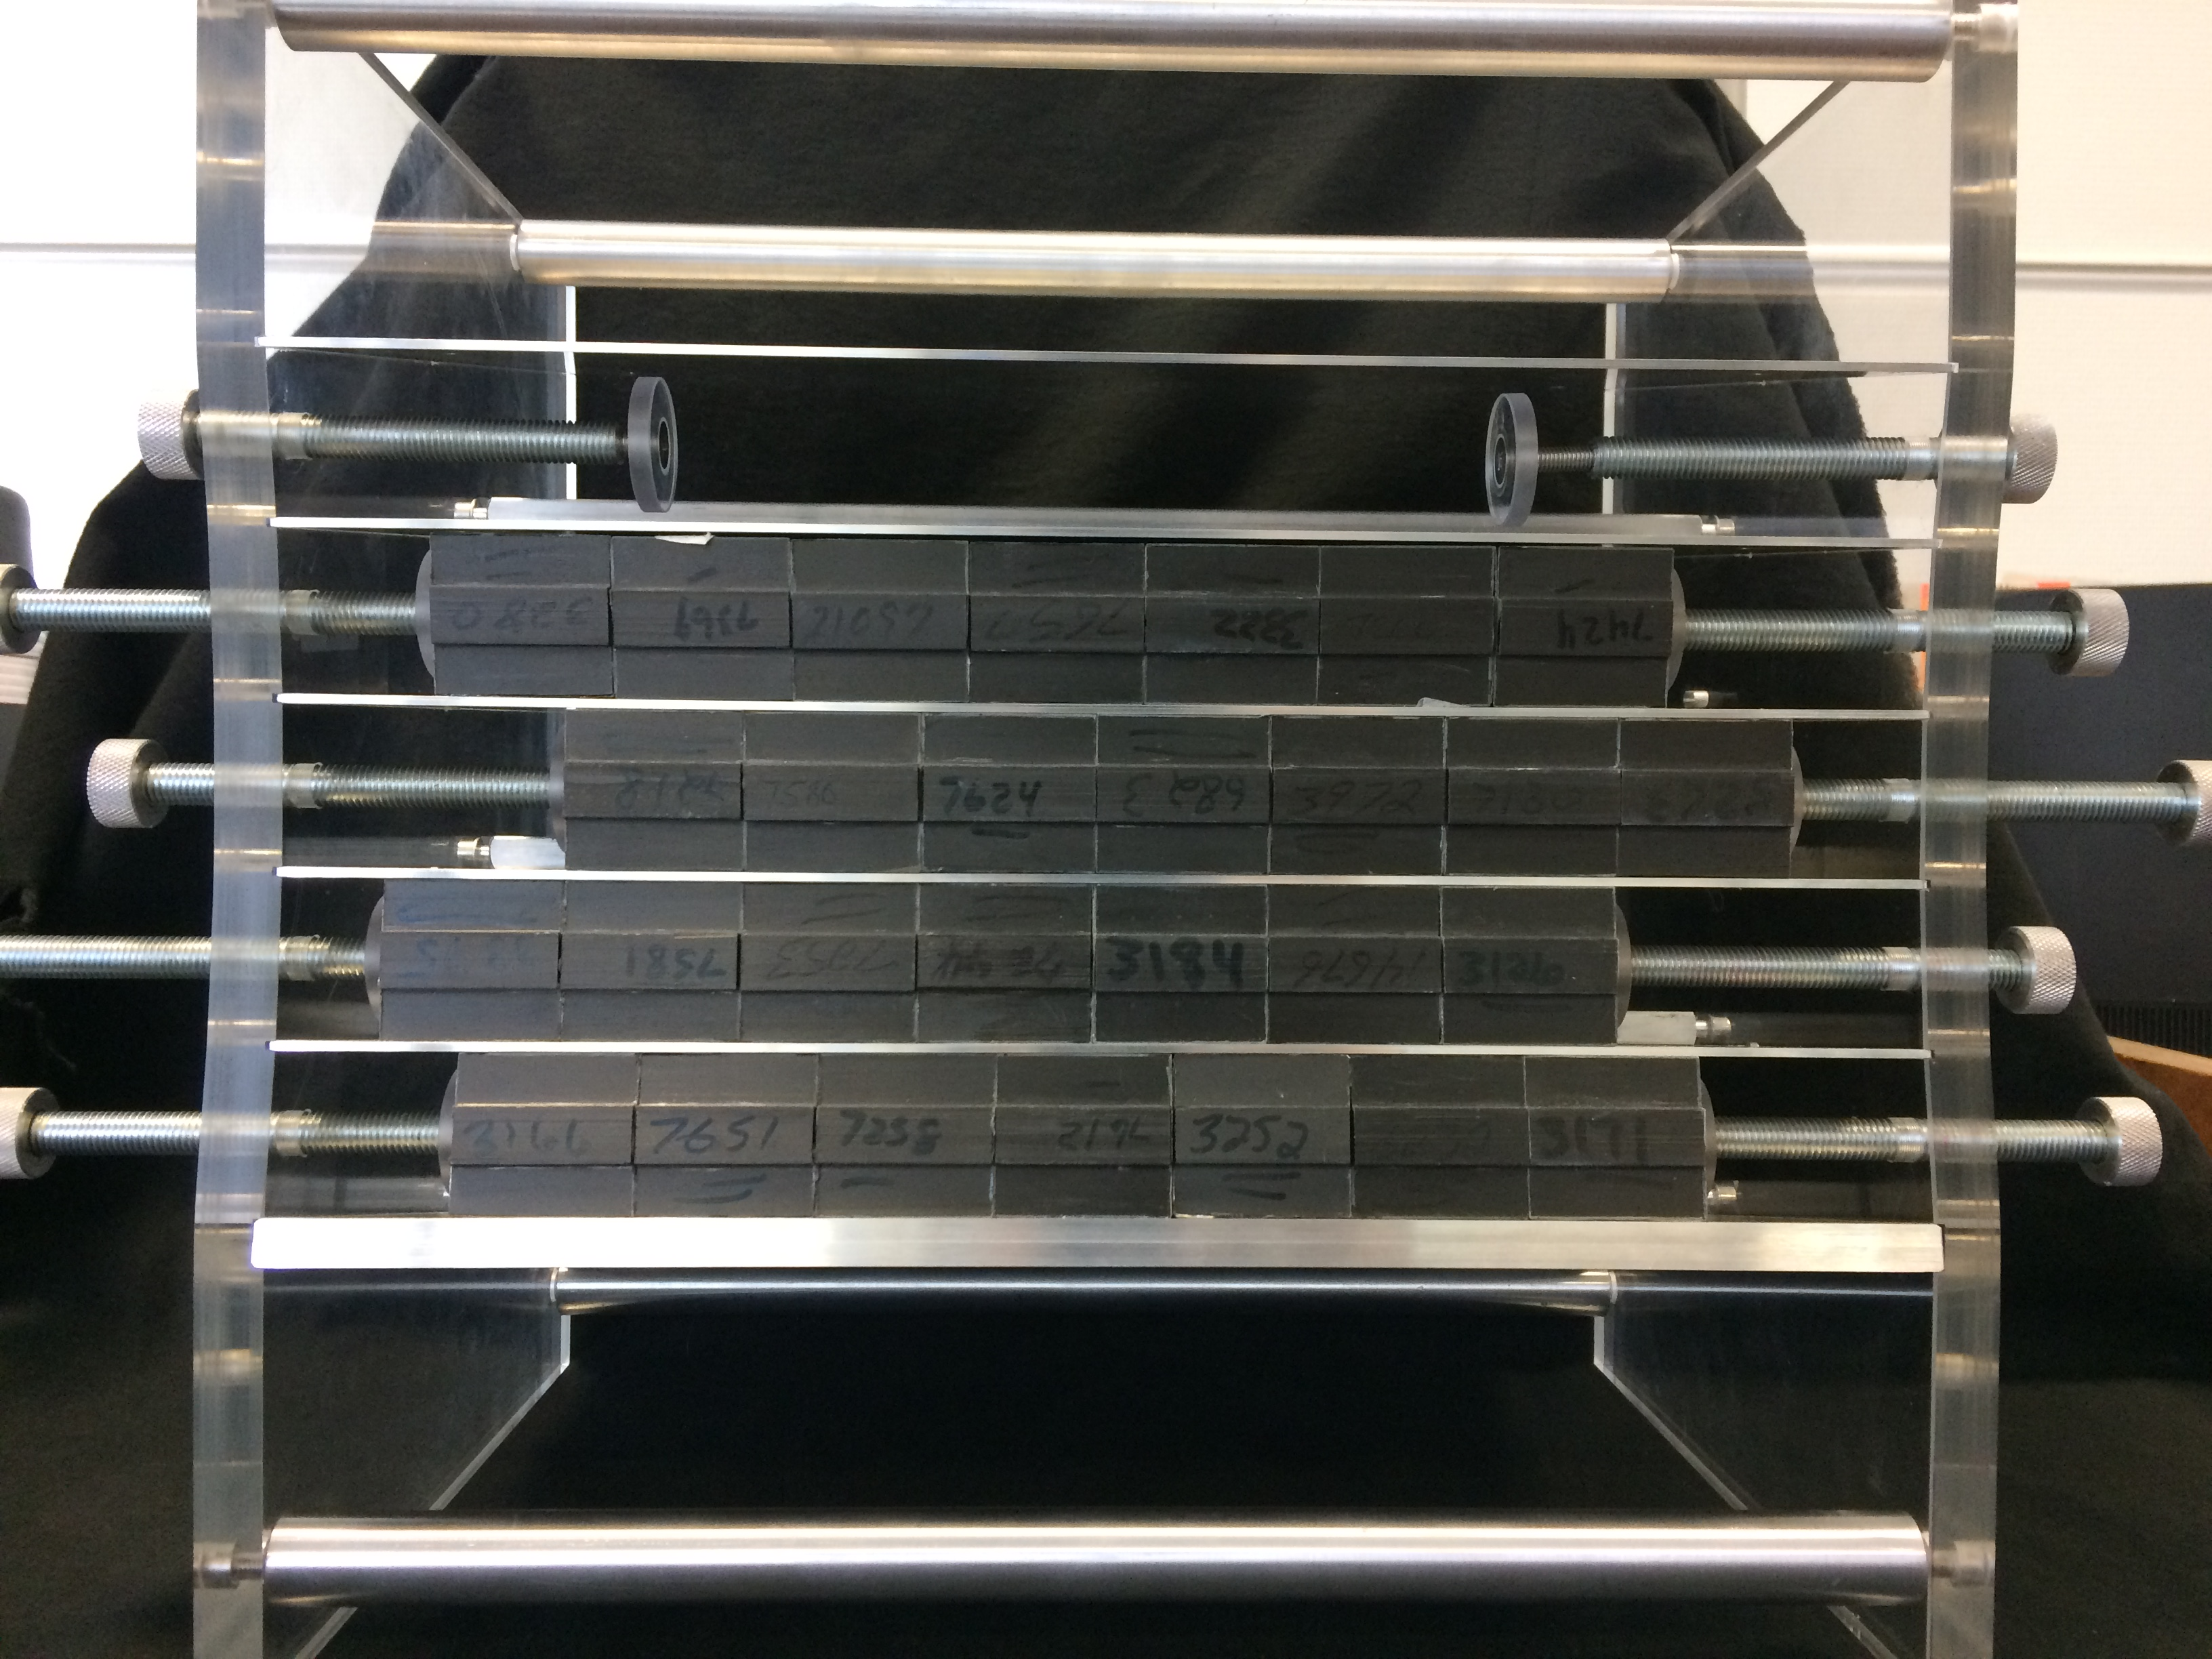
\includegraphics[width=1\textwidth, height=16em]{03_GraphicFiles/chapter3_CLaRySproto/Absorber/images/absorber_picture.JPG}
\caption{Picture of the absorber detector in its mechanical support.}
\label{chap3::fig::absorberPicture}
\end{subfigure}
\begin{subfigure}[b]{.5\textwidth}
\centering
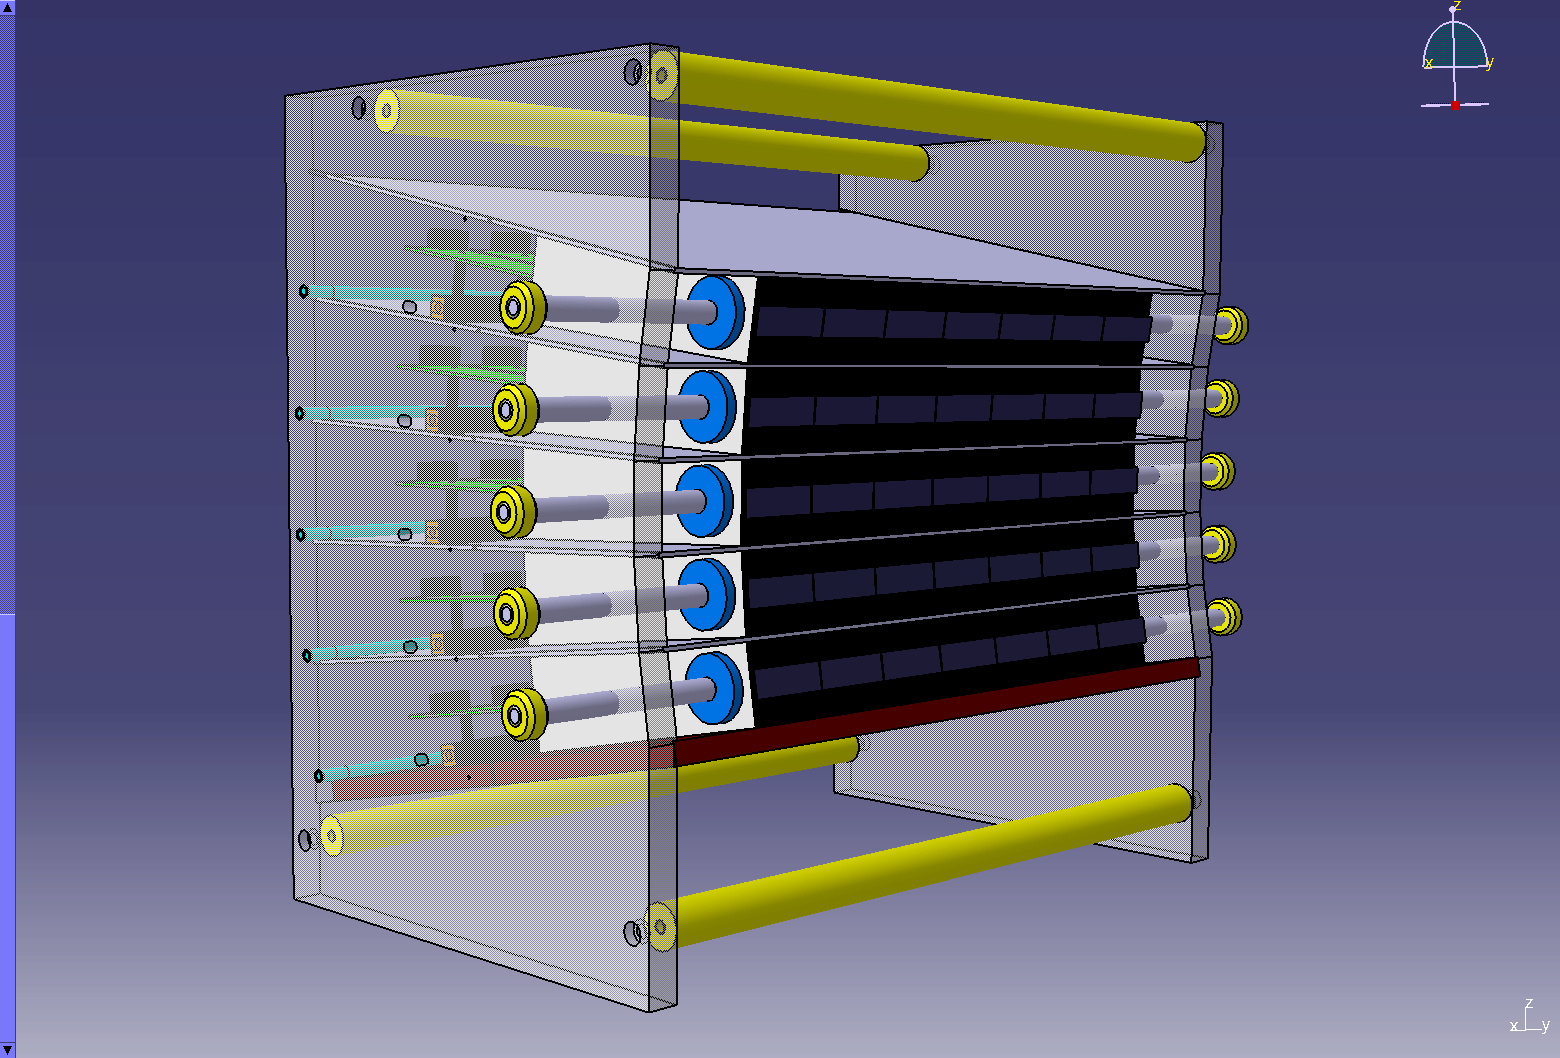
\includegraphics[width=1\textwidth, height=16em]{03_GraphicFiles/chapter3_CLaRySproto/Absorber/images/Absorbeur.jpg}
\caption{Scheme of the absorber detector with its mechanical support.}
\label{chap3::fig::absorber30Scheme}
\end{subfigure}
\caption{Absorber front view with the \gls{bgo} block lines arranged in the mechanical support (a). Scheme of the \gls{bgo} absorber with its mechanical support (b).}
\label{chap3::fig::absorber_scheme}
\end{figure}

%%%%%%%%%%%%%%%%%%%%%%%%%%%%%%%%%%   HODOSCOPE  %%%%%%%%%%%%%%%%%%%%%%%%%%%%%%%%%%%%%%%%%%%%

\subsection{Beam tagging hodoscope}\label{chap3::subsec::hodoscope}

A beam tagging hodoscope is being developed in parallel to the two gamma cameras, mainly for background rejection and reconstruction optimization purposes [CIT]. As already mentioned, the detection of prompt-gammas (with mechanical or \enquote{electronical} collimation), is affected by the presence of other secondary particles produced during the ion beam irradiation, mainly neutrons. This background source can be efficiently identified and removed my applying \gls{tof} selection windows to the data acquisition. The \gls{tof} measurements can be performed using the accelerator radio-frequency signal as reference, but a direct beam detection results to be more accurate. An auxiliary detector is then needed before the beam interaction in the patient.\\ 
The \gls{clarys} hodoscope prototype is designed to provide space and time information about the incoming primary beam, particle by particle or bunch by bunch, depending on the beam intensity and detector efficiency and rate acceptance which must be characterized. In addition to the already explained use of the time information, a space primary particle tagging can be used to improve the reconstruction accuracy and constraint the possible reconstructed emission vertex in case of analytic reconstruction approach for both the multi-collimated and Compton cameras (see chapter~\ref{chap::2}).\\  
The detector under development is based on squared 1~mm$^{2}$ polystyrene scintillating fibers BCF-12, 140~mm in length, provided by Saint Gobain~\parencite{SaintGobain2017}. A picture of the hodoscope on its mechanical support (detailed in the following) is presented in \figurename~\ref{chap3::fig::HodoscopeMain}. The fibers are arranged into two perpendicular planes for a two-dimensional spatial information: each plane is composed of 128 fibers, for a total active area (for 2D measurements in coincidence) of 128$\times$128~mm$^{2}$. The active detector surface is completely covered with black reflective tape, which shields from external light. The scintillation light produced in the fibers by a ionizing particle deposing energy is transported to the read-out system via FORETEC optical fibers (1.55~cm diameter, 1~m length), which are connected to the scintillating fibers thanks to a custom mechanical support and to a proper gluing process (see \figurename~\ref{chap3::fig::HodoMounting}). Each scintillating fibers is read-out on both sides to optimize the detector efficiency and improve the time resolution which is not depending on the interaction position along the fiber with this configuration, so that the total number of read-out channels is 512. The signal read-out is ensured by 8 multi-anode \glspl{pm} Hamamatsu H8500~\parencite{Hamamatsu2006} shown in \figurename~\ref{chap3::fig::PMH8500}. The optical fibers are connected to the \gls{pm} anode surfaces through a plastic custom mask, shown in \figurename~\ref{chap3::fig::PMmask}. The \glspl{pm} are equipped with custom black boxes which operate as mechanical support and external light protection (see \figurename~\ref{chap3::fig::HodoMounting}). In order to provide further light isolation, the whole \gls{pm} boxes are covered with black tape.\\
The optical fibers are connected to the \glspl{pm} with the aim of increasing the maximum counting rate. 4 \glspl{pm} are dedicated to the read-out of the horizontal fibers, and 4 to the vertical ones, and the neighboring fibers are connected to different \glspl{pm}. An active area of 4$\times$4~mm$^{2}$ on the two planes is then read-out by all the 8 \glspl{pm}. Moreover, the two sides of the same scintillating fiber are connected on the same \gls{pm}. This fiber connection logic also improve the detector robustness; in case of problem on one \gls{pm}, only 1~mm each 4~mm is lost on a single plane, so that the detection of the beam is still possible on the whole active area.\\  
Each \gls{pm} is connected to a single custom \gls{fe} card. The hodoscope \gls{fe} cards have been developed by the \gls{ipnl} electronics group: their design is described in section~\ref{chap3::subsubsec::HodoFEcard}. 8 \gls{fe} cards are then used for the read-out, and the collected data are sent to the acquisition system described in section~\ref{chap3::subsec::cameraElectronicsDAQ}.

\begin{figure}[!htbp]
\centering
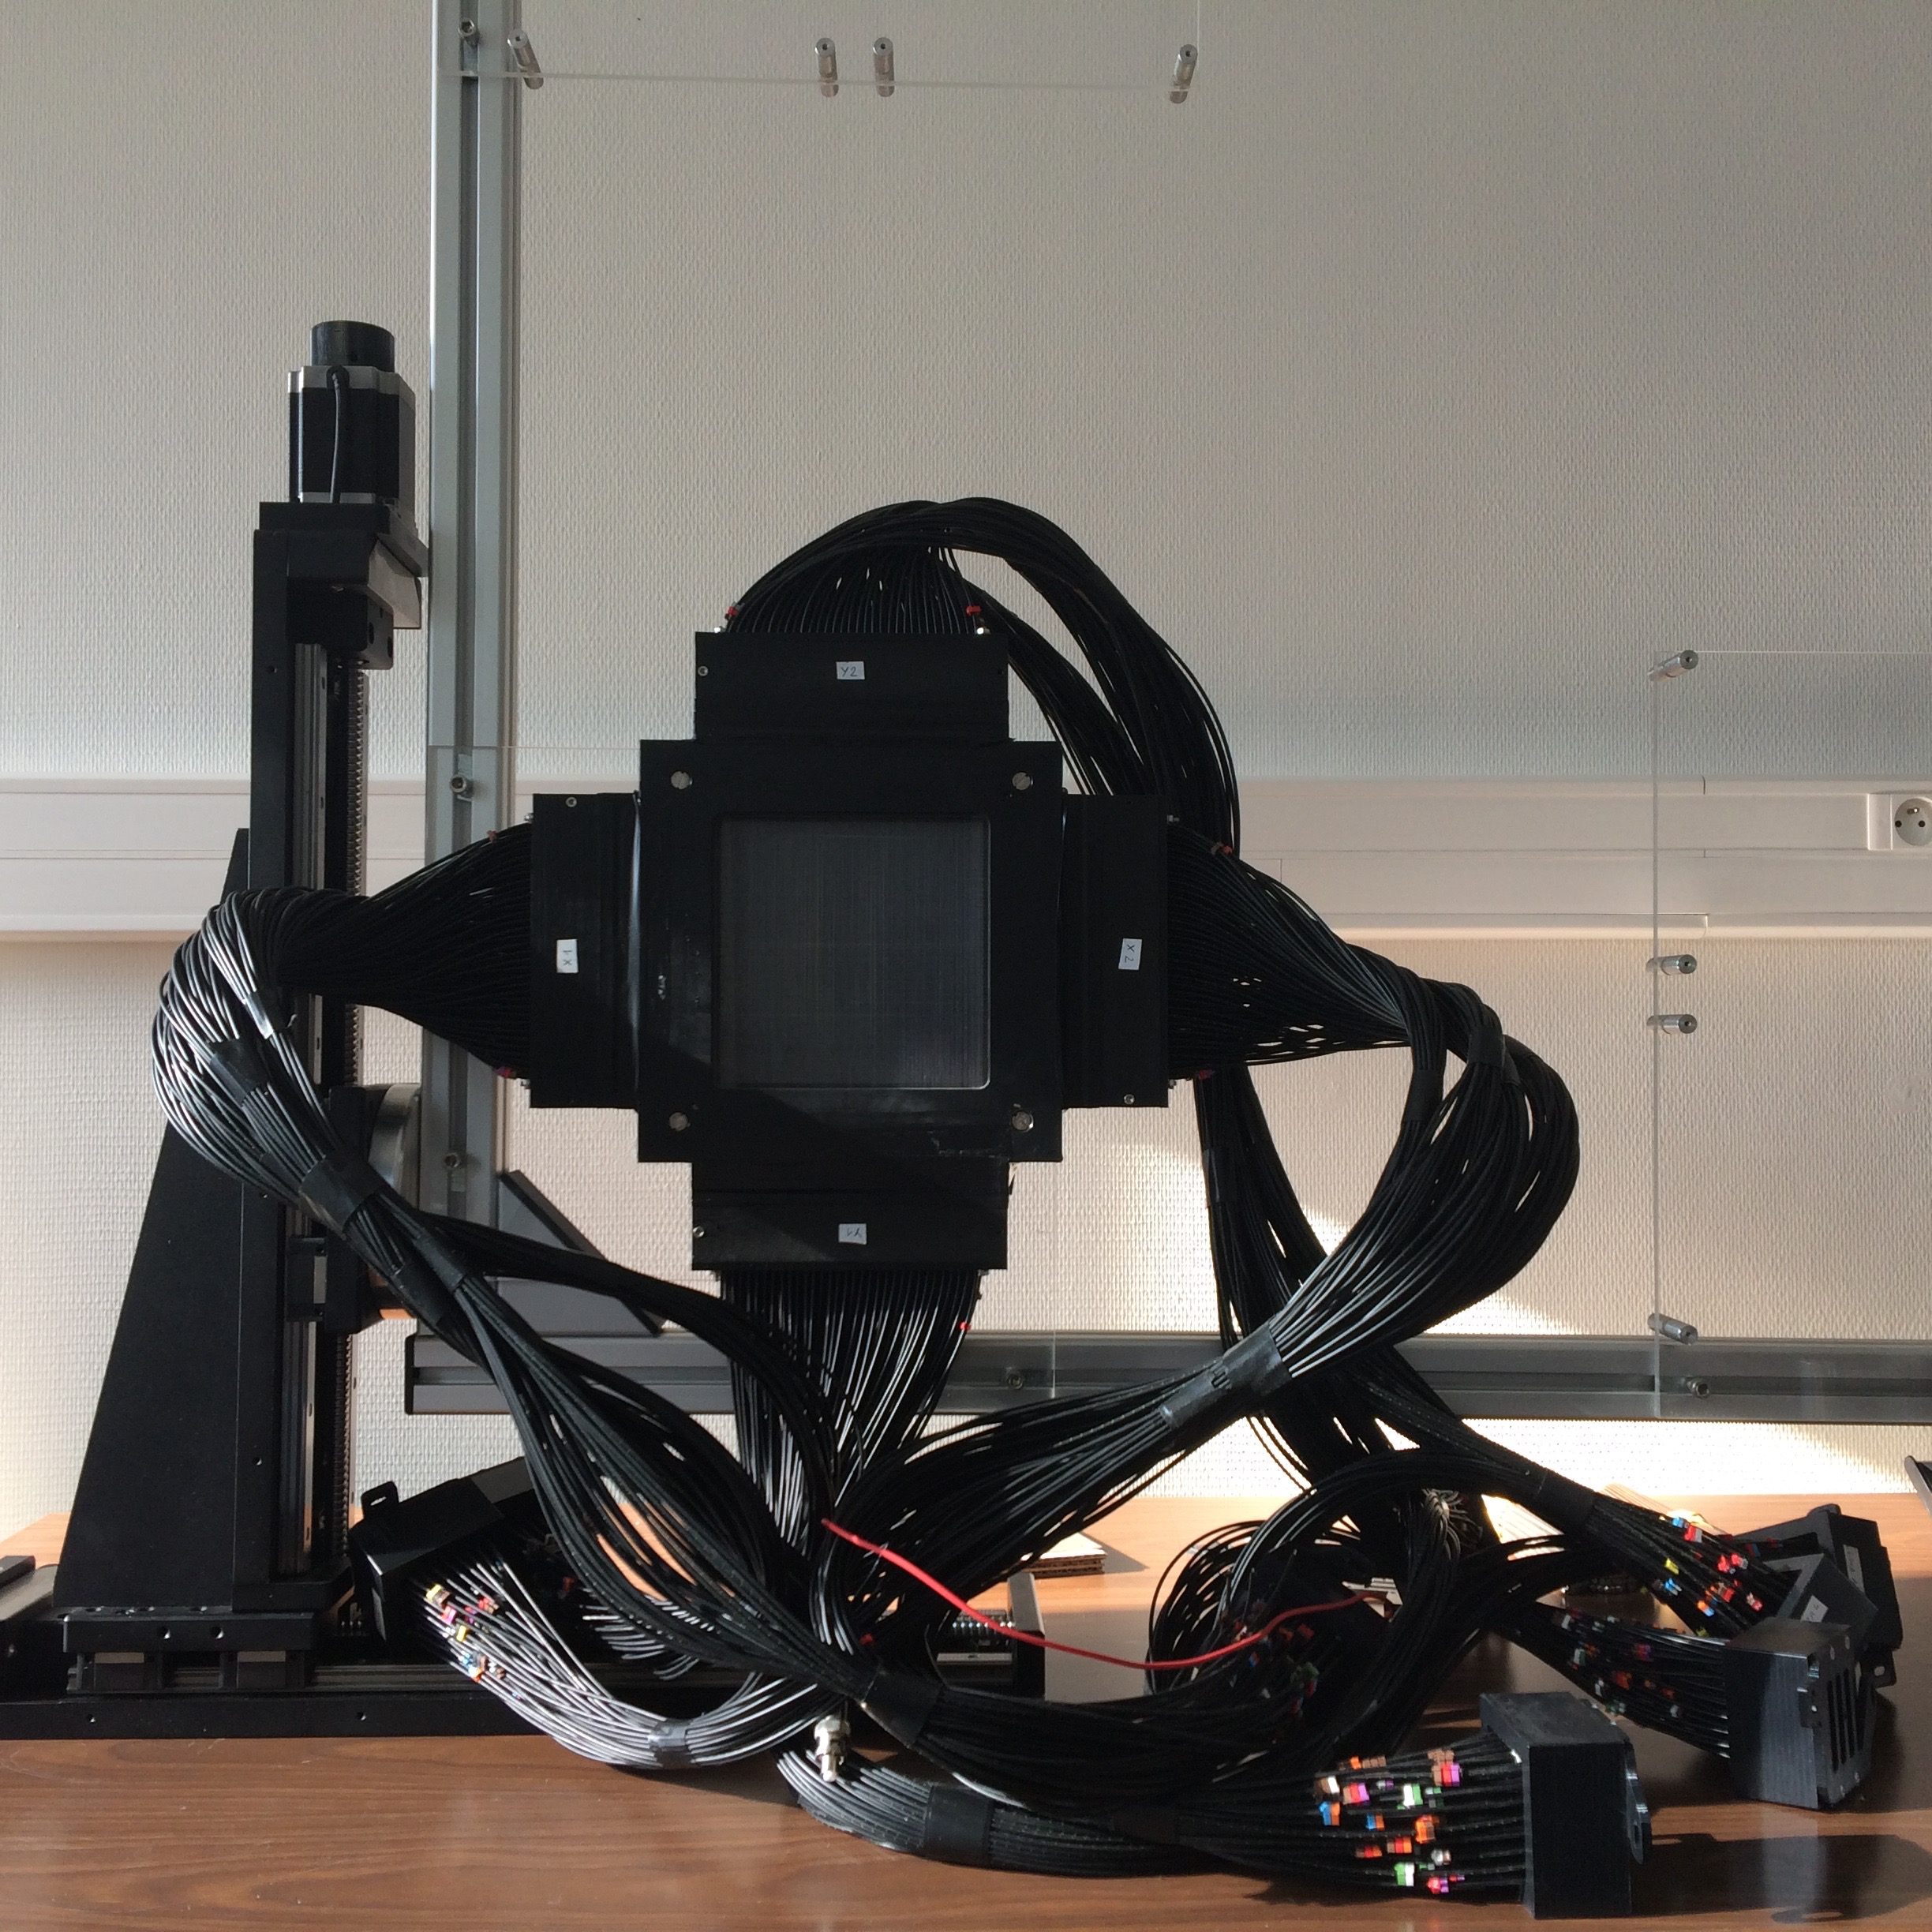
\includegraphics[width=0.6\textwidth]{03_GraphicFiles/chapter3_CLaRySproto/Hodoscope/Hodoscope_onTable.jpg}
\caption{128$\times$128 scintillating fiber hodoscope on its 2-dimensional moving support.}
\label{chap3::fig::HodoscopeMain}
\end{figure}

\begin{figure}
\begin{subfigure}[t]{0.5\textwidth}
\centering
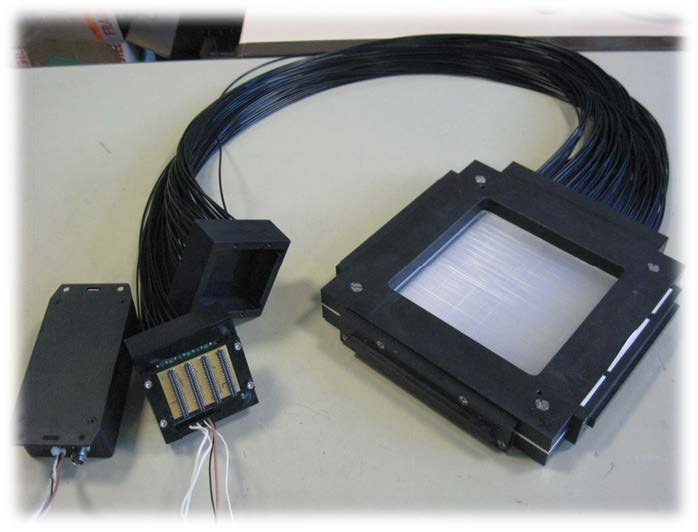
\includegraphics[width=1\textwidth]{03_GraphicFiles/chapter3_CLaRySproto/Hodoscope/Hodoscope_mounting.jpg}
\caption{Scintillating fiber hodoscope during mounting process.}
\label{chap3::fig::HodoMounting}
\end{subfigure}
\begin{subfigure}[t]{0.5\textwidth}
\centering
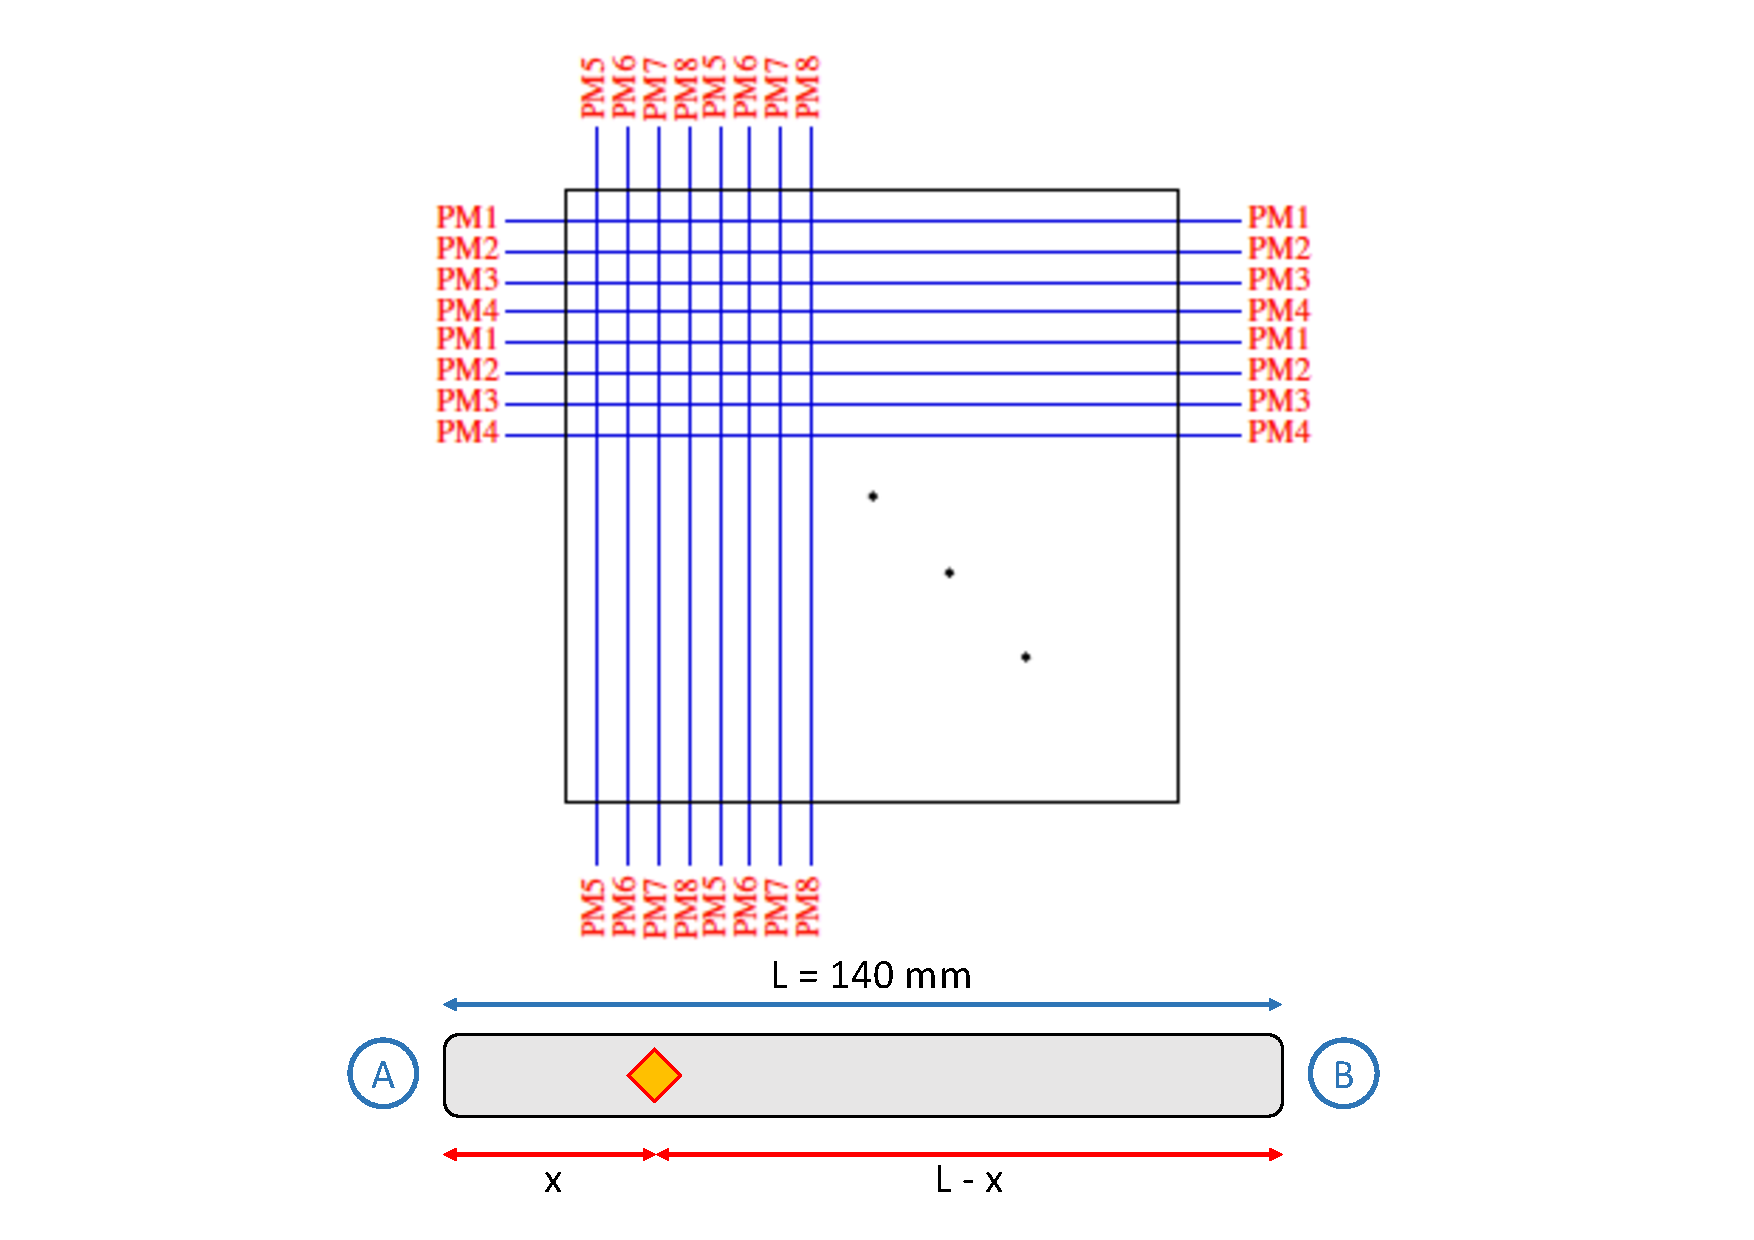
\includegraphics[width=1\textwidth]{03_GraphicFiles/chapter3_CLaRySproto/Hodoscope/hodoPMfiberConnection.pdf}
\caption{Scheme of the scintillating fiber connection to the \glspl{pm} (top) and of the double-sided fiber read-out (bottom).}
\label{chap3::fig::HodoPMfiberConn}
\end{subfigure}
\newline
\begin{subfigure}[t]{0.5\textwidth}
\centering
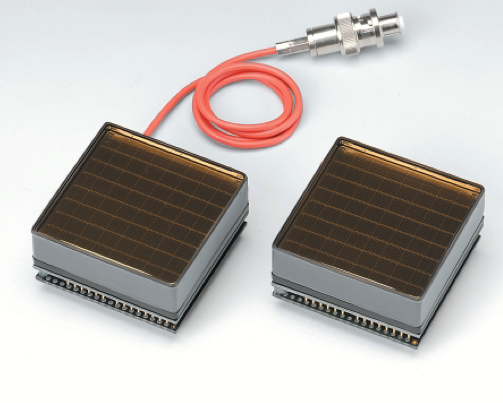
\includegraphics[width=1\textwidth, height = 6cm]{03_GraphicFiles/chapter3_CLaRySproto/Hodoscope/H8500.png}
\caption{Hodoscope read-out \glspl{pm} Hamamatsu H8500.}
\label{chap3::fig::PMH8500}
\end{subfigure}
\begin{subfigure}[t]{.5\textwidth}
\centering
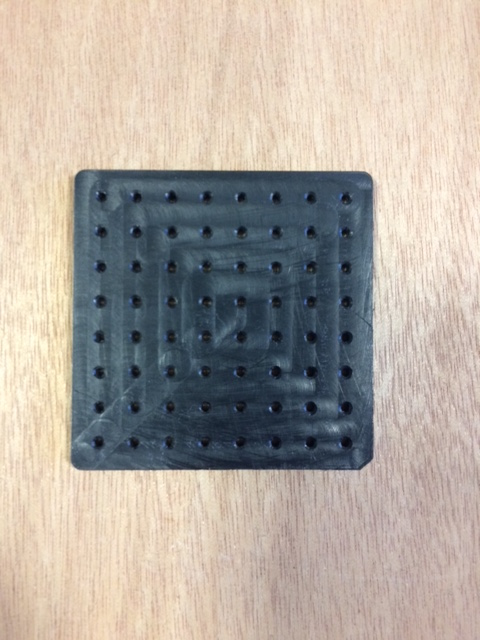
\includegraphics[width=1\textwidth, trim = {0 3cm 0 5cm}, clip = true, height = 6cm]{03_GraphicFiles/chapter3_CLaRySproto/Hodoscope/Hodoscope_PMmask.JPG}
\caption{\gls{pm} plastic mask for optical fiber connection.}
\label{chap3::fig::PMmask}
\end{subfigure}
\caption{Details of the scintillating fiber hodoscope setup.}
\label{chap3::fig::HodoscopeParts}
\end{figure}


\subsubsection{Hodoscope Front-End card}\label{chap3::subsubsec::HodoFEcard}

The hodoscope is designed to tag in space and time the incoming beam ions, so that the signal read-out must be optimized to provide accurate time measurements and an high detection rate acceptance, with reduced dead time and detection efficiency close to 100\%. In particular, the design requirements include a maximum counting rate acceptance of 10$^{8}$~Hz per detection plane, with a time resolution of 1~ns~\parencite{Krimmer2014}.  The hodoscope \gls{fe} card shown in \figurename~\ref{chap3::fig::HodoscopeFEcard} has been developed by the \gls{ipnl} electronics group to fulfill the listed requirements. The Hamamatsu \gls{pm} is connected to the 64-channel connector (4 connectors of 16 channels each) and two custom \glspl{asic} are dedicated to the data first treatment (32 channels each).\\
  
\begin{figure}
\centering
\begin{subfigure}[t]{.34\textwidth}
\centering
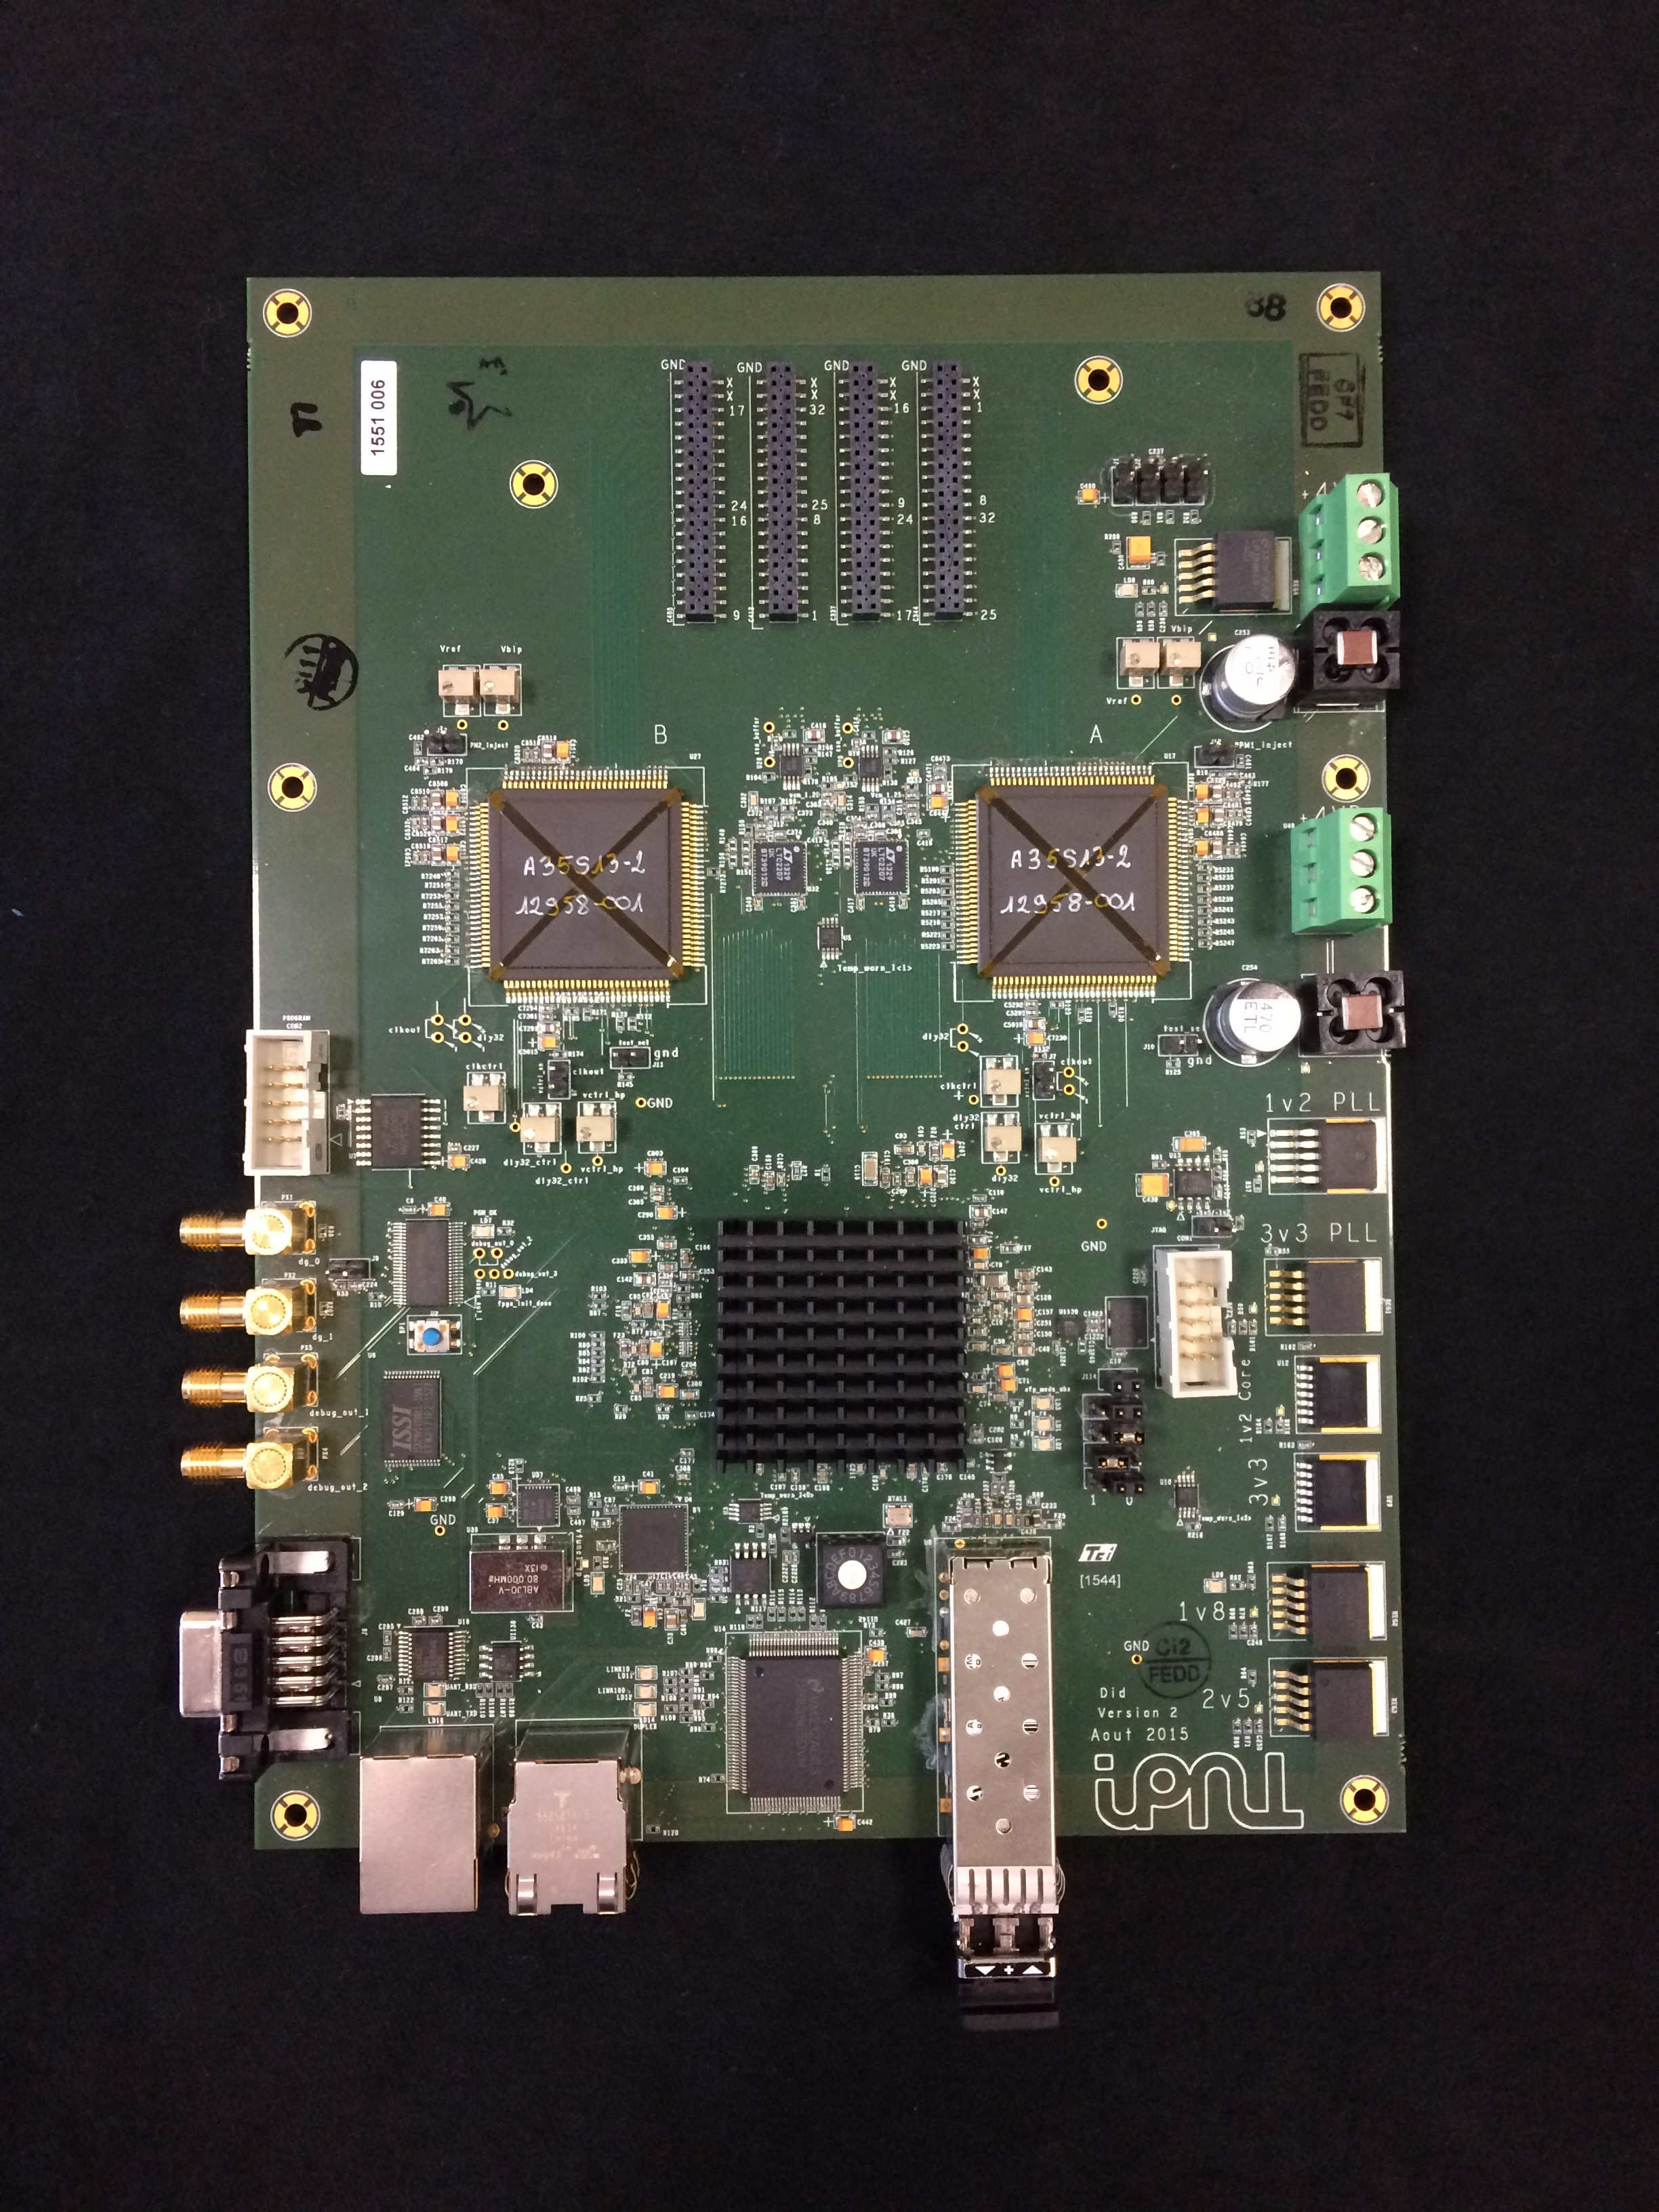
\includegraphics[width=\linewidth, height = 6cm]{03_GraphicFiles/chapter3_CLaRySproto/Hodoscope/HodoCard1.jpg}
\caption{Hodoscope \gls{fe} card.}
\label{chap3::fig::HodoscopeFEcard}
\end{subfigure}
\begin{subfigure}[t]{.56\textwidth}
\centering
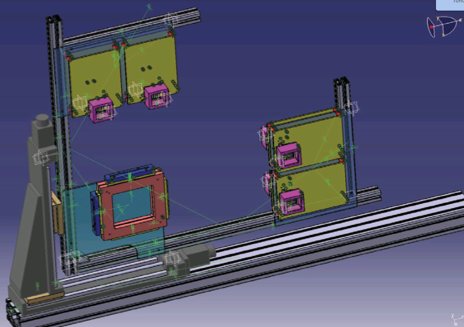
\includegraphics[width=\linewidth, trim = {0 0 1cm 0}, clip = true, height = 6cm]{03_GraphicFiles/chapter3_CLaRySproto/Hodoscope/HodoScheme.png}
\caption{Hodoscope mechanical support scheme.}
\label{chap3::fig::HodoscopeSchemeMech}
\end{subfigure}
\caption{HODOPIC board (a) and scheme of the beam-tagging hodoscope two-dimensional moving support (b).}
\label{chap3::fig::HodoPic}
\end{figure}

A first version of the \gls{fe} \gls{asic} has been developed in 2012 by the group \gls{micrhau} for the read-out of 8 channels (designed for the 32$\times$32 fiber hodoscope prototype described in section~\ref{chap3::subsubsec::SmallHodoProto}). The input part is composed of a current conveyor, and the output one has two sections: a current discriminator and a charge pre-amplifier for the charge measurements in test mode~\parencite{Deng2012, Deng2013}. In addition, the \gls{asic} gain can be tuned channel by channel, so that the response of each \gls{pm} output channel can be fine tuned with respect to the others.\\
The second version of the \gls{asic} includes all the features of the first version, with the addition of a \gls{tdc} based on a 160~MHz clock for a more accurate time tagging of the detected events. Moreover, a \gls{dll} is installed to divide the main clock in 32 intervals: for each event, the \gls{dll} state is stored in a 32 bit register and then encoded in a 5-bit Gray decoder. As a result, the \gls{tdc} has a 6.25~ns dynamics, with a sampling step of 195~ps and a time resolution of 58.8~ps \gls{rms}, for a maximum accepted rate of 10$^{8}$~Hz~\parencite{Deng2012b}.\\
The third and final \gls{asic} version, called HODOPIC, is adapted to the big size hodoscope (512 read-out channels), with the extension to 32 channels and with the \gls{tdc} implemented on the second version. An external \gls{adc} is used for the charge measurement in test mode for a single channel, selected via slow control. All the \gls{asic} outputs are sent to a \gls{fpga} installed on the card for the actual time measurement and data decoding. The \gls{fpga} finally handles the data transmission to the acquisition system, depending on the card version.\\
A first card has been developed to test the first \gls{asic} version with the 32$\times$32 fiber hodoscope. It is based on a \gls{fpga} Altera Cyclone III~\parencite{Altera2012} and on 9 \glspl{asic}, with a LabVIEW acquisition. A single card is enough for the read-out of the complete small hodoscope prototype. This first setup has been tested on beam at the \gls{ganil} and the \gls{hit}, and a sub-ns time resolution has been verified, together with the expected 1~mm spatial resolution on the two fiber planes and an efficiency of more then 90\% at a 10$^{6}$ acquisition rate.\\
The second prototype of the card, shown in \figurename~\ref{chap3::fig::HodoscopeFEcard}, has been adapted to the 512-channel hodoscope described in the previous section and to the gamma camera acquisition system described in~\ref{chap3::subsec::cameraElectronicsDAQ}: each card has two HODOPIC \glspl{asic}, 32 channels each, so that it is designed for the read-out of a single 64-anode \gls{pm}. 8 cards are then needed for the read-out of the whole hodoscope. This version is based on a \gls{fpga} Altera StratixII GX~\parencite{Altera2009}, and the connection to the acquisition is ensured by a 3~Gbit/s optical link. 4 digital input-output channels are installed for test and validation purpose, together with an Ethernet port.\\
Further details about the different card versions and the applied validation tests can be found in~\cite{Chen2017}.\\
The hodoscope card firmware has been developed in 2017 and tested in simplified versions on beam, as detailed in chapter~\ref{chap::6}.
           

\subsubsection{Hodoscope mechanical support}\label{chap3::subsubsec::HodoMechanics}

The beam tagging hodoscope is set between the beam nozzle and the patient and requires a dedicated mechanical support. In order to profit of the large active area and to be able to remotely control the hodoscope position in the beam transverse plane, the detector is mounted on a 2-dimensional moving table (see the picture in \figurename~\ref{chap3::fig::HodoscopeMain}), which also supports the \gls{fe} cards. Detector and \gls{fe} cards are then integral and translate together. A scheme of the moving table is given in \figurename~\ref{chap3::fig::HodoscopeSchemeMech}.\\
The 2-axis table is provided by Beijing Winner Optical Instruments; it is composed of two motorized linear stages, connected via a right angle bracket. The two stages have a moving range of 30~cm each and the stepper motors have a step resolution of 20~\charmum. The employed motor controller is a Newport XPS-Q8~\parencite{Newport2017}, equipped with 8 channels for the simultaneous control of a maximum of 8 motors. The movements are steered with an online interface or with a LabVIEW based program, which will be integrated in the final setup of the slow control software under development with the cameras.

\subsubsection{Small hodoscope prototypes}\label{chap3::subsubsec::SmallHodoProto}
Before the production of the large active surface hodoscope prototype described in section~\ref{chap3::subsec::hodoscope}, two smaller prototypes have been produced and tested in order to assess the potential of such a kind of detector for the required application. The first and simplest version consisted of one single scintillating fiber per plane, and the readout was performed with two \gls{pm} tubes directly coupled to the scintillating fibers, without optical fibers. A picture of this prototype is given in \figurename~\ref{chap3::fig::singleFibHodo}. This simple version of the detector has been used as a demonstrator of the basic detection principle.\\ 

\begin{figure}
\begin{subfigure}[t]{.5\textwidth}
\centering
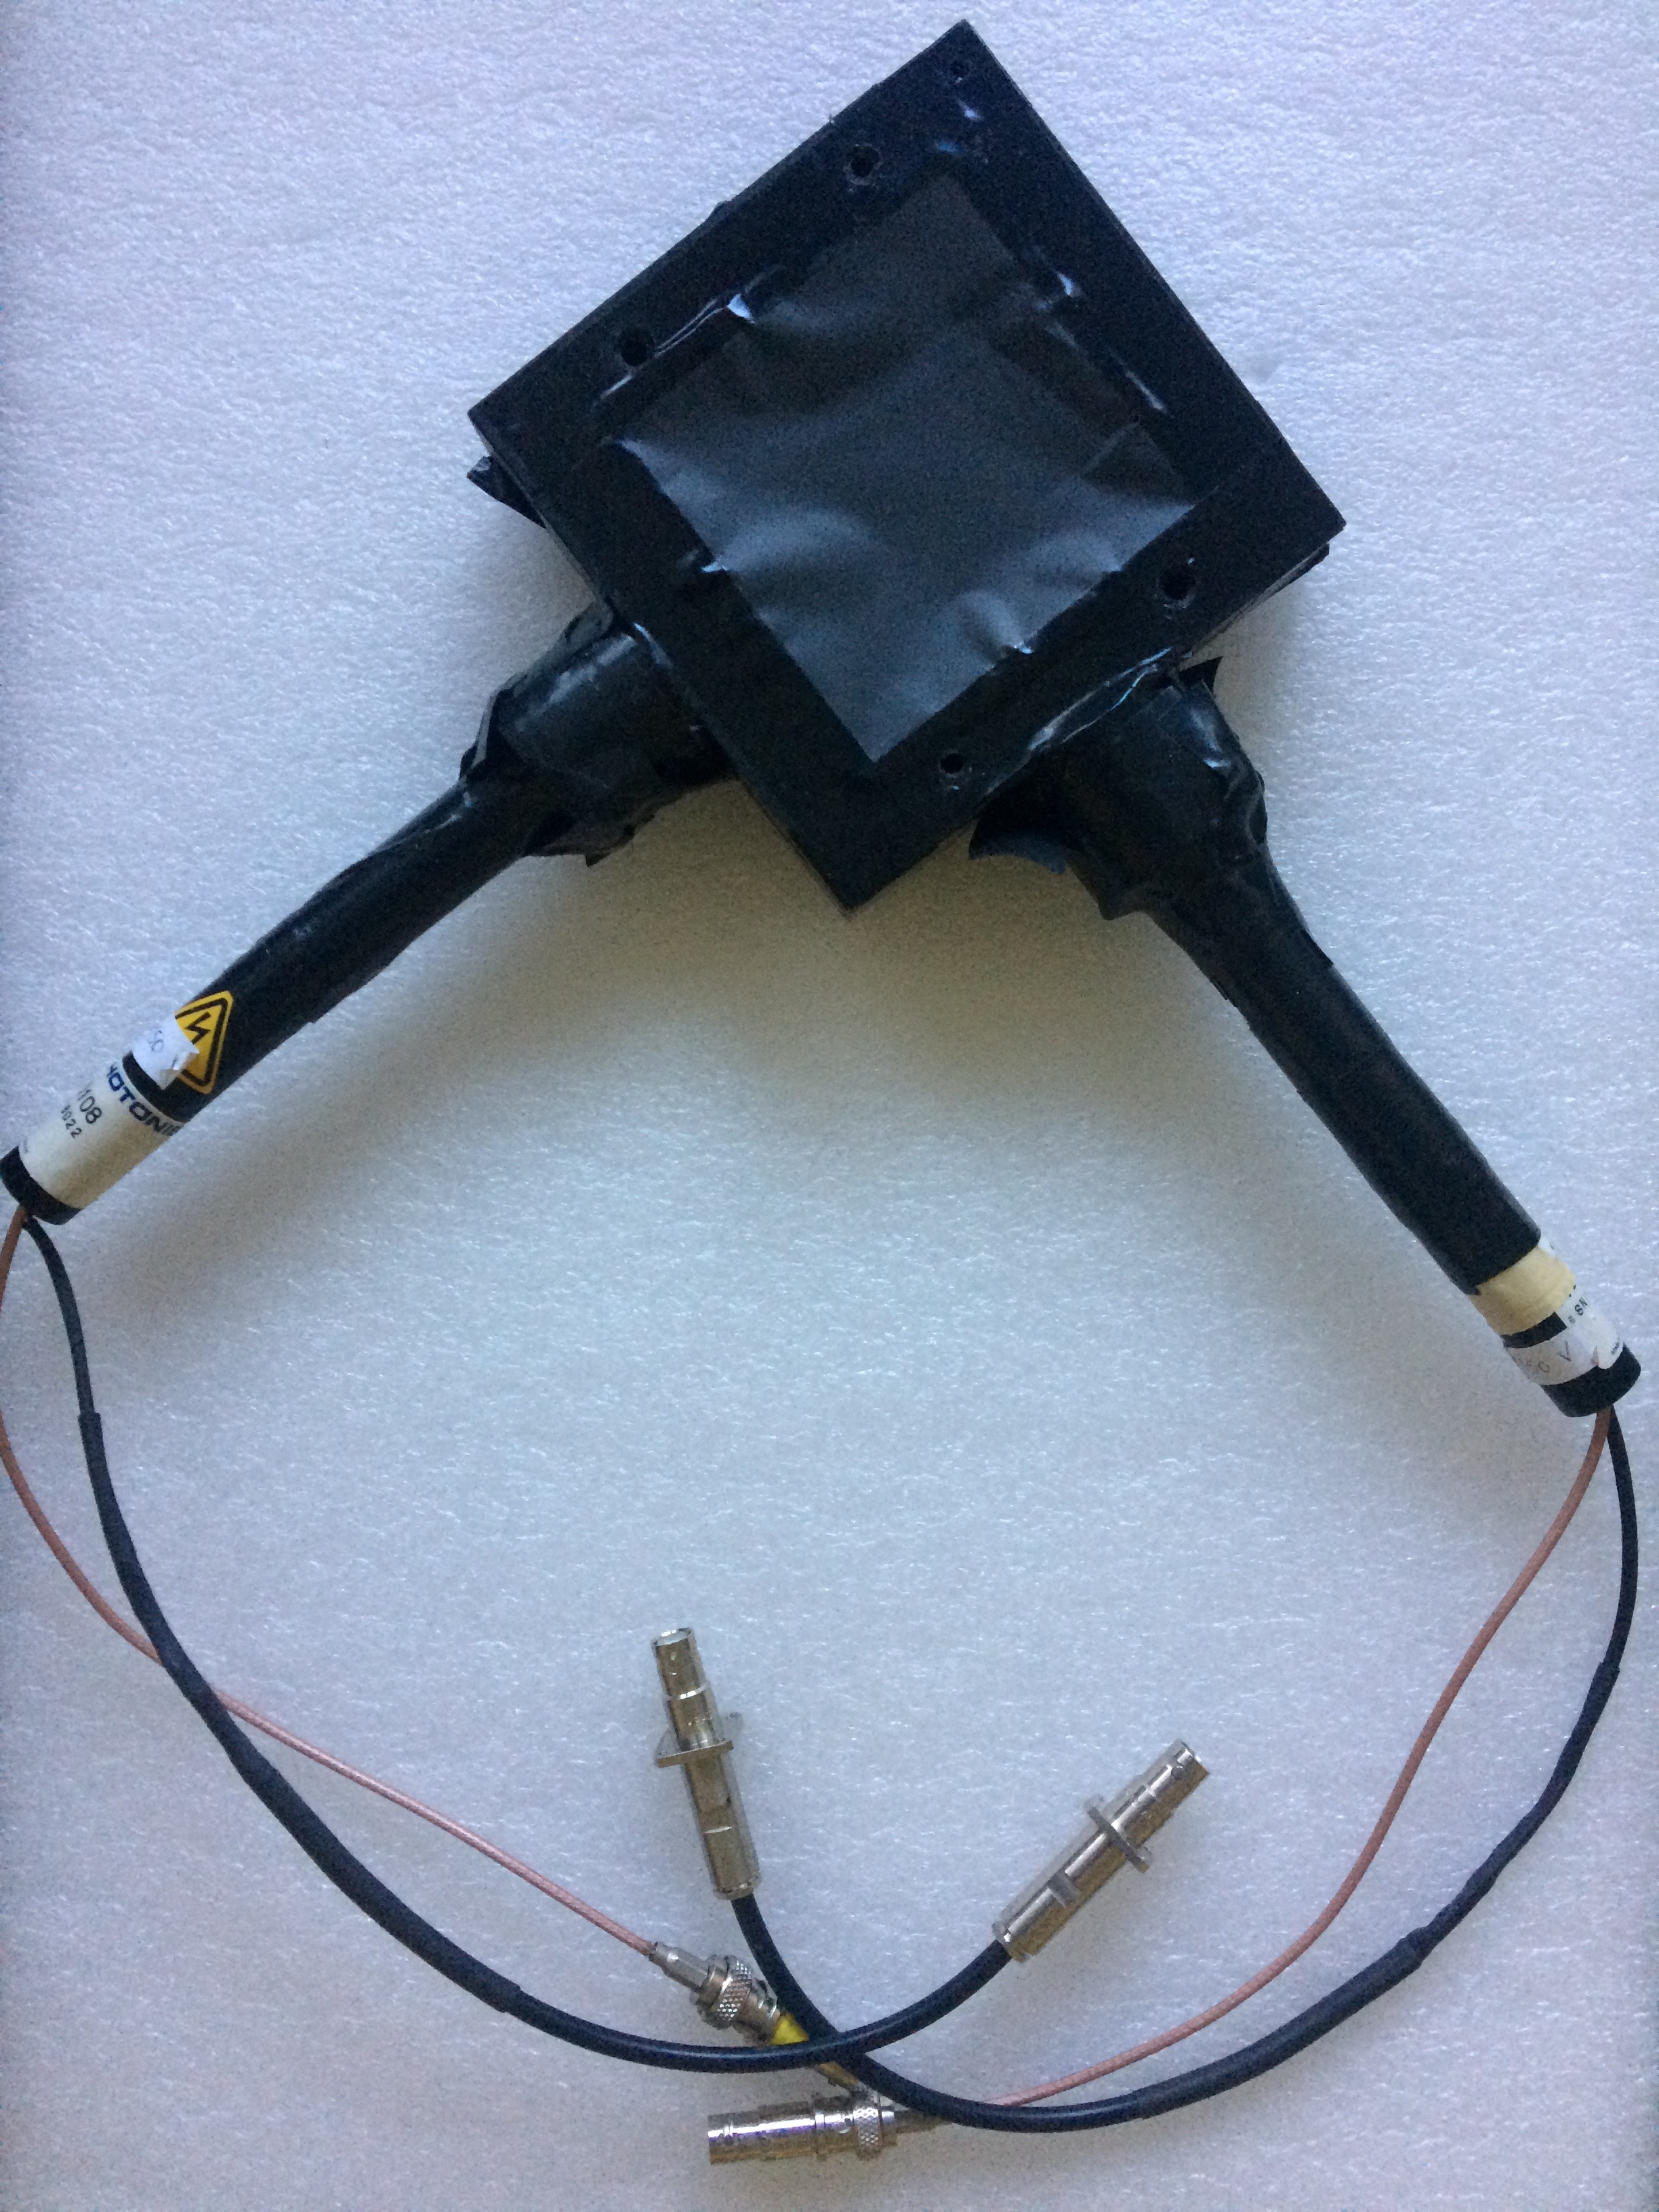
\includegraphics[width=0.8\textwidth]{03_GraphicFiles/chapter3_CLaRySproto/Hodoscope/hodo2.jpg}
\caption{Hodoscope small prototype, 1$\times$1 scintillating fibers.}
\label{chap3::fig::singleFibHodo}
\end{subfigure}
\begin{subfigure}[t]{.5\textwidth}
\centering
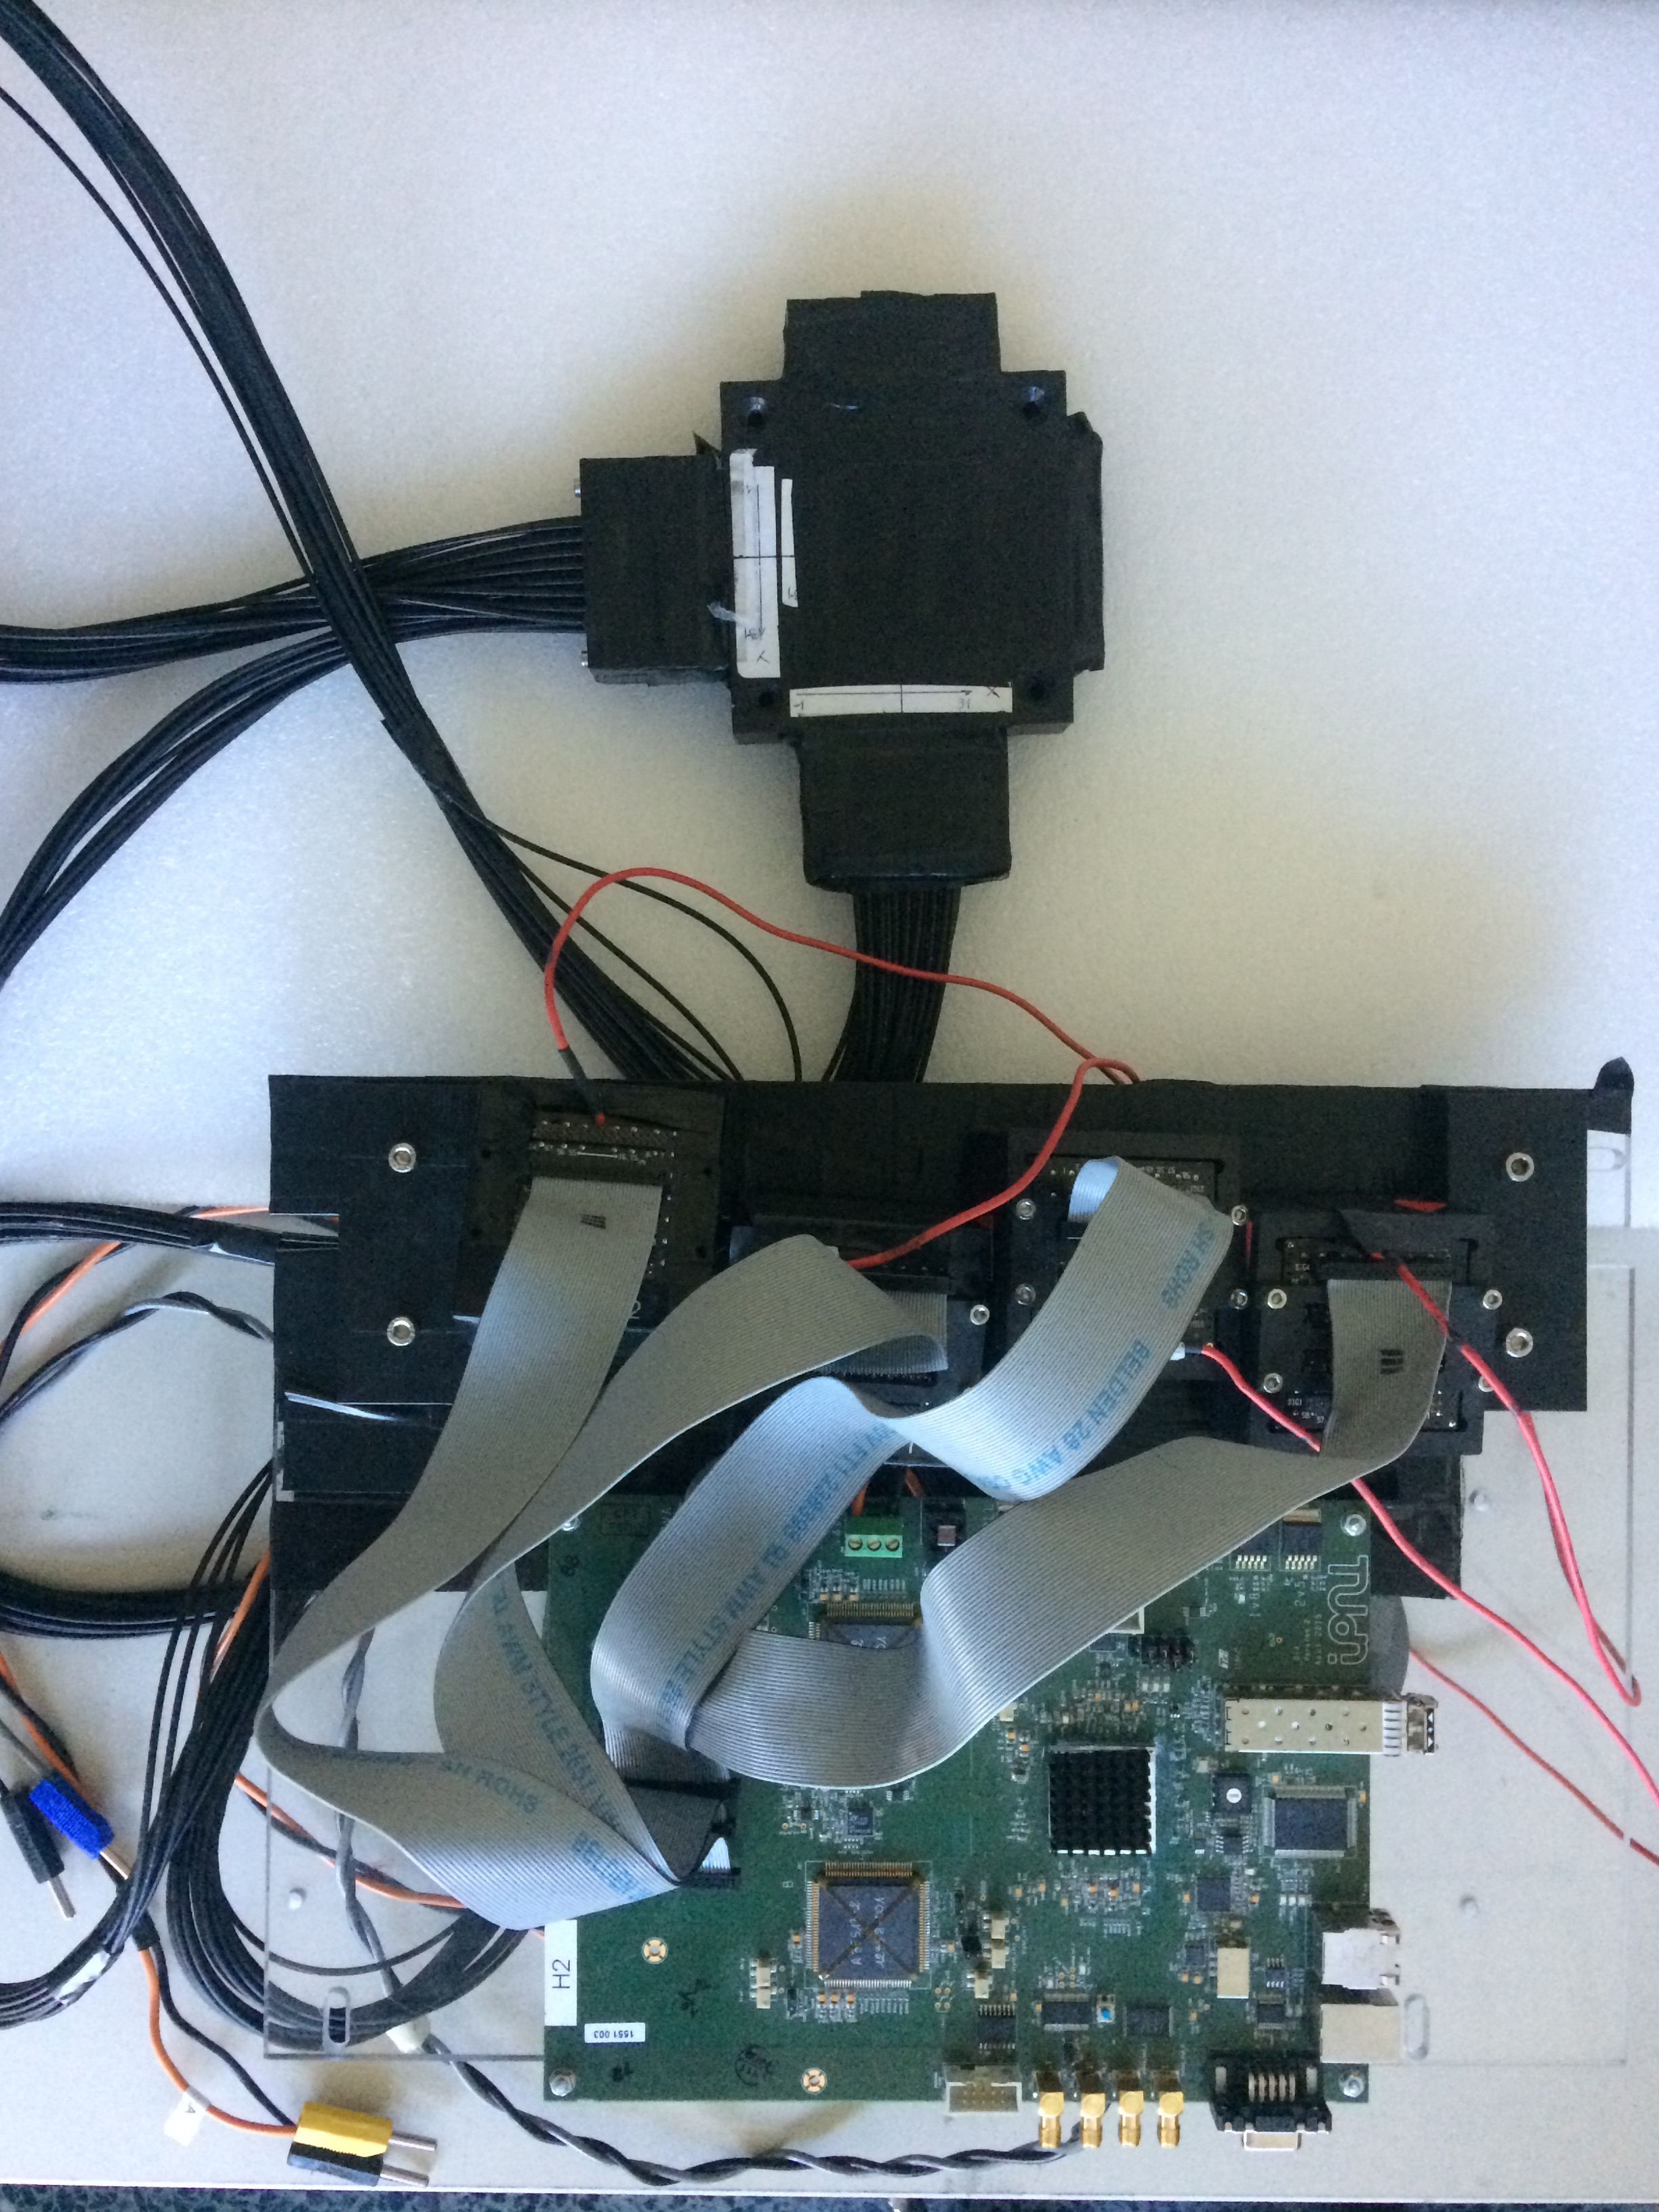
\includegraphics[width=0.8\textwidth]{03_GraphicFiles/chapter3_CLaRySproto/Hodoscope/hodo32_withCard.jpg}
\caption{Hodoscope small prototype, 32$\times$32 scintillating fibers, connected to the HODOPIC \gls{fe} board.}
\label{chap3::fig::Hodoscope32}
\end{subfigure}
\caption{Hodoscope small prototypes.}
\label{chap3::fig::HodoSmall}
\end{figure}

A second small size version of the final detector has been produced with almost the same features as the large area prototype but with simplified read-out logic. It is equipped with two perpendicular planes of 32 1~mm$^{2}$ scintillating fibers each (Saint Gobain BCF-10~\parencite{SaintGobain2017}), with a length of 4~cm and a total active area for a 2D read-out of 32$\times$32~mm$^{2}$. As in the big hodoscope, the scintillating fibers are coupled to FORETEC optical fibers which transfer the scintillation light to 4 Hamamatsu H8500 \glspl{pm}. 16 channels per \gls{pm} are used, so that 2 \glspl{pm} are dedicated to the horizontal fibers and 2 to the vertical ones, and the signal read-out is performed on a single side of the scintillating fibers. As the total number of read-out channels is 64, a single \gls{fe} card is enough for the whole detector. In \figurename~\ref{chap3::fig::Hodoscope32} the 32$\times$32-fiber hodoscope prototype is shown together with its \gls{fe} card; 4 connections cables (16 channels each) are used to couple the \glspl{pm} to the \gls{fe} card.\\
The 32$\times$32-fiber hodoscope prototype has been tested in 2014 on proton and carbon ion beams (at the \gls{ganil} - 75~MeV/u $^{13}$C, \gls{hit} - protons and carbon ions at various energy, \gls{ipno} - 25~MeV protons) with the first version of the \gls{fe} card (see section~\ref{chap3::subsubsec::HodoFEcard}): an efficiency of more than 90\% has been retrieved, with a time resolution of 1~ns \gls{fwhm} (timing measurements performed with respect to the accelerator high frequency signal). Some more details about this beam tests results are given in chapter~\ref{chap::6}. The final version of the \gls{fe} card has been also tested with this detector, and the test description and results are presented in chapter~\ref{chap::6}.  
   

%%%%%%%%%%%%%%%%%%%%%%%%%%%%%%%%%%   ELECTRONICS/DAQ  %%%%%%%%%%%%%%%%%%%%%%%%%%%%%%%%%%%%%%%%%%%%

\subsection{Camera acquisition system}\label{chap3::subsec::cameraElectronicsDAQ}

The \gls{tof} gamma cameras developed by the \gls{clarys} collaboration are composed of various detection sections: beam tagging hodoscope and \gls{bgo} absorber for the multi-slit collimated camera, with the addition of the silicon scatterer stack for the Compton camera. The acquisition system must be able to handle the data flux from the different components, for a total of 20 \gls{fe} cards (7 for the silicon scatterer, 8 for the hodoscope and 5 for the absorber), select the events according to the chosen trigger logic and create and send the data packet with the right format to the acquisition PC.\\
The system is based on the \gls{utca} standard; originally conceived as an adaptation of the \gls{atca} systems used in the telecommunication field for high-flux data transfers, it is employed for relatively simpler tasks and adopted in the particle physics domain since less than ten years~\parencite{Cachemiche2012, Abellan2013}. A standard \gls{utca} crate equipped with a \gls{mch} (shown in \figurename~\ref{chap3::fig::uTCAcrate}) is used as general purpose support for the \gls{amc}, which is the section adapted for each specific application. An \gls{amc}40 has been developed for high energy physics applications, in particular for the \gls{lhcb} experiment at \gls{cern}, and has been adapted for the gamma camera acquisition system by the \gls{cppm} research group (see \figurename~\ref{chap3::fig::AMC40}). This card includes a \gls{fpga} Altera Stratix V~\parencite{Altera2015}, 24 optical inputs at 4.8~Gbit/s and 12 at 9.6~Gbit/s, a 1~Gbit/s Ethernet output for the connection to the acquisition PC. In addition to the \gls{utca} based components, an intermediate card in \gls{vme} format completes the acquisition system. The so-called \gls{thor} card (see \figurename~\ref{chap3::fig::THOR}), developed in \gls{vme} format at \gls{lpc} in parallel to the \gls{asm} card, is used to generate and share the clock signal common to the whole electronics cards for synchronization purpose (40~MHz) and to govern the pre-trigger and trigger signals as explained in the following lines.\\  


\begin{figure}
\begin{subfigure}[htbp]{.55\textwidth}
\centering
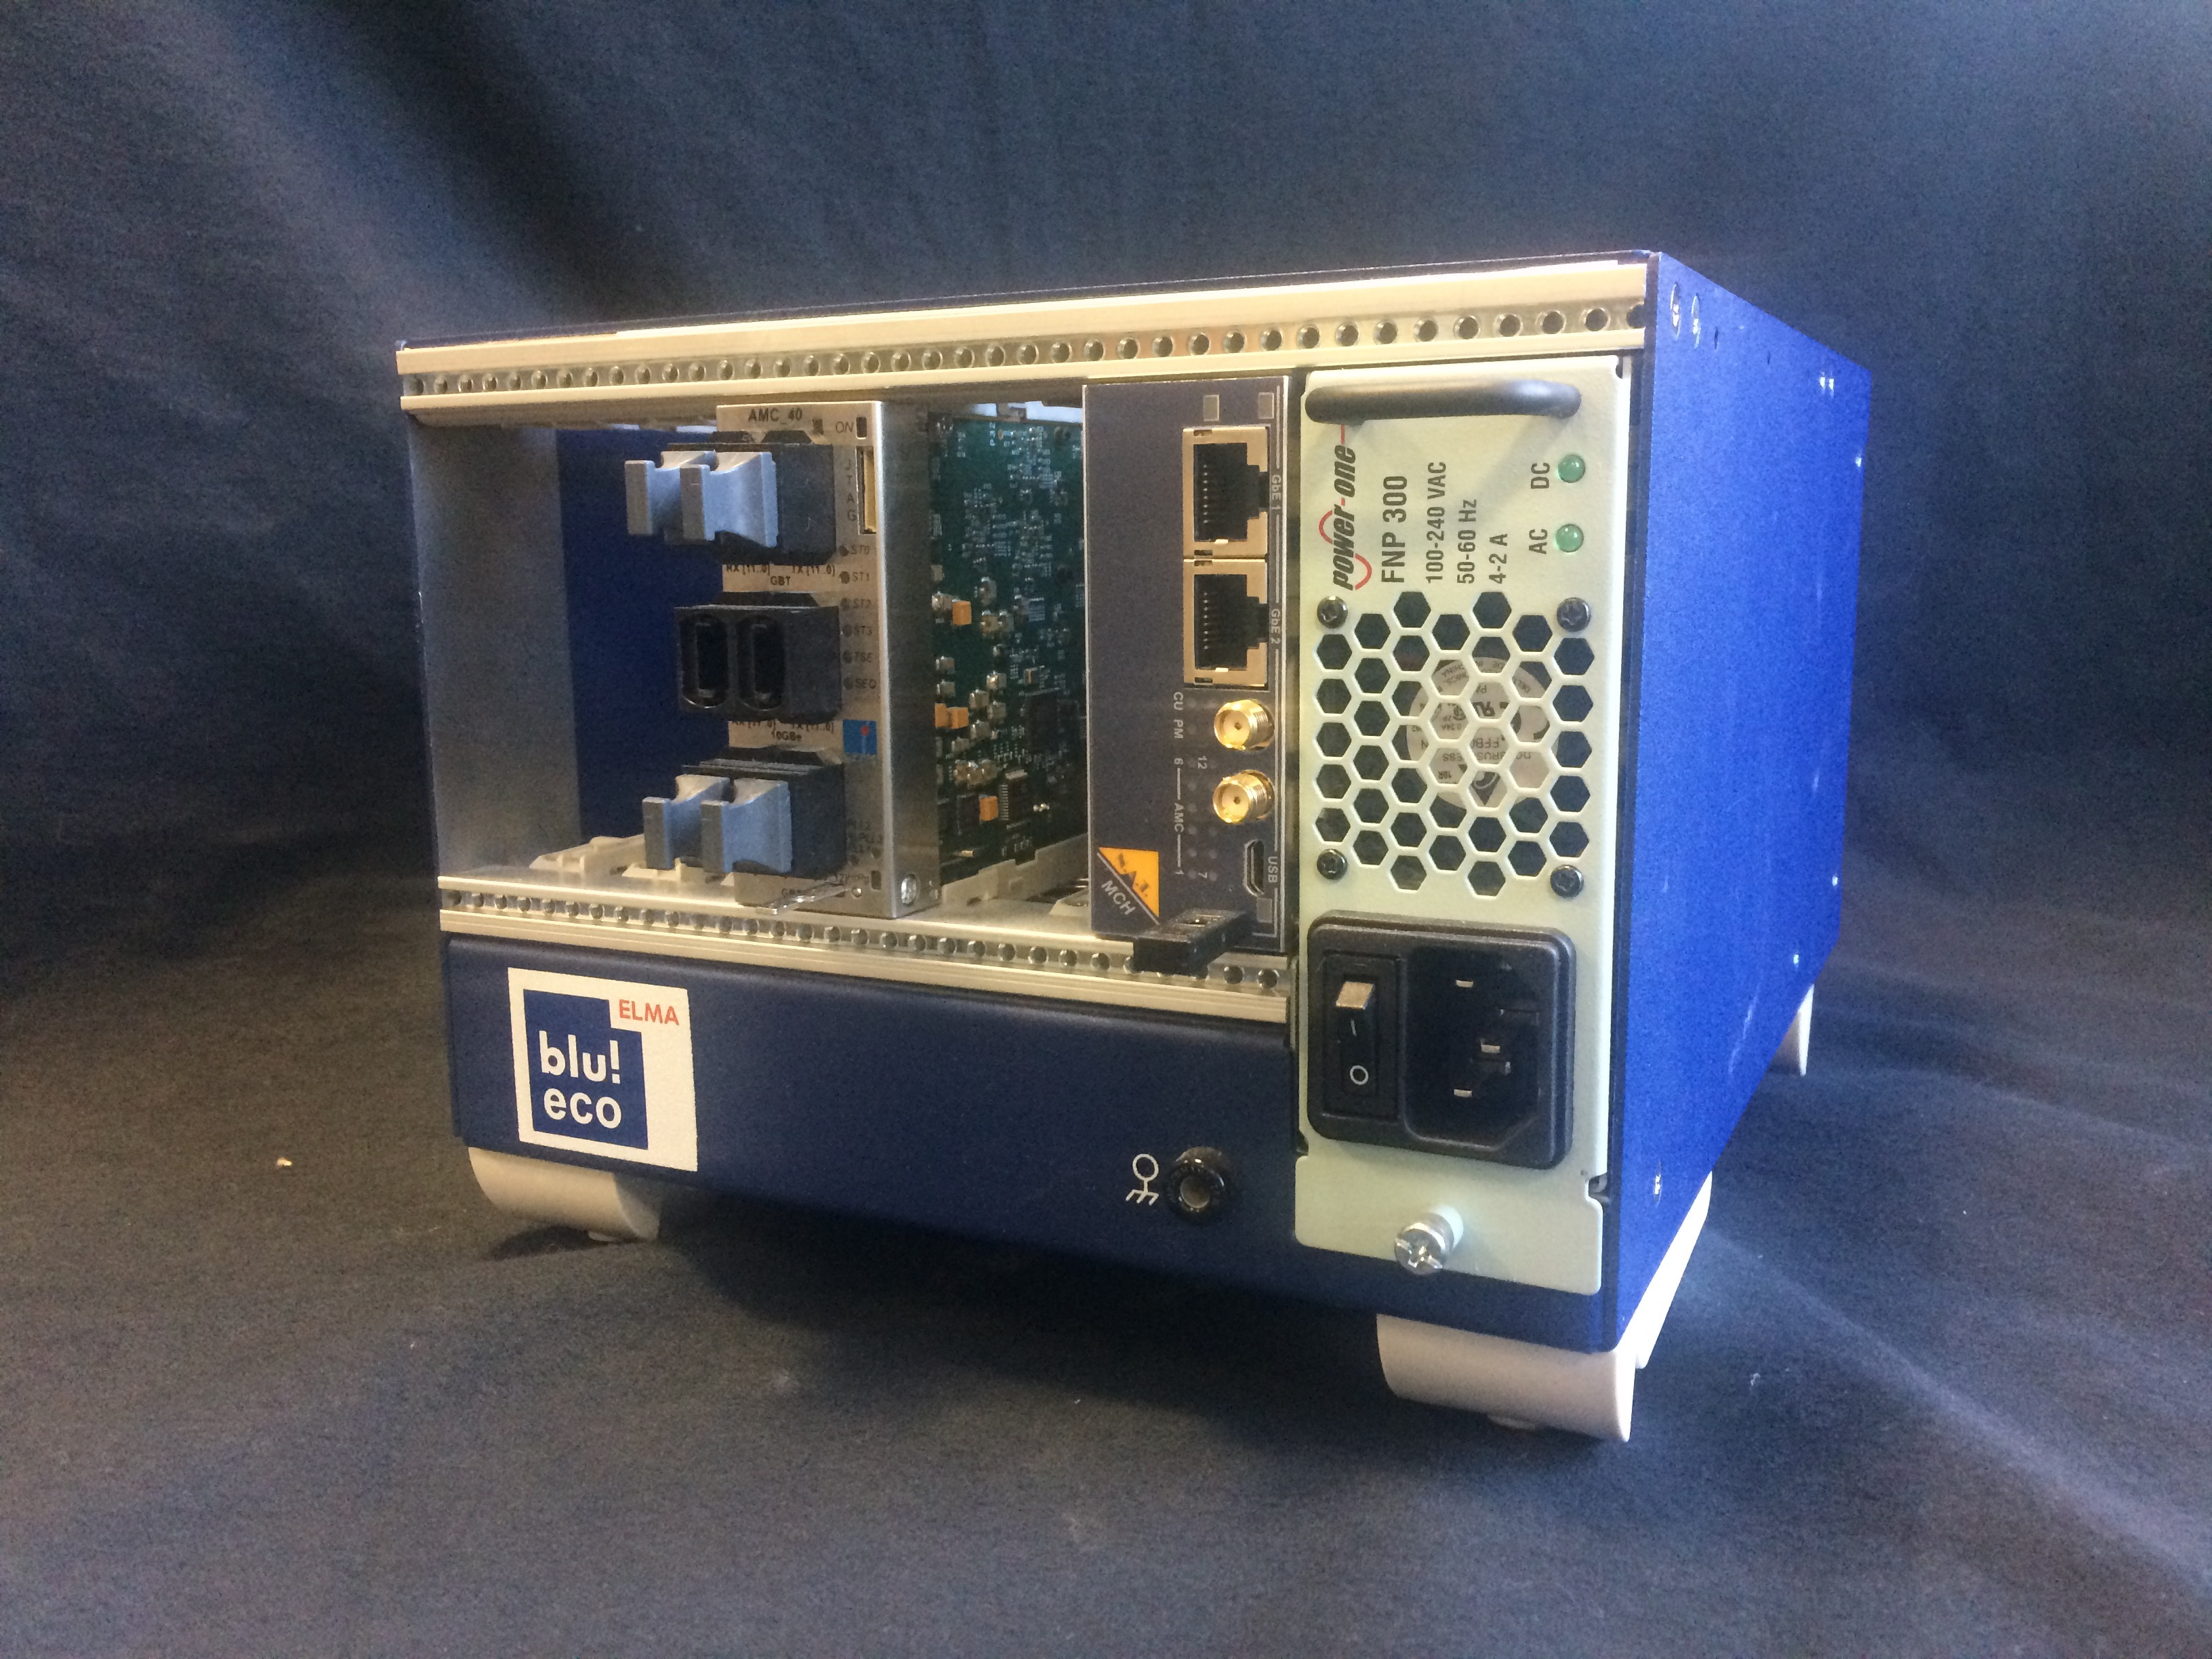
\includegraphics[width=\linewidth]{03_GraphicFiles/chapter3_CLaRySproto/Electronics_Acquisition/uTCAcrate_1.jpg}
\caption{\gls{utca} crate with the \gls{amc}40 board.}
\label{chap3::fig::uTCAcrate}
\end{subfigure}
\begin{subfigure}[htbp]{.41\textwidth}
\centering
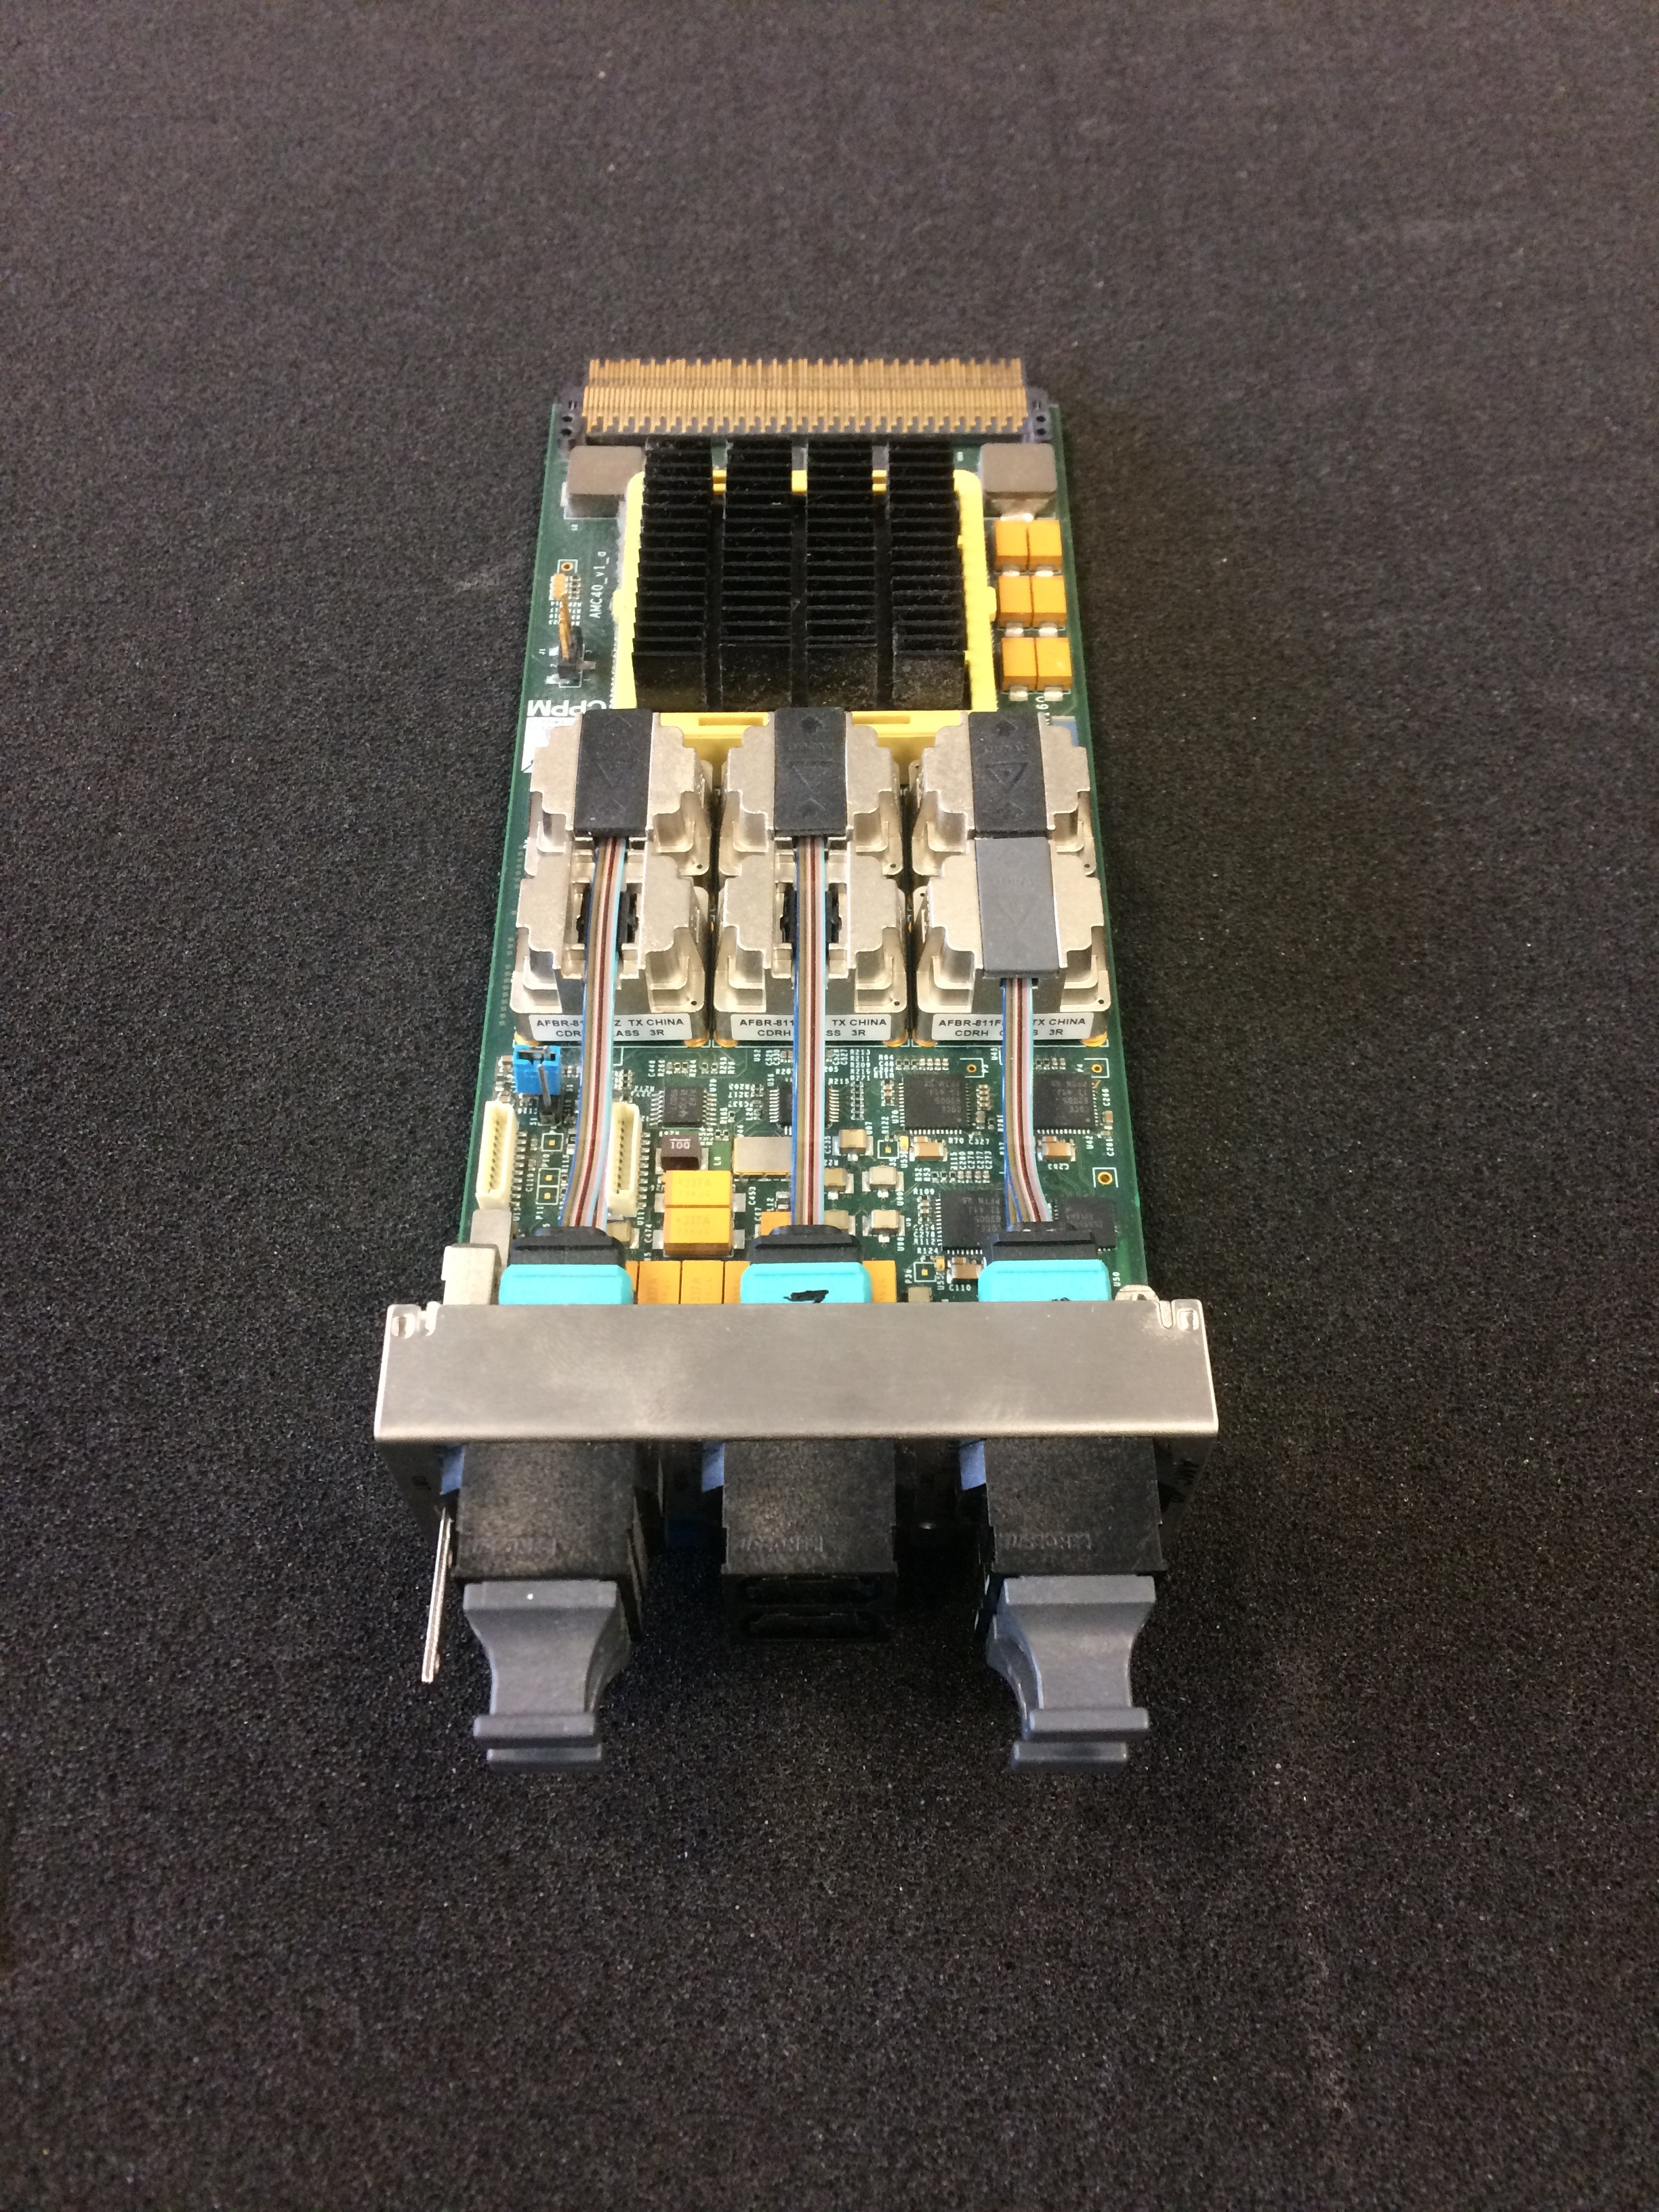
\includegraphics[width=\linewidth, angle = -90]{03_GraphicFiles/chapter3_CLaRySproto/Electronics_Acquisition/AMC40_ipnl_top.jpg}
\caption{\gls{amc}40 board.}
\label{chap3::fig::AMC40}
\end{subfigure}
\newline
\begin{subfigure}[b]{\textwidth}
\centering
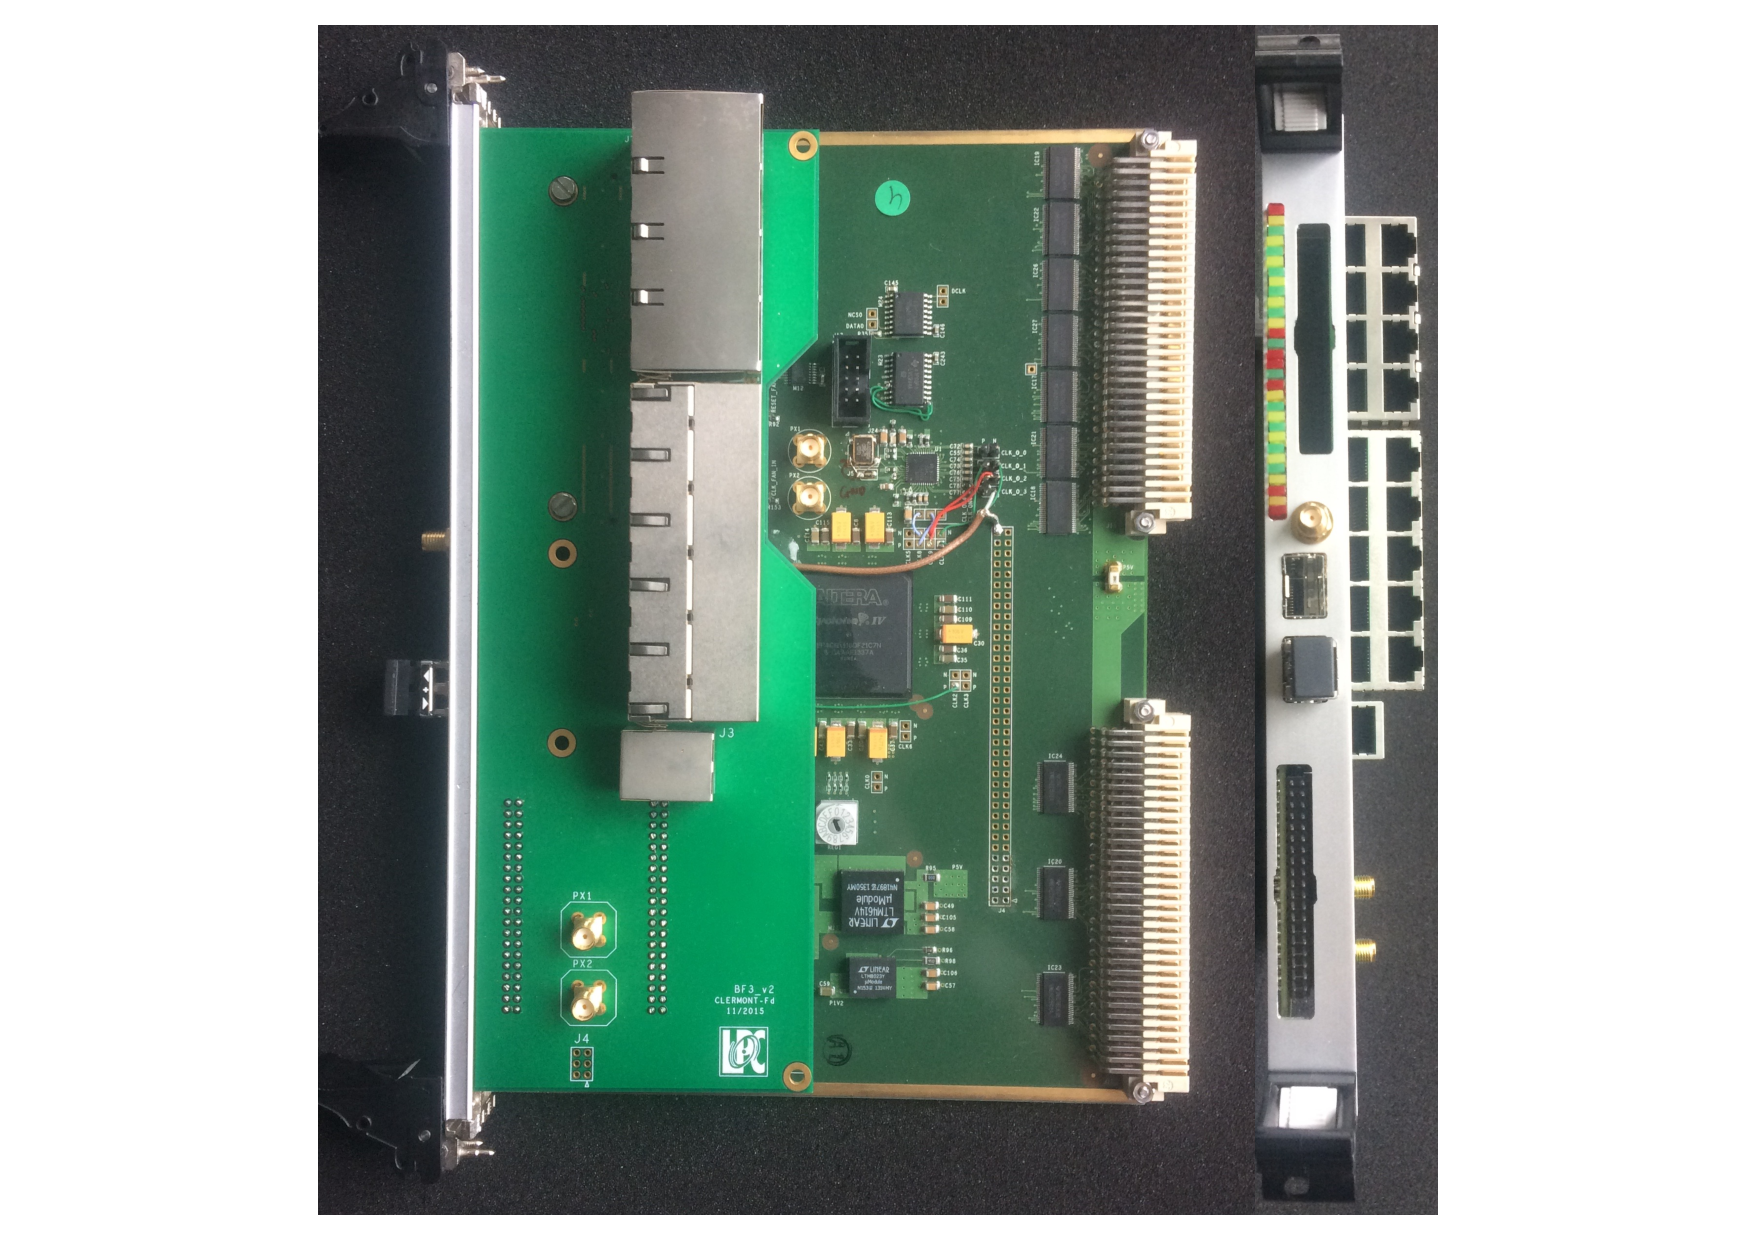
\includegraphics[width=0.8\linewidth]{03_GraphicFiles/chapter3_CLaRySproto/Electronics_Acquisition/THOR.pdf}
\caption{\gls{thor} card.}
\label{chap3::fig::THOR}
\end{subfigure}
\caption{Acquisition system components: \gls{utca} crate (a), \gls{amc}40 board (b) and \gls{thor} card (c).}
\label{chap3::fig::AcquisitionSystem}
\end{figure}


For both cameras, the acquisition starts in case the absorber section detects an interaction: the \gls{asm} involved card deals with the creation of a pre-trigger signal, which corresponds to the digital output signal and contains a time stamp (see the \gls{asm} card description in section~\ref{chap3::subsubsec::AbsorberFEcard}). The pre-trigger is sent to the \gls{thor} card who governs its distribution to the other system components.\\ 
In the multi-slit collimated camera, the pre-trigger signal directly operates as a trigger validating the data collection from absorber and hodoscope. In the Compton camera, the \gls{thor} card initially sends the pre-trigger to the scatterer \gls{fe} cards, which explore their buffer looking for events in the coincidence time window; if a coincidence is found, a trigger signal is generated by the scatterer \gls{fe} card and sent to the acquisition system, which then starts the data read-out from all the detectors. An graphical overview of the complete acquisition system and logic is given in \figurename~\ref{chap3::fig::DAQscheme}.\\
The \gls{amc}40 card makes use of three buffers for the three detector sections, where the collected data are stored until the creation of packets of the selected size to be sent to the acquisition PC. The data transfer is achieved via a 1~Gbit/s Ethernet link, and the chosen standard is the \gls{udp}. The data format has been fixed at the camera conception stage and slightly modified following the electronics developments; it is deeply described in the appendix~\ref{chap::appA}, which also reports the expected data flow obtained in previous simulation studies.\\  
In addition to the already explained functions, the \gls{utca} is also in charge of handling the slow control signals for the configuration of the detector \gls{fe} cards. The chosen format is in this case the \gls{tcp}, which is more reliable and ensures a feedback in case of communication failure. The possible slow control signals are detailed in appendix~\ref{chap::appA}.\\

\begin{figure}[!htbp]
\centering
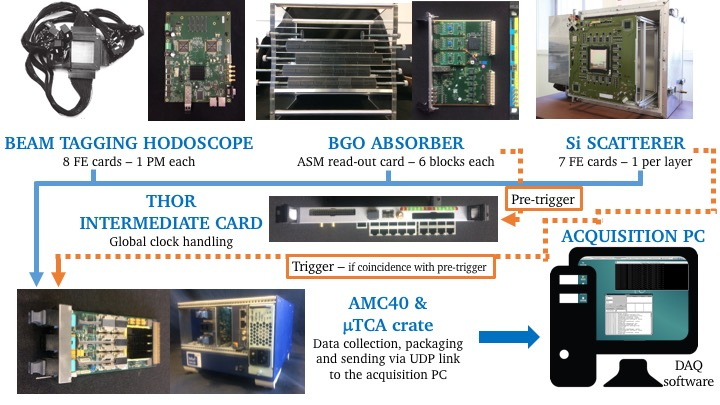
\includegraphics[width=\textwidth, trim = {0 2cm 0 2cm}, clip = true]{03_GraphicFiles/chapter3_CLaRySproto/Electronics_Acquisition/acqLogic_complete.pdf}
\caption{Schematic view of the Compton camera acquisition system. For the multi-collimated camera, the trigger and pre-trigger signals are the same.}
\label{chap3::fig::DAQscheme}
\end{figure}

%%%%%%%%%%%%%%%%%%%%%%%%%%%%%%%%%%   SOFTWARE  %%%%%%%%%%%%%%%%%%%%%%%%%%%%%%%%%%%%%%%%%%%%

\subsection{Camera acquisition, monitoring and slow control software}\label{chap3::subsec::cameraSoftware}

The \gls{udp} data packets sent by the \gls{utca} acquisition system via Ethernet link are received by the acquisition PC thanks to a C++ based acquisition software, developed at the \gls{ipnl}. The software decodes the data packets and builds the events by grouping the data from the two (for the multi-slit collimated camera) or three (for the Compton camera) detection sections according to the time stamp. During the decoding process, the software also verify the received data format and can highlight problems in the data encoding by the \gls{utca}; this feature is used during the test phase to check the functionality of the \gls{amc}40 firmware. The reconstructed events are then stored in binary files with the structure presented in appendix~\ref{chap::appA}. The data file size can be selected by fixing the number of events stored per run in the acquisition run, knowing that each event can be composed by slightly different number of bits, according to the amount of detector modules involved. The file collection corresponding to the same run will be then grouped at the analysis stage. The number of events per file must be tuned taking care of the available \gls{ram} (32~Gb), where the data are temporarily stored before the writing process on the hard-disk. In \figurename~\ref{chap3::fig::daqSoftware} the minimal graphical interface developed for the acquisition software is shown.\\

\begin{figure}
\begin{subfigure}[t]{.5\textwidth}
\centering
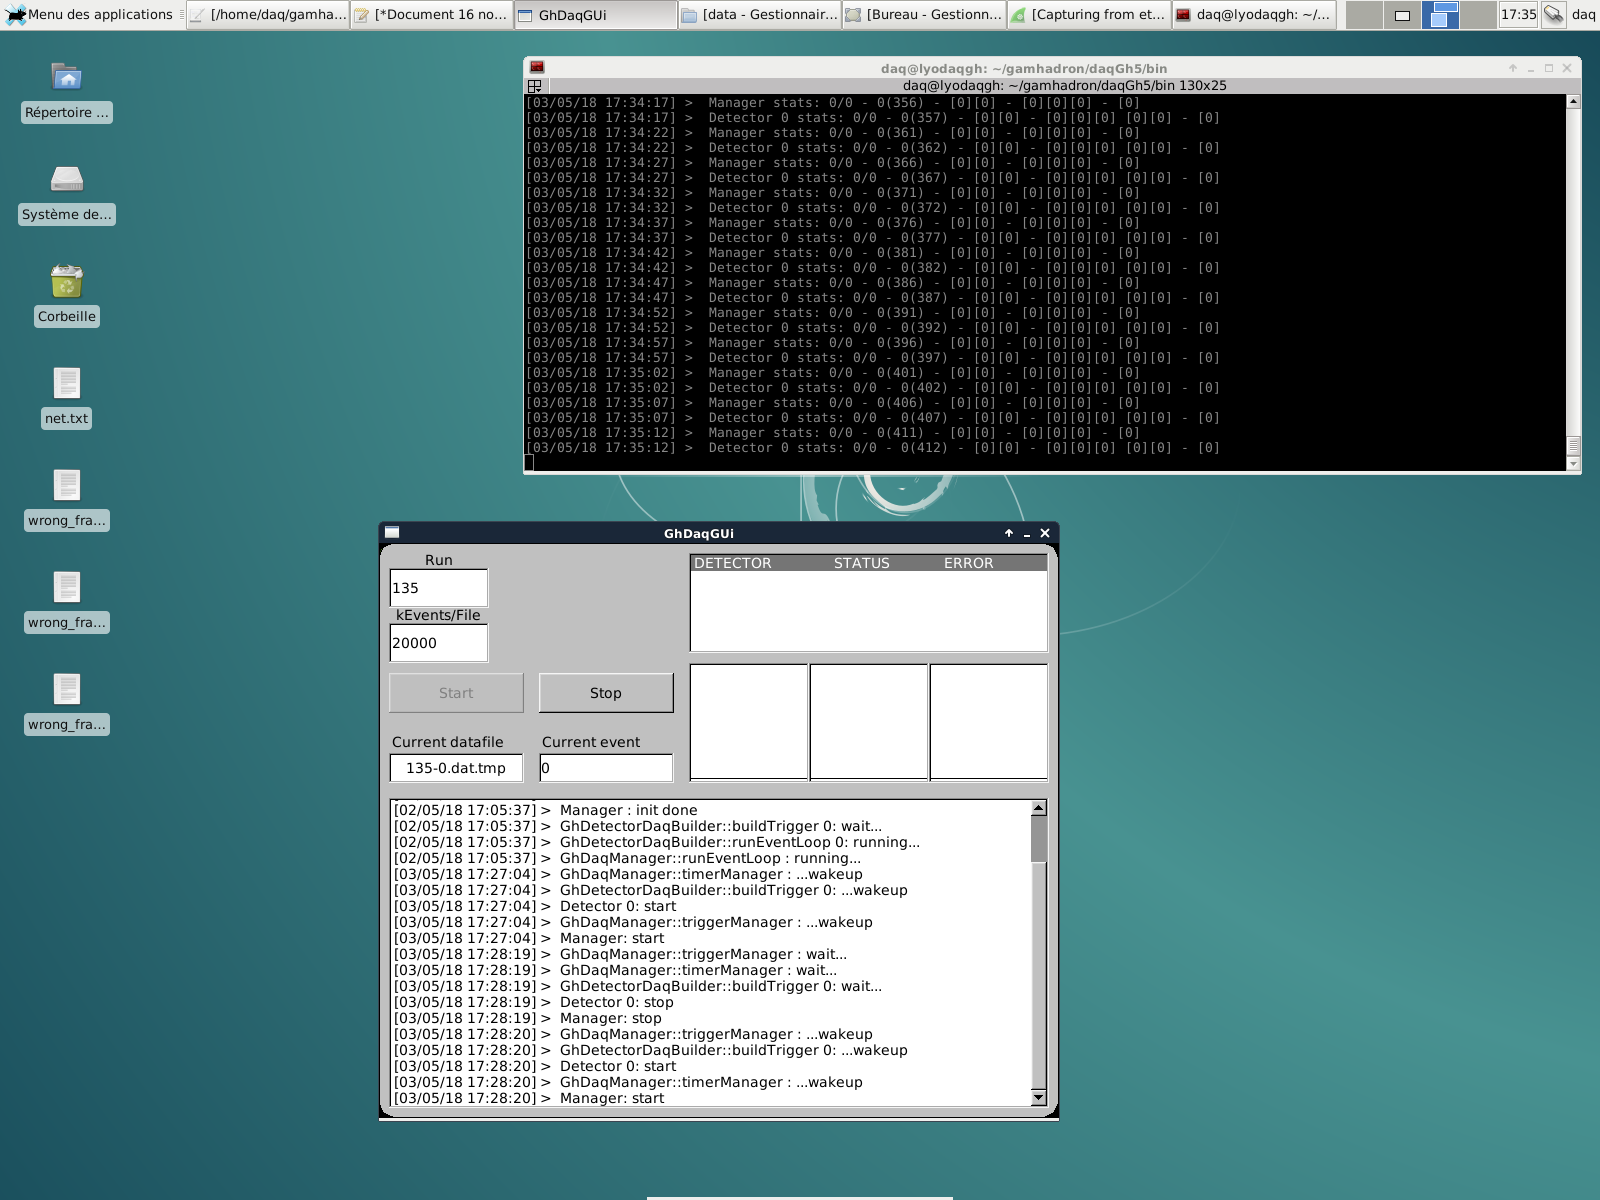
\includegraphics[width=0.75\textwidth]{03_GraphicFiles/chapter3_CLaRySproto/Electronics_Acquisition/DAQsoft.png}
\caption{Acquisition software user interface.}
\label{chap3::fig::daqSoftware}
\end{subfigure}
\begin{subfigure}[t]{.5\textwidth}
\centering
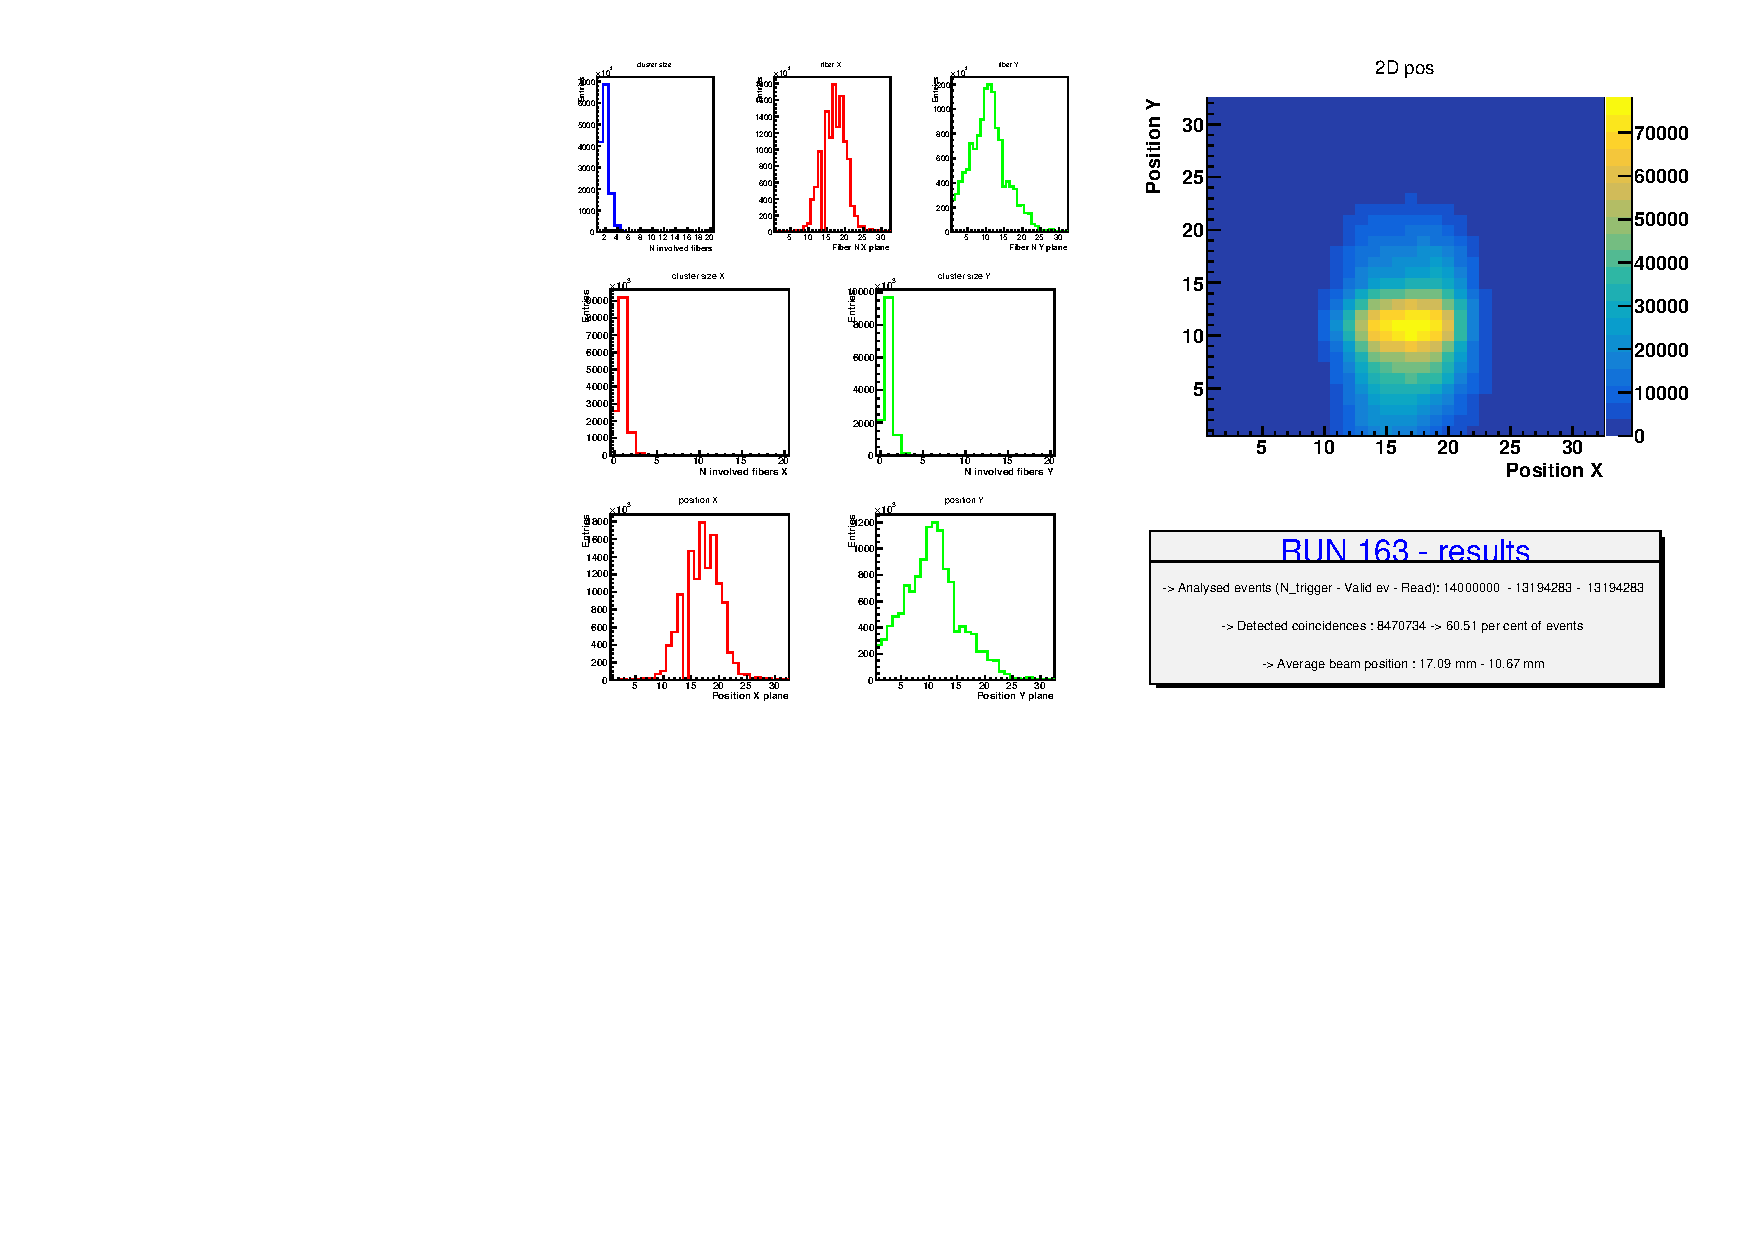
\includegraphics[width=1\textwidth]{03_GraphicFiles/chapter3_CLaRySproto/Electronics_Acquisition/monitoringEx.pdf}
\caption{Example of monitoring software visualization for the beam tagging hodoscope (applied to the 32$\times$32 fiber prototype).}
\label{chap3::fig::monitoringSoftware}
\end{subfigure}
\caption{Software tools: user interface of the acquisition C++ software (a) and example of the ROOT monitoring software visualization for the beam tagging hodoscope 32$\times$32 fiber prototype.}
\label{chap3::fig::SoftwareAll}
\end{figure}

A monitoring software has been developed in order to have a direct real-time feedback on the camera data acquisition. The software can show some information about the ongoing data collection, and it is at present designed to work on a single detector section (hodoscope, scatterer or absorber). It is based on ROOT with the following working logic: during the acquisition, it continuously searches for new data files in the storage folder, and analyses in the desired way a selected number of events per file, directly from the binary format. An example of the visualized output for an hodoscope monitoring is shown in \figurename~\ref{chap3::fig::monitoringSoftware}. This picture corresponds to an acquisition performed during a beam test at the \gls{cal}, where the 32$\times$32 fiber hodoscope have been tested, together with the monitoring software. More details about the beam test are given in chapter~\ref{chap::6}.\\ As mentioned, the present version of the software is not yet adapted to the monitoring of the whole camera, even if it can handle at least two detectors with minor modifications. In addition to this, it is not automatically synchronized with the acquisition software, and not optimized in terms of needed calculation time. In the next future the planned upgrade will slightly modify the working logic by directly connection the monitoring to the acquisition: the acquisition software will automatically send a selected fraction of events to the monitoring output during the acquisition, so that the search for data files would not be anymore necessary. This will drastically reduce the monitoring dead time and calculation time, achieving an actual online control.\\
Acquisition and monitoring software has been tested thanks to a data simulator developed in C++, which is able to create data \gls{udp} packets with the correct format and send them on the same Ethernet port used for the data collection, simulating a server-client communication.\\

As mentioned in section~	\ref{chap3::subsec::cameraElectronicsDAQ}, the \gls{utca} handles both the data collection and transfer and the slow-control of the whole system, where with slow-control we intend the configuration of all the electronics cards (discriminator thresholds, channel gains, \gls{asic} reset signals, working mode, etc.) and the read-out of the feedback signals. The development of the slow-control software is ongoing at the \gls{ipnl}: it is designed in LabVIEW and includes all the needed controls in a single user interface. A dedicated PC is foreseen for this task, connected to the \gls{utca} via \gls{tcp} protocol. The slow-control software will also govern the high and low voltage suppliers for the detectors and acquisition electronics boards, the scatterer thermal box temperature setup and control, the steering of the 2D positiong table dedicated to the hodoscope, and the steering of the camera moving table, described in the next section. All the listed instruments will be connected to a patch panel, and a local network will be created for the camera equipment.      

%%%%%%%%%%%%%%%%%%%%%%%%%%%%%%%%%%   MECHANICAL SUPPORT  %%%%%%%%%%%%%%%%%%%%%%%%%%%%%%%%%%%%%%%%%%%%

\subsection{Camera integration and mechanical support}\label{chap3::subsec::CameraMechanics}

In order to setup the two camera configurations (multi-slit and Compton), the described components, together with the related mechanical supports, must be integrated in an integral system, with the exception of the beam tagging hodoscope who has its own dedicated mechanical support, being placed between the beam nozzle and the target. A general mechanical structure is then needed to support the camera; it is required to be movable, as compact as possible but at the same time robust and large enough to support absorber and scatterer (or collimator), for a total maximum weight of about 100~Kg. In addition to this, it should be possible to remotely control the position of the various camera components in order to adapt their position in 3D with respect to the beam line and to the target.\\
The realized solution is shown in \figurename~\ref{chap3::fig::pictureTable}. It is composed of two sections: a positioning table on wheels, designed and provided by Rose \& Krieger, equipped with 4 telescopic feet, and a 4-axis moving table installed on it, developed by Kinetic System. The wheels allow to first position the camera, and the 4 telescopic feet are used to regulate with 1~mm precision the whole system height, in the range 630~mm - 1280~mm from the ground, to be adapted to the specific beam line. The feet are expected to be able to support a maximum weight of 150~Kg. The telescopic feet are not connected to the slow-control but are controlled by a remote controller on the table itself. On the top surface of the table, 1200$\times$750~mm$^2$, the 4-axis moving table is fixed and allows to adapt the camera position in 3D (distance camera-target, height, direction parallel to the beam line) with a 100~\charmum resolution and a range of 40~cm. In addition to this, a fourth axis allows to adjust the distance between the two detector components in the direction perpendicular to the beam line, in a range of 30~cm (to be noticed that this range is reduced by the size of the scatterer thermal box). The four axes are connected to the positioning table patch panel, which is directly controlled by the slow-control program in LabVIEW. Finally, a further manual control allows to rotate the whole system with respect to the table axis, in a range of $\varpm$ 10 degrees.\\
In \figurename~\ref{chap3::fig::schemeTable} we present the mechanical scheme of the complete positioning table, with the Compton camera installed on it.\\ 

\begin{figure}
\begin{subfigure}[t]{.5\textwidth}
\centering
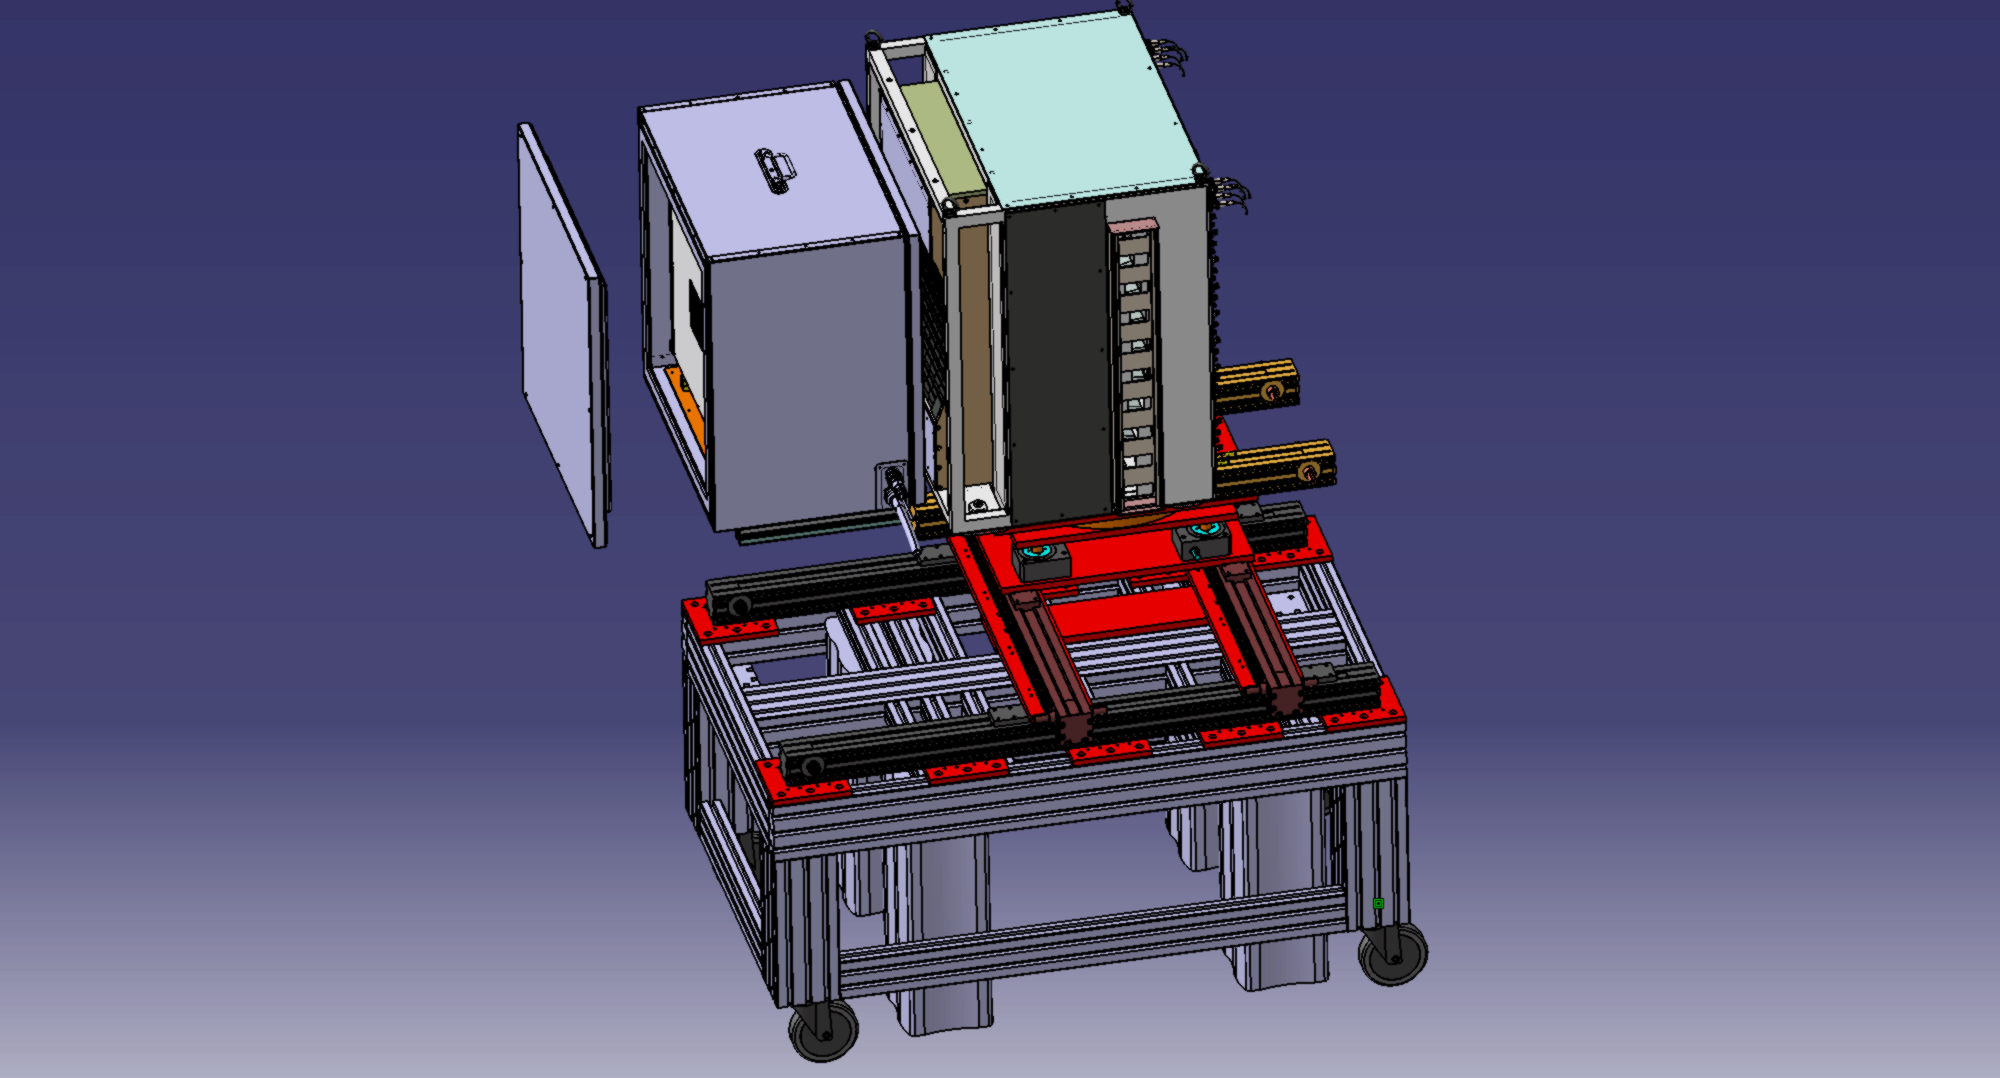
\includegraphics[width=1\textwidth, trim= {1cm 0 1cm 0}, clip = true, height=5cm]{03_GraphicFiles/chapter3_CLaRySproto/Mechanics/TableCameraSchemeBlue.jpg}
\caption{Schematic view of the Compton camera integration on the positioning table.}
\label{chap3::fig::schemeTable}
\end{subfigure}
\begin{subfigure}[t]{.5\textwidth}
\centering
\includegraphics[width=1\textwidth]{03_GraphicFiles/chapter3_CLaRySproto/Mechanics/Table.JPG}
\caption{Gamma camera position table.}
\label{chap3::fig::pictureTable}
\end{subfigure}
\caption{Details of the gamma camera integration and mechanical support.}
\label{chap3::fig::CameraIntegration}
\end{figure}

In \figurename~\ref{chap3::fig::cameraAllPicture} we show a view of the three detectors composing the Compton camera, with one scatterer layer installed in the thermal box and the absorber mounted on the positioning table, and the beam tagging hodoscope on the right side on its dedicated mechanical support.\\

\begin{figure}[!htbp]
\centering
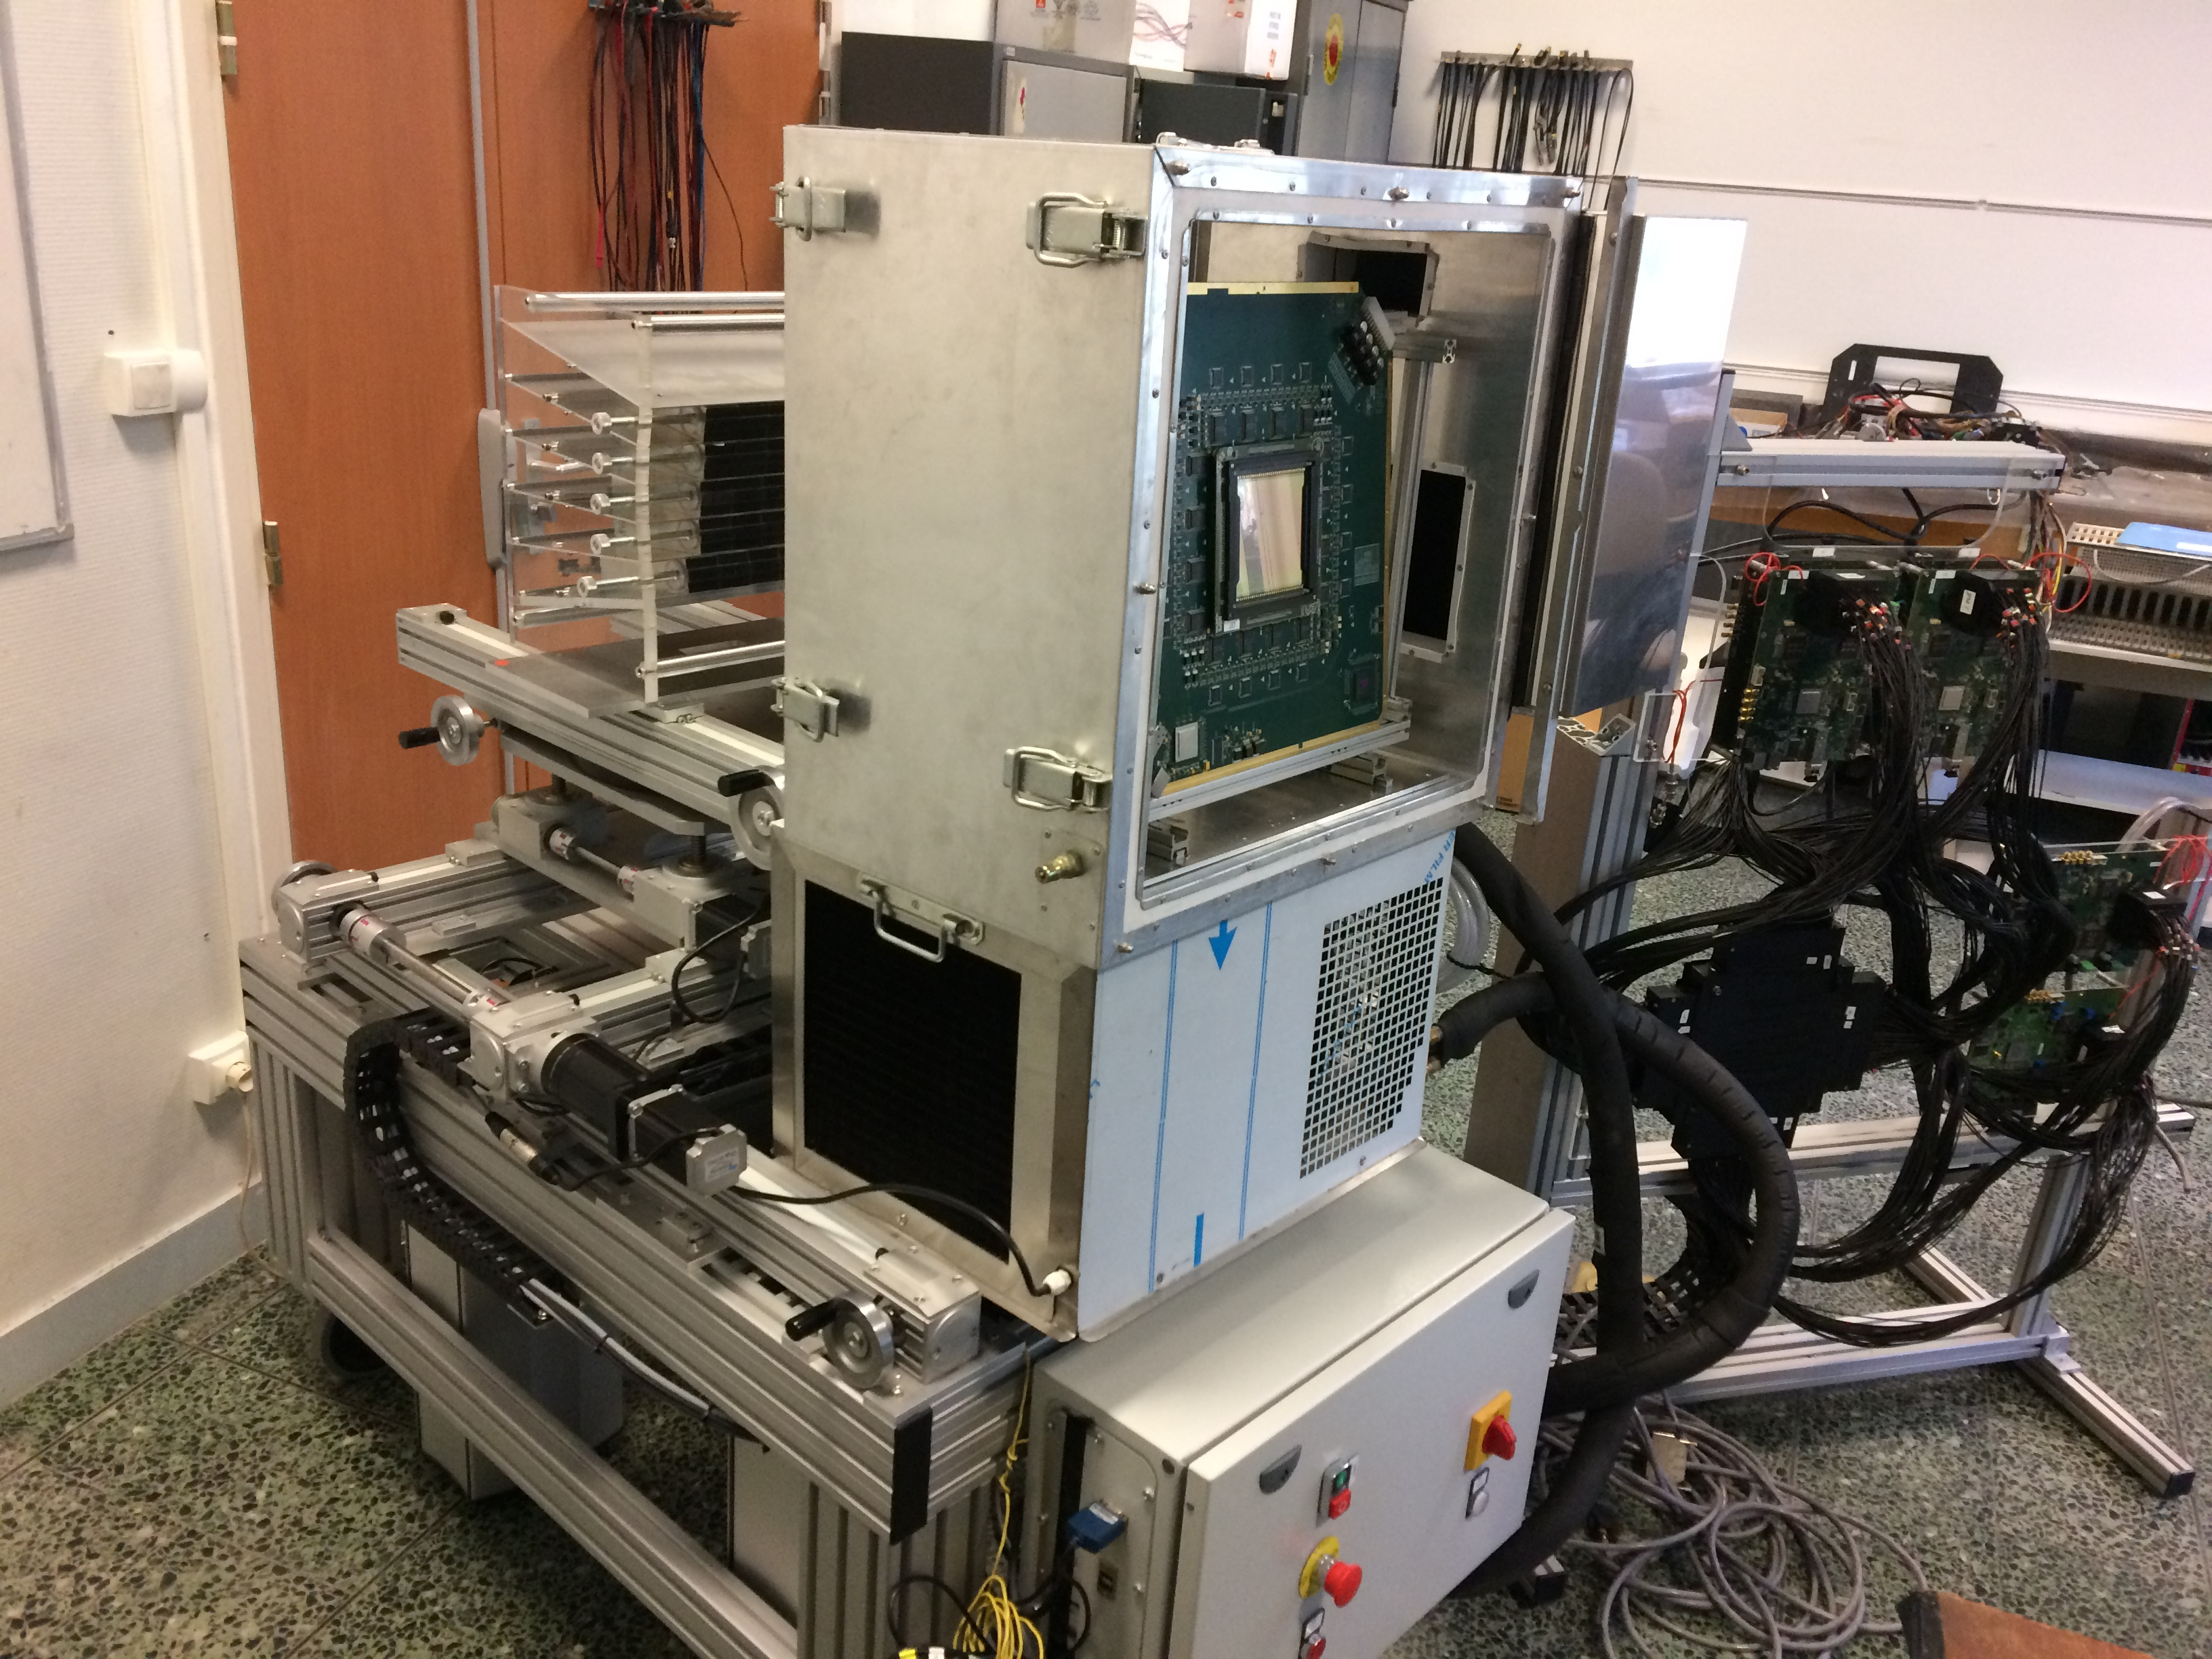
\includegraphics[width=\textwidth]{03_GraphicFiles/chapter3_CLaRySproto/camera_complete.JPG}
\caption{Complete Compton camera with beam tagging hodoscope on the developed mechanical supports.}
\label{chap3::fig::cameraAllPicture}
\end{figure}

\newpage

%%%%%%%%%%%%%%%%%%%%%%%%%%%%%%%%%%   CHARACTERIZATION MEASUREMENTS  %%%%%%%%%%%%%%%%%%%%%%%%%%%%%%%%%%%%%%%%%%%%

\section{Camera component characterization and development status}\label{chap3::sec::charMeasurements}

As detailed in the previous sections, the \gls{clarys} \gls{tof} gamma cameras are equipped with various detector components with very different features. Each part must be separately studied in order to characterize its behavior and allow the final camera integration and operation.\\
I mostly worked on the beam tagging hodoscope and on the \gls{bgo} absorber, and in the next paragraphs the performed measurements are described in details. Concerning the scatterer stack, the results achieved before the beginning of my PhD thesis are briefly described for the sake of completeness.\\
The results presented in this section also introduce the following one (~\ref{chap3::sec::Next}), where all the development steps still needed for a clinical implementation of the cameras are explained.\\

\subsection{Scatterer silicon layer characterization}\label{chap3::subsec::scattSichar}


\newpage

\subsection{Absorber \gls{bgo} blocks characterization}\label{chap3::subsec::absBGOchar}

The \gls{bgo} modules composing the Compton and multi-collimated camera absorber have been recovered form a SIEMENS \gls{pet} system: they have been originally optimized for the detection of 511~keV photons from positron annihilation, and they have to be tested for the new gamma detection system, which must be able to deal with photons in the prompt-gamma energy range, i.e.~from some hundreds of keV to a few MeV.\\ 
Each block must be characterized in terms of spatial and energy response, and the read-out \glspl{pm} have to be calibrated to obtain a uniform response on the whole block surface (see section~\ref{chap3::subsec::absorber} for the detector description). The employed method relies on the work presented in~\cite{Rogers1994} and~\cite{Tornai1994} and on the calibration process described in~\cite{Golnik2015} and~\cite{HuesoGonzalez2015}, and has been extended with more refined features.\\
The measurements are performed with the irradiation with gamma sources, emitting photons at defined energies: in particular, we used 511~keV and 1275~keV photons from a $^{22}$Na source, and the two photons emitted by a $^{60}$Co source, at energies of 1173~keV and 1332~keV.\\
The employed $^{22}$Na source is a cylindrical source with a diameter of 1~cm, and an activity of about 400~kBq: it has been placed at a distance of about 5~cm from the block entrance surface, with the center of the source facing the center of the block transverse surface. The $^{60}$Co source has been installed in a lead cylindrical container (12~cm radius and 35~cm height), equipped with three different apertures: point-like (2$\times$2~mm$^2$), linear (2$\times$50~mm$^2$) and squared (50$\times$50~mm$^2$). The design of the lead container has been studied in simulation to ensure the proper radiation protection, and produced according to the specifications defined by the \gls{ipnl} mechanics group. The activity of the $^{60}$Co source is about 1.7~MBq, and the square shape has been used to obtain an homogeneous irradiation of the \gls{bgo} block, with the block set with the center of the entrance surface corresponding to the source position, at a distance of 12~cm.\\
The signals produced by the four \glspl{pm} of each block are collected via four analog outputs on the front-end card (see picture~\ref{chap3::fig::FEcard}). The four retrieved signals per event are treated via standard \gls{nim} modules in order to be adapted to the acquisition systems and measurement purposes.\\
Two different acquisition systems have been used for this characterization work. First, the PXIe described in section~\ref{chap3::subsec::hodoPMchar} with its two flash \gls{adc} read-out modules, 8 channels each, is used for the spatial and energy characterization and calibration of the tested blocks. The raw signals coming from the four \glspl{pm} are amplified and shaped via \gls{nim} modules, which have been fine tuned via a pulse generator in order to adapt the amplification factor of each channel (an amplification factor of about 50 has been applied to the raw signals). The amplified signals are then split in order to be treated for trigger purpose. The trigger for the acquisition is based on the sum of the four signals, and a fixed threshold is applied for background rejection. The employed discriminator provides the logical trigger signal, which is sent to the trigger input of the \gls{adc} modules on the PXI. The four amplified signals, conveniently delayed, are sent as inputs to the \gls{adc} modules on the PXI, together with the sum signal which is used for experimental verification of the acquisition setup. A LabVIEW based acquisition software, developed for this particular application by the \gls{ipnl} group, provides real time event visualization together with a partial, on-line spatial reconstruction of the events, and stores them in text files for further analysis. A second threshold can be set at the software level in case particular selections are needed during the acquisition, otherwise the event selection is performed at the analysis stage.\\
Concerning the timing characterization measurements, an eight-channel signal digitizer at 3.2~GS/s has been employed for high time resolution acquisitions. The so-called WaveCatcher, shown in \figurename~\ref{chap3::fig::WaveCatcher}, has been developed by the \gls{lal} in Orsay and the \gls{irfu} in CEA-Saclay, and its features are detailed in~\cite{Breton2014}. The digitizer is connected to the acquisition PC via \gls{usb} cable, and the data read-out and storage is performed thanks to a custom acquisition software.  The measurements are based on the coincidence detection of back-to-back 511~keV photons emitted by a $^{22}$Na radioactive source, in order to be able to compare the time response of the tested \gls{bgo} block to a reference fast timing scintillator. An external trigger is then provided to the WaveCatcher by treating the \gls{bgo} block and reference scintillator signals with logic coincidence \gls{nim} modules, after proper discrimination. Further details are given in section~\ref{chap3::subsubsec::absTimeMethod}.

\begin{figure}
\begin{subfigure}[t]{.45\textwidth}
\centering
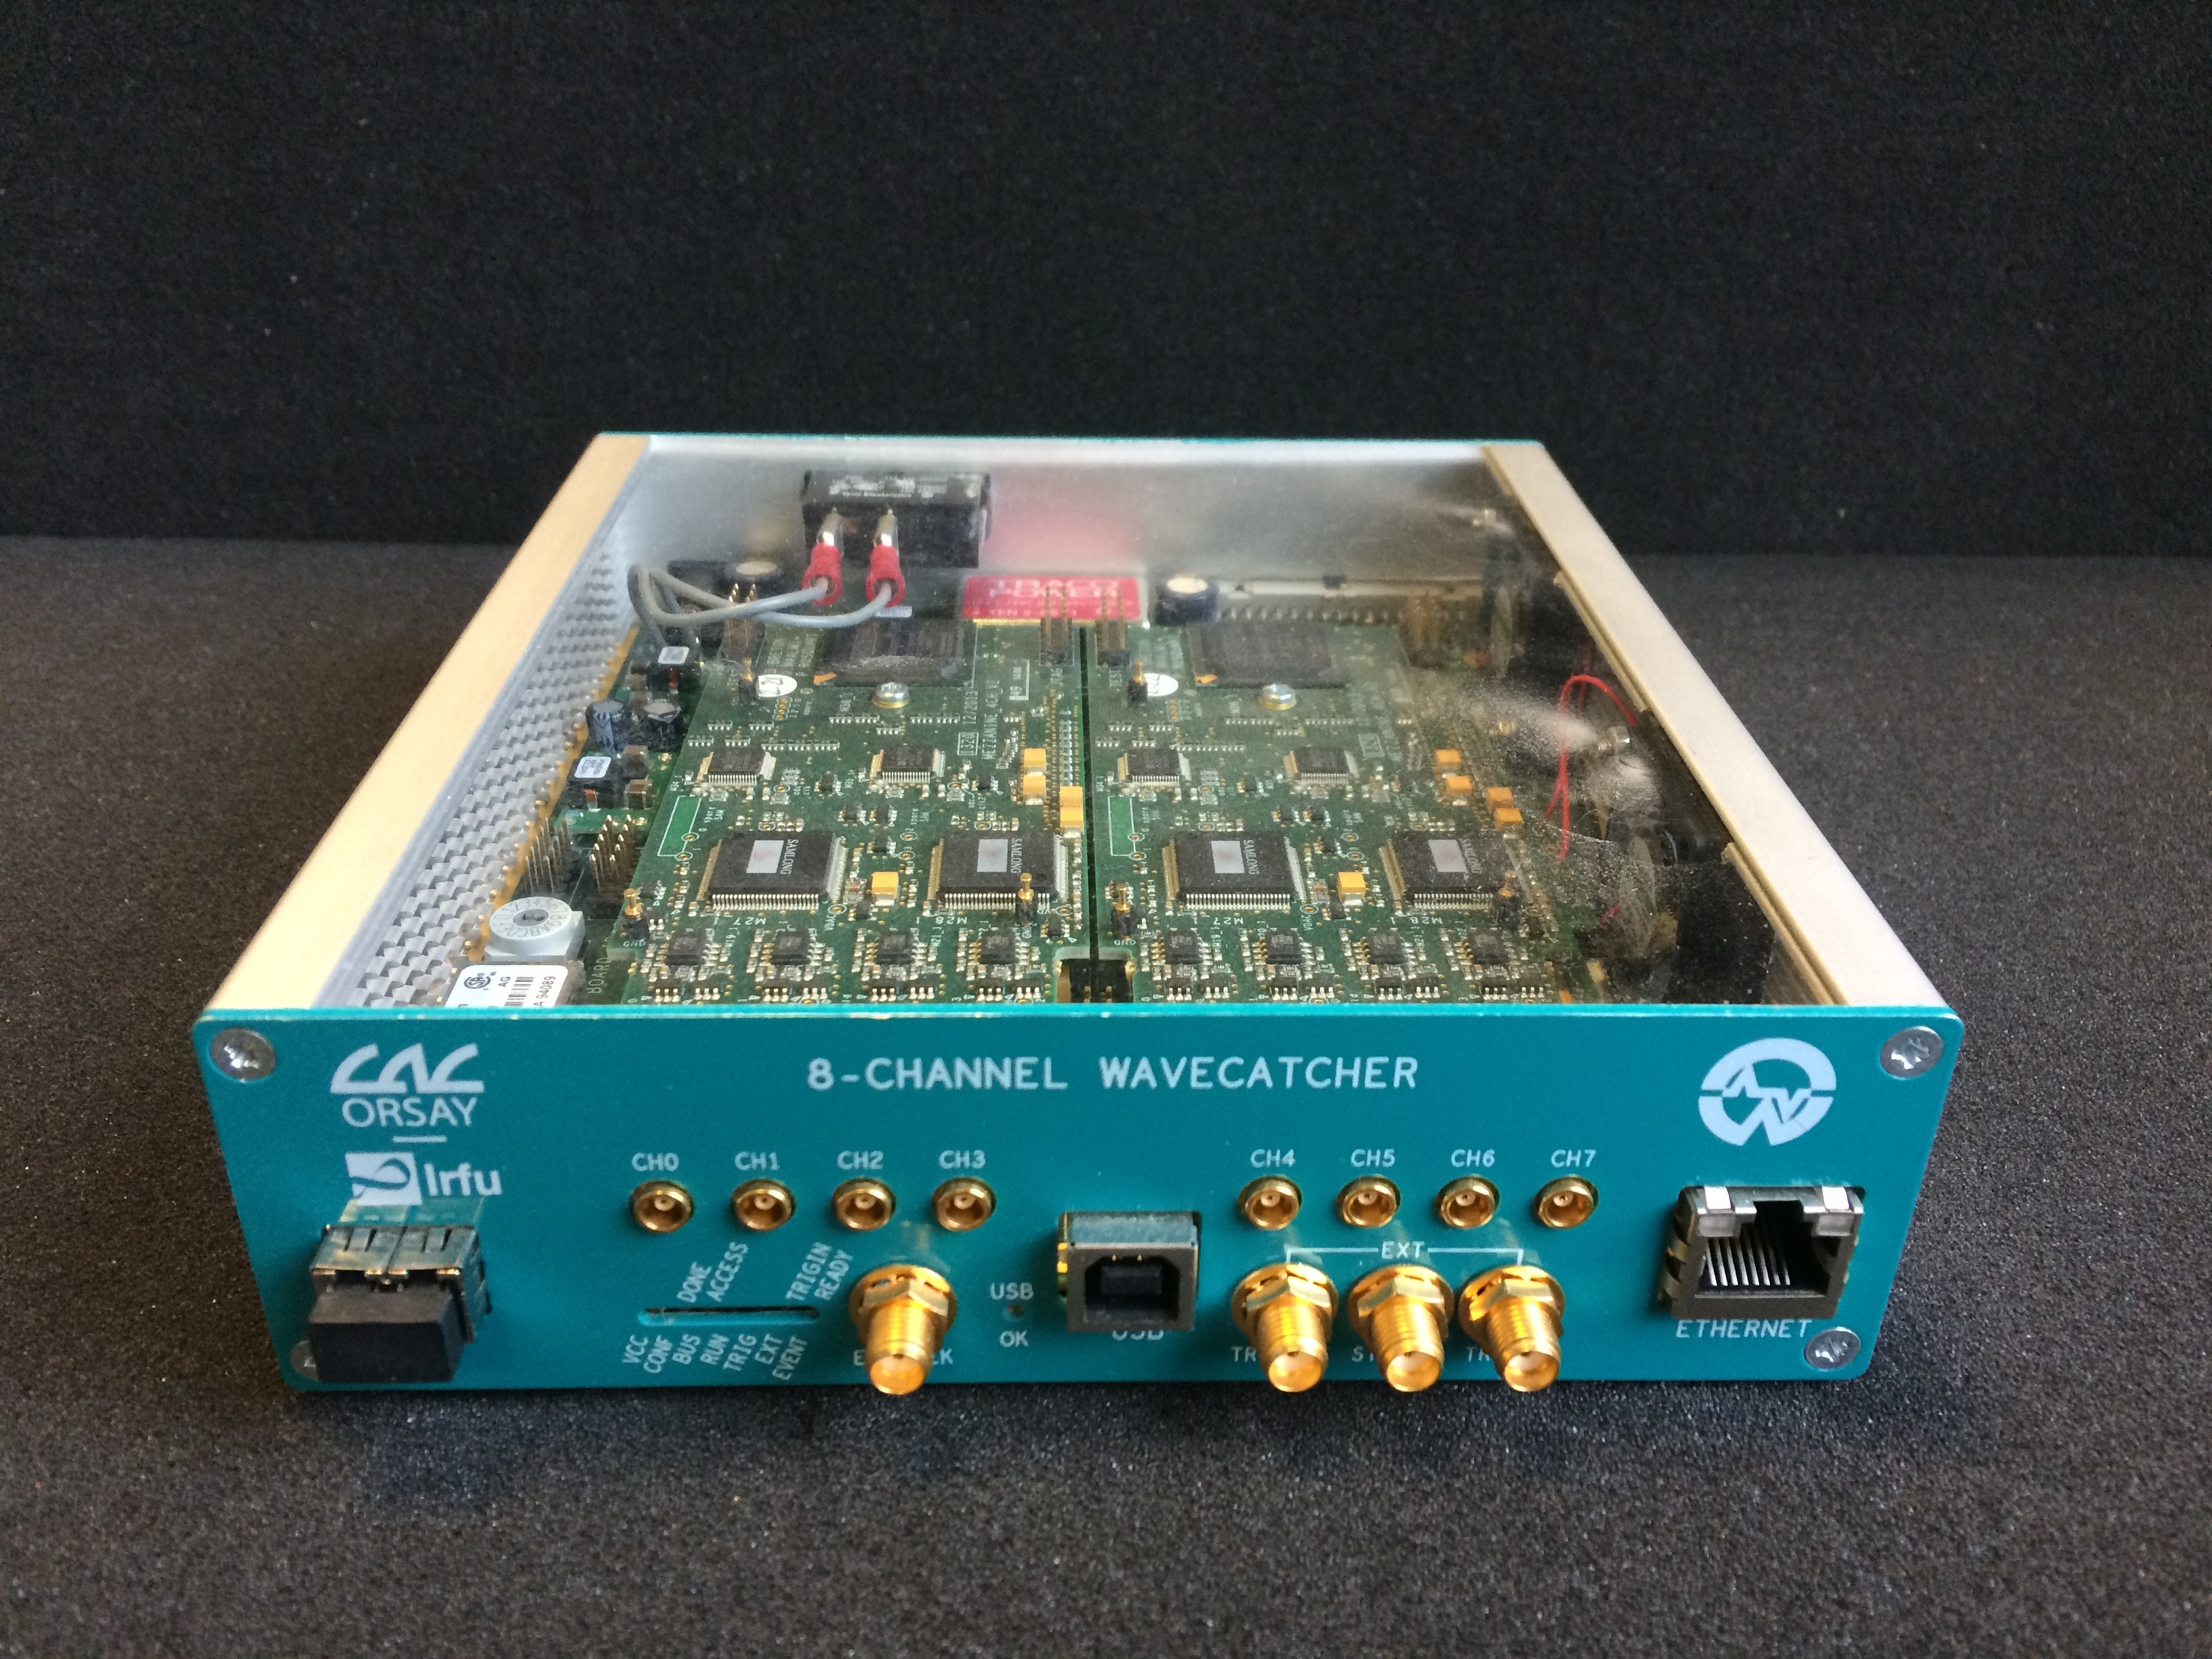
\includegraphics[width=1\textwidth]{03_GraphicFiles/chapter3_CLaRySproto/Electronics_Acquisition/WaveCatcher.jpg}
\caption{Wave Catcher: 8-channel 3.2~GS/s signal digitizer.}
\label{chap3::fig::WaveCatcher}
\end{subfigure}
\begin{subfigure}[t]{.55\textwidth}
\centering
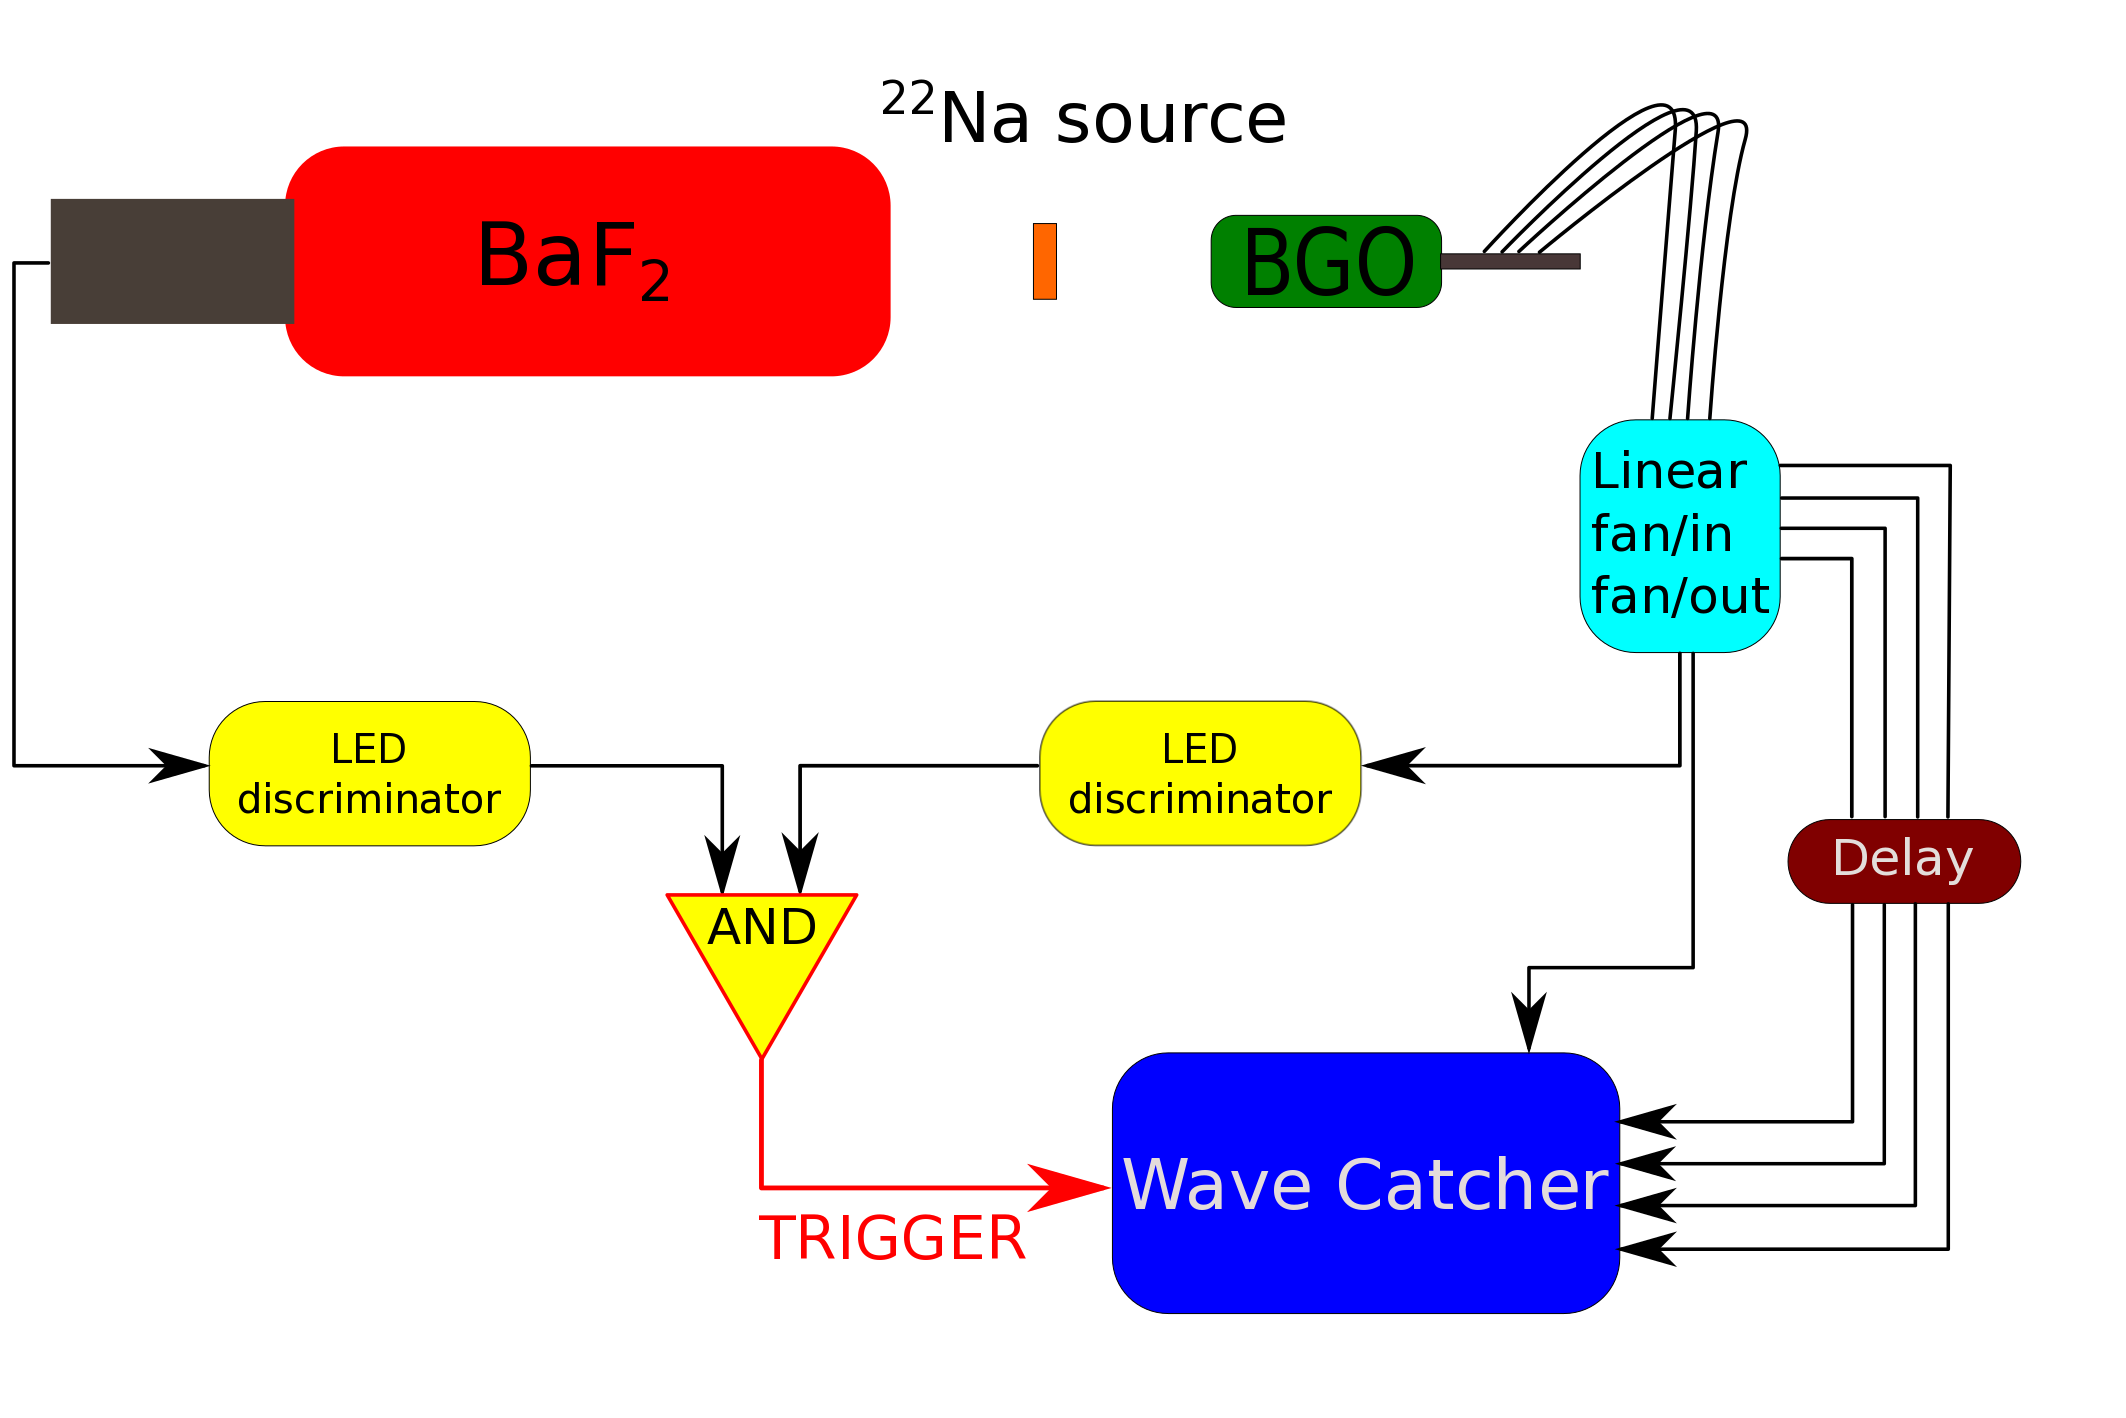
\includegraphics[width=1\textwidth]{03_GraphicFiles/chapter3_CLaRySproto/Absorber/images/timing_meas_scheme.png}
\caption{Scheme of the time response characterization test-bench.}
\label{chap3::fig::BGOtime_meas_scheme}
\end{subfigure}
\caption{Details about the \gls{bgo} block time response characterization.}
\label{chap3::fig::BGO_timingDaq}
\end{figure}

\subsubsection{Space and energy calibration and characterization}\label{chap3::subsubsec::absSpaceEnMethod}

The space and energy calibration process is mainly divided into three stages:
\begin{itemize}
\item \underline{Channel equalization ($^{22}$Na)}: the block is irradiated with the $^{22}$Na source and the raw \gls{adc} distributions for the four \glspl{pm} are retrieved. The last falloff in the raw \gls{adc} spectra are taken as reference to equalize the distributions. Four energy calibration factors are extracted and used to the data correction; this correction corresponds to a \gls{pm} gain equalization.

\item \underline{Pixel identification ($^{60}$Co)}: once the calibration factor are extracted thanks to the $^{22}$Na irradiation data, the block is exposed to the $^{60}$Co source. The collected data are analyzed as in the previous step and calibrated according to the already calculated correction factors. The energy spectrum, the mono-dimensional spatial projections and the flood map are produced. The custom algorithm briefly described in the following section~\ref{chap3::subsubsec::absPixel_ID_algo} has been developed to identify the pseudo-pixel positions on the flood map. It is applied to the $^{60}$Co irradiation data and the pseudo-pixel position map is stored. 

\item \underline{Pixel energy calibration}: the $^{22}$Na irradiation data are re-analyzed in this last calibration step in order to assign each interaction to a single pseudo-pixel according to the pixel position map obtained with the $^{60}$Co data. The energy spectrum of each pixel can be then produced and the two identified peaks (corresponding to the two photon energies emitted by the $^{22}$Na source - 511~keV and 1275~keV) can be used to equalize the pseudo-pixel response. The sum of all the pixels spectra produces the block energy spectrum. At this stage, the \gls{adc} channel values are calibrated to obtain the absorbed energy values in keV.     
\end{itemize}

It is worth to notice that the $^{60}$Co irradiation is useful for the pixel identification given the high energy and narrow energy range of the emitted photons. The equalization factors obtained with the $^{22}$Na source irradiation have been verified to be consistent with the $^{60}$Co irradiation data, as expected. In addition to this, the pixel position map obtained with the $^{60}$Co irradiation data has been verified to fit with the $^{22}$Na data, which presents larger distributions around the pseudo-pixel center. The whole method results to be robust.

\subsubsection{Qualitative test of spatial reconstruction accuracy}\label{chap3::subsubsec::test_spatial_scan}

Specific acquisitions have been devoted to the test of the block spatial accuracy potential. The detector is expected to be able to locate the collected interaction on the pseudo-pixel grid, but the possible sub-pixel accuracy can be tested with a collimated source scan of the block surface. The $^{60}$Co source has been employed for this purpose, with the linear aperture. The block has been placed on a moving table with no distance between its entrance surface and the collimator aperture. The whole surface have been irradiated with horizontal and vertical movements of 1~mm and 2~mm per step. The collected data have been calibrated with the factors obtained with the homogeneous $^{22}$Na irradiation, as explained in the previous section. The results are shown and qualitatively discussed in section~\ref{chap3::subsubsec::absBlockSpatialAcc}. 

PUT ALSO POINT-LIKE SCAN ????

\subsubsection{Pixel identification and energy calibration algorithm}\label{chap3::subsubsec::absPixel_ID_algo}
An automatic algorithm has been developed to identify the block pseudo-pixel positions starting from the calibrated and reconstructed data. Starting from the integrated mono-dimensional spatial projections along the two axes obtained from the calibrated flood map, the distributions peaks and valleys are derived with the ROOT methods included in the TSpectrum class and simple analytic calculations. With the resulting valley positions, a grid is created on the flood map with a pixel-by-pixel center of gravity calculation: each grid portion should contain a single peak, corresponding to the center of the related pseudo-pixel. Spatial reconstruction artifacts can determine a non complete identification of the 64 pseudo-pixels, and the algorithm is able to check for errors of this kind. In case the identified valleys are less then seven on each axis (corresponding to a 8$\times$8 pseudo-pixel array), the projection of each identified region (rows and columns) on the two axis is created and re-analyzed looking for peaks and valleys as before. The values obtained for the rows and columns are compared and a new, fine-tuned grid is produced. This process can be iterated a given number of times if a complete grid is not obtained. Once the pseudo-pixels grid is fixed, the maximum of each region is automatically identified and its position defines the pseudo-pixel center relative position in the map. The event data are then assigned to the pseudo-pixels with the application of the following process. A new grid composed of the average points on the borders between pixels is created and the reconstructed event position is compared to each point of this map to identify the most likely pseudo-pixel. This is done by calculating the minimal distance between a column and a row average point with respect to the reconstructed event and then calculating two external products, between the vector connecting the reconstructed point and closest column (row) average point and the vector connecting this average point to the previous or next one on the same column (row). The sign of the products defines the column (row) where to assign the interaction. 
Knowing the relative position of the interaction point with respect to the two minimal distance points on row and column, the correct pseudo-pixel is identified.    
A more simple approach can be based on the research of the minimal distance between the reconstructed event position and the center of the identified pseudo-pixels. This method has been tested and showed some assignment uncertainties due to the position distortions on the pseudo-pixels map. 


\subsubsection{Time response characterization method}\label{chap3::subsubsec::absTimeMethod}

The test-bench for the time response characterization has been set as shown in \figurename~\ref{chap3::fig::BGOtime_meas_scheme}. A \gls{baf2} mono-block scintillator, read-out by a single photo-multiplier tube, has been used as reference detector. Its excellent time resolution makes it suitable for relative timing measurements in comparison to the \gls{bgo} blocks. The reference scintillator and the \gls{bgo} block under test have been set at arbitrary distances from the $^{22}$Na source with the aim of detecting in coincidence the two 511~keV back-to-back photons resulting from the positron annihilation. The four raw signals coming out from the \gls{bgo} block are summed with a \gls{nim} linear fan-in/fan-out module, and the resulting signal is sent to a leading edge discriminator and converted to a logic signal according to a fixed threshold. The single signal emerging from the reference detector passes through a selected threshold and is converted to digital. The two digital signals, 100~ns width, are then sent to a logic coincidence module to create the trigger input for the WaveCatcher acquisition system described in section~\ref{chap3::subsec::absBGOchar}. The four \gls{bgo} output raw signals, the reference scintillator raw output signal and the sum of the four raw \gls{bgo} signals are sent to the WaveCatcher for digitization.\\
For each coincidence event, the six collected signals are analyzed with focus on the signal rising edge. The time corresponding to the amplitude maximum and to 20\%, 30\%, 50\% and 80\% of the maximum is retrieved for constant fraction discrimination tests. In addition to this, a fixed threshold is used for fixed value discrimination.\\
Different comparison methods have been tested in order to identify the more robust one for the definition of the time resolution of the blocks. The chaotic structure of the single \gls{bgo} raw signals leads to very variable results depending on the defined threshold, and the more stable results are given by the comparison of the sum of the four \gls{bgo} signals and the reference scintillator with the arrival time identified by a fixed tuned threshold. With this method, the arrival time of each signal can be defined and the time difference distribution of the two signals can be produced.\\
The same analysis has been applied to a data set obtained with two identical \gls{baf2} detectors exposed to the $^{22}$Na source in coincidence. This data set allowed for the definition of the reference scintillator time resolution.\\
The resulting \gls{bgo} time resolution is defined as the \gls{fwhm} of arrival time difference distribution between \gls{bgo} block and reference scintillator, with the subtraction of the reference scintillator contribution via uncertainties composition calculation.\\


\subsubsection{Results: \gls{pm} gain equalization}\label{chap3::subsubsec::absPMgainCal}
Figures~\ref{chap3::fig::absPM_amp},~\ref{chap3::fig::absXYprofiles},~\ref{chap3::fig::absADCspectrum},~\ref{chap3::fig::absFloodMap} show the effect of the \gls{pm} gain equalization on the data collected with the reference \gls{bgo} block irradiated with the $^{22}$Na source.
Figures~\ref{chap3::fig::absPM_rawProfiles} and~\ref{chap3::fig::absPM_calProfiles} show the raw and equalized \gls{adc} profiles of the four read-out photo-multipliers (the peaks above 3000 \gls{adc} counts in \figurename~\ref{chap3::fig::absPM_rawProfiles} correspond to the saturation of the \gls{nim} linear fan-in/fan-out module used to handle the data read-out; these values are rejected during the equalization stage).
Figures~\ref{chap3::fig::abssingleAxisRawProfile} and~\ref{chap3::fig::abssingleAxisCalProfile} show the projection on the two axes of the position of interaction reconstructed via Anger logic, before (left) and after (right) the \gls{pm} gain equalization.
Figures~\ref{chap3::fig::absRaw_Espectrum} and~\ref{chap3::fig::absCal_Espectrum} show the \gls{adc} event spectrum, obtained by the sum of the \gls{adc} values of the four \glspl{pm}, before (left) and after (right) the \gls{pm} gain equalization.
Figures~\ref{chap3::fig::absraw_floodMap} and~\ref{chap3::fig::abscal_floodMap} show the two dimensional event position map (this will be called \enquote{flood map} in the following) , before (left) and after (right) the \gls{pm} gain equalization; the interaction position is reconstructed via Anger logic (see \figurename~\ref{chap3::fig::BGOblockScheme} for details).

\begin{figure}
\begin{subfigure}[t]{0.5\textwidth}
\centering
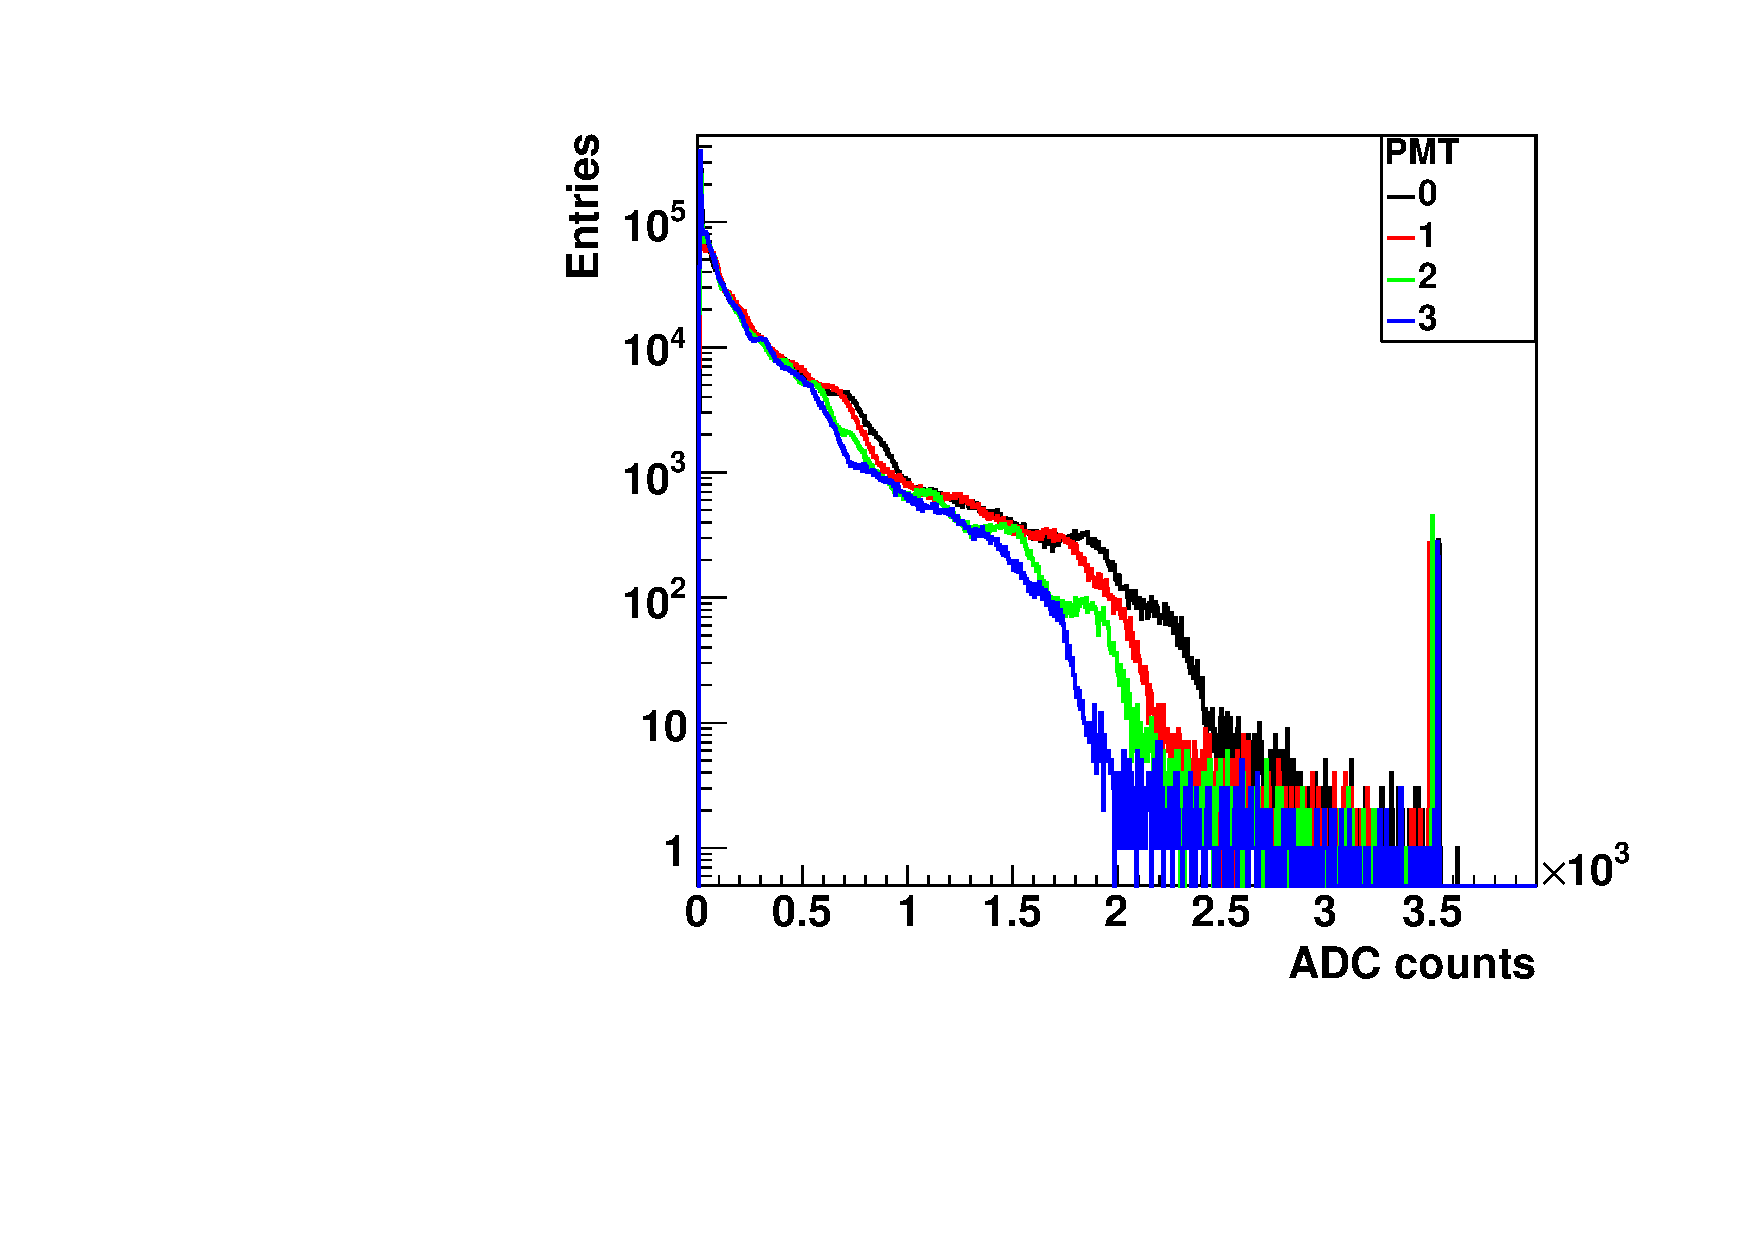
\includegraphics[width=1\textwidth]{03_GraphicFiles/chapter3_CLaRySproto/Absorber/images_charResults_Na22/1_Raw_PMAmp.pdf}
\caption{Before gain equalization.}
\label{chap3::fig::absPM_rawProfiles}
\end{subfigure}
\begin{subfigure}[t]{0.5\textwidth}
\centering
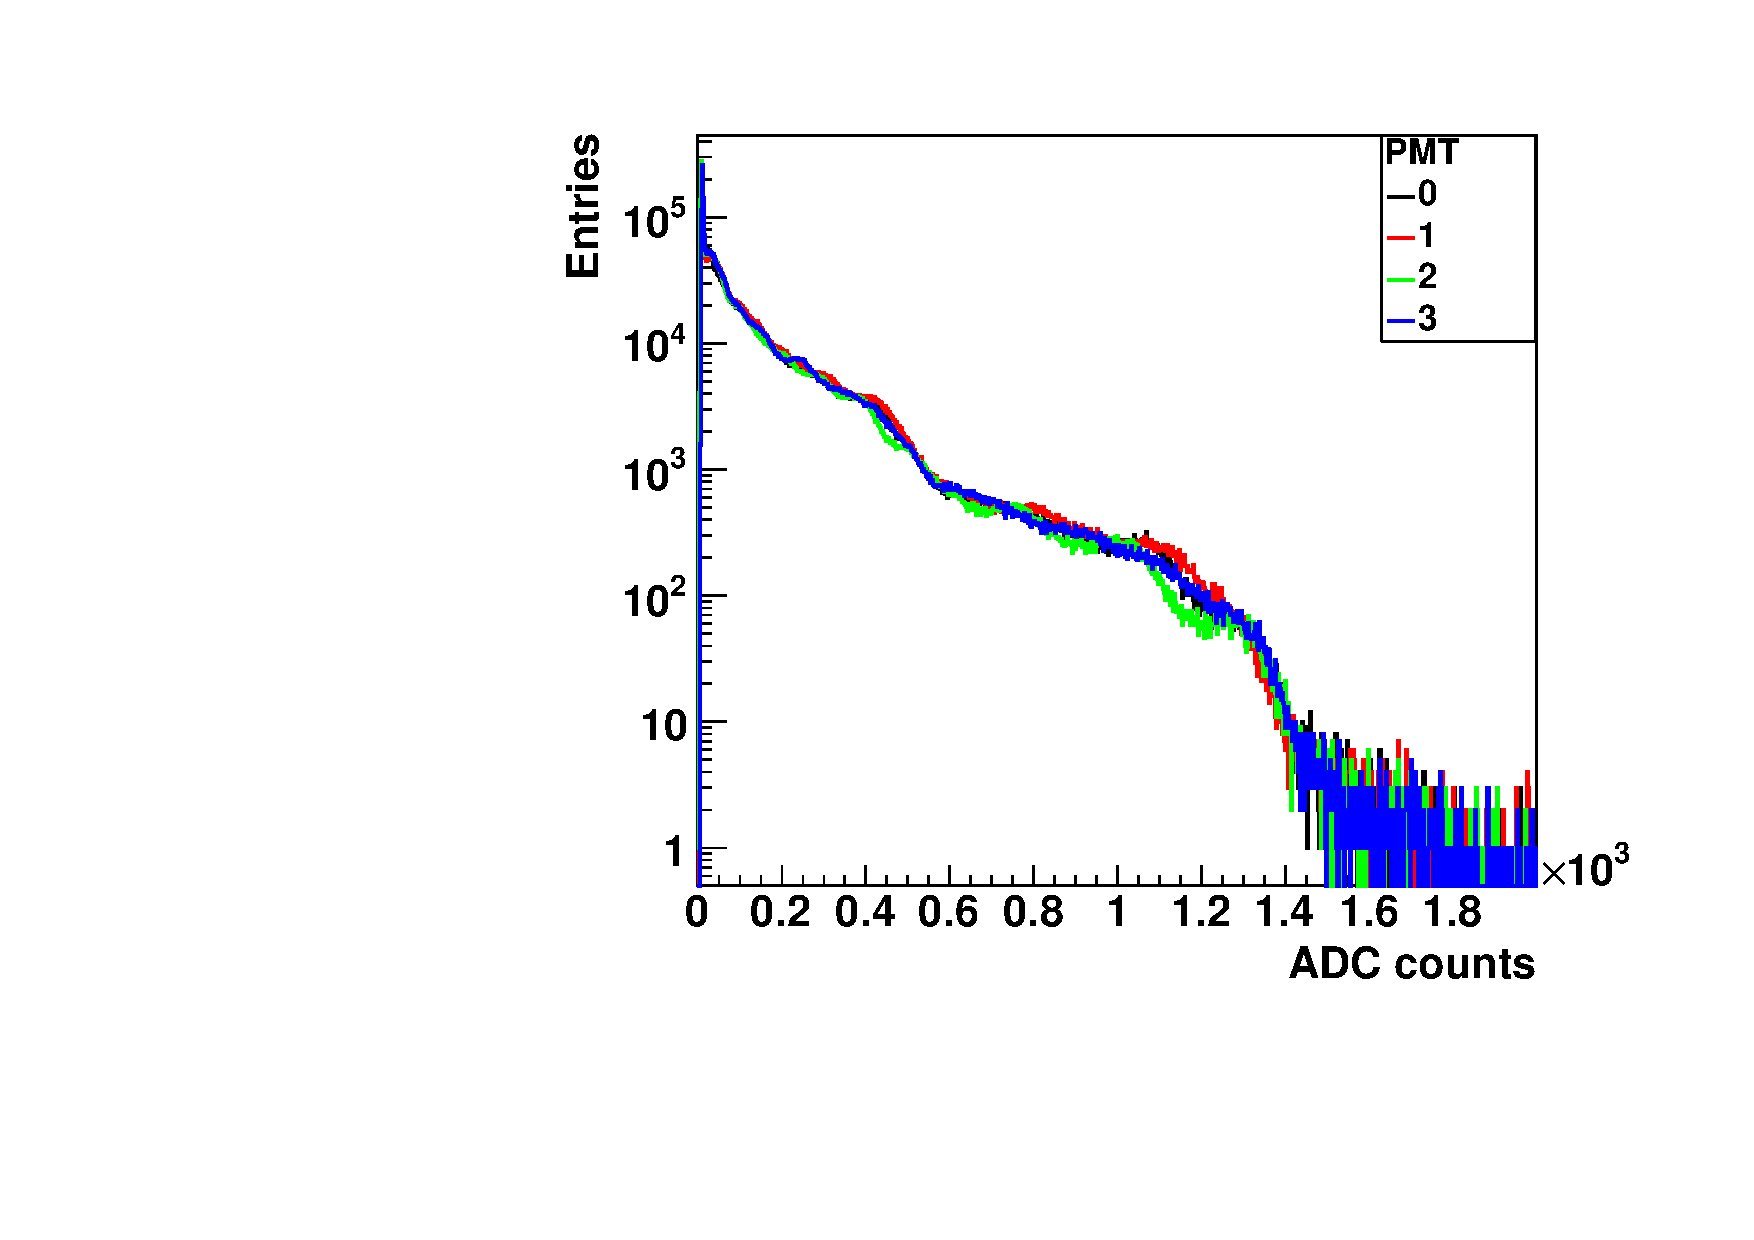
\includegraphics[width=1\textwidth]{03_GraphicFiles/chapter3_CLaRySproto/Absorber/images_charResults_Na22/2_Cal_PMAmp_noSum.pdf}
\caption{After gain equalization.}
\label{chap3::fig::absPM_calProfiles}
\end{subfigure}
\caption{\gls{pm} signal amplitude spectra before (a) and after (b) the \gls{pm} gain equalization.}
\label{chap3::fig::absPM_amp}
\end{figure}

\begin{figure}
\begin{subfigure}[t]{0.5\textwidth}
\centering
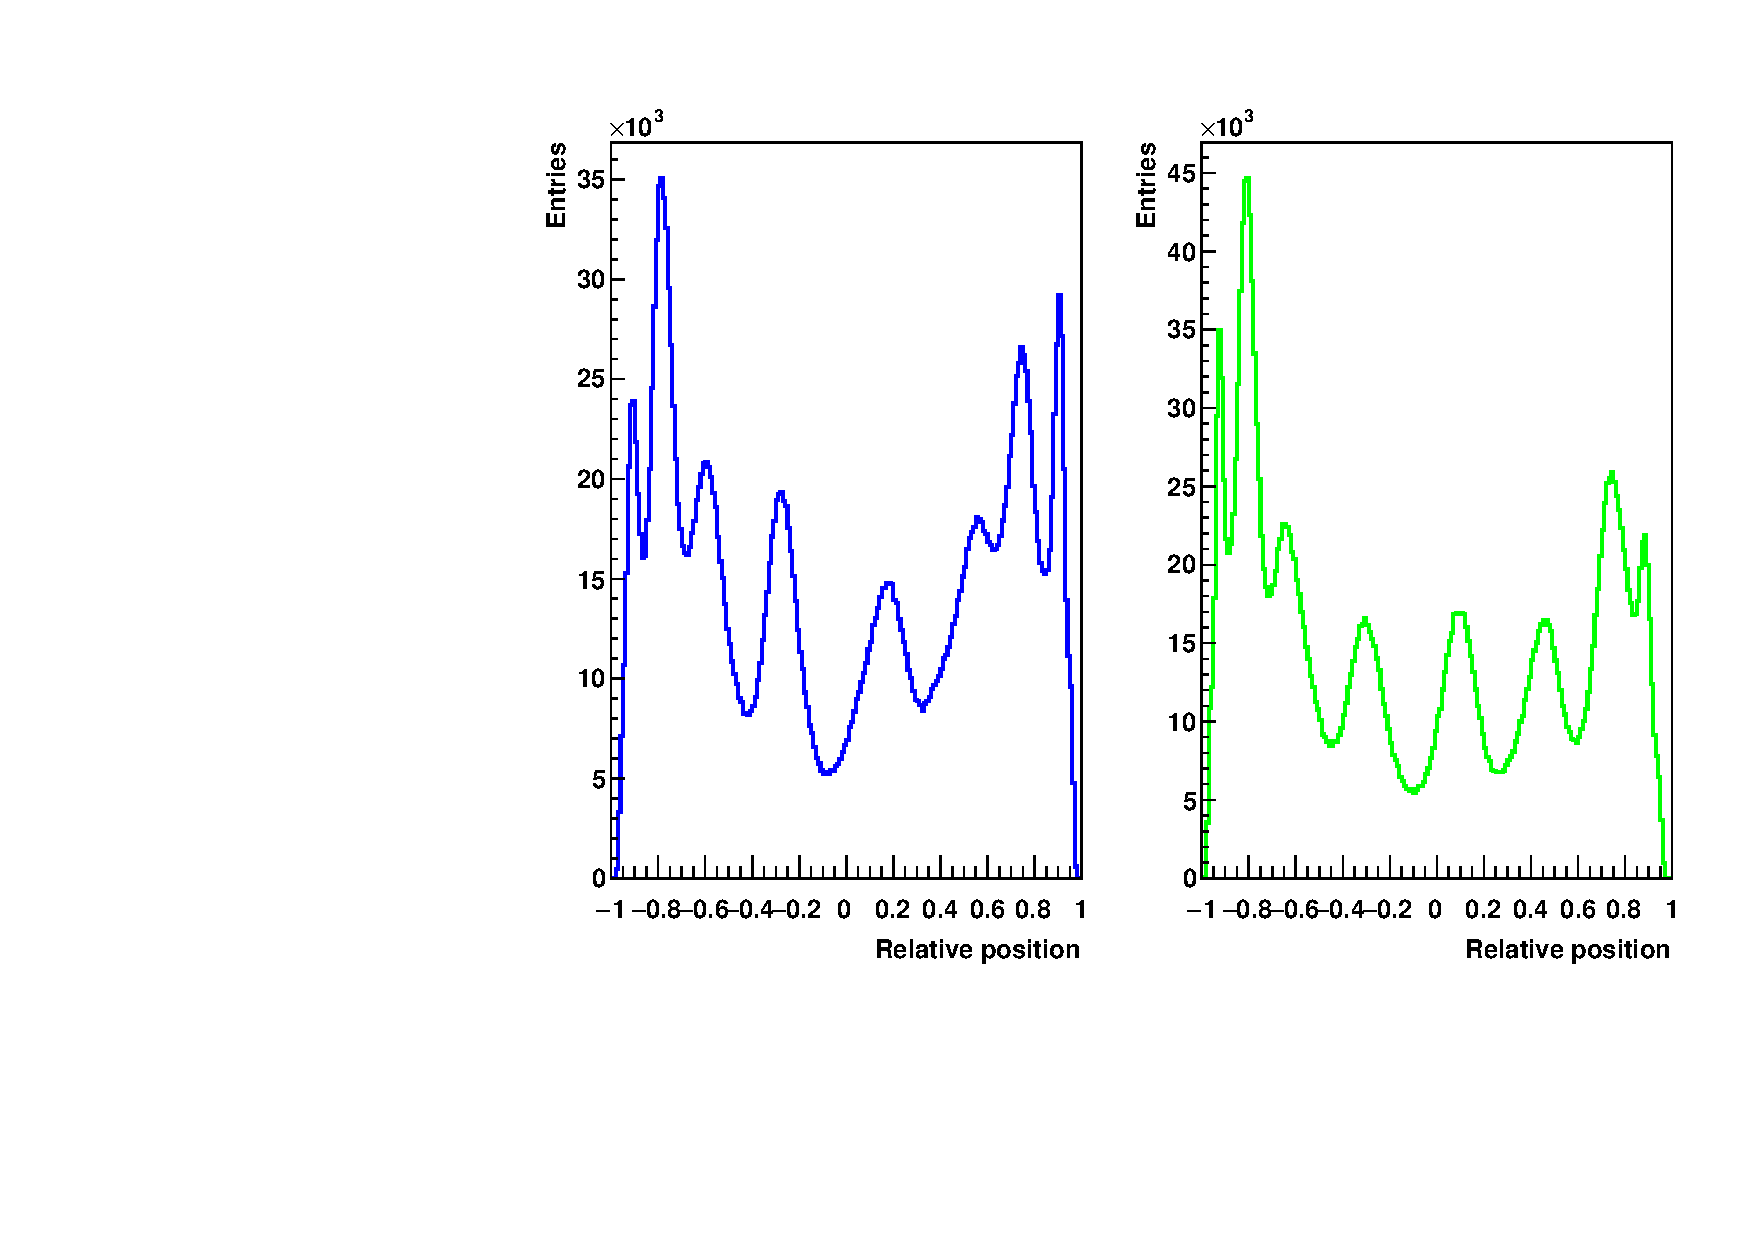
\includegraphics[width=1\textwidth]{03_GraphicFiles/chapter3_CLaRySproto/Absorber/images_charResults_Na22/1_Raw_profileXY_int.pdf}
\caption{Before gain equalization.}
\label{chap3::fig::abssingleAxisRawProfile}
\end{subfigure}
\begin{subfigure}[t]{0.5\textwidth}
\centering
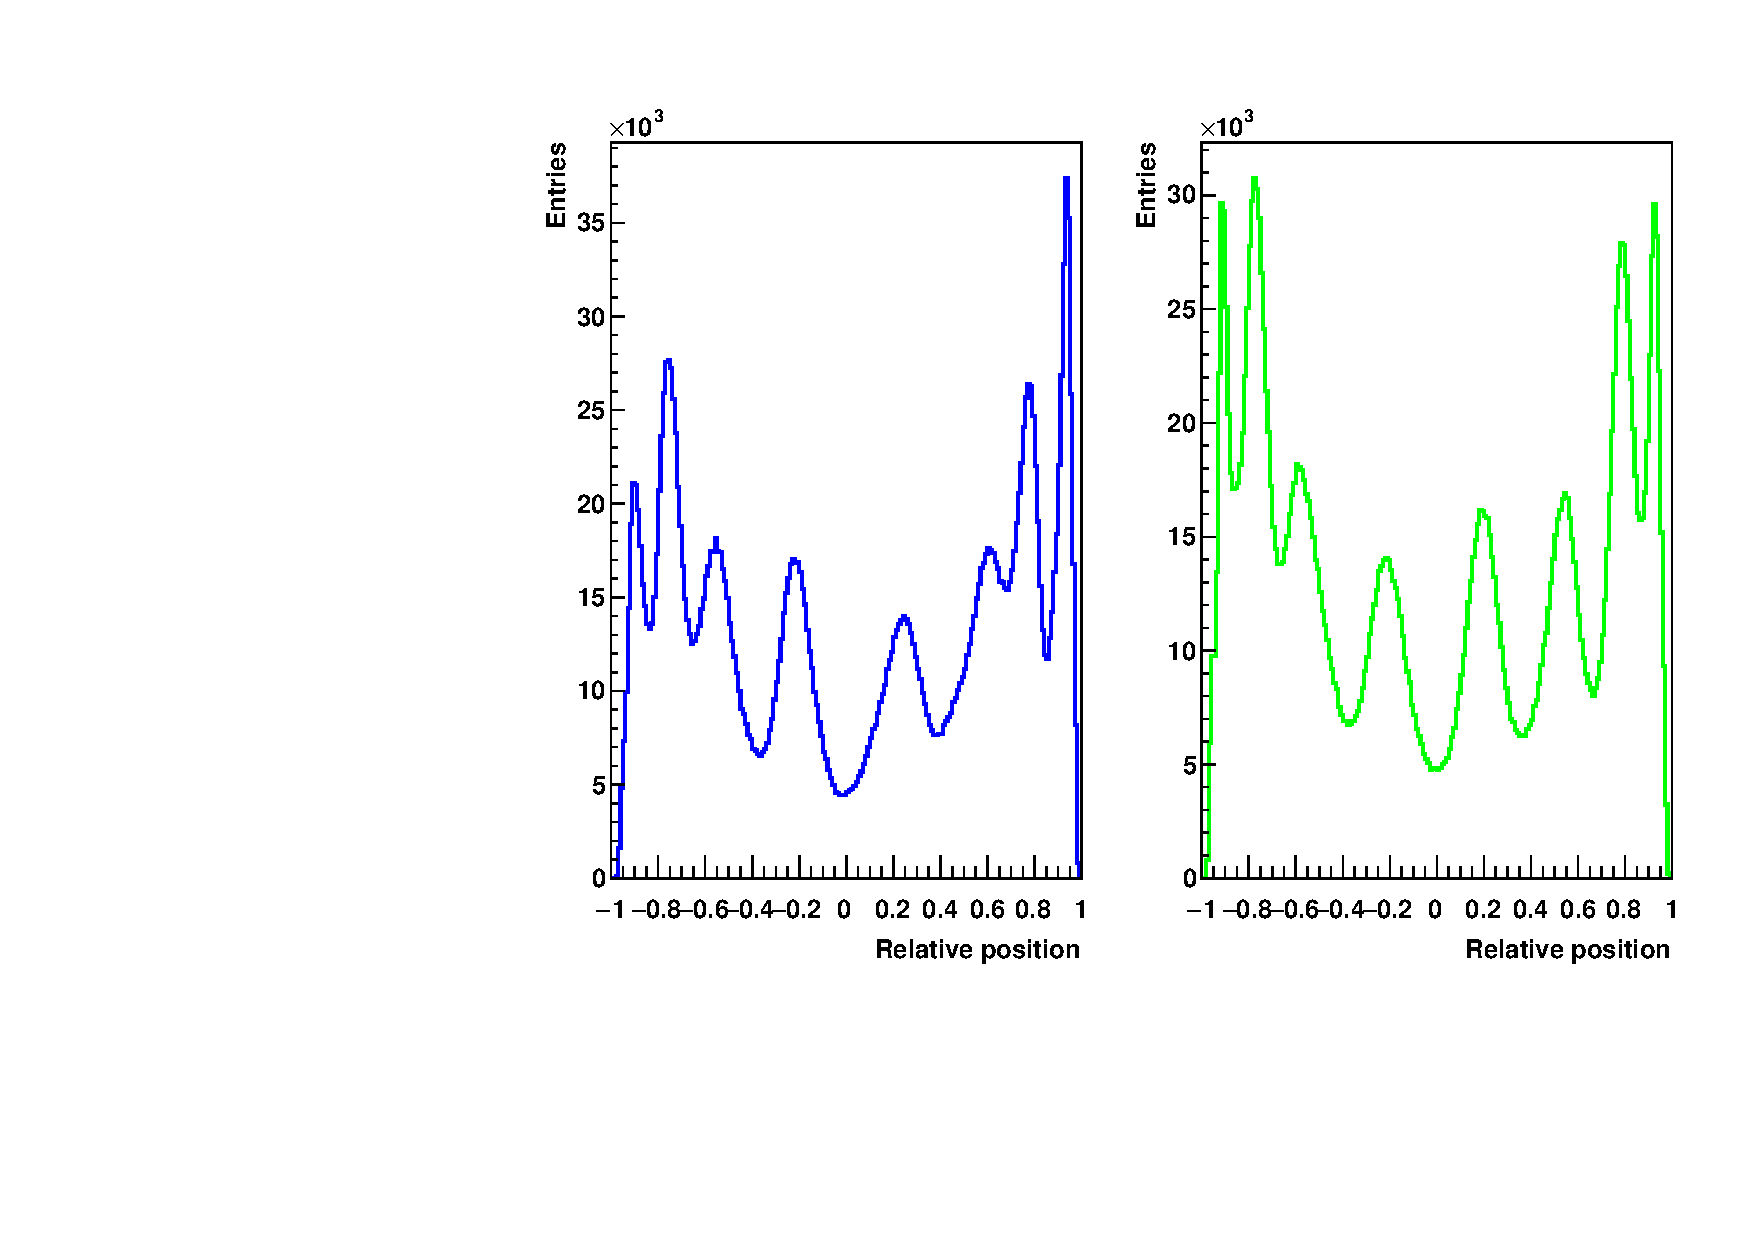
\includegraphics[width=1\textwidth]{03_GraphicFiles/chapter3_CLaRySproto/Absorber/images_charResults_Na22/2_Cal_profileXY_int.pdf}
\caption{After gain equalization.}
\label{chap3::fig::abssingleAxisCalProfile}
\end{subfigure}
\caption{1D integrated position distribution on the two transverse dimensions before (a) and after (b) the \gls{pm} gain equalization. Blue curves: horizontal dimension. Green curves: vertical dimension.}
\label{chap3::fig::absXYprofiles}
\end{figure}

\begin{figure} [!h]
\begin{subfigure}[t]{0.5\textwidth}
\centering
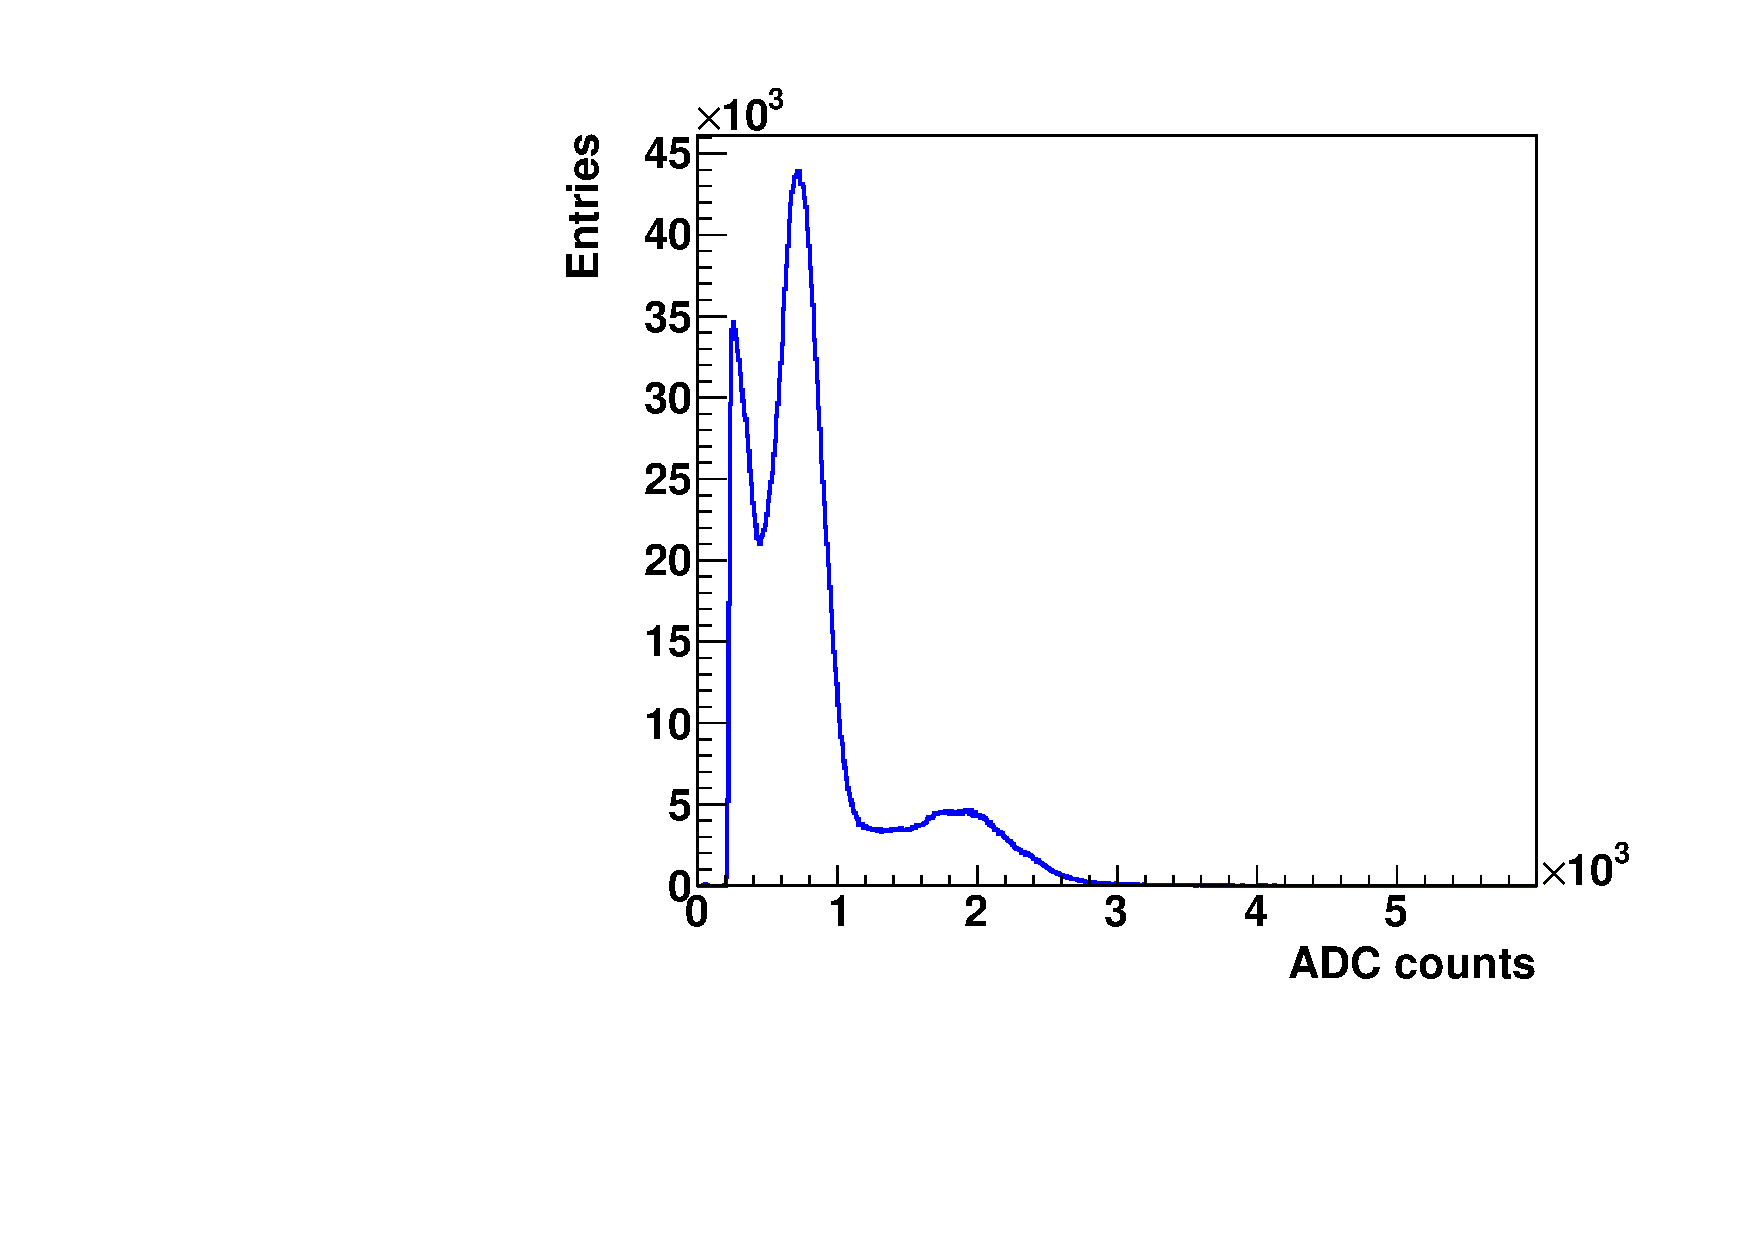
\includegraphics[width=1\textwidth]{03_GraphicFiles/chapter3_CLaRySproto/Absorber/images_charResults_Na22/1_Raw_energy_spectrum.pdf}
\caption{Before gain equalization.}
\label{chap3::fig::absRaw_Espectrum}
\end{subfigure}
\begin{subfigure}[t]{0.5\textwidth}
\centering
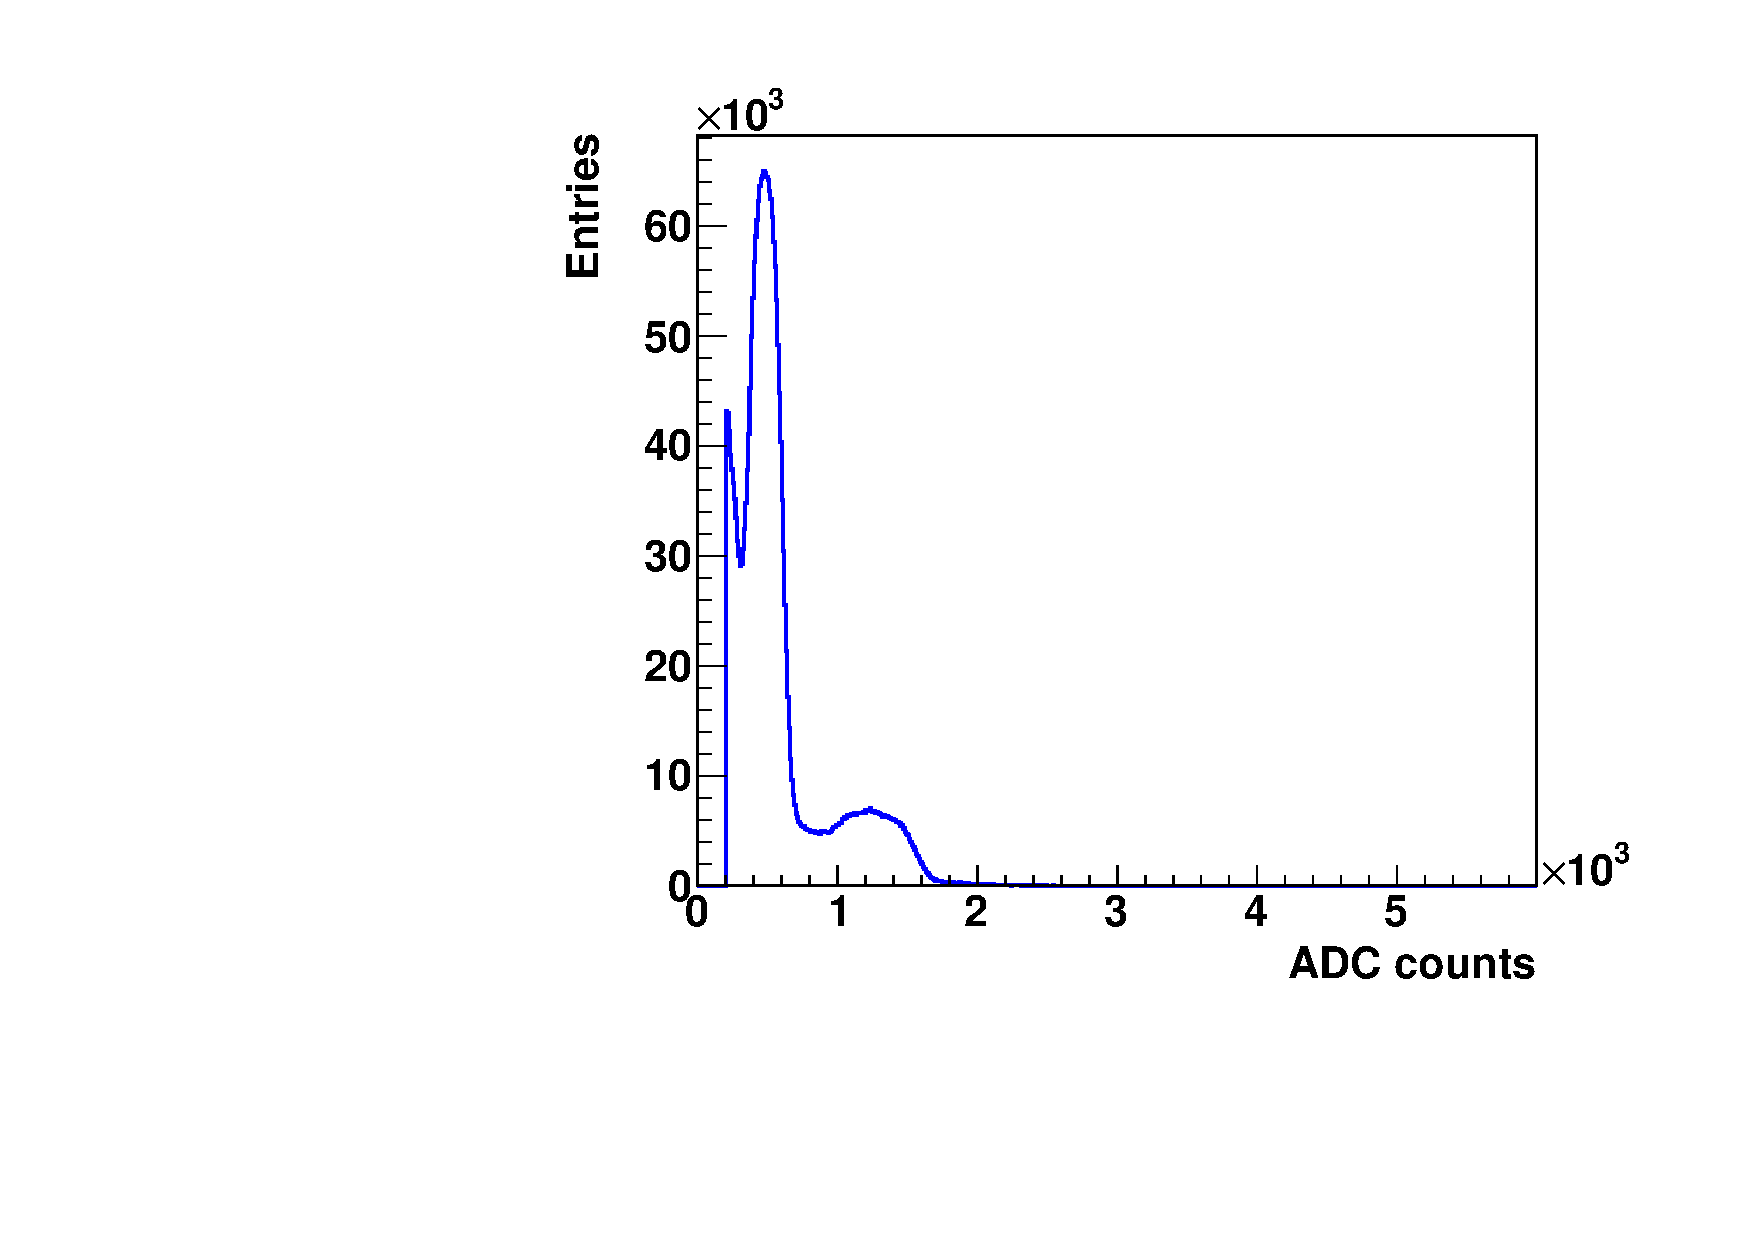
\includegraphics[width=1\textwidth]{03_GraphicFiles/chapter3_CLaRySproto/Absorber/images_charResults_Na22/2_Cal_energy_spectrum.pdf}
\caption{After gain equalization.}
\label{chap3::fig::absCal_Espectrum}
\end{subfigure}
\caption{Block energy spectrum before (a) and after (b) the \gls{pm} gain equalization.}
\label{chap3::fig::absADCspectrum}
\end{figure}

\begin{figure} [!h]
\begin{subfigure}[t]{0.5\textwidth}
\centering
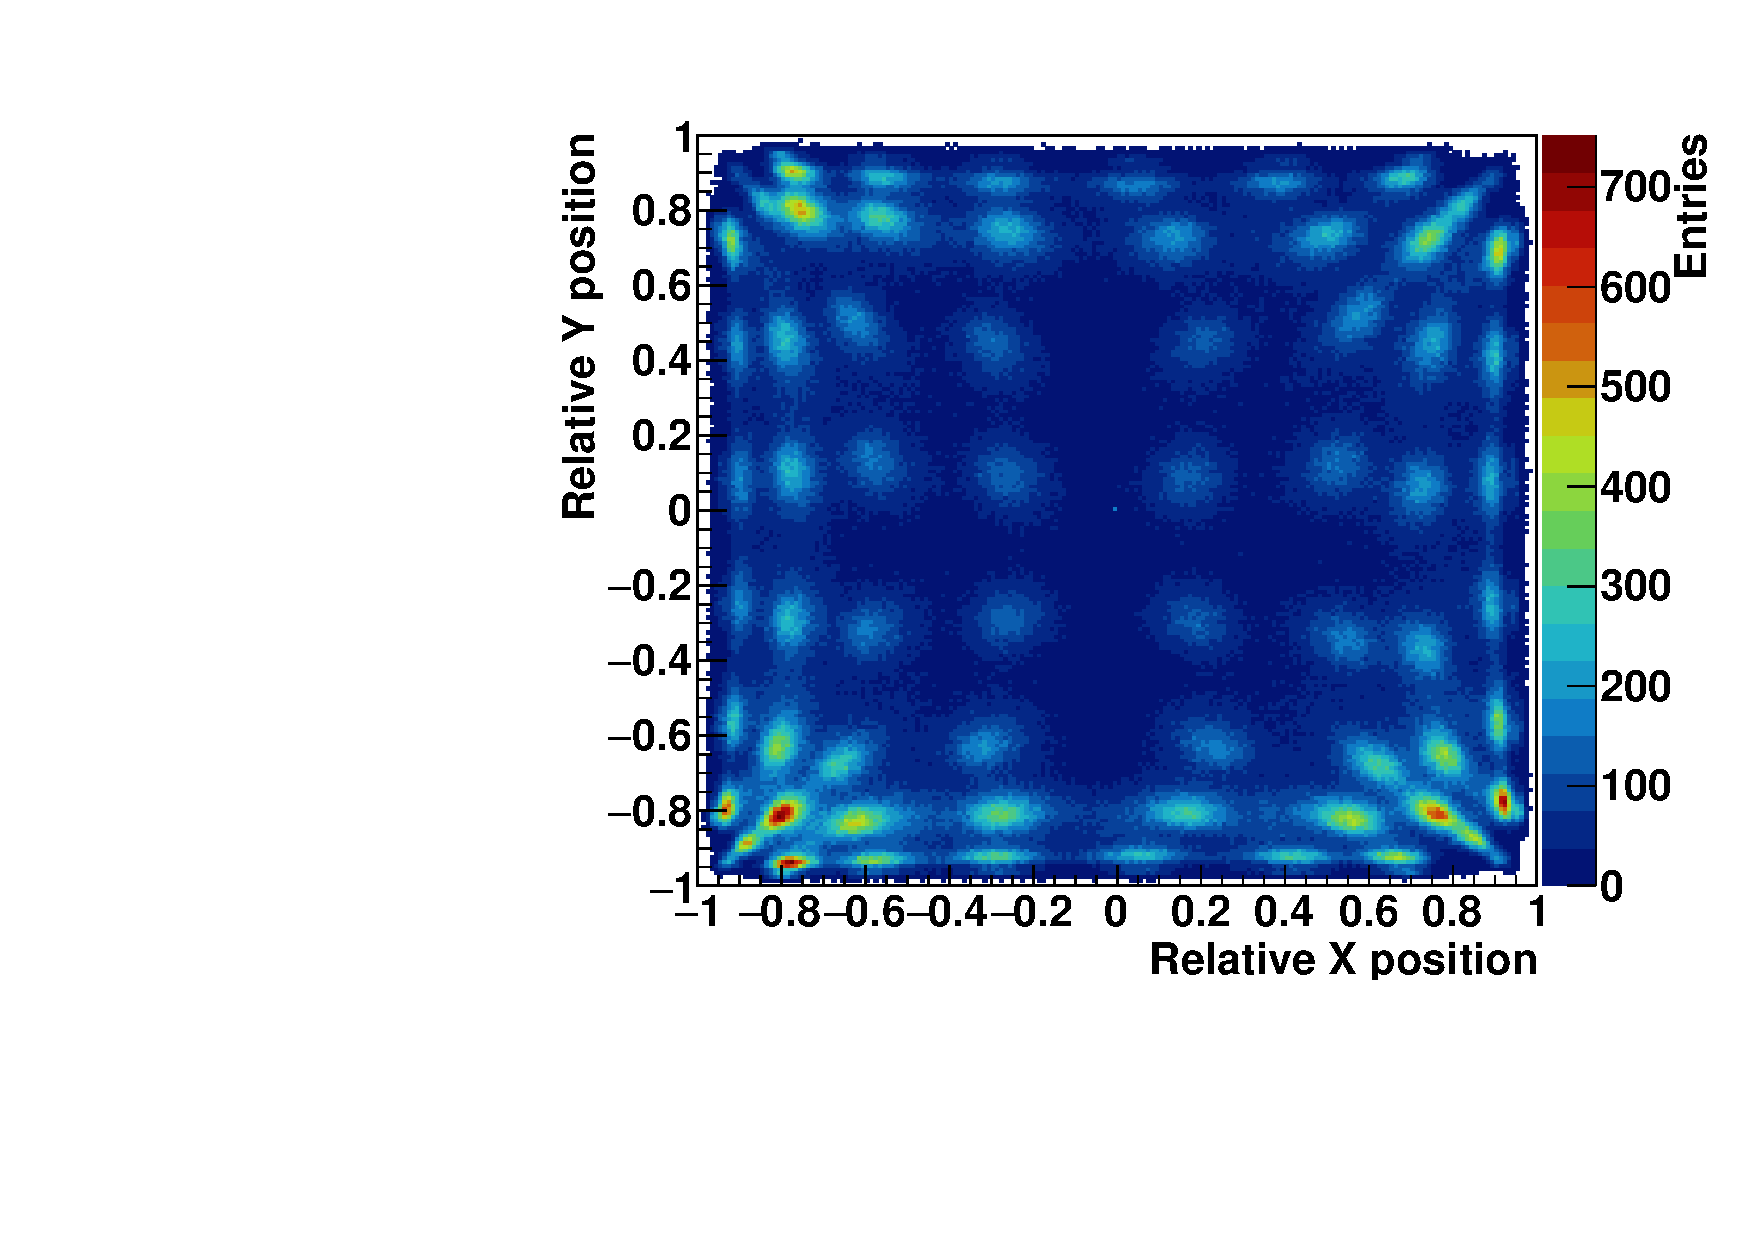
\includegraphics[width=1\textwidth]{03_GraphicFiles/chapter3_CLaRySproto/Absorber/images_charResults_Na22/1_Raw_FLOODMAP.pdf}
\caption{Before gain equalization.}
\label{chap3::fig::absraw_floodMap}
\end{subfigure}
\begin{subfigure}[t]{0.5\textwidth}
\centering
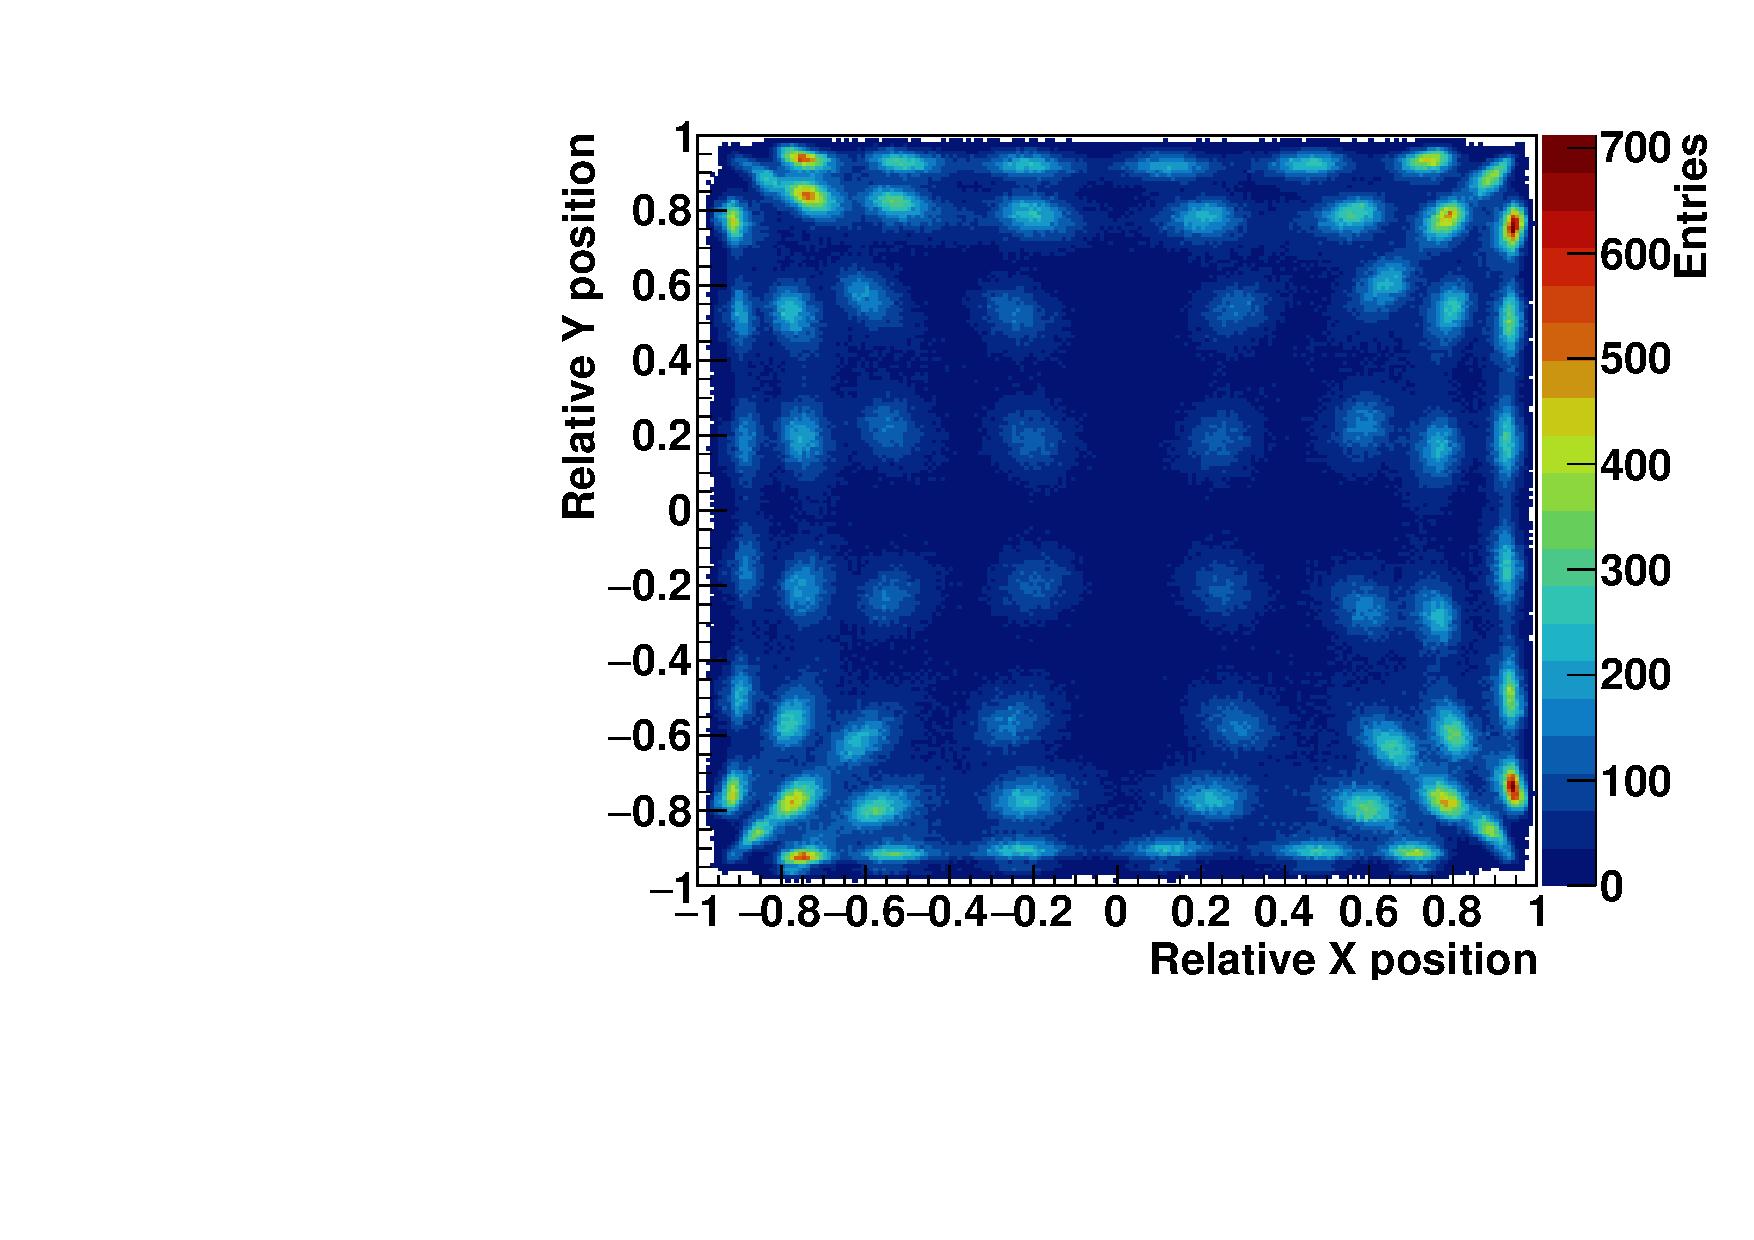
\includegraphics[width=1\textwidth]{03_GraphicFiles/chapter3_CLaRySproto/Absorber/images_charResults_Na22/2_Cal_FLOODMAP.pdf}
\caption{After gain equalization.}
\label{chap3::fig::abscal_floodMap}
\end{subfigure}
\caption{2D reconstructed position map before (a) and after (b) the \gls{pm} gain equalization.}
\label{chap3::fig::absFloodMap}
\end{figure}

As shown by Figures~\ref{chap3::fig::absPM_amp} to~\ref{chap3::fig::absFloodMap}, the \gls{pm} gain equalization performed in this first calibration step is mandatory to optimize the spatial and energy response of the tested block. \figurename~\ref{chap3::fig::abssingleAxisCalProfile} highlights the better definition of the pseudo-pixels ensured by the gain equalization: the peak-to-valley ratio is increased, in particular for the most external pixels. The spatial response improvement is also reflected in a better energy response, as shown in \figurename~\ref{chap3::fig::absCal_Espectrum}, where the two energy peaks of the $^{22}$Na source are more narrow with respect to the ones obtained with the raw data. The obtained energy response is still not satisfactory, and the next steps of the calibration process are dedicated to the improvement of this result. The flood map in \figurename~\ref{chap3::fig::abscal_floodMap} shows how the gain equalization and the offset tuning allow to arrange the position map over the whole block surface; the borders are better defined and the pseudo-pixels on the block limits (especially on the corner) are better separated. 


\subsubsection{Results: block spatial accuracy}\label{chap3::subsubsec::absBlockSpatialAcc}

\begin{figure}
\begin{subfigure}[t]{0.5\textwidth}
\centering
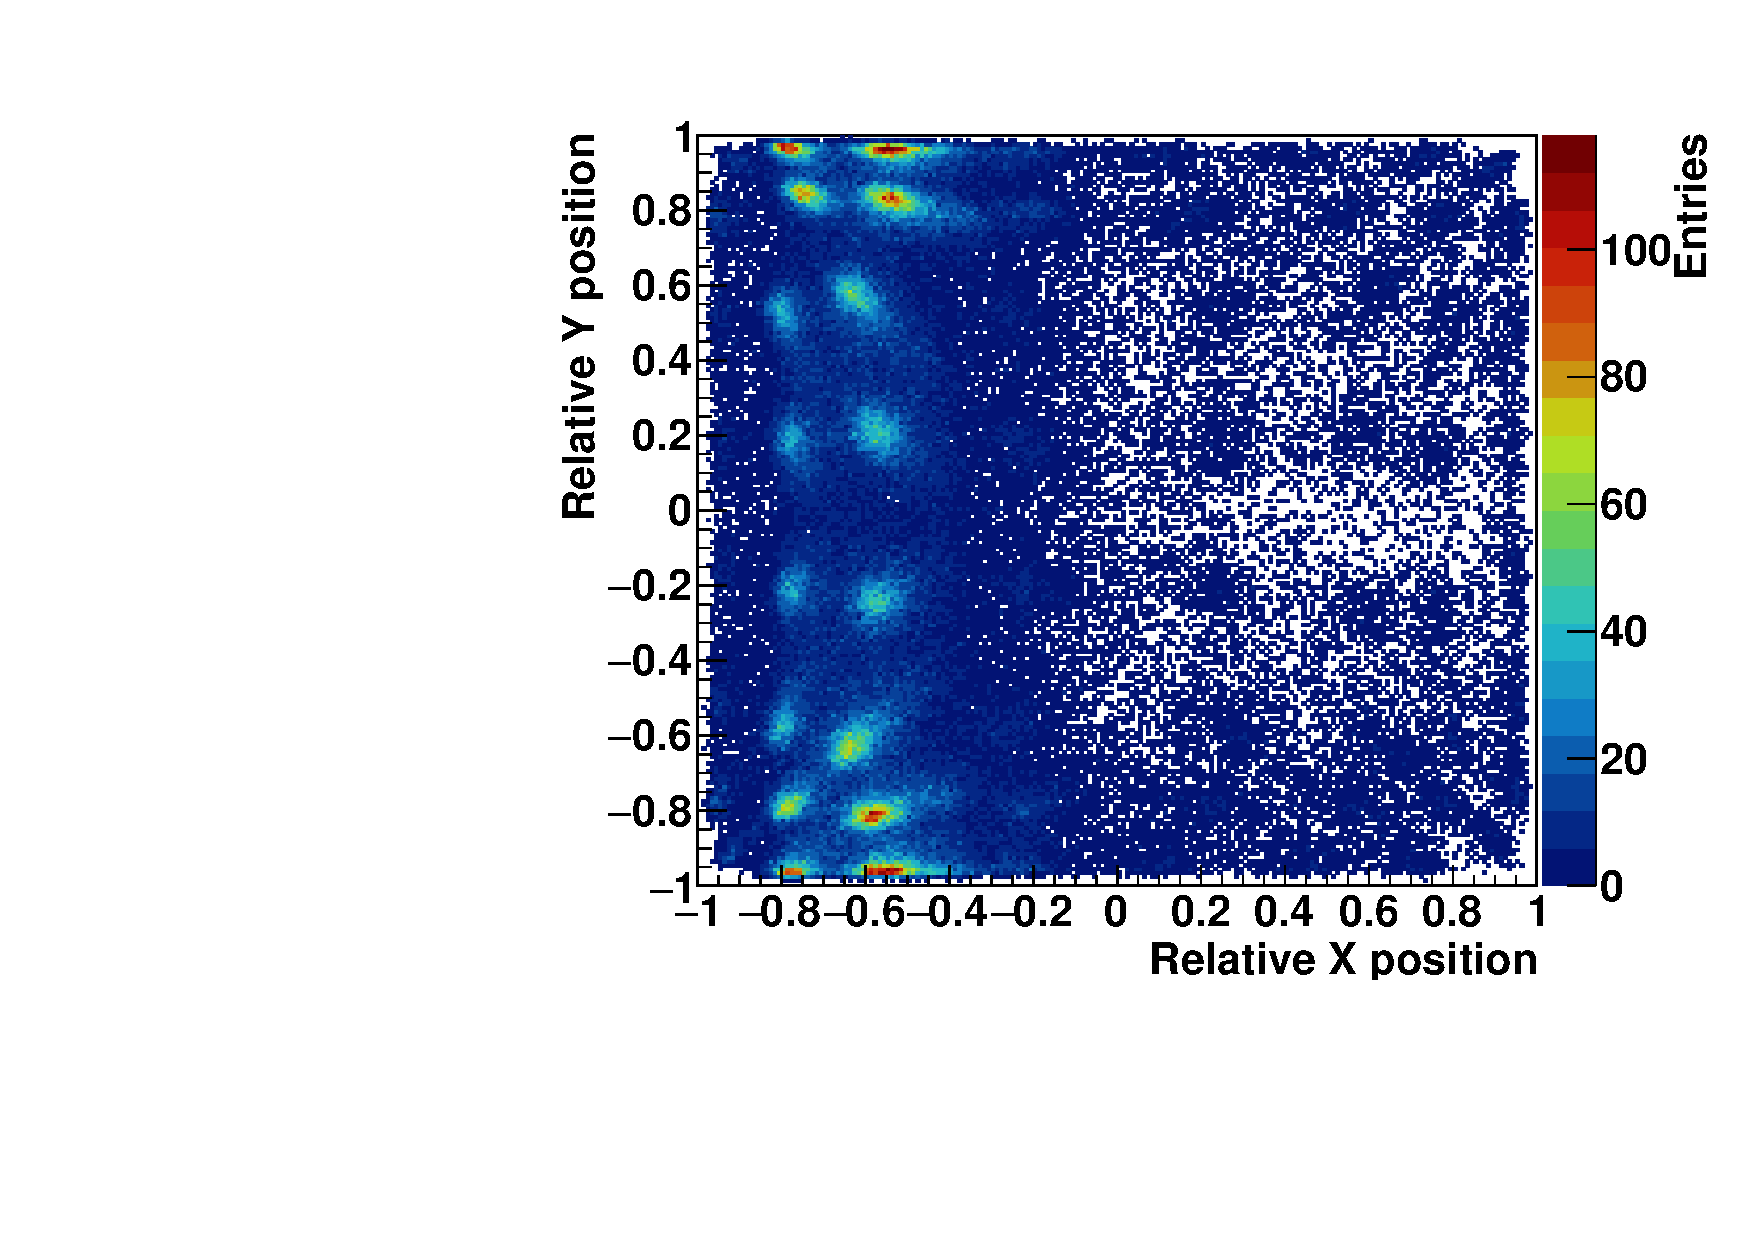
\includegraphics[width=\textwidth]{03_GraphicFiles/chapter3_CLaRySproto/Absorber/images_scan/line_2mm/run8_floodMap.pdf}
\caption{Aperture center relative X position: \\ -0.675}
\label{chap3::fig::scan_map1}
\end{subfigure}
\begin{subfigure}[t]{0.5\textwidth}
\centering
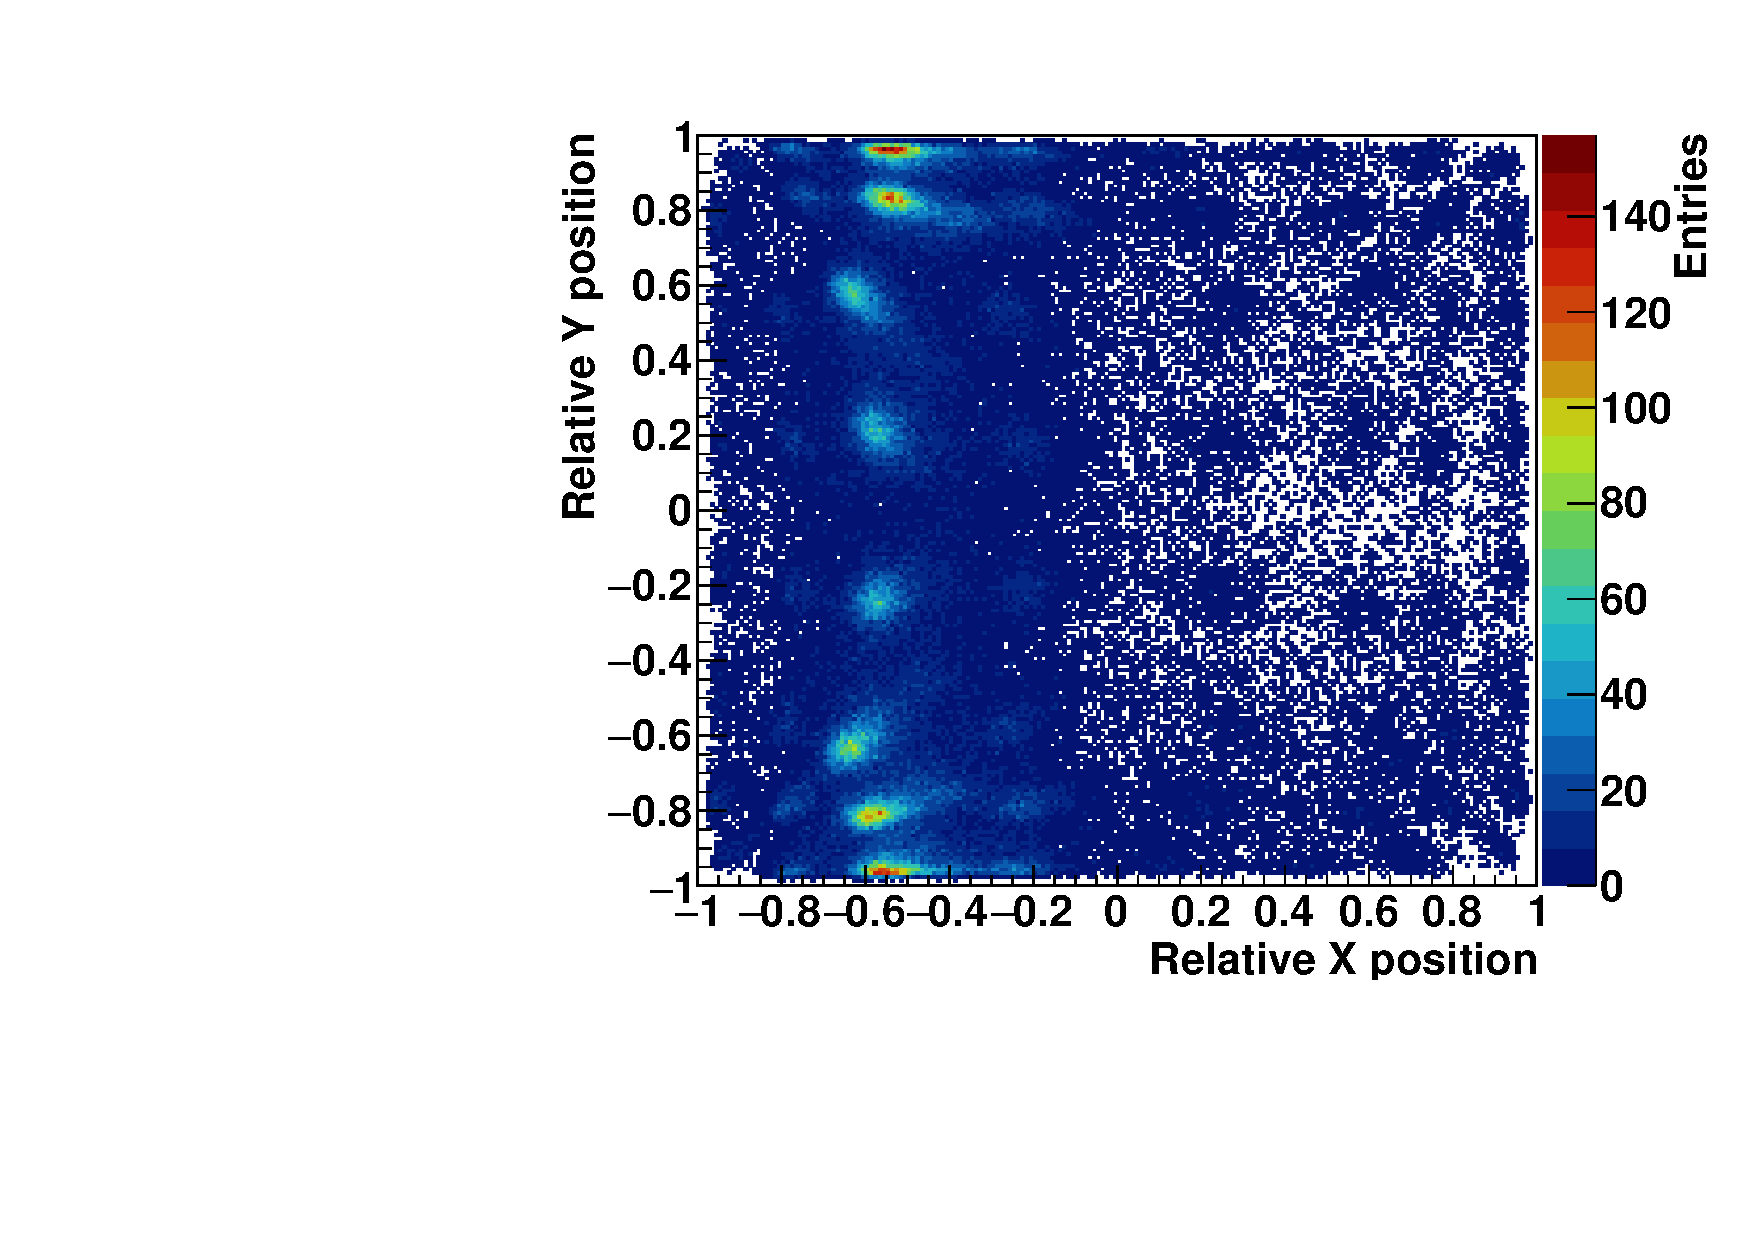
\includegraphics[width=\textwidth]{03_GraphicFiles/chapter3_CLaRySproto/Absorber/images_scan/line_2mm/run9_floodMap.pdf}
\caption{Aperture center relative X position: \\ -0.560}
\label{chap3::fig::scan_map2}
\end{subfigure}\newline
\begin{subfigure}[t]{0.5\textwidth}
\centering
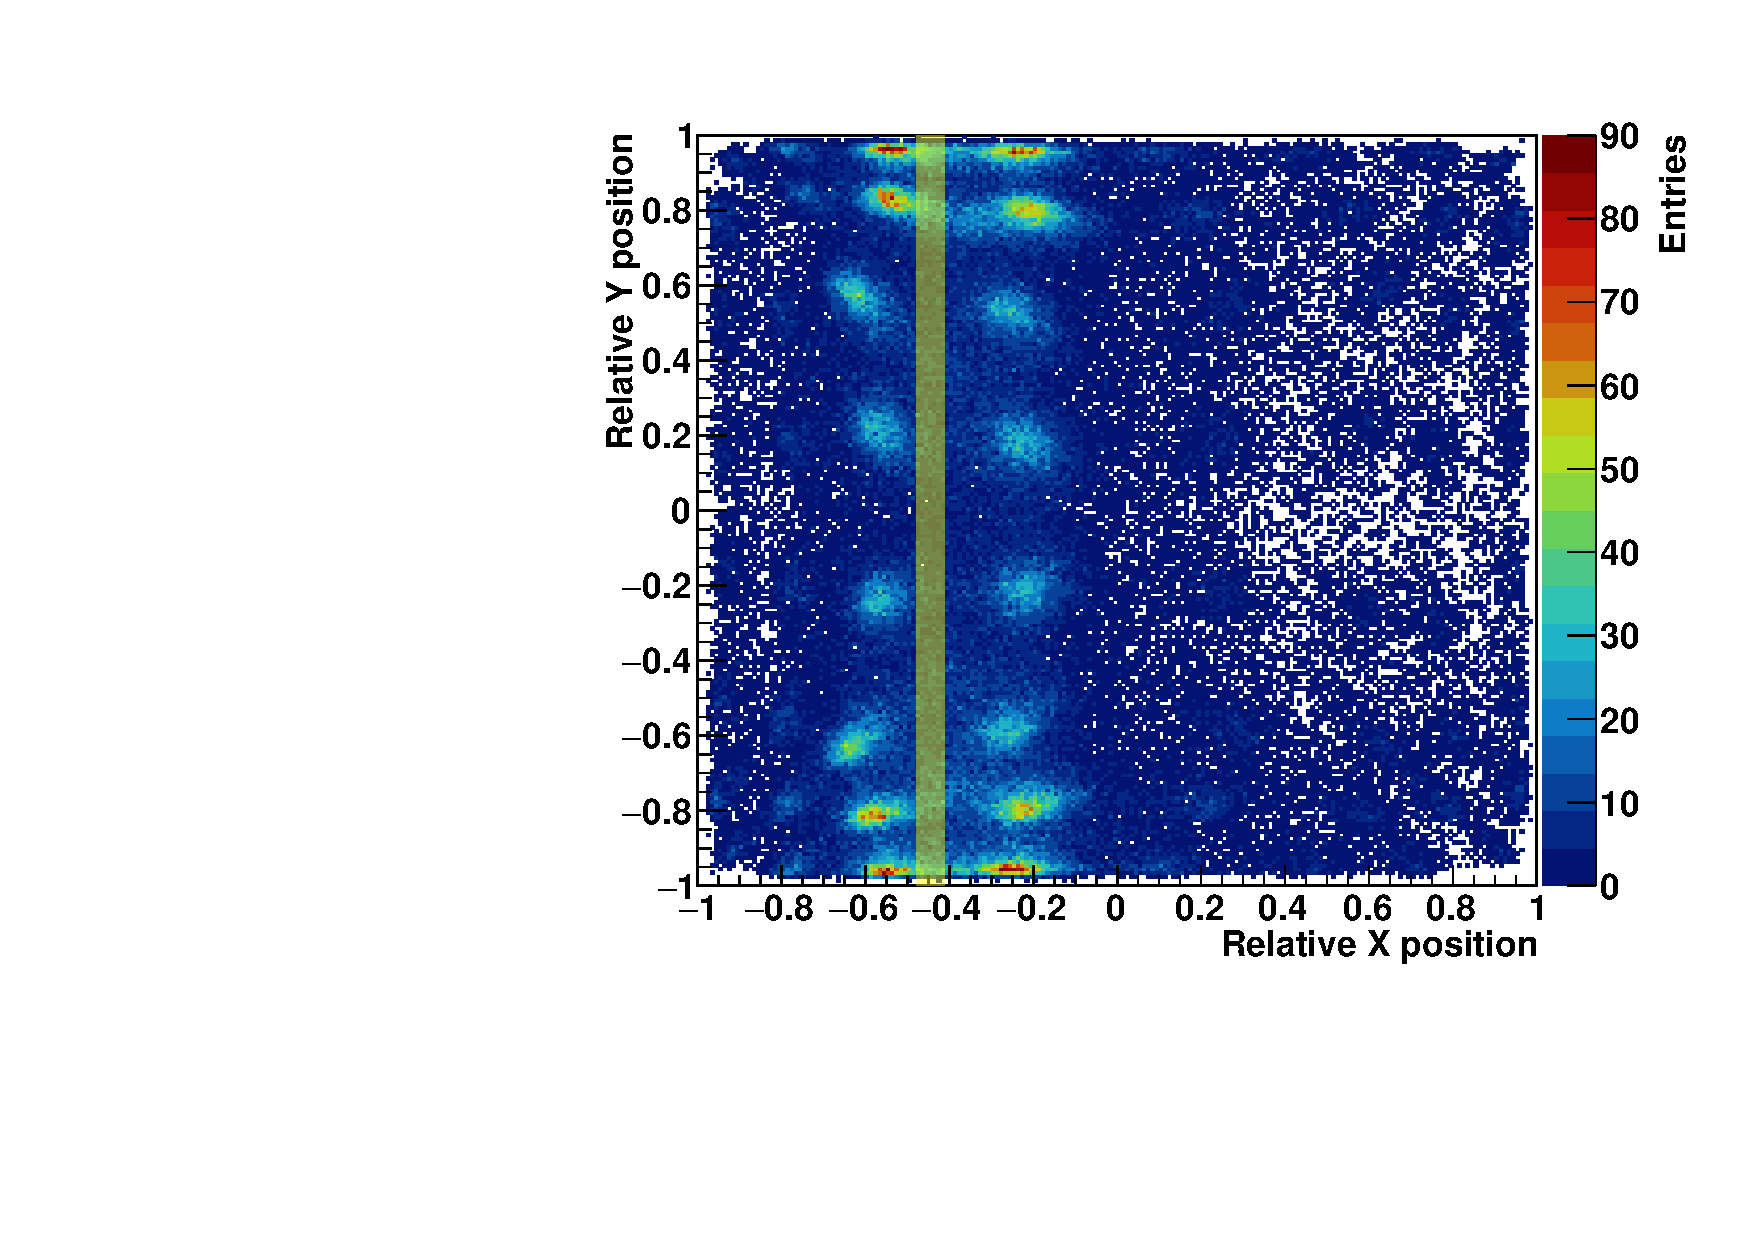
\includegraphics[width=\textwidth]{03_GraphicFiles/chapter3_CLaRySproto/Absorber/images_scan/line_2mm/run10_floodMap.pdf}
\caption{Aperture center relative X position: \\ -0.445}
\label{chap3::fig::scan_map3}
\end{subfigure}
\begin{subfigure}[t]{0.5\textwidth}
\centering
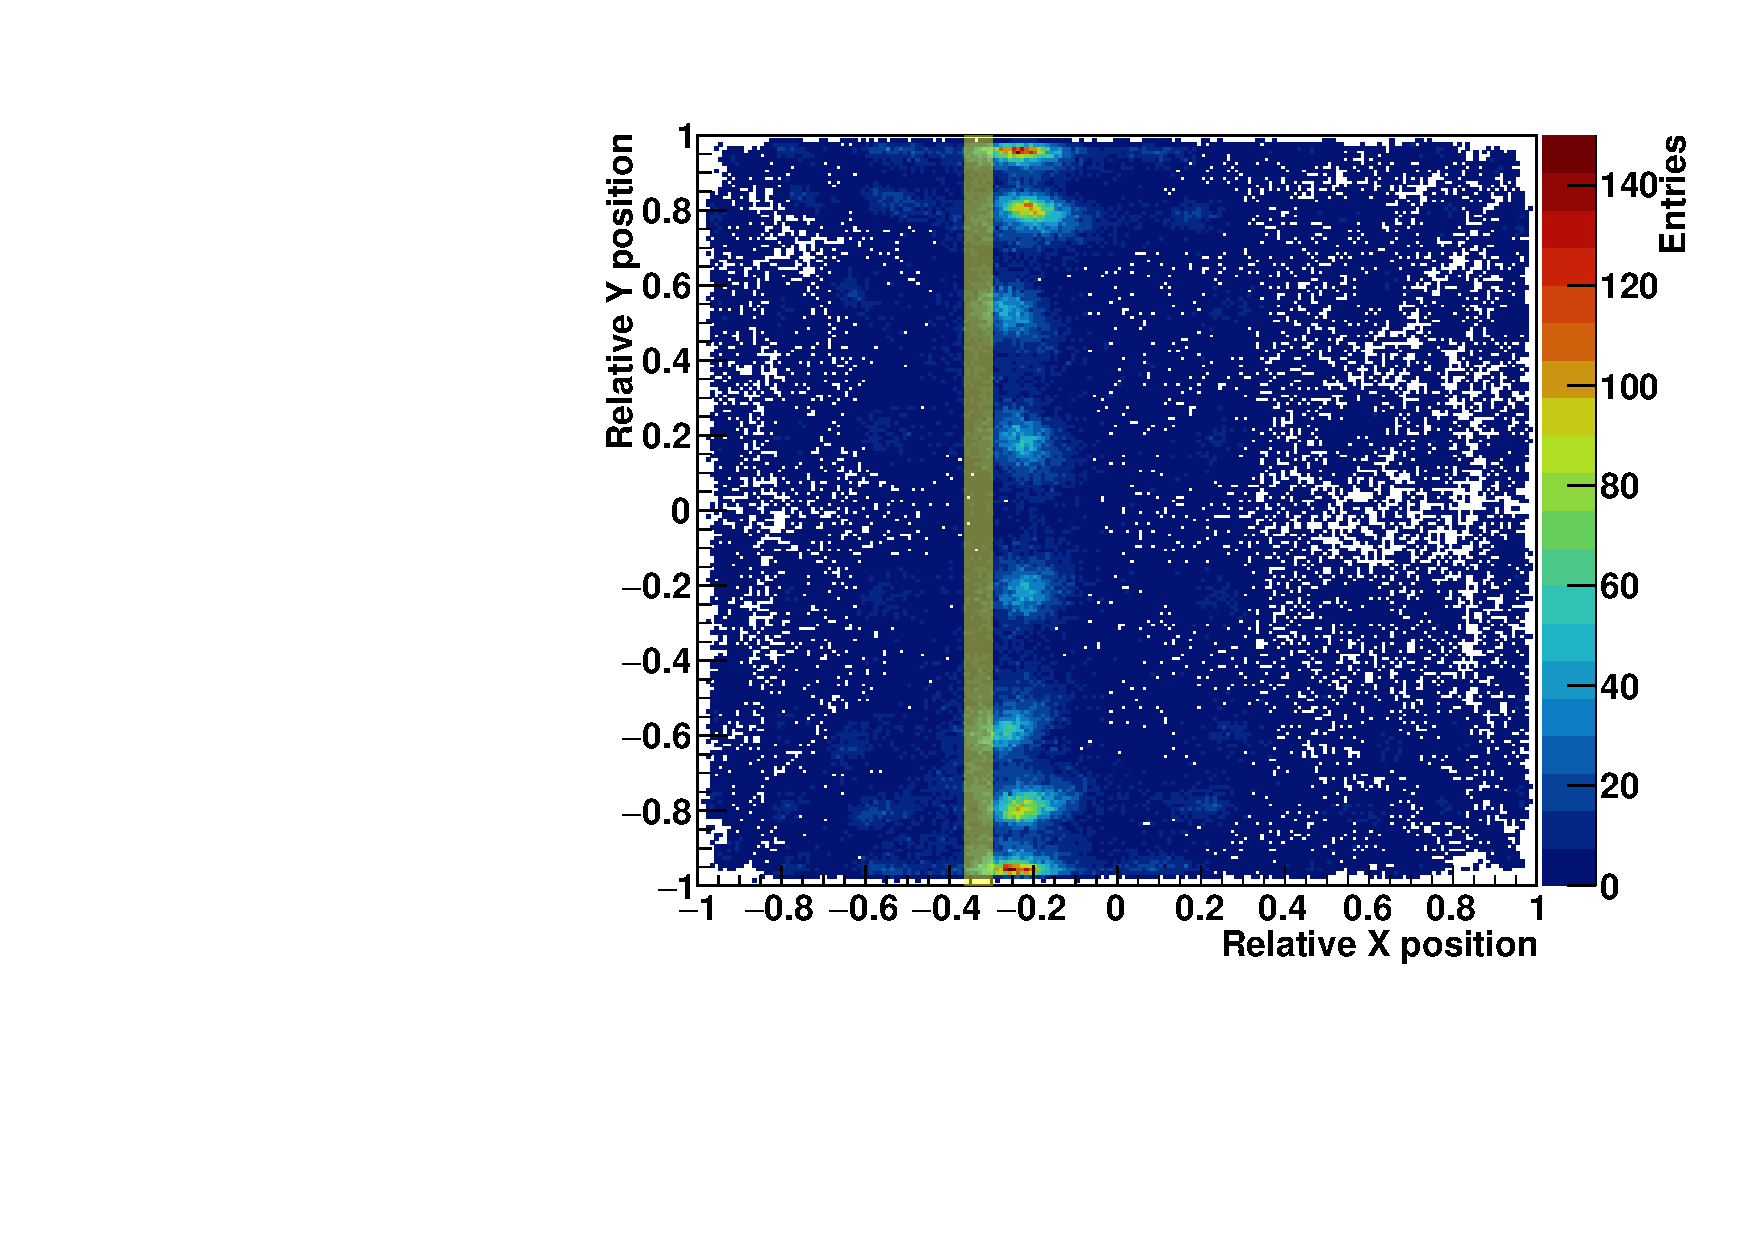
\includegraphics[width=\textwidth]{03_GraphicFiles/chapter3_CLaRySproto/Absorber/images_scan/line_2mm/run11_floodMap.pdf}
\caption{Aperture center relative X position: \\ -0.330}
\label{chap3::fig::scan_map4}
\end{subfigure}
\caption{2D reconstructed position maps during a 2-mm step scan performed with the $^{60}$Co source with the line aperture from the left to the right size of the block surface. 4 reference measurements points, the position of the aperture is shown by the semi-transparent yellow band.}
\label{chap3::fig::ScanFloodMap}
\end{figure}

\begin{figure}
\begin{subfigure}[t]{0.5\textwidth}
\centering
\includegraphics[width=\textwidth]{03_GraphicFiles/chapter3_CLaRySproto/Absorber/images_scan/line_2mm_vert/run12_floodMap.pdf}
\caption{Aperture center relative Y position: \\ -0.100}
\label{chap3::fig::scan_map1_vert}
\end{subfigure}
\begin{subfigure}[t]{0.5\textwidth}
\centering
\includegraphics[width=\textwidth]{03_GraphicFiles/chapter3_CLaRySproto/Absorber/images_scan/line_2mm_vert/run13_floodMap.pdf}
\caption{Aperture center relative Y position: \\ 0.015}
\label{chap3::fig::scan_map2_vert}
\end{subfigure}\newline
\begin{subfigure}[t]{0.5\textwidth}
\centering
\includegraphics[width=\textwidth]{03_GraphicFiles/chapter3_CLaRySproto/Absorber/images_scan/line_2mm_vert/run14_floodMap.pdf}
\caption{Aperture center relative Y position: \\ 0.130}
\label{chap3::fig::scan_map3_vert}
\end{subfigure}
\begin{subfigure}[t]{0.5\textwidth}
\centering
\includegraphics[width=\textwidth]{03_GraphicFiles/chapter3_CLaRySproto/Absorber/images_scan/line_2mm_vert/run15_floodMap.pdf}
\caption{Aperture center relative Y position: \\ 0.245}
\label{chap3::fig::scan_map4_vert}
\end{subfigure}
\caption{2D reconstructed position maps during a 2-mm step scan performed with the $^{60}$Co source with the line aperture from the bottom to the top side of the block surface. 4 reference measurements points, the position of the aperture is shown by the semi-transparent yellow band.}
\label{chap3::fig::ScanFloodMap_Vert}
\end{figure}


\figurename~\ref{chap3::fig::ScanFloodMap} shows four consecutive steps of the $^{60}$Co source collimated irradiation, with a 2-mm step movement from left to right and the linear aperture set in vertical position. A qualitative analysis is enough to appreciate the block spatial accuracy limitation. The presented four points of the scan irradiated a total of three pseudo-pixel columns, moving from the left geometrical border of one column to the center of the next one. As shown by \figurename~\ref{chap3::fig::scan_map2} and~\ref{chap3::fig::scan_map4}, as the collimator aperture position is in front of the center of a pixel column, the whole pseudo-pixel surface is reconstructed, and a better accuracy (2~mm expected, which is the size of the aperture) is not verified. This can be verified by comparing the shown pseudo-pixel columns to the same column in \figurename~\ref{chap3::fig::abscal_floodMap}, obtained with the homogeneous irradiation. In case the aperture faces the border between two pixel columns (\figurename~\ref{chap3::fig::scan_map1} and~\ref{chap3::fig::scan_map3}), the events are shared between the two. This could show a possibility of sub-pixel resolution for integrated measurements, which is anyway not reproducible on a single event basis. The same behavior has been verified with a vertical scan (shown from \figurename~\ref{chap3::fig::scan_map1_vert} to \figurename~\ref{chap3::fig::scan_map4_vert}); the collimator and table configurations has been keep unchanged, while the block has been turned of 90\textdegree.\\ 
In order to further confirm these results, a scan with reduced step size (1~mm) has been performed with the same collimator aperture, and no modifications have been detected in the spatial distribution of events for the steps centered on the same pseudo-pixel column. As before, when the collimator aperture faces the limit between two pseudo-pixels columns, the events are equally distributed on the two. 9 measurement positions for this 1~mm scan are shown from \figurename~\ref{chap3::fig::scan_map1_1mm} to \figurename~\ref{chap3::fig::scan_map9_1mm}.\\ 

\begin{figure}
\centering
\begin{subfigure}[t]{0.32\textwidth}
\centering
\includegraphics[width=\textwidth]{03_GraphicFiles/chapter3_CLaRySproto/Absorber/images_scan/line_1mm/run00014_floodMap.pdf}
\caption{Aperture center relative X position: \\ -0.400}
\label{chap3::fig::scan_map1_1mm}
\end{subfigure}
\begin{subfigure}[t]{0.32\textwidth}
\centering
\includegraphics[width=\textwidth]{03_GraphicFiles/chapter3_CLaRySproto/Absorber/images_scan/line_1mm/run00015_floodMap.pdf}
\caption{Aperture center relative X position: \\ -0.342}
\label{chap3::fig::scan_map2_1mm}
\end{subfigure}
\begin{subfigure}[t]{0.32\textwidth}
\centering
\includegraphics[width=\textwidth]{03_GraphicFiles/chapter3_CLaRySproto/Absorber/images_scan/line_1mm/run00016_floodMap.pdf}
\caption{Aperture center relative X position: \\ -0.285}
\label{chap3::fig::scan_map3_1mm}
\end{subfigure}
\newline
\begin{subfigure}[t]{0.32\textwidth}
\centering
\includegraphics[width=\textwidth]{03_GraphicFiles/chapter3_CLaRySproto/Absorber/images_scan/line_1mm/run00017_floodMap.pdf}
\caption{Aperture center relative X position: \\ -0.227}
\label{chap3::fig::scan_map4_1mm}
\end{subfigure}
\begin{subfigure}[t]{0.32\textwidth}
\centering
\includegraphics[width=\textwidth]{03_GraphicFiles/chapter3_CLaRySproto/Absorber/images_scan/line_1mm/run00018_floodMap.pdf}
\caption{Aperture center relative X position: \\ -0.170}
\label{chap3::fig::scan_map5_1mm}
\end{subfigure}
\begin{subfigure}[t]{0.32\textwidth}
\centering
\includegraphics[width=\textwidth]{03_GraphicFiles/chapter3_CLaRySproto/Absorber/images_scan/line_1mm/run00019_floodMap.pdf}
\caption{Aperture center relative X position: \\ -0.112}
\label{chap3::fig::scan_map6_1mm}
\end{subfigure}
\newline
\begin{subfigure}[t]{0.32\textwidth}
\centering
\includegraphics[width=\textwidth]{03_GraphicFiles/chapter3_CLaRySproto/Absorber/images_scan/line_1mm/run00020_floodMap.pdf}
\caption{Aperture center relative X position: \\ -0.055}
\label{chap3::fig::scan_map7_1mm}
\end{subfigure}
\begin{subfigure}[t]{0.32\textwidth}
\centering
\includegraphics[width=\textwidth]{03_GraphicFiles/chapter3_CLaRySproto/Absorber/images_scan/line_1mm/run00021_floodMap.pdf}
\caption{Aperture center relative X position: \\ 0.003}
\label{chap3::fig::scan_map8_1mm}
\end{subfigure}
\begin{subfigure}[t]{0.32\textwidth}
\centering
\includegraphics[width=\textwidth]{03_GraphicFiles/chapter3_CLaRySproto/Absorber/images_scan/line_1mm/run00022_floodMap.pdf}
\caption{Aperture center relative X position: \\ 0.061}
\label{chap3::fig::scan_map9_1mm}
\end{subfigure}
\caption{2D reconstructed position maps during a 1-mm step scan performed with the $^{60}$Co source with the line aperture. 9 reference measurements points, the position of the aperture is shown by the semi-transparent yellow band.}
\label{chap3::fig::ScanFloodMap_1mm}
\end{figure}

All these set of data verify that the spatial reconstruction accuracy of the employed blocks is limited to the pseudo-pixel size, and a sub-pixel resolution is not achievable on a single event basis. 


\subsubsection{Pixel identification}\label{chap3::subsubsec::absPixelID}

The results of the pixel identification algorithm described in section~\ref{chap3::subsubsec::absPixel_ID_algo} are shown in \figurename~\ref{chap3::fig::abspixID_analysis}. \figurename~\ref{chap3::fig::abslineColID} shows the identified average values of the pseudo-pixels positions on the two transverse dimensions. As already detailed in the description section, starting from these average positions, the single pseudo-pixels positions in rows and columns are extracted and the \enquote{valleys} between neighboring pseudo-pixels are used to define the grid shown in \figurename~\ref{chap3::fig::absfloodWithPix} together with the pseudo-pixel center position map.\\
\begin{figure}
\begin{subfigure}[t]{0.5\textwidth}
\centering
\includegraphics[width=1\textwidth]{03_GraphicFiles/chapter3_CLaRySproto/Absorber/images_charResults_Co60/3_Cal_XYProfiles_withPeaks.pdf}
\caption{1D spatial integrated distributions with reconstructed peaks.}
\label{chap3::fig::abslineColID}
\end{subfigure}
\begin{subfigure}[t]{0.5\textwidth}
\centering
\includegraphics[width=1\textwidth]{03_GraphicFiles/chapter3_CLaRySproto/Absorber/images_charResults_Co60/3_Cal_FLOODMAP_pixels_Regions.pdf}
\caption{2D position map with reconstructed pseudo-pixel centers and areas.}
\label{chap3::fig::absfloodWithPix}
\end{subfigure}
\caption{1D integrated position distributions on the two transverse dimensions with the retrieved position of the pseudo-pixel average center (a). Reconstructed 2D map with the identified pseudo-pixels positions and surfaces.}
\label{chap3::fig::abspixID_analysis}
\end{figure}

\subsubsection{Pixel energy calibration}\label{chap3::subsubsec::absPixelEcal}

Once the pseudo-pixel positions and the related grid are defined, each interaction can be assigned to a single pixel. The energy spectrum of each pixel is then separately studied in order to equalize the energy response on a pixel basis.\\
The assignation method exploits the auxiliary position map shown in \figurename~\ref{chap3::fig::absavPosMap}. The points composing the new map are calculated as the \enquote{valleys} between two neighboring pixels in the two directions (horizontal direction for the red points and vertical direction for the white ones). The column and row points at the minimal distance with respect to the reconstructed interaction position are then identified (and so also the interaction relative position with respect to these two points) and used to calculate the two external products explained in section~\ref{chap3::subsubsec::absPixel_ID_algo}; the sign of the two products uniquely define the pseudo-pixel where to assign the collected event. In \figurename~\ref{chap3::fig::absvectors} an example of the vectors employed for the calculations is presented together with the calculations logic. In \figurename~\ref{chap3::fig::abspixAssCheck} a scheme of the interaction position assignment to the pseudo-pixel is shown: a color has been given to each reconstructed point according to the pseudo-pixel region where it has been assigned by the described method. The method robustness is verified by the comparison of this map to the grid in \figurename~\ref{chap3::fig::absfloodWithPix} and~\ref{chap3::fig::absavPosMap}.   

\begin{figure} [!h]
\centering
\includegraphics[width=0.7\textwidth]{03_GraphicFiles/chapter3_CLaRySproto/Absorber/images_charResults_Co60/3_Cal_FLOODMAP_averPoints.pdf}\\
\caption{Auxiliary position map used for the assignment of the reconstructed events to a single pixel. The highlighted points represent the \enquote{valleys} between neighboring pixels on their separation borders.}
\label{chap3::fig::absavPosMap}
\end{figure}

\begin{figure}
\begin{subfigure}[t]{0.5\textwidth}
\centering
\includegraphics[width=1\textwidth]{03_GraphicFiles/chapter3_CLaRySproto/Absorber/images_charResults_Co60/vector_def.pdf}
\caption{Event assignment to pseudo-pixel logic.}
\label{chap3::fig::absvectors}
\end{subfigure}
\begin{subfigure}[t]{0.5\textwidth}
\centering
\includegraphics[width=1\textwidth, height = 6cm]{03_GraphicFiles/chapter3_CLaRySproto/Absorber/images_charResults_Na22/3_2PixelAssignment.png}
\caption{2D map of the reconstructed event assignations to pseudo-pixels.}
\label{chap3::fig::abspixAssCheck}
\end{subfigure}
\caption{Logic for the event assignment to a single pixel (left) and 2D map of the resulting interaction assignment (right): each event is colored according to the chosen pseudo-pixel. }
\label{chap3::fig::abspixAssignment}
\end{figure}

In \figurename~\ref{chap3::fig::abspixCal_analysis} the results of the pseudo-pixel energy calibration are shown. \figurename~\ref{chap3::fig::abssinglePixCal} (left) shows the overlap of the energy spectra for 60 pseudo-pixels before the energy calibration and equalization. The 4 pseudo-pixels on the corners show a very different energy response and are not included in this picture. This is probably due to a not complete light collection. The different response of each pixel to the two energy peaks is clearly visible. For each spectrum the low energy peak is assigned to 511~keV, while the high energy one to 1275~keV. In this way, the spectra are linearly calibrated and equalized, as shown in \figurename~\ref{chap3::fig::abssinglePixCal} (right). For the 4 corner pseudo-pixels, the calibration is based only on the 1275~keV peak, while the 511~keV reference peak is substituted by the null ADC value.\\
Once the single pixel energy responses are equalized and calibrated, the whole block energy spectrum can be derived with the sum of the all pixels. In \figurename~\ref{chap3::fig::absEspectrumCal} (left) the \gls{adc} spectrum is shown before the equalization process, while in \figurename~\ref{chap3::fig::absEspectrumCal} (right) the calibrated energy spectrum is presented. In \figurename~\ref{chap3::fig::absEspectrumCal} (left) the energy spectra related to three reference position on the block surface are reported: this makes possible to appreciate  the different contributions to the non-calibrated spectrum and the behavior of different block sections. The block peripheral pixels show an overall lower light collection and probably include a large amount of non completely absorbed events. Concerning the central pixels, the slight in-homogeneity is probably due to the streaked structure which guides less than on the borders the scintillation photons.\\
The two spectra are represented in logarithmic scale in order to better appreciate the calibration effect: it allows to optimize the energy response on the two spectroscopic lines of the $^{22}$Na source. At this stage, the energy resolutions of the block can be defined as the \gls{fwhm} of the two energy peaks.\\
In \tablename~\ref{chap3::tab::absresComp}, the energy resolutions derived after the calibration process are compared to the raw ones, obtained by the non-calibrated data.


\begin{table}[!htbp]
\centering
\caption{Comparison of the results obtained with the two pixel-assignment methods.}
\label{chap3::tab::absresComp}
\begin{tabular}{P{3cm} P{4cm} P{4cm}}
\toprule
\rowcolor{myColorMainA!20} 
 	& \textbf{Energy resolution} & \textbf{Energy resolution} \\
\rowcolor{myColorMainA!20} 
	& \textbf{@ 511~keV} & \textbf{@ 1275~keV } \\
\rowcolor{myColorMainA!20} 
 	& \textbf{\gls{fwhm} [\%]} & \textbf{\gls{fwhm} [\%]} \\
\midrule
\textbf{Before} & 46.12& 39.43\\
\textbf{equalization} & [\% ADC counts]& [\% ADC counts]\\
\midrule

\textbf{After} &23.03& 18.04 \\
\textbf{equalization} & [\% keV]& [\% keV]\\
\bottomrule
\end{tabular}
\end{table}

The results reported in \tablename~\ref{chap3::tab::absresComp} show the need for the implemented calibration process, which allows to optimize the \gls{bgo} block spatial and energy response. 

\begin{figure}
\begin{subfigure}[t]{1\textwidth}
\centering
\includegraphics[width=0.8\textwidth]{03_GraphicFiles/chapter3_CLaRySproto/Absorber/images/EspectraOverlap_noAngles.pdf}
\caption{Single pixel energy spectrum before (left) and after (right) equalization.}
\label{chap3::fig::abssinglePixCal}
\end{subfigure}
\begin{subfigure}[t]{1\textwidth}
\centering
\includegraphics[width=0.8\textwidth]{03_GraphicFiles/chapter3_CLaRySproto/Absorber/images/Espectra_withSingles.pdf}
\caption{Block energy spectrum before (left) and after (right) pixel response equalization.}
\label{chap3::fig::absEspectrumCal}
\end{subfigure}
\caption{Single pseudo-pixels (a) and whole block (b) energy spectra with the $^{22}$Na source before (left) and after (right) the calibration process. The whole block spectra are reported in logarithmic scale. Three non calibrated spectra of pixels in reference positions (border, mid-center and center area) on the block are also reported with the non calibrated spectrum.}
\label{chap3::fig::abspixCal_analysis}
\end{figure}

Thanks to the assignment of each reconstructed event to a single pseudo-pixel, the relative efficiency can be evaluated on a single pseudo-pixel basis. The two color maps in \figurename~\ref{chap3::fig::absefficiency} show the number of events collected by the 64 pseudo-pixels during the $^{22}$Na source homogeneous irradiation, with an energy selection performed on the two photons energy emitted by the source (511~keV events in \figurename~\ref{chap3::fig::abseffLE} and 1275~keV events in \figurename~\ref{chap3::fig::abseffHE}). The entries are normalized to the maximum number of entries in a pseudo-pixel, detected for a 511~keV energy selection.

\begin{figure}
\begin{subfigure}[t]{0.5\textwidth}
\centering
\includegraphics[width=1\textwidth]{03_GraphicFiles/chapter3_CLaRySproto/Absorber/images/eff_map_LE_norm.pdf}
\caption{511~keV.}
\label{chap3::fig::abseffLE}
\end{subfigure}
\begin{subfigure}[t]{0.5\textwidth}
\centering
\includegraphics[width=1\textwidth]{03_GraphicFiles/chapter3_CLaRySproto/Absorber/images/eff_map_HE_norm.pdf}
\caption{1275~keV.}
\label{chap3::fig::abseffHE}
\end{subfigure}
\caption{Relative number of entries for each pseudo-pixel as a function of the pixel relative position, represented by the row and column numbers (0 to 8 from left to right and bottom to top of the block surface). \figurename (a) shows the entries in a selected energy window around 511~keV, \figurename (b) in an energy window around 1275~keV. All the entries are normalized to the maximum collected number of entries, corresponding to 511~keV events in the central section of the block.}
\label{chap3::fig::absefficiency}
\end{figure}

Figures~\ref{chap3::fig::abseffLE} and~\ref{chap3::fig::abseffHE} show that the expected homogeneous distribution of events over the whole block surface is confirmed for the central pseudo-pixels of central lines (1 to 6), while the block borders present a factor 2-3 lower detection efficiency. In particular, the pseudo-pixels on the 4 corners (line 0 and 7, pseudo-pixels 0 and 7), have an efficiency of a factor between 5 and 6 lower with respect to the center of the block surface. This effect is partially due to geometrical factors, given the fact that the side pseudo-pixels are slightly smaller with respect to the central one (as also shown by the reconstructed 2D map in \figurename~\ref{chap3::fig::absfloodWithPix}). In addition to this, the light collection is probably less performing in case of photons interacting on the block borders, causing the lost of events. By comparing the two maps, an overall reduced efficiency for the detection of photons beyond 1~MeV is verified. This is expected given the photons full absorption probability in \gls{bgo} at 511~keV and 1275~keV, estimated in about 80\% and 70\% respectively. In order to fully understand the relative and absolute efficiency of each block section, an irradiation with a collimated source scanning the whole active area is foreseen. This will allow one to precisely define the detection rate variations on the block active area.

\subsubsection{Time characterization}\label{chap3::subsubsec::timeChar}

\figurename~\ref{chap3::fig::abstimeDiff} shows the distribution of arrival time differences between the reference \gls{baf2} detector and the tested \gls{bgo} block. The time resolution is defined as the \gls{fwhm} of this distribution.

\begin{figure}
 \centering
  \includegraphics[width=0.7\textwidth]{03_GraphicFiles/chapter3_CLaRySproto/Absorber/images/timeDiff_distr.pdf}
  \caption{Distribution of arrival time differences between reference scintillator and \gls{bgo} block.}	
  \label{chap3::fig::abstimeDiff}
\end{figure}

\subsubsection{Results for the 30 blocks}\label{chap3::subsubsec::30blocksRes}

In \tablename~\ref{chap3::tab::absresults30Blocks} the results obtained for the calibration and characterization of a set of 10 blocks are listed.
The characterized blocks show very uniform results, with an average energy resolution of 25\% \gls{fwhm} at 511~keV and 20\% \gls{fwhm} at 1275~keV and an average time resolution of 4.42~ns \gls{fwhm} tested with coincidences of 511~keV photons. Both the energy and time resolution are expected to be improved for the detection of photons in the prompt-gamma energy range, in particular above 1~MeV.

\begin{table}[!htbp]
\centering
\caption{Calibration  and characterization results for 10 tested \gls{bgo} blocks.}
\label{chap3::tab::absresults30Blocks}
\begin{tabular}{P{2.8cm} P{3.6cm} P{3.6cm} P{3.6cm}}
\toprule
\rowcolor{myColorMainA!20} 
\textbf{\gls{bgo} block} 	& \textbf{Energy resolution} & \textbf{Energy resolution} & \textbf{Time}\\
\rowcolor{myColorMainA!20} 
\textbf{ID} 	& \textbf{@ 511~keV} & \textbf{@ 1275~keV } & \textbf{resolution}\\
\rowcolor{myColorMainA!20} 
 	& \textbf{\gls{fwhm} [\%]} & \textbf{\gls{fwhm} [\%]} & \textbf{\gls{fwhm} [ns]}\\
\midrule
\textbf{Ref. block} & & &\\
\textbf{7627} & \textbf{23}& \textbf{18}& \textbf{4.0}\\
\midrule
3166 & 27& 24& 4.4\\
3171 & 23& 18& 4.4\\
3184 & 24& 20& 4.3\\
3232 & 24& 20& 3.6\\
3280 & 24& 19& 4.3\\
3322 & 25& 20& 4.2\\
3972 & & & 5.2\\
4368 & 25& 20& 5.3\\
5243 & 25 & 19 & 3.9\\
6823 & & & 1.7\\
7130 & & & 4.9\\
7218 & 25& 21& 2.1\\
7240 & 25& 20& 6.7\\
7258 & 26& 19& 4.9\\
7369 & 23& 19& 4.3\\
7424 & 25& 21& 4.9\\
7581 & 26& 23& 4.1\\
7586 & 26& 24& 4.4\\
7601 & 24& 19& 4.1\\
7612 & 23& 19& 4.1\\
7624 &   &   & 3.9\\
7651 & 24& 20& 3.9\\
7657 & 24& 19& 2.7\\
14676 & 25& 19& 5.1\\
31210 & 25& 21& 4.8\\
\midrule
3252 & \multicolumn{3}{c}{problem with \gls{pm} 0}\\
3375 & \multicolumn{2}{c}{1 pseudo-pixel missing} & 6.4\\
7644 & \multicolumn{3}{c}{problem with \gls{pm} 2}\\
7653 & \multicolumn{2}{c}{1 pseudo-pixel missing} & 2.3\\
21097 & \multicolumn{3}{c}{problem with \gls{pm} 2}\\

\midrule
\textbf{Complete set} & 25 $\varpm$ 1& 20 $\varpm$ 2& 4.4 $\varpm$ 0.5\\
\bottomrule
\end{tabular}
\end{table}

The last five blocks in the list of \tablename~\ref{chap3::tab::absresults30Blocks} showed detection problems, due to very low signal level on the read-out \glspl{pm} or a poor spatial reconstruction accuracy with one missing pseudo-pixel on the two-dimensional map, probably due to crystal aging. The blocks with \glspl{pm} issues will not be employed in the final absorber configuration, while the other two will be probably placed in the peripheral area in order to keep a wide active detection surface.   

\newpage

\subsection{Hodoscope \glspl{pm} characterization}\label{chap3::subsec::hodoPMchar}         

The beam tagging hodoscope read-out is performed via 8 multi-anode \glspl{pm}, Hamamatsu H8500~\parencite{Hamamatsu2006}, shown in \figurename~\ref{chap3::fig::PMH8500}. In order to guarantee a uniform response of the whole detector active area, composed of 256 scintillating fibers, the \glspl{pm} must be previously characterized in terms of gain with a light source of fixed and known wave-length and intensity. The source selected for the measurements is a blue \gls{led} (Hewlett-Packard HLMP-CB), installed on the test-bench shown in \figurename~\ref{chap3::fig::hodo_testBenchPM} and described in the following. The test-bench has been developed by the \gls{lpc} \gls{avirm} group (see~\cite{Gaglione2013}) and adapted at the \gls{ipnl} to a different acquisition system.\\
The goal of the characterization measurements is to trace a gain map of the whole \gls{pm} surface, with the aim of storing calibration data to be used to both tune the \gls{pm} working parameters (supply voltage and threshold) and correct the collected data. This is achieved by scanning the \gls{pm} photo-cathode surface with the \gls{led}. The \gls{led} is so mounted on a motorized double-axis table, controlled by two G203V stepper modules provided by GeckoDrive Motor Controls~\parencite{GeckoDrive2010}. The two axes have a total range of 20~cm each, and the step resolution achieved by the controllers is 20~\charmum. A metal support is set on the table in order to fix the \gls{led}. It produces light pulses synchronized with a pulse generator, which is also used as trigger signal for the acquisition system, as detailed later. The light pulse produced by the \gls{led} is split into two pulses with a 45\textdegree{} mirror: one pulse is sent to the H8500 \gls{pm} to be tested via optical fiber, in order to obtain a light beam perpendicular to the cathode surface (\gls{fwhm} beam width estimated in 0.5~mm), the second one is detected by an Hamamatsu R5600 \gls{pm}~\parencite{Hamamatsu1995}, used as reference for the correction of temperature fluctuations. The \gls{pm} under tests is fixed below the optical fiber output with a plastic support, not connected to the moving table. The whole described system is contained in a black box for external light shielding.\\
The output signals from the H8500 \gls{pm} are initially amplified by custom pre-amplification cards: 8 cards are available and have been characterized in terms of amplification gain. Once amplified, the signals of the H8500 \gls{pm}, together with the output of the reference \gls{pm}, are sent to the acquisition system composed of a National Instrument PXI Express 1082~\parencite{NationalInstruments2010} equipped with two 8-channel flash \gls{adc} modules (NI PXI-5105) and a two-channel ultra-fast digitizer (NI PXI-5154). The flash \gls{adc} modules have a maximum sampling rate of 60~MHz and are used for the read-out of the H8500 \gls{pm} signals, while the ultra-fast digitizer, able to sample at a frequency up to 1~GHz, is used for the reference \gls{pm}.\\
The acquisition and control software is developed with LabVIEW (2009) installed on the PXI; a picture of the software user interface is shown in \figurename~\ref{chap3::fig::hodo_LabView}. The PXI receives the signals from the two \glspl{pm} and is also connected to the table stepper modules, so that the LabVIEW software can handle and synchronize data acquisition and table movements. The table movements can be automatized via LabVIEW macros, where step size, number and direction are stored and then used for the acquisition. The acquisition trigger, as mentioned, is given by the pulse generator which also control the light pulses of the \gls{led}; in this way, a fixed number of pulses per table position can be recorded, and the measurement process is completely automatic. During the acquisition, the LabVIEW software automatically corrects the collected data according to the reference \gls{pm} signal amplitude and to the pre-amplification card gain.\\
Given the limited number of flash \gls{adc} channels, only 16 \gls{pm} pixels can be characterized per acquisition; four acquisitions are needed to scan the complete \gls{pm} surface.\\
 
\begin{figure}
\begin{subfigure}[t]{1\textwidth}
\centering
\includegraphics[width=0.7\textwidth]{03_GraphicFiles/chapter3_CLaRySproto/Hodoscope/testBenchPM.jpg}
\caption{Overview of the test-bench setup for the Hamamatsu \glsps{pm} characterization.}
\label{chap3::fig::hodo_testBenchPM}
\end{subfigure}
\newline
\begin{subfigure}[t]{.5\textwidth}
\centering
\includegraphics[width=1\textwidth, height = 5.cm]{03_GraphicFiles/chapter3_CLaRySproto/Electronics_Acquisition/PXI_ipnl.jpg}
\caption{National Instruments PXIe acquisition system.}
\label{chap3::fig::PXI_NI}
\end{subfigure}
\begin{subfigure}[t]{.5\textwidth}
\centering
\includegraphics[width=1\textwidth, height = 5.cm]{03_GraphicFiles/chapter3_CLaRySproto/Hodoscope/hodoTests.jpg}
\caption{Example of LabVIEW software interface for the Hamamatsu 	\glspl{pm} characterization.}
\label{chap3::fig::hodo_LabView}
\end{subfigure}
\caption{Test-bench and tools for the characterization measurements performed on the Hamamatsu \glspl{pm} of the beam tagging hodoscope.}
\label{chap3::fig::hodoPMtest}
\end{figure}

Each performed acquisition is set to scan a matrix of 4$\times$4 \gls{pm} pixels, and safety margins are arranged on the \gls{pm} sides in order to ensure a complete surface irradiation. As shown in the schematic view of the \gls{pm} in \figurename~\ref{chap3::fig::hodoPMscheme}, the total \gls{pm} size is 52$\times$52~mm$^{2}$, for an active area of about 49$\times$49~mm$^{2}$. The active area of the pixels on the borders is slightly wider than the central ones. In order to optimize the measurement process, a preliminary analysis has been done for the definition of the needed step length, and the details are reported in~\cite{Coudurier2015}. A trade-off between measurement accuracy, required time and stored data file size has been found with a step of 800~\charmum, so that each pixel is scanned with approximately 64 measurement points and the transition between neighboring pixels can be appreciated. A schematic of a table reference movement is presented in \figurename~\ref{chap3::fig::hodoPMscanScheme}. To be noticed that for each irradiated point, 100 \gls{led} pulses are sent to the detector and the average amplitude value is calculated and collected.\\  
The 8 Hamamatsu \glspl{pm} have been completely scanned without the optical fiber mask used in the hodoscope and shown in \figurename~\ref{chap3::fig::PMmask}, and the results are shown here for one reference \gls{pm}. Some tests have been also performed with the fiber mask, in order to test the \gls{pm} response mainly in terms of expected cross-talk between neighboring pixels. A complete result database has been created for calibration purpose.\\

\begin{figure}
\begin{subfigure}[t]{.5\textwidth}
\centering
\includegraphics[width=1\textwidth]{03_GraphicFiles/chapter3_CLaRySproto/Hodoscope/PM_specs_mod.pdf}
\caption{Scheme and quotation of the Hamamatsu H8500 multi-anode \glspl{pm}.}
\label{chap3::fig::hodoPMscheme}
\end{subfigure}
\begin{subfigure}[t]{.5\textwidth}
\centering
\includegraphics[width=1\textwidth]{03_GraphicFiles/chapter3_CLaRySproto/Hodoscope/scan_logic.pdf}
\caption{Scheme of the scan performed for the Hamamatsu \gls{pm} characterization measurements.}
\label{chap3::fig::hodoPMscanScheme}
\end{subfigure}
\caption{Details of the hodoscope \glspl{pm} and of the performed characterization measurements.}
\label{chap3::fig::hodoScanDetails}
\end{figure}

\figurename~\ref{chap3::fig::hodoPMchar2DnoMask} shows the two-dimensional maps of a reference \gls{pm} response for a complete irradiation, obtained with four separated acquisitions without the plastic fiber mask. \figurename~\ref{chap3::fig::hodoPMchar2DwithMask} shows the response of the same \gls{pm} with the plastic fiber mask fixed on its surface. The reported signal amplitude has been normalized to the reference \gls{pm} Hamamatsu R5600 for temperature oscillation correction, but the relative difference between the two irradiation is maintained to show the signal attenuation caused by the fiber mask, resulting in a factor 3-4 depending on the pixel.\\ 

\begin{figure}
\begin{subfigure}[t]{.5\textwidth}
\centering
\includegraphics[width=1\textwidth, height = 5.8cm ]{03_GraphicFiles/chapter3_CLaRySproto/Hodoscope/PMchar/Maps_noMask/2DMap_PM2_notNorm.png}
\caption{2D map without fiber mask.}
\label{chap3::fig::hodoPMchar2DnoMask}
\end{subfigure}
\begin{subfigure}[t]{.5\textwidth}
\centering
\includegraphics[width=1\textwidth, height = 5.8cm ]{03_GraphicFiles/chapter3_CLaRySproto/Hodoscope/PMchar/Maps_withMask/2DMap_PM2_notNorm.png}
\caption{2D map with fiber mask.}
\label{chap3::fig::hodoPMchar2DwithMask}
\end{subfigure}
\caption{Two-dimensional response maps of one of the Hamamatsu \glspl{pm} for the scintillating fiber hodoscope readout, obtained with the irradiation with a blue 	\gls{led}. The signal amplitude is normalized to the reference \gls{pm} response.}
\label{chap3::fig::hodoPMchar2Dmaps}
\end{figure}


\begin{figure}
\begin{subfigure}[t]{.5\textwidth}
\centering
\includegraphics[width=0.8\textwidth]{03_GraphicFiles/chapter3_CLaRySproto/Hodoscope/PMchar/Maps_noMask/2DMap_PM1_Norm.png}
\caption{\gls{pm} 1 2D map without fiber mask.}
\label{chap3::fig::hodoPMchar2DnoMask_pm1}
\end{subfigure}
\begin{subfigure}[t]{.5\textwidth}
\centering
\includegraphics[width=0.8\textwidth]{03_GraphicFiles/chapter3_CLaRySproto/Hodoscope/PMchar/Maps_noMask/2DMap_PM2_Norm.png}
\caption{\gls{pm} 2 2D map without fiber mask.}
\label{chap3::fig::hodoPMchar2DnoMask_pm2}
\end{subfigure}
\begin{subfigure}[t]{.5\textwidth}
\centering
\includegraphics[width=0.8\textwidth]{03_GraphicFiles/chapter3_CLaRySproto/Hodoscope/PMchar/Maps_noMask/2DMap_PM3_Norm.png}
\caption{\gls{pm} 3 2D map without fiber mask.}
\label{chap3::fig::hodoPMchar2DnoMask_pm3}
\end{subfigure}
\begin{subfigure}[t]{.5\textwidth}
\centering
\includegraphics[width=0.8\textwidth]{03_GraphicFiles/chapter3_CLaRySproto/Hodoscope/PMchar/Maps_noMask/2DMap_PM4_Norm.png}
\caption{\gls{pm} 4 2D map without fiber mask.}
\label{chap3::fig::hodoPMchar2DnoMask_pm4}
\end{subfigure}
\begin{subfigure}[t]{.5\textwidth}
\centering
\includegraphics[width=0.8\textwidth]{03_GraphicFiles/chapter3_CLaRySproto/Hodoscope/PMchar/Maps_noMask/2DMap_PM5_Norm.png}
\caption{\gls{pm} 5 2D map without fiber mask.}
\label{chap3::fig::hodoPMchar2DnoMask_pm5}
\end{subfigure}
\begin{subfigure}[t]{.5\textwidth}
\centering
\includegraphics[width=0.8\textwidth]{03_GraphicFiles/chapter3_CLaRySproto/Hodoscope/PMchar/Maps_noMask/2DMap_PM6_Norm.png}
\caption{\gls{pm} 6 2D map without fiber mask.}
\label{chap3::fig::hodoPMchar2DnoMask_pm6}
\end{subfigure}
\begin{subfigure}[t]{.5\textwidth}
\centering
\includegraphics[width=0.8\textwidth]{03_GraphicFiles/chapter3_CLaRySproto/Hodoscope/PMchar/Maps_noMask/2DMap_PM7_Norm.png}
\caption{\gls{pm} 7 2D map without fiber mask.}
\label{chap3::fig::hodoPMchar2DnoMask_pm7}
\end{subfigure}
\begin{subfigure}[t]{.5\textwidth}
\centering
\includegraphics[width=0.8\textwidth]{03_GraphicFiles/chapter3_CLaRySproto/Hodoscope/PMchar/Maps_noMask/2DMap_PM8_Norm.png}
\caption{\gls{pm} 8 2D map without fiber mask.}
\label{chap3::fig::hodoPMchar2DnoMask_pm8}
\end{subfigure}
\caption{Two-dimensional response maps of the Hamamatsu \glspl{pm} for the scintillating fiber hodoscope readout, obtained with the irradiation with a blue 	\gls{led}. The signal amplitude is normalized to the reference \gls{pm} response and then to each \gls{pm} maximum detected amplitude.}
\label{chap3::fig::hodoPMchar2Dmaps_allPM}
\end{figure}

In \figurename~\ref{chap3::fig::hodoPMchar2Dmaps_allPM} the two-dimensional response map for the 8 \glspl{pm} are shown. In order to obtain a visual uniformity, the amplitude values have been normalized to the maximum value of each \gls{pm}. We can observe response dis-uniformity on each \gls{pm} surface, estimated in a factor ranging between 2 and 3. The retrieved response of each pixel will be useful for the calibration of the hodoscope final acquisition chain, in particular for what concerns the electronics \gls{fe} settings (threshold and gain of each channel). In addition to this, these calibration measurements will allow for a proper data correction at the analysis stage.\\
The irradiation performed with the fiber plastic mask are also used to study the signal cross-talk between neighboring pixels, which is expected to be negligible according to the provider specifications, given for similar measurements and shown in \figurename~\ref{chap3::fig::hodoPMcharcross-talkSpec}. The analysis results for one of the studied \glspl{pm} are shown in \figurename~\ref{chap3::fig::hodoPMcharcross-talkMeas} as reference.
      
\begin{figure}
\begin{subfigure}[t]{.5\textwidth}
\centering
\includegraphics[width=1\textwidth, trim={0 6cm 0 6cm}, clip=true]{03_GraphicFiles/chapter3_CLaRySproto/Hodoscope/PMchar/cross_talk_spec.pdf}
\caption{Signal cross-talk provided by Hamamatsu for the \gls{pm} H8500~\parencite{Hamamatsu2006}. The measurements have been performed with a 1~mm diameter optical fiber; the irradiated anode is in the light blue box, and the cross-talk on the neighboring ones is expressed in \%.}
\label{chap3::fig::hodoPMcharcross-talkSpec}
\end{subfigure}
\begin{subfigure}[t]{.5\textwidth}
\centering
\includegraphics[width=1\textwidth]{03_GraphicFiles/chapter3_CLaRySproto/Hodoscope/PMchar/cross_talk_join_PM2_withMask.png}
\caption{Signal cross-talk on a reference \gls{pm} measured with a blue \gls{led} irradiation through the plastic fiber mask. The irradiated anode is in the light blue box, and the cross-talk on the neighboring ones is expressed in \%.}
\label{chap3::fig::hodoPMcharcross-talkMeas}
\end{subfigure}
\caption{Cross-talk study on neighboring \gls{pm} pixels. The experimental results obtained with the irradiation with a blue \gls{led} through the plastic fiber mask on a reference \gls{pm} (right) are compared to the specifications provided by the producer, measured in similar conditions (left). The cross-talk is expressed in \% with respect to the irradiated anode, which is represented by the light-blue cell with 100\% of the signal.}
\label{chap3::fig::hodoPMcharCross-Talk}
\end{figure}

The retrieved cross-talk is more important with respect to the provider specifications (to be noticed that the measurement conditions are slightly different), but always below 3\% for the tested anodes. This cross-talk level is negligible and can be easily suppressed by a proper threshold setting.\\

\subsection{Hodoscope fiber test with electron source}\label{chap3::subsec::hodoBetatest}

After the complete characterization of the Hamamatsu multi-anode \glspl{pm}, they have been installed in the black boxes connected to the optical fibers of the hodoscope prototype, and the complete detection chain have been qualitatively tested to check the scintillating fiber light transmission to the optical fibers and to the read-out \glspl{pm}. The observations have been performed by directly checking the pre-amplified \gls{pm} output signal (with the same custom cards mentioned in the previous section) on an oscilloscope. A mechanical intervention has been necessary to fix some of the optical fibers not properly pasted to the plastic mask on the \gls{pm} surface. In addition to this, a layer of black silicone has been added on the plastic mask surface to improve the light isolation on the only side where it is impossible to place the isolating black tape.\\
The hodoscope prototype has been then tested with a beta source ($^{90}$Sr) for verification, and the obtained signal distributions (retrieved as before with an oscilloscope acquisition after signal pre-amplification) have been compared to simulation study performed by an internship Master 1 student~\parencite{Vallois2016}. He tested in simulation the irradiation of the whole hodoscope surface with an equivalent $^{90}$Sr source to retrieve the deposited energy distribution on the scintillating fibers. This distribution can be compared to the collected signals amplitude distribution obtained with the experimental tests, in order to calibrate the relationship signal amplitude-deposited energy. The distance between the source and the fiber was set to 3 mm in the simulation code, to reproduce the gap created by the plastic box of the real source, which was directly  on the fiber for the experimental measurements. In \figurename~\ref{chap3::fig::hodoSimuData} the results for a reference fiber are shown. The distribution entries have been normalized to the total number of events for visualization purpose.

\begin{figure}[htb]
\centering
\includegraphics[width=0.8\textwidth]{03_GraphicFiles/chapter3_CLaRySproto/Hodoscope/dEdistrComparison.pdf}
\caption{Comparison of the simulated distribution of energy deposited by electrons from the $^{90}$Sr source on a single hodoscope fiber to the experimental signal amplitude distribution from a scintillating fiber irradiated with the $^{90}$Sr source.}
\label{chap3::fig::hodoSimuData}
\end{figure}

The comparison presented in \figurename~\ref{chap3::fig::hodoSimuData} can be useful as estimate of the expected signal for a given energy deposited by a ionizing particle (about 50~mV for about 200~keV of energy deposited). Knowing the applied amplification factor (given by the per-amplification card characterization) and the relative gain of each \gls{pm} pixel, the expected raw signal integral can be estimated.\\
A complete characterization of the hodoscope acquisition chain will be necessary on proton and carbon beams in order to verify the beam primaries energy deposit on the scintillating fibers and tune the working parameters. In particular, the increased energy deposit expected for proton and carbons with respect to electrons should allow for a reduction of the high voltage applied to the \gls{pm}. With reduced voltage, the detection rate capability would be improved. All these assumption will be tested on beam in the next future.

ADD HERE THE RESULTS OF THE SUMMER ABOUT THE ASIC GAIN AND THRESHOLD CHARACTERIZATION, AND COMMENT LINKING TO CHAPTER 6 FOR THE BEAM TESTS. 

\newpage

%%%%%%%%%%%%%%%%%%%%%%%%%%%%%%%%%%   NEXT  %%%%%%%%%%%%%%%%%%%%%%%%%%%%%%%%%%%%%%%%%%%%

\section{Summary and perspectives}\label{chap3::sec::Next}

The \gls{clarys} collaboration is developing in parallel two gamma cameras for ion beam therapy monitoring and nuclear medicine applications. At present, the detector components are being tested separately for characterization purposes at the \gls{ipnl}. I presented in this chapter a complete description of the detector components with the related \gls{fe} electronics, mechanical support, acquisition system and software tools, together with the all the characterization measurements I performed on the various detector sections. In the following, in addition to a short summary of the present status of the instrumental development of each camera component, I list the main task to be accomplished for the final integration a complete operation of the whole camera. 

\subsection{Silicon scatterer}\label{chap3::subsec::scattNext}
Among the 10 \gls{dssd} layer provided by the seller, only 7 respected the design requirements and have been selected for the use in the Compton camera prototype. The 7 selected layer have been characterized in terms of leakage current with an acquisition system specifically developed for this purpose. Temperature cycles have been performed in order to precisely define the cooling performance needed to obtained the required noise level. These measurements allow to fix the working temperature to -20\textdegree{} and lead to the conception and production of a thermal regulated box, working with cold air and so adapted to the clinical use. A modular mechanical support has been fixed inside the camera to sustain the silicon layers with their \gls{fe} cards. The \gls{fe} card has been designed and tested at the \gls{ipnl}, and includes a custom \gls{asic} which have been optimized with three different developed versions. The final version of the whole board have been produced in 7 copies in 2017 and they are now available for the next test stages.\\
   

\subsection{\gls{bgo} absorber}\label{chap3::subsec::absNext}

\subsection{Scintillating fiber hodoscope}\label{chap3::subsec::hodoNext}

\subsection{Electronics and acquisition}\label{chap3::subsec::daqNext}

%\subsection{}\label{chap3::subsec::}




\clearpage
%\printbibliography[heading=subbibintoc]
